\documentclass[a4paper]{book}
\usepackage{a4wide}
\usepackage{makeidx}
\usepackage{graphicx}
\usepackage{multicol}
\usepackage{float}
\usepackage{listings}
\usepackage{color}
\usepackage{textcomp}
\usepackage{alltt}
\usepackage[utf8]{inputenc}
\usepackage{doxygen}
\lstset{language=C++,inputencoding=utf8,basicstyle=\footnotesize,breaklines=true,breakatwhitespace=true,tabsize=8,numbers=left }
\makeindex
\setcounter{tocdepth}{3}
\renewcommand{\footrulewidth}{0.4pt}
\begin{document}
\begin{titlepage}
\vspace*{7cm}
\begin{center}
{\Large ccAudio }\\
\vspace*{1cm}
{\large Generated by Doxygen 1.6.1}\\
\vspace*{0.5cm}
{\small Mon May 3 04:03:16 2010}\\
\end{center}
\end{titlepage}
\clearemptydoublepage
\pagenumbering{roman}
\tableofcontents
\clearemptydoublepage
\pagenumbering{arabic}
\chapter{Namespace Index}
\section{Namespace List}
Here is a list of all namespaces with brief descriptions:\begin{DoxyCompactList}
\item\contentsline{section}{{\bf ost} }{\pageref{namespaceost}}{}
\end{DoxyCompactList}

\chapter{Class Index}
\section{Class Hierarchy}
This inheritance list is sorted roughly, but not completely, alphabetically:\begin{DoxyCompactList}
\item \contentsline{section}{ost::Bayonne}{\pageref{classost_1_1_bayonne}}{}
\begin{DoxyCompactList}
\item \contentsline{section}{ost::BayonneAudio}{\pageref{classost_1_1_bayonne_audio}}{}
\item \contentsline{section}{ost::BayonneBinder}{\pageref{classost_1_1_bayonne_binder}}{}
\item \contentsline{section}{ost::BayonneDriver}{\pageref{classost_1_1_bayonne_driver}}{}
\item \contentsline{section}{ost::BayonneMsgport}{\pageref{classost_1_1_bayonne_msgport}}{}
\item \contentsline{section}{ost::BayonneRPC}{\pageref{classost_1_1_bayonne_r_p_c}}{}
\item \contentsline{section}{ost::BayonneSession}{\pageref{classost_1_1_bayonne_session}}{}
\begin{DoxyCompactList}
\item \contentsline{section}{ost::BayonneTSession}{\pageref{classost_1_1_bayonne_t_session}}{}
\end{DoxyCompactList}
\item \contentsline{section}{ost::BayonneSpan}{\pageref{classost_1_1_bayonne_span}}{}
\item \contentsline{section}{ost::BayonneSysexec}{\pageref{classost_1_1_bayonne_sysexec}}{}
\item \contentsline{section}{ost::BayonneTranslator}{\pageref{classost_1_1_bayonne_translator}}{}
\item \contentsline{section}{ost::Libexec}{\pageref{classost_1_1_libexec}}{}
\end{DoxyCompactList}
\item \contentsline{section}{ost::BayonneService}{\pageref{classost_1_1_bayonne_service}}{}
\item \contentsline{section}{ost::BayonneZeroconf}{\pageref{classost_1_1_bayonne_zeroconf}}{}
\item \contentsline{section}{ost::DynamicKeydata}{\pageref{classost_1_1_dynamic_keydata}}{}
\begin{DoxyCompactList}
\item \contentsline{section}{ost::BayonneConfig}{\pageref{classost_1_1_bayonne_config}}{}
\item \contentsline{section}{ost::ReconfigKeydata}{\pageref{classost_1_1_reconfig_keydata}}{}
\begin{DoxyCompactList}
\item \contentsline{section}{ost::BayonneDriver}{\pageref{classost_1_1_bayonne_driver}}{}
\end{DoxyCompactList}
\end{DoxyCompactList}
\item \contentsline{section}{ost::Bayonne::Event}{\pageref{structost_1_1_bayonne_1_1_event}}{}
\item \contentsline{section}{ost::Bayonne::libaudio\_\-t}{\pageref{structost_1_1_bayonne_1_1libaudio__t}}{}
\item \contentsline{section}{ost::BayonneRPC::params}{\pageref{structost_1_1_bayonne_r_p_c_1_1params}}{}
\item \contentsline{section}{ost::Bayonne::regauth\_\-t}{\pageref{structost_1_1_bayonne_1_1regauth__t}}{}
\item \contentsline{section}{ost::Bayonne::Ring}{\pageref{classost_1_1_bayonne_1_1_ring}}{}
\item \contentsline{section}{ost::Bayonne::RPCDefine}{\pageref{structost_1_1_bayonne_1_1_r_p_c_define}}{}
\item \contentsline{section}{ost::Bayonne::RPCNode}{\pageref{classost_1_1_bayonne_1_1_r_p_c_node}}{}
\item \contentsline{section}{ost::ScriptEngine}{\pageref{classost_1_1_script_engine}}{}
\item \contentsline{section}{ost::Bayonne::State}{\pageref{structost_1_1_bayonne_1_1_state}}{}
\item \contentsline{section}{ost::Bayonne::statetab}{\pageref{structost_1_1_bayonne_1_1statetab}}{}
\item \contentsline{section}{ost::StaticKeydata}{\pageref{classost_1_1_static_keydata}}{}
\begin{DoxyCompactList}
\item \contentsline{section}{ost::ReconfigKeydata}{\pageref{classost_1_1_reconfig_keydata}}{}
\end{DoxyCompactList}
\item \contentsline{section}{ost::StreamingBuffer}{\pageref{classost_1_1_streaming_buffer}}{}
\item \contentsline{section}{ost::Bayonne::Traffic}{\pageref{classost_1_1_bayonne_1_1_traffic}}{}
\end{DoxyCompactList}

\chapter{Class Index}
\section{Class List}
Here are the classes, structs, unions and interfaces with brief descriptions:\begin{DoxyCompactList}
\item\contentsline{section}{{\bf ost::TelTone::\_\-tonedef} }{\pageref{structost_1_1_tel_tone_1_1__tonedef}}{}
\item\contentsline{section}{{\bf ost::TelTone::\_\-tonekey} }{\pageref{structost_1_1_tel_tone_1_1__tonekey}}{}
\item\contentsline{section}{{\bf ost::Audio} (Generic audio class to hold master data types and various useful class encapsulated friend functions as per GNU Common C++ 2 coding standard )}{\pageref{classost_1_1_audio}}{}
\item\contentsline{section}{{\bf ost::AudioBase} (\doxyref{AudioBase}{p.}{classost_1_1_audio_base} base class for many other audio classes which stream data )}{\pageref{classost_1_1_audio_base}}{}
\item\contentsline{section}{{\bf ost::AudioBuffer} (For mixing one-\/to-\/one soft joins )}{\pageref{classost_1_1_audio_buffer}}{}
\item\contentsline{section}{{\bf ost::AudioCodec} (The codec class is a virtual used for transcoding audio samples between linear frames (or other known format) and an encoded \char`\"{}sample\char`\"{} buffer )}{\pageref{classost_1_1_audio_codec}}{}
\item\contentsline{section}{{\bf ost::AudioDevice} }{\pageref{classost_1_1_audio_device}}{}
\item\contentsline{section}{{\bf ost::AudioFile} (A class used to manipulate audio data )}{\pageref{classost_1_1_audio_file}}{}
\item\contentsline{section}{{\bf ost::AudioResample} (Used to manage linear intropolation buffering for rate conversions )}{\pageref{classost_1_1_audio_resample}}{}
\item\contentsline{section}{{\bf ost::AudioStream} (\doxyref{AudioStream}{p.}{classost_1_1_audio_stream} accesses \doxyref{AudioFile}{p.}{classost_1_1_audio_file} base class content as fixed frames of streaming linear samples )}{\pageref{classost_1_1_audio_stream}}{}
\item\contentsline{section}{{\bf ost::AudioTone} (Used to create a frame of audio encoded single or dualtones )}{\pageref{classost_1_1_audio_tone}}{}
\item\contentsline{section}{{\bf ost::Audio::dtmf\_\-detect\_\-state\_\-t} }{\pageref{structost_1_1_audio_1_1dtmf__detect__state__t}}{}
\item\contentsline{section}{{\bf ost::DTMFDetect} (\doxyref{DTMFDetect}{p.}{classost_1_1_d_t_m_f_detect} is used for detecting DTMF tones in a stream of audio )}{\pageref{classost_1_1_d_t_m_f_detect}}{}
\item\contentsline{section}{{\bf ost::DTMFTones} (\doxyref{DTMFTones}{p.}{classost_1_1_d_t_m_f_tones} is used to generate a series of dtmf audio data from a \char`\"{}telephone\char`\"{} number passed as an ASCII string )}{\pageref{classost_1_1_d_t_m_f_tones}}{}
\item\contentsline{section}{{\bf ost::Audio::goertzel\_\-state\_\-t} }{\pageref{structost_1_1_audio_1_1goertzel__state__t}}{}
\item\contentsline{section}{{\bf ost::Audio::Info} (\doxyref{Audio}{p.}{classost_1_1_audio} source description )}{\pageref{classost_1_1_audio_1_1_info}}{}
\item\contentsline{section}{{\bf ost::MFTones} (\doxyref{MFTones}{p.}{classost_1_1_m_f_tones} is used to generate a series of mf audio data from a \char`\"{}telephone\char`\"{} number passed as an ASCII string )}{\pageref{classost_1_1_m_f_tones}}{}
\item\contentsline{section}{{\bf ost::Audio::mpeg\_\-audio} }{\pageref{structost_1_1_audio_1_1mpeg__audio}}{}
\item\contentsline{section}{{\bf ost::Audio::mpeg\_\-tagv1} }{\pageref{structost_1_1_audio_1_1mpeg__tagv1}}{}
\item\contentsline{section}{{\bf ost::TelTone} (An object that is used to sequence and extract telephony tones based on a telephony tone descriptor retrieved from the parsed international telephony tone database )}{\pageref{classost_1_1_tel_tone}}{}
\item\contentsline{section}{{\bf ost::Audio::tone\_\-detection\_\-descriptor\_\-t} }{\pageref{structost_1_1_audio_1_1tone__detection__descriptor__t}}{}
\end{DoxyCompactList}

\chapter{File Index}
\section{File List}
Here is a list of all files with brief descriptions:\begin{DoxyCompactList}
\item\contentsline{section}{{\bf audio2.h} (Framework for portable audio processing and file handling classes )}{\pageref{audio2_8h}}{}
\end{DoxyCompactList}

\chapter{Namespace Documentation}
\section{ost Namespace Reference}
\label{namespaceost}\index{ost@{ost}}
\subsection*{Classes}
\begin{DoxyCompactItemize}
\item 
class {\bf StreamingBuffer}
\begin{DoxyCompactList}\small\item\em Streaming buffer for audio, to be used in bgm audio sources. \item\end{DoxyCompactList}\item 
class {\bf StaticKeydata}
\begin{DoxyCompactList}\small\item\em Bayonnne specific static keydata class. \item\end{DoxyCompactList}\item 
class {\bf DynamicKeydata}
\begin{DoxyCompactList}\small\item\em \doxyref{Bayonne}{p.}{classost_1_1_bayonne} specific dynamic keydata class. \item\end{DoxyCompactList}\item 
class {\bf ReconfigKeydata}
\begin{DoxyCompactList}\small\item\em \doxyref{Bayonne}{p.}{classost_1_1_bayonne} specific reloaded keydata class. \item\end{DoxyCompactList}\item 
class {\bf Bayonne}
\begin{DoxyCompactList}\small\item\em Generic \doxyref{Bayonne}{p.}{classost_1_1_bayonne} master class to reference various useful data types and core static members used for locating resources found in libbayonne. \item\end{DoxyCompactList}\item 
class {\bf BayonneZeroconf}
\begin{DoxyCompactList}\small\item\em This class is used to bind services that are to be published with zeroconf, such as by the avahi module. \item\end{DoxyCompactList}\item 
class {\bf BayonneConfig}
\begin{DoxyCompactList}\small\item\em A bayonne config class, used for special purposes, especially during script compiles. \item\end{DoxyCompactList}\item 
class {\bf BayonneTranslator}
\begin{DoxyCompactList}\small\item\em A core class to support language translation services in \doxyref{Bayonne}{p.}{classost_1_1_bayonne} phrasebook. \item\end{DoxyCompactList}\item 
class {\bf BayonneAudio}
\begin{DoxyCompactList}\small\item\em Offers core \doxyref{Bayonne}{p.}{classost_1_1_bayonne} audio processing in a self contained class. \item\end{DoxyCompactList}\item 
class {\bf BayonneMsgport}
\begin{DoxyCompactList}\small\item\em \doxyref{Bayonne}{p.}{classost_1_1_bayonne} Msgports are used to queue and post session events which normally have to be passed through another thread context. \item\end{DoxyCompactList}\item 
class {\bf BayonneDriver}
\begin{DoxyCompactList}\small\item\em The principle driver node for a given collection of spans and sessions of a given \doxyref{Bayonne}{p.}{classost_1_1_bayonne} driver family type. \item\end{DoxyCompactList}\item 
class {\bf BayonneSpan}
\begin{DoxyCompactList}\small\item\em A span is a collection of ports under a single control interface or communication channel, such as a T1/E1/PRI/BRI span. \item\end{DoxyCompactList}\item 
class {\bf BayonneBinder}
\begin{DoxyCompactList}\small\item\em An intermediary binder class for \doxyref{Bayonne}{p.}{classost_1_1_bayonne} engine. \item\end{DoxyCompactList}\item 
class {\bf BayonneSession}
\begin{DoxyCompactList}\small\item\em The primary session object representing a server timeslot and active communication endpoint in \doxyref{Bayonne}{p.}{classost_1_1_bayonne}. \item\end{DoxyCompactList}\item 
class {\bf BayonneRPC}
\begin{DoxyCompactList}\small\item\em \doxyref{Bayonne}{p.}{classost_1_1_bayonne} RPC arguments, may be passed through to binders from webservice sessions for extensions to soap \& xmlrpc services. \item\end{DoxyCompactList}\item 
class {\bf BayonneService}
\begin{DoxyCompactList}\small\item\em \doxyref{Bayonne}{p.}{classost_1_1_bayonne} services are used for threaded modules which may be installed at runtime. \item\end{DoxyCompactList}\item 
class {\bf ScriptEngine}
\begin{DoxyCompactList}\small\item\em Offers interface bridge for embedded scripting engines through an abstract interface. \item\end{DoxyCompactList}\item 
class {\bf Libexec}
\begin{DoxyCompactList}\small\item\em Container class for applications implimenting the libexec process method of \doxyref{Bayonne}{p.}{classost_1_1_bayonne} interfacing. \item\end{DoxyCompactList}\item 
class {\bf BayonneTSession}
\item 
class {\bf BayonneSysexec}
\begin{DoxyCompactList}\small\item\em Core class for any server which impliments libexec functionality. \item\end{DoxyCompactList}\end{DoxyCompactItemize}
\subsection*{Functions}
\begin{DoxyCompactItemize}
\item 
size\_\-t {\bf xmlwrite} (char $\ast$$\ast$buf, size\_\-t $\ast$max, const char $\ast$fmt,...)
\end{DoxyCompactItemize}
\subsection*{Variables}
\begin{DoxyCompactItemize}
\item 
class \_\-\_\-EXPORT {\bf BayonneMsgport}
\item 
class \_\-\_\-EXPORT {\bf BayonneDriver}
\item 
class \_\-\_\-EXPORT {\bf BayonneSession}
\item 
class \_\-\_\-EXPORT {\bf BayonneSpan}
\item 
class \_\-\_\-EXPORT {\bf BayonneService}
\item 
class \_\-\_\-EXPORT {\bf BayonneTranslator}
\item 
class \_\-\_\-EXPORT {\bf BayonneRPC}
\item 
class \_\-\_\-EXPORT {\bf ScriptEngine}
\end{DoxyCompactItemize}


\subsection{Function Documentation}
\index{ost@{ost}!xmlwrite@{xmlwrite}}
\index{xmlwrite@{xmlwrite}!ost@{ost}}
\subsubsection[{xmlwrite}]{\setlength{\rightskip}{0pt plus 5cm}size\_\-t ost::xmlwrite (char $\ast$$\ast$ {\em buf}, \/  size\_\-t $\ast$ {\em max}, \/  const char $\ast$ {\em fmt}, \/   {\em ...})}\label{namespaceost_a5d65529911dfec883a735e8607b5d57b}


\subsection{Variable Documentation}
\index{ost@{ost}!BayonneDriver@{BayonneDriver}}
\index{BayonneDriver@{BayonneDriver}!ost@{ost}}
\subsubsection[{BayonneDriver}]{\setlength{\rightskip}{0pt plus 5cm}class \_\-\_\-EXPORT {\bf ost::BayonneDriver}}\label{namespaceost_a8f88d538e1ecc3a627cf4ad347448af6}
\index{ost@{ost}!BayonneMsgport@{BayonneMsgport}}
\index{BayonneMsgport@{BayonneMsgport}!ost@{ost}}
\subsubsection[{BayonneMsgport}]{\setlength{\rightskip}{0pt plus 5cm}class \_\-\_\-EXPORT {\bf ost::BayonneMsgport}}\label{namespaceost_a3542a21749dbddc24a5726be1b0734a7}
\index{ost@{ost}!BayonneRPC@{BayonneRPC}}
\index{BayonneRPC@{BayonneRPC}!ost@{ost}}
\subsubsection[{BayonneRPC}]{\setlength{\rightskip}{0pt plus 5cm}class \_\-\_\-EXPORT {\bf ost::BayonneRPC}}\label{namespaceost_ad9081a33d9f90c4ae1f1584520eab67a}
\index{ost@{ost}!BayonneService@{BayonneService}}
\index{BayonneService@{BayonneService}!ost@{ost}}
\subsubsection[{BayonneService}]{\setlength{\rightskip}{0pt plus 5cm}class \_\-\_\-EXPORT {\bf ost::BayonneService}}\label{namespaceost_aa6c7aaf8a9ed3308a55c09c01557f1e6}
\index{ost@{ost}!BayonneSession@{BayonneSession}}
\index{BayonneSession@{BayonneSession}!ost@{ost}}
\subsubsection[{BayonneSession}]{\setlength{\rightskip}{0pt plus 5cm}class \_\-\_\-EXPORT {\bf ost::BayonneSession}}\label{namespaceost_ae264ee831272078cc2559ab34eac31b7}
\index{ost@{ost}!BayonneSpan@{BayonneSpan}}
\index{BayonneSpan@{BayonneSpan}!ost@{ost}}
\subsubsection[{BayonneSpan}]{\setlength{\rightskip}{0pt plus 5cm}class \_\-\_\-EXPORT {\bf ost::BayonneSpan}}\label{namespaceost_a73ebdecb9f943b2fcc98ef25e0779357}
\index{ost@{ost}!BayonneTranslator@{BayonneTranslator}}
\index{BayonneTranslator@{BayonneTranslator}!ost@{ost}}
\subsubsection[{BayonneTranslator}]{\setlength{\rightskip}{0pt plus 5cm}class \_\-\_\-EXPORT {\bf ost::BayonneTranslator}}\label{namespaceost_a9f0e8d4daa013b818e54a11b8bdeb01a}
\index{ost@{ost}!ScriptEngine@{ScriptEngine}}
\index{ScriptEngine@{ScriptEngine}!ost@{ost}}
\subsubsection[{ScriptEngine}]{\setlength{\rightskip}{0pt plus 5cm}class \_\-\_\-EXPORT {\bf ost::ScriptEngine}}\label{namespaceost_a28e099ec0a0ac96d4507d03e620ebc35}

\chapter{Class Documentation}
\section{ost::TelTone::\_\-tonedef Struct Reference}
\label{structost_1_1_tel_tone_1_1__tonedef}\index{ost::TelTone::\_\-tonedef@{ost::TelTone::\_\-tonedef}}


{\ttfamily \#include $<$audio2.h$>$}\subsection*{Public Attributes}
\begin{DoxyCompactItemize}
\item 
struct {\bf \_\-tonedef} $\ast$ {\bf next}
\item 
{\bf timeout\_\-t} {\bf duration}
\item 
{\bf timeout\_\-t} {\bf silence}
\item 
unsigned {\bf count}
\item 
unsigned short {\bf f1}
\item 
unsigned short {\bf f2}
\end{DoxyCompactItemize}


\subsection{Member Data Documentation}
\index{ost::TelTone::\_\-tonedef@{ost::TelTone::\_\-tonedef}!count@{count}}
\index{count@{count}!ost::TelTone::_tonedef@{ost::TelTone::\_\-tonedef}}
\subsubsection[{count}]{\setlength{\rightskip}{0pt plus 5cm}unsigned {\bf ost::TelTone::\_\-tonedef::count}}\label{structost_1_1_tel_tone_1_1__tonedef_a9c5e73aacc5fc6bbebde09946c8b57e8}
\index{ost::TelTone::\_\-tonedef@{ost::TelTone::\_\-tonedef}!duration@{duration}}
\index{duration@{duration}!ost::TelTone::_tonedef@{ost::TelTone::\_\-tonedef}}
\subsubsection[{duration}]{\setlength{\rightskip}{0pt plus 5cm}{\bf timeout\_\-t} {\bf ost::TelTone::\_\-tonedef::duration}}\label{structost_1_1_tel_tone_1_1__tonedef_a3056f75cb554954ec745e5b10caff6ec}
\index{ost::TelTone::\_\-tonedef@{ost::TelTone::\_\-tonedef}!f1@{f1}}
\index{f1@{f1}!ost::TelTone::_tonedef@{ost::TelTone::\_\-tonedef}}
\subsubsection[{f1}]{\setlength{\rightskip}{0pt plus 5cm}unsigned short {\bf ost::TelTone::\_\-tonedef::f1}}\label{structost_1_1_tel_tone_1_1__tonedef_aa8947bc6f45bfcf74e804cfca5a80293}
\index{ost::TelTone::\_\-tonedef@{ost::TelTone::\_\-tonedef}!f2@{f2}}
\index{f2@{f2}!ost::TelTone::_tonedef@{ost::TelTone::\_\-tonedef}}
\subsubsection[{f2}]{\setlength{\rightskip}{0pt plus 5cm}unsigned short {\bf ost::TelTone::\_\-tonedef::f2}}\label{structost_1_1_tel_tone_1_1__tonedef_a8bd4411cae9b6fb55a4e74b913fa4b77}
\index{ost::TelTone::\_\-tonedef@{ost::TelTone::\_\-tonedef}!next@{next}}
\index{next@{next}!ost::TelTone::_tonedef@{ost::TelTone::\_\-tonedef}}
\subsubsection[{next}]{\setlength{\rightskip}{0pt plus 5cm}struct {\bf \_\-tonedef}$\ast$ {\bf ost::TelTone::\_\-tonedef::next}\hspace{0.3cm}{\ttfamily  [read]}}\label{structost_1_1_tel_tone_1_1__tonedef_a6ab75bcf761e4c1a3e5e6574dda3bdd7}
\index{ost::TelTone::\_\-tonedef@{ost::TelTone::\_\-tonedef}!silence@{silence}}
\index{silence@{silence}!ost::TelTone::_tonedef@{ost::TelTone::\_\-tonedef}}
\subsubsection[{silence}]{\setlength{\rightskip}{0pt plus 5cm}{\bf timeout\_\-t} {\bf ost::TelTone::\_\-tonedef::silence}}\label{structost_1_1_tel_tone_1_1__tonedef_a34adf3eaef83e30954e5fad4e2be2277}


The documentation for this struct was generated from the following file:\begin{DoxyCompactItemize}
\item 
{\bf audio2.h}\end{DoxyCompactItemize}

\section{ost::TelTone::\_\-tonekey Struct Reference}
\label{structost_1_1_tel_tone_1_1__tonekey}\index{ost::TelTone::\_\-tonekey@{ost::TelTone::\_\-tonekey}}


{\ttfamily \#include $<$audio2.h$>$}\subsection*{Public Attributes}
\begin{DoxyCompactItemize}
\item 
struct {\bf \_\-tonekey} $\ast$ {\bf next}
\item 
struct {\bf \_\-tonedef} $\ast$ {\bf first}
\item 
struct {\bf \_\-tonedef} $\ast$ {\bf last}
\item 
char {\bf id} [1]
\end{DoxyCompactItemize}


\subsection{Member Data Documentation}
\index{ost::TelTone::\_\-tonekey@{ost::TelTone::\_\-tonekey}!first@{first}}
\index{first@{first}!ost::TelTone::_tonekey@{ost::TelTone::\_\-tonekey}}
\subsubsection[{first}]{\setlength{\rightskip}{0pt plus 5cm}struct {\bf \_\-tonedef}$\ast$ {\bf ost::TelTone::\_\-tonekey::first}\hspace{0.3cm}{\ttfamily  [read]}}\label{structost_1_1_tel_tone_1_1__tonekey_a5ee285737d2f8ca1acc643f5eef2221f}
\index{ost::TelTone::\_\-tonekey@{ost::TelTone::\_\-tonekey}!id@{id}}
\index{id@{id}!ost::TelTone::_tonekey@{ost::TelTone::\_\-tonekey}}
\subsubsection[{id}]{\setlength{\rightskip}{0pt plus 5cm}char {\bf ost::TelTone::\_\-tonekey::id}[1]}\label{structost_1_1_tel_tone_1_1__tonekey_a61007a09f569ffcc5bda1afaa9714577}
\index{ost::TelTone::\_\-tonekey@{ost::TelTone::\_\-tonekey}!last@{last}}
\index{last@{last}!ost::TelTone::_tonekey@{ost::TelTone::\_\-tonekey}}
\subsubsection[{last}]{\setlength{\rightskip}{0pt plus 5cm}struct {\bf \_\-tonedef}$\ast$ {\bf ost::TelTone::\_\-tonekey::last}\hspace{0.3cm}{\ttfamily  [read]}}\label{structost_1_1_tel_tone_1_1__tonekey_aa7ffcb8ee36bd9834cb05f5bc31952d2}
\index{ost::TelTone::\_\-tonekey@{ost::TelTone::\_\-tonekey}!next@{next}}
\index{next@{next}!ost::TelTone::_tonekey@{ost::TelTone::\_\-tonekey}}
\subsubsection[{next}]{\setlength{\rightskip}{0pt plus 5cm}struct {\bf \_\-tonekey}$\ast$ {\bf ost::TelTone::\_\-tonekey::next}\hspace{0.3cm}{\ttfamily  [read]}}\label{structost_1_1_tel_tone_1_1__tonekey_a759b5eb70b376b42328b205e154c3a88}


The documentation for this struct was generated from the following file:\begin{DoxyCompactItemize}
\item 
{\bf audio2.h}\end{DoxyCompactItemize}

\section{ost::Audio Class Reference}
\label{classost_1_1_audio}\index{ost::Audio@{ost::Audio}}


Generic audio class to hold master data types and various useful class encapsulated friend functions as per GNU Common C++ 2 coding standard.  


{\ttfamily \#include $<$audio2.h$>$}Inheritance diagram for ost::Audio::\begin{figure}[H]
\begin{center}
\leavevmode
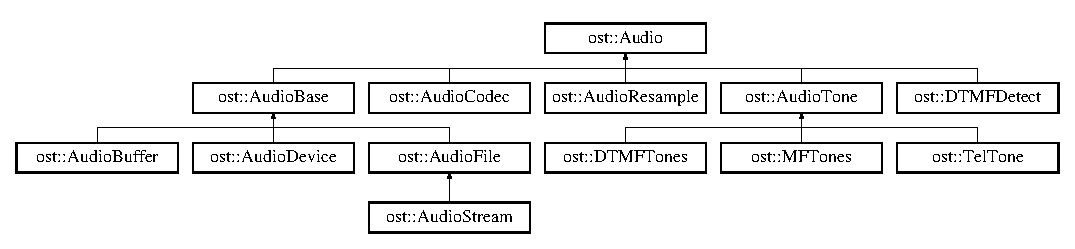
\includegraphics[height=2.89406cm]{classost_1_1_audio}
\end{center}
\end{figure}
\subsection*{Classes}
\begin{DoxyCompactItemize}
\item 
struct {\bf dtmf\_\-detect\_\-state\_\-t}
\item 
struct {\bf goertzel\_\-state\_\-t}
\item 
class {\bf Info}
\begin{DoxyCompactList}\small\item\em \doxyref{Audio}{p.}{classost_1_1_audio} source description. \item\end{DoxyCompactList}\item 
struct {\bf mpeg\_\-audio}
\item 
struct {\bf mpeg\_\-tagv1}
\item 
struct {\bf tone\_\-detection\_\-descriptor\_\-t}
\end{DoxyCompactItemize}
\subsection*{Public Types}
\begin{DoxyCompactItemize}
\item 
enum {\bf Rate} \{ \par
{\bf rateUnknown}, 
{\bf rate6khz} =  6000, 
{\bf rate8khz} =  8000, 
{\bf rate16khz} =  16000, 
\par
{\bf rate32khz} =  32000, 
{\bf rate44khz} =  44100
 \}
\begin{DoxyCompactList}\small\item\em \doxyref{Audio}{p.}{classost_1_1_audio} encoding rate, samples per second. \item\end{DoxyCompactList}\item 
enum {\bf Mode} \{ \par
{\bf modeRead}, 
{\bf modeReadAny}, 
{\bf modeReadOne}, 
{\bf modeWrite}, 
\par
{\bf modeCache}, 
{\bf modeInfo}, 
{\bf modeFeed}, 
{\bf modeAppend}, 
\par
{\bf modeCreate}
 \}
\begin{DoxyCompactList}\small\item\em File processing mode, whether to skip missing files, etc. \item\end{DoxyCompactList}\item 
enum {\bf Encoding} \{ \par
{\bf unknownEncoding} =  0, 
{\bf g721ADPCM}, 
{\bf g722Audio}, 
{\bf g722\_\-7bit}, 
\par
{\bf g722\_\-6bit}, 
{\bf g723\_\-2bit}, 
{\bf g723\_\-3bit}, 
{\bf g723\_\-5bit}, 
\par
{\bf gsmVoice}, 
{\bf msgsmVoice}, 
{\bf mulawAudio}, 
{\bf alawAudio}, 
\par
{\bf mp1Audio}, 
{\bf mp2Audio}, 
{\bf mp3Audio}, 
{\bf okiADPCM}, 
\par
{\bf voxADPCM}, 
{\bf sx73Voice}, 
{\bf sx96Voice}, 
{\bf cdaStereo}, 
\par
{\bf cdaMono}, 
{\bf pcm8Stereo}, 
{\bf pcm8Mono}, 
{\bf pcm16Stereo}, 
\par
{\bf pcm16Mono}, 
{\bf pcm32Stereo}, 
{\bf pcm32Mono}, 
{\bf speexVoice}, 
\par
{\bf speexAudio}, 
{\bf g729Audio}, 
{\bf ilbcAudio}, 
{\bf speexUltra}, 
\par
{\bf speexNarrow} =  speexVoice, 
{\bf speexWide} =  speexAudio, 
{\bf g723\_\-4bit} =  g721ADPCM
 \}
\begin{DoxyCompactList}\small\item\em \doxyref{Audio}{p.}{classost_1_1_audio} encoding formats. \item\end{DoxyCompactList}\item 
enum {\bf Format} \{ \par
{\bf raw}, 
{\bf snd}, 
{\bf riff}, 
{\bf mpeg}, 
\par
{\bf wave}
 \}
\begin{DoxyCompactList}\small\item\em \doxyref{Audio}{p.}{classost_1_1_audio} container file format. \item\end{DoxyCompactList}\item 
enum {\bf DeviceMode} \{ {\bf PLAY}, 
{\bf RECORD}, 
{\bf PLAYREC}
 \}
\begin{DoxyCompactList}\small\item\em \doxyref{Audio}{p.}{classost_1_1_audio} device access mode. \item\end{DoxyCompactList}\item 
enum {\bf Error} \{ \par
{\bf errSuccess} =  0, 
{\bf errReadLast}, 
{\bf errNotOpened}, 
{\bf errEndOfFile}, 
\par
{\bf errStartOfFile}, 
{\bf errRateInvalid}, 
{\bf errEncodingInvalid}, 
{\bf errReadInterrupt}, 
\par
{\bf errWriteInterrupt}, 
{\bf errReadFailure}, 
{\bf errWriteFailure}, 
{\bf errReadIncomplete}, 
\par
{\bf errWriteIncomplete}, 
{\bf errRequestInvalid}, 
{\bf errTOCFailed}, 
{\bf errStatFailed}, 
\par
{\bf errInvalidTrack}, 
{\bf errPlaybackFailed}, 
{\bf errNotPlaying}, 
{\bf errNoCodec}
 \}
\begin{DoxyCompactList}\small\item\em \doxyref{Audio}{p.}{classost_1_1_audio} error conditions. \item\end{DoxyCompactList}\item 
typedef int16\_\-t {\bf snd16\_\-t}
\item 
typedef int32\_\-t {\bf snd32\_\-t}
\item 
typedef int16\_\-t {\bf Level}
\item 
typedef int16\_\-t {\bf Sample}
\item 
typedef int16\_\-t $\ast$ {\bf Linear}
\item 
typedef unsigned long {\bf timeout\_\-t}
\item 
typedef unsigned char $\ast$ {\bf Encoded}
\item 
typedef enum {\bf Rate} {\bf Rate}
\item 
typedef enum {\bf Mode} {\bf Mode}
\item 
typedef enum {\bf Encoding} {\bf Encoding}
\item 
typedef enum {\bf Format} {\bf Format}
\item 
typedef enum {\bf DeviceMode} {\bf DeviceMode}
\item 
typedef enum {\bf Error} {\bf Error}
\end{DoxyCompactItemize}
\subsection*{Static Public Member Functions}
\begin{DoxyCompactItemize}
\item 
static {\bf Level} {\bf tolevel} (float dbm)
\begin{DoxyCompactList}\small\item\em Convert dbm power level to integer value (0-\/32768). \item\end{DoxyCompactList}\item 
static float {\bf todbm} ({\bf Level} power)
\begin{DoxyCompactList}\small\item\em Convert integer power levels to dbm. \item\end{DoxyCompactList}\item 
static bool {\bf hasDevice} (unsigned device=0)
\begin{DoxyCompactList}\small\item\em Test for the presense of a specified (indexed) audio device. \item\end{DoxyCompactList}\item 
static {\bf AudioDevice} $\ast$ {\bf getDevice} (unsigned device=0, {\bf DeviceMode} mode=PLAY)
\begin{DoxyCompactList}\small\item\em Get a audio device object that can be used to play or record audio. \item\end{DoxyCompactList}\item 
static const char $\ast$ {\bf getCodecPath} (void)
\begin{DoxyCompactList}\small\item\em Get pathname to where loadable codec modules are stored. \item\end{DoxyCompactList}\item 
static const char $\ast$ {\bf getMIME} ({\bf Info} \&info)
\begin{DoxyCompactList}\small\item\em Get the mime descriptive type for a given \doxyref{Audio}{p.}{classost_1_1_audio} encoding description, usually retrieved from a newly opened audio file. \item\end{DoxyCompactList}\item 
static const char $\ast$ {\bf getName} ({\bf Encoding} encoding)
\begin{DoxyCompactList}\small\item\em Get the short ascii description used for the given audio encoding type. \item\end{DoxyCompactList}\item 
static const char $\ast$ {\bf getExtension} ({\bf Encoding} encoding)
\begin{DoxyCompactList}\small\item\em Get the preferred file extension name to use for a given audio encoding type. \item\end{DoxyCompactList}\item 
static {\bf Encoding} {\bf getEncoding} (const char $\ast$name)
\begin{DoxyCompactList}\small\item\em Get the audio encoding format that is specified by a short ascii name. \item\end{DoxyCompactList}\item 
static {\bf Encoding} {\bf getStereo} ({\bf Encoding} encoding)
\begin{DoxyCompactList}\small\item\em Get the stereo encoding format associated with the given format. \item\end{DoxyCompactList}\item 
static {\bf Encoding} {\bf getMono} ({\bf Encoding} encoding)
\begin{DoxyCompactList}\small\item\em Get the mono encoding format associated with the given format. \item\end{DoxyCompactList}\item 
static bool {\bf isLinear} ({\bf Encoding} encoding)
\begin{DoxyCompactList}\small\item\em Test if the audio encoding format is a linear one. \item\end{DoxyCompactList}\item 
static bool {\bf isBuffered} ({\bf Encoding} encoding)
\begin{DoxyCompactList}\small\item\em Test if the audio encoding format must be packetized (that is, has irregular sized frames) and must be processed only through buffered codecs. \item\end{DoxyCompactList}\item 
static bool {\bf isMono} ({\bf Encoding} encoding)
\begin{DoxyCompactList}\small\item\em Test if the audio encoding format is a mono format. \item\end{DoxyCompactList}\item 
static bool {\bf isStereo} ({\bf Encoding} encoding)
\begin{DoxyCompactList}\small\item\em Test if the audio encoding format is a stereo format. \item\end{DoxyCompactList}\item 
static {\bf Rate} {\bf getRate} ({\bf Encoding} encoding)
\begin{DoxyCompactList}\small\item\em Return default sample rate associated with the specified audio encoding format. \item\end{DoxyCompactList}\item 
static {\bf Rate} {\bf getRate} ({\bf Encoding} e, {\bf Rate} request)
\begin{DoxyCompactList}\small\item\em Return optional rate setting effect. \item\end{DoxyCompactList}\item 
static {\bf timeout\_\-t} {\bf getFraming} ({\bf Encoding} encoding, {\bf timeout\_\-t} timeout=0)
\begin{DoxyCompactList}\small\item\em Return frame timing for an audio encoding format. \item\end{DoxyCompactList}\item 
static {\bf timeout\_\-t} {\bf getFraming} ({\bf Info} \&info, {\bf timeout\_\-t} timeout=0)
\begin{DoxyCompactList}\small\item\em Return frame time for an audio source description. \item\end{DoxyCompactList}\item 
static bool {\bf isEndian} ({\bf Encoding} encoding)
\begin{DoxyCompactList}\small\item\em Test if the endian byte order of the encoding format is different from the machine's native byte order. \item\end{DoxyCompactList}\item 
static bool {\bf isEndian} ({\bf Info} \&info)
\begin{DoxyCompactList}\small\item\em Test if the endian byte order of the audio source description is different from the machine's native byte order. \item\end{DoxyCompactList}\item 
static bool {\bf swapEndian} ({\bf Encoding} encoding, void $\ast$buffer, unsigned number)
\begin{DoxyCompactList}\small\item\em Optionally swap endian of audio data if the encoding format endian byte order is different from the machine's native endian. \item\end{DoxyCompactList}\item 
static void {\bf swapEncoded} ({\bf Info} \&info, {\bf Encoded} data, size\_\-t bytes)
\begin{DoxyCompactList}\small\item\em Optionally swap endian of encoded audio data based on the audio encoding type, and relationship to native byte order. \item\end{DoxyCompactList}\item 
static bool {\bf swapEndian} ({\bf Info} \&info, void $\ast$buffer, unsigned number)
\begin{DoxyCompactList}\small\item\em Optionally swap endian of audio data if the audio source description byte order is different from the machine's native endian byte order. \item\end{DoxyCompactList}\item 
static {\bf Level} {\bf getImpulse} ({\bf Encoding} encoding, void $\ast$buffer, unsigned number)
\begin{DoxyCompactList}\small\item\em Get the energey impulse level of a frame of audio data. \item\end{DoxyCompactList}\item 
static {\bf Level} {\bf getImpulse} ({\bf Info} \&info, void $\ast$buffer, unsigned number=0)
\begin{DoxyCompactList}\small\item\em Get the energey impulse level of a frame of audio data. \item\end{DoxyCompactList}\item 
static {\bf Level} {\bf getPeak} ({\bf Encoding} encoding, void $\ast$buffer, unsigned number)
\begin{DoxyCompactList}\small\item\em Get the peak (highest energy) level found in a frame of audio data. \item\end{DoxyCompactList}\item 
static {\bf Level} {\bf getPeak} ({\bf Info} \&info, void $\ast$buffer, unsigned number=0)
\begin{DoxyCompactList}\small\item\em Get the peak (highest energy) level found in a frame of audio data. \item\end{DoxyCompactList}\item 
static void {\bf toTimestamp} ({\bf timeout\_\-t} duration, char $\ast$address, size\_\-t size)
\begin{DoxyCompactList}\small\item\em Provide ascii timestamp representation of a timeout value. \item\end{DoxyCompactList}\item 
static {\bf timeout\_\-t} {\bf toTimeout} (const char $\ast$timestamp)
\begin{DoxyCompactList}\small\item\em Convert ascii timestamp representation to a timeout number. \item\end{DoxyCompactList}\item 
static int {\bf getFrame} ({\bf Encoding} encoding, int samples=0)
\begin{DoxyCompactList}\small\item\em Returns the number of bytes in a sample frame for the given encoding type, rounded up to the nearest integer. \item\end{DoxyCompactList}\item 
static int {\bf getCount} ({\bf Encoding} encoding)
\begin{DoxyCompactList}\small\item\em Returns the number of samples in all channels for a frame in the given encoding. \item\end{DoxyCompactList}\item 
static unsigned long {\bf toSamples} ({\bf Encoding} encoding, size\_\-t bytes)
\begin{DoxyCompactList}\small\item\em Compute byte counts of audio data into number of samples based on the audio encoding format used. \item\end{DoxyCompactList}\item 
static unsigned long {\bf toSamples} ({\bf Info} \&info, size\_\-t bytes)
\begin{DoxyCompactList}\small\item\em Compute byte counts of audio data into number of samples based on the audio source description used. \item\end{DoxyCompactList}\item 
static size\_\-t {\bf toBytes} ({\bf Info} \&info, unsigned long number)
\begin{DoxyCompactList}\small\item\em Compute the number of bytes a given number of samples in a given audio encoding will occupy. \item\end{DoxyCompactList}\item 
static size\_\-t {\bf toBytes} ({\bf Encoding} encoding, unsigned long number)
\begin{DoxyCompactList}\small\item\em Compute the number of bytes a given number of samples in a given audio encoding will occupy. \item\end{DoxyCompactList}\item 
static void {\bf fill} (unsigned char $\ast$address, int number, {\bf Encoding} encoding)
\begin{DoxyCompactList}\small\item\em Fill an audio buffer with \char`\"{}empty\char`\"{} (silent) audio data, based on the audio encoding format. \item\end{DoxyCompactList}\item 
static bool {\bf loadPlugin} (const char $\ast$path)
\begin{DoxyCompactList}\small\item\em Load a dso plugin (codec plugin), used internally. \item\end{DoxyCompactList}\item 
static size\_\-t {\bf maxFramesize} ({\bf Info} \&info)
\begin{DoxyCompactList}\small\item\em Maximum framesize for a given coding that may be needed to store a result. \item\end{DoxyCompactList}\end{DoxyCompactItemize}
\subsection*{Static Public Attributes}
\begin{DoxyCompactItemize}
\item 
static const unsigned {\bf ndata}
\end{DoxyCompactItemize}


\subsection{Detailed Description}
Generic audio class to hold master data types and various useful class encapsulated friend functions as per GNU Common C++ 2 coding standard. \begin{DoxyAuthor}{Author}
David Sugar $<${\tt dyfet@ostel.com}$>$ Master audio class. 
\end{DoxyAuthor}


\subsection{Member Typedef Documentation}
\index{ost::Audio@{ost::Audio}!DeviceMode@{DeviceMode}}
\index{DeviceMode@{DeviceMode}!ost::Audio@{ost::Audio}}
\subsubsection[{DeviceMode}]{\setlength{\rightskip}{0pt plus 5cm}typedef enum {\bf DeviceMode} {\bf ost::Audio::DeviceMode}}\label{classost_1_1_audio_a64ea45fd7b796a2de14093e69591bbc1}
\index{ost::Audio@{ost::Audio}!Encoded@{Encoded}}
\index{Encoded@{Encoded}!ost::Audio@{ost::Audio}}
\subsubsection[{Encoded}]{\setlength{\rightskip}{0pt plus 5cm}typedef unsigned char$\ast$ {\bf ost::Audio::Encoded}}\label{classost_1_1_audio_a5c7e49d2b98c74b5a63a0e52a31e626e}
\index{ost::Audio@{ost::Audio}!Encoding@{Encoding}}
\index{Encoding@{Encoding}!ost::Audio@{ost::Audio}}
\subsubsection[{Encoding}]{\setlength{\rightskip}{0pt plus 5cm}typedef enum {\bf Encoding} {\bf ost::Audio::Encoding}}\label{classost_1_1_audio_ac6a37d56c55e4e90c76e1ff32c5a9b4d}
\index{ost::Audio@{ost::Audio}!Error@{Error}}
\index{Error@{Error}!ost::Audio@{ost::Audio}}
\subsubsection[{Error}]{\setlength{\rightskip}{0pt plus 5cm}typedef enum {\bf Error} {\bf ost::Audio::Error}}\label{classost_1_1_audio_afc24bc71c6ce0c97f0c349291eed74cf}
\index{ost::Audio@{ost::Audio}!Format@{Format}}
\index{Format@{Format}!ost::Audio@{ost::Audio}}
\subsubsection[{Format}]{\setlength{\rightskip}{0pt plus 5cm}typedef enum {\bf Format} {\bf ost::Audio::Format}}\label{classost_1_1_audio_a10021256123af9a4b31bf1f69629524c}
\index{ost::Audio@{ost::Audio}!Level@{Level}}
\index{Level@{Level}!ost::Audio@{ost::Audio}}
\subsubsection[{Level}]{\setlength{\rightskip}{0pt plus 5cm}typedef int16\_\-t {\bf ost::Audio::Level}}\label{classost_1_1_audio_a4dda00f9d98568cf340f94e9bd0fcd88}
\index{ost::Audio@{ost::Audio}!Linear@{Linear}}
\index{Linear@{Linear}!ost::Audio@{ost::Audio}}
\subsubsection[{Linear}]{\setlength{\rightskip}{0pt plus 5cm}typedef int16\_\-t$\ast$ {\bf ost::Audio::Linear}}\label{classost_1_1_audio_a8e557e78d8d049df8f2ed5eb0b60cea9}
\index{ost::Audio@{ost::Audio}!Mode@{Mode}}
\index{Mode@{Mode}!ost::Audio@{ost::Audio}}
\subsubsection[{Mode}]{\setlength{\rightskip}{0pt plus 5cm}typedef enum {\bf Mode} {\bf ost::Audio::Mode}}\label{classost_1_1_audio_aaa5de3c7b74ee304a5292d79a6a4df9b}
\index{ost::Audio@{ost::Audio}!Rate@{Rate}}
\index{Rate@{Rate}!ost::Audio@{ost::Audio}}
\subsubsection[{Rate}]{\setlength{\rightskip}{0pt plus 5cm}typedef enum {\bf Rate} {\bf ost::Audio::Rate}}\label{classost_1_1_audio_af100e5274ac000c170299e83b87a1314}
\index{ost::Audio@{ost::Audio}!Sample@{Sample}}
\index{Sample@{Sample}!ost::Audio@{ost::Audio}}
\subsubsection[{Sample}]{\setlength{\rightskip}{0pt plus 5cm}typedef int16\_\-t {\bf ost::Audio::Sample}}\label{classost_1_1_audio_ab9d6b2f16d237f7c70a6ea783fce52f6}
\index{ost::Audio@{ost::Audio}!snd16\_\-t@{snd16\_\-t}}
\index{snd16\_\-t@{snd16\_\-t}!ost::Audio@{ost::Audio}}
\subsubsection[{snd16\_\-t}]{\setlength{\rightskip}{0pt plus 5cm}typedef int16\_\-t {\bf ost::Audio::snd16\_\-t}}\label{classost_1_1_audio_a1b3506ec0126f95fe8f4eadd7d79b6da}
\index{ost::Audio@{ost::Audio}!snd32\_\-t@{snd32\_\-t}}
\index{snd32\_\-t@{snd32\_\-t}!ost::Audio@{ost::Audio}}
\subsubsection[{snd32\_\-t}]{\setlength{\rightskip}{0pt plus 5cm}typedef int32\_\-t {\bf ost::Audio::snd32\_\-t}}\label{classost_1_1_audio_a121b4a42005124b043b33cc6e7bb374e}
\index{ost::Audio@{ost::Audio}!timeout\_\-t@{timeout\_\-t}}
\index{timeout\_\-t@{timeout\_\-t}!ost::Audio@{ost::Audio}}
\subsubsection[{timeout\_\-t}]{\setlength{\rightskip}{0pt plus 5cm}typedef unsigned long {\bf ost::Audio::timeout\_\-t}}\label{classost_1_1_audio_adaaf1ff03bfae21e5d6231b2f944b490}


\subsection{Member Enumeration Documentation}
\index{ost::Audio@{ost::Audio}!DeviceMode@{DeviceMode}}
\index{DeviceMode@{DeviceMode}!ost::Audio@{ost::Audio}}
\subsubsection[{DeviceMode}]{\setlength{\rightskip}{0pt plus 5cm}enum {\bf ost::Audio::DeviceMode}}\label{classost_1_1_audio_a6ed0d85bd28cabe648d18832e54777c1}


\doxyref{Audio}{p.}{classost_1_1_audio} device access mode. \begin{Desc}
\item[Enumerator: ]\par
\begin{description}
\index{PLAY@{PLAY}!ost::Audio@{ost::Audio}}\index{ost::Audio@{ost::Audio}!PLAY@{PLAY}}\item[{\em 
PLAY\label{classost_1_1_audio_a6ed0d85bd28cabe648d18832e54777c1a434fa31ee9406fe04ab7d39359f5d5b5}
}]\index{RECORD@{RECORD}!ost::Audio@{ost::Audio}}\index{ost::Audio@{ost::Audio}!RECORD@{RECORD}}\item[{\em 
RECORD\label{classost_1_1_audio_a6ed0d85bd28cabe648d18832e54777c1a859407d0f38e9b07ac7ea646f21b2114}
}]\index{PLAYREC@{PLAYREC}!ost::Audio@{ost::Audio}}\index{ost::Audio@{ost::Audio}!PLAYREC@{PLAYREC}}\item[{\em 
PLAYREC\label{classost_1_1_audio_a6ed0d85bd28cabe648d18832e54777c1a2a5f699cdda2e8e061f9630069505c58}
}]\end{description}
\end{Desc}

\index{ost::Audio@{ost::Audio}!Encoding@{Encoding}}
\index{Encoding@{Encoding}!ost::Audio@{ost::Audio}}
\subsubsection[{Encoding}]{\setlength{\rightskip}{0pt plus 5cm}enum {\bf ost::Audio::Encoding}}\label{classost_1_1_audio_ac000fdc6e71fc298896e5060e1e331ba}


\doxyref{Audio}{p.}{classost_1_1_audio} encoding formats. \begin{Desc}
\item[Enumerator: ]\par
\begin{description}
\index{unknownEncoding@{unknownEncoding}!ost::Audio@{ost::Audio}}\index{ost::Audio@{ost::Audio}!unknownEncoding@{unknownEncoding}}\item[{\em 
unknownEncoding\label{classost_1_1_audio_ac000fdc6e71fc298896e5060e1e331baa8e09e897a62d7a5ecc3dce9282619883}
}]\index{g721ADPCM@{g721ADPCM}!ost::Audio@{ost::Audio}}\index{ost::Audio@{ost::Audio}!g721ADPCM@{g721ADPCM}}\item[{\em 
g721ADPCM\label{classost_1_1_audio_ac000fdc6e71fc298896e5060e1e331baa9aee334a2d893ad44d7a3856e87a34a0}
}]\index{g722Audio@{g722Audio}!ost::Audio@{ost::Audio}}\index{ost::Audio@{ost::Audio}!g722Audio@{g722Audio}}\item[{\em 
g722Audio\label{classost_1_1_audio_ac000fdc6e71fc298896e5060e1e331baa0128360769248d7ebbc61bb1bdea060f}
}]\index{g722\_\-7bit@{g722\_\-7bit}!ost::Audio@{ost::Audio}}\index{ost::Audio@{ost::Audio}!g722\_\-7bit@{g722\_\-7bit}}\item[{\em 
g722\_\-7bit\label{classost_1_1_audio_ac000fdc6e71fc298896e5060e1e331baa9bad14942804ae774da37c17ebf1c5a2}
}]\index{g722\_\-6bit@{g722\_\-6bit}!ost::Audio@{ost::Audio}}\index{ost::Audio@{ost::Audio}!g722\_\-6bit@{g722\_\-6bit}}\item[{\em 
g722\_\-6bit\label{classost_1_1_audio_ac000fdc6e71fc298896e5060e1e331baa3f2c9e61b4a788f8e2ddabea3e0e64a5}
}]\index{g723\_\-2bit@{g723\_\-2bit}!ost::Audio@{ost::Audio}}\index{ost::Audio@{ost::Audio}!g723\_\-2bit@{g723\_\-2bit}}\item[{\em 
g723\_\-2bit\label{classost_1_1_audio_ac000fdc6e71fc298896e5060e1e331baaaa50db3a491cbd7a56e2ca9519216c31}
}]\index{g723\_\-3bit@{g723\_\-3bit}!ost::Audio@{ost::Audio}}\index{ost::Audio@{ost::Audio}!g723\_\-3bit@{g723\_\-3bit}}\item[{\em 
g723\_\-3bit\label{classost_1_1_audio_ac000fdc6e71fc298896e5060e1e331baa232c38a80a6707ffa9c40a0ebce849d2}
}]\index{g723\_\-5bit@{g723\_\-5bit}!ost::Audio@{ost::Audio}}\index{ost::Audio@{ost::Audio}!g723\_\-5bit@{g723\_\-5bit}}\item[{\em 
g723\_\-5bit\label{classost_1_1_audio_ac000fdc6e71fc298896e5060e1e331baac33334f21056ca768c932faa58ee4e3b}
}]\index{gsmVoice@{gsmVoice}!ost::Audio@{ost::Audio}}\index{ost::Audio@{ost::Audio}!gsmVoice@{gsmVoice}}\item[{\em 
gsmVoice\label{classost_1_1_audio_ac000fdc6e71fc298896e5060e1e331baa8ad54db389dbd71a73db82bc44457d95}
}]\index{msgsmVoice@{msgsmVoice}!ost::Audio@{ost::Audio}}\index{ost::Audio@{ost::Audio}!msgsmVoice@{msgsmVoice}}\item[{\em 
msgsmVoice\label{classost_1_1_audio_ac000fdc6e71fc298896e5060e1e331baa9c776ce70f0499bb61b8954b74a8fac7}
}]\index{mulawAudio@{mulawAudio}!ost::Audio@{ost::Audio}}\index{ost::Audio@{ost::Audio}!mulawAudio@{mulawAudio}}\item[{\em 
mulawAudio\label{classost_1_1_audio_ac000fdc6e71fc298896e5060e1e331baa5f6c81d40b3bb2e78e7fbc30fdbd2074}
}]\index{alawAudio@{alawAudio}!ost::Audio@{ost::Audio}}\index{ost::Audio@{ost::Audio}!alawAudio@{alawAudio}}\item[{\em 
alawAudio\label{classost_1_1_audio_ac000fdc6e71fc298896e5060e1e331baa72609cc1ee8752337012b27f8c63d016}
}]\index{mp1Audio@{mp1Audio}!ost::Audio@{ost::Audio}}\index{ost::Audio@{ost::Audio}!mp1Audio@{mp1Audio}}\item[{\em 
mp1Audio\label{classost_1_1_audio_ac000fdc6e71fc298896e5060e1e331baa04a05a2df746a4d72e35571b67cc5284}
}]\index{mp2Audio@{mp2Audio}!ost::Audio@{ost::Audio}}\index{ost::Audio@{ost::Audio}!mp2Audio@{mp2Audio}}\item[{\em 
mp2Audio\label{classost_1_1_audio_ac000fdc6e71fc298896e5060e1e331baa89cb4e37330a69f5e180ddb463d7740e}
}]\index{mp3Audio@{mp3Audio}!ost::Audio@{ost::Audio}}\index{ost::Audio@{ost::Audio}!mp3Audio@{mp3Audio}}\item[{\em 
mp3Audio\label{classost_1_1_audio_ac000fdc6e71fc298896e5060e1e331baa56d99d68ada26ec7dd4f53414461badd}
}]\index{okiADPCM@{okiADPCM}!ost::Audio@{ost::Audio}}\index{ost::Audio@{ost::Audio}!okiADPCM@{okiADPCM}}\item[{\em 
okiADPCM\label{classost_1_1_audio_ac000fdc6e71fc298896e5060e1e331baaa4e009edc72290cc7e375c54a66e17a6}
}]\index{voxADPCM@{voxADPCM}!ost::Audio@{ost::Audio}}\index{ost::Audio@{ost::Audio}!voxADPCM@{voxADPCM}}\item[{\em 
voxADPCM\label{classost_1_1_audio_ac000fdc6e71fc298896e5060e1e331baaae3709b42ebf20e118b3d8dbe7d8996b}
}]\index{sx73Voice@{sx73Voice}!ost::Audio@{ost::Audio}}\index{ost::Audio@{ost::Audio}!sx73Voice@{sx73Voice}}\item[{\em 
sx73Voice\label{classost_1_1_audio_ac000fdc6e71fc298896e5060e1e331baa2d14662303292d014327a93f6ac68802}
}]\index{sx96Voice@{sx96Voice}!ost::Audio@{ost::Audio}}\index{ost::Audio@{ost::Audio}!sx96Voice@{sx96Voice}}\item[{\em 
sx96Voice\label{classost_1_1_audio_ac000fdc6e71fc298896e5060e1e331baab7d3a16e18d1b00bb56d91843d8fe2b8}
}]\index{cdaStereo@{cdaStereo}!ost::Audio@{ost::Audio}}\index{ost::Audio@{ost::Audio}!cdaStereo@{cdaStereo}}\item[{\em 
cdaStereo\label{classost_1_1_audio_ac000fdc6e71fc298896e5060e1e331baa5ca72fd2aa7204223dd90d25b361fbf6}
}]\index{cdaMono@{cdaMono}!ost::Audio@{ost::Audio}}\index{ost::Audio@{ost::Audio}!cdaMono@{cdaMono}}\item[{\em 
cdaMono\label{classost_1_1_audio_ac000fdc6e71fc298896e5060e1e331baa21542716b78d850f6ffe02bbbac160ec}
}]\index{pcm8Stereo@{pcm8Stereo}!ost::Audio@{ost::Audio}}\index{ost::Audio@{ost::Audio}!pcm8Stereo@{pcm8Stereo}}\item[{\em 
pcm8Stereo\label{classost_1_1_audio_ac000fdc6e71fc298896e5060e1e331baa6361df110128c2e5b774c9bf1496b102}
}]\index{pcm8Mono@{pcm8Mono}!ost::Audio@{ost::Audio}}\index{ost::Audio@{ost::Audio}!pcm8Mono@{pcm8Mono}}\item[{\em 
pcm8Mono\label{classost_1_1_audio_ac000fdc6e71fc298896e5060e1e331baae163dd3eddff63ed6a184fb21461b330}
}]\index{pcm16Stereo@{pcm16Stereo}!ost::Audio@{ost::Audio}}\index{ost::Audio@{ost::Audio}!pcm16Stereo@{pcm16Stereo}}\item[{\em 
pcm16Stereo\label{classost_1_1_audio_ac000fdc6e71fc298896e5060e1e331baaaecacf9d126404dee63f19df016ed8a2}
}]\index{pcm16Mono@{pcm16Mono}!ost::Audio@{ost::Audio}}\index{ost::Audio@{ost::Audio}!pcm16Mono@{pcm16Mono}}\item[{\em 
pcm16Mono\label{classost_1_1_audio_ac000fdc6e71fc298896e5060e1e331baac8d2724c58b6015260e1eeafe4045baa}
}]\index{pcm32Stereo@{pcm32Stereo}!ost::Audio@{ost::Audio}}\index{ost::Audio@{ost::Audio}!pcm32Stereo@{pcm32Stereo}}\item[{\em 
pcm32Stereo\label{classost_1_1_audio_ac000fdc6e71fc298896e5060e1e331baa689c16b1c20517c6e6b4d5a1877ef677}
}]\index{pcm32Mono@{pcm32Mono}!ost::Audio@{ost::Audio}}\index{ost::Audio@{ost::Audio}!pcm32Mono@{pcm32Mono}}\item[{\em 
pcm32Mono\label{classost_1_1_audio_ac000fdc6e71fc298896e5060e1e331baa5d5349654c1f97010f3a1a722d49aa68}
}]\index{speexVoice@{speexVoice}!ost::Audio@{ost::Audio}}\index{ost::Audio@{ost::Audio}!speexVoice@{speexVoice}}\item[{\em 
speexVoice\label{classost_1_1_audio_ac000fdc6e71fc298896e5060e1e331baa5c1b17694150aa7c8cb33fb2e3a78cb7}
}]\index{speexAudio@{speexAudio}!ost::Audio@{ost::Audio}}\index{ost::Audio@{ost::Audio}!speexAudio@{speexAudio}}\item[{\em 
speexAudio\label{classost_1_1_audio_ac000fdc6e71fc298896e5060e1e331baa731f9bb579ecbb50b663970a2f504a49}
}]\index{g729Audio@{g729Audio}!ost::Audio@{ost::Audio}}\index{ost::Audio@{ost::Audio}!g729Audio@{g729Audio}}\item[{\em 
g729Audio\label{classost_1_1_audio_ac000fdc6e71fc298896e5060e1e331baa18a9a174c23c51a90fd1043bb2c5b1b1}
}]\index{ilbcAudio@{ilbcAudio}!ost::Audio@{ost::Audio}}\index{ost::Audio@{ost::Audio}!ilbcAudio@{ilbcAudio}}\item[{\em 
ilbcAudio\label{classost_1_1_audio_ac000fdc6e71fc298896e5060e1e331baaf9096458bb864e2c7003c1c61d18adc4}
}]\index{speexUltra@{speexUltra}!ost::Audio@{ost::Audio}}\index{ost::Audio@{ost::Audio}!speexUltra@{speexUltra}}\item[{\em 
speexUltra\label{classost_1_1_audio_ac000fdc6e71fc298896e5060e1e331baa0c6336bb14ee0129e8e1f97b276cada0}
}]\index{speexNarrow@{speexNarrow}!ost::Audio@{ost::Audio}}\index{ost::Audio@{ost::Audio}!speexNarrow@{speexNarrow}}\item[{\em 
speexNarrow\label{classost_1_1_audio_ac000fdc6e71fc298896e5060e1e331baa29abde2c5d8761d855a19f377d280bd3}
}]\index{speexWide@{speexWide}!ost::Audio@{ost::Audio}}\index{ost::Audio@{ost::Audio}!speexWide@{speexWide}}\item[{\em 
speexWide\label{classost_1_1_audio_ac000fdc6e71fc298896e5060e1e331baafbdfc0c366fd02319cdc026e7ae9a67f}
}]\index{g723\_\-4bit@{g723\_\-4bit}!ost::Audio@{ost::Audio}}\index{ost::Audio@{ost::Audio}!g723\_\-4bit@{g723\_\-4bit}}\item[{\em 
g723\_\-4bit\label{classost_1_1_audio_ac000fdc6e71fc298896e5060e1e331baa80f1c4463d696f269587e60ccb62a137}
}]\end{description}
\end{Desc}

\index{ost::Audio@{ost::Audio}!Error@{Error}}
\index{Error@{Error}!ost::Audio@{ost::Audio}}
\subsubsection[{Error}]{\setlength{\rightskip}{0pt plus 5cm}enum {\bf ost::Audio::Error}}\label{classost_1_1_audio_a9b399c8c40f1c9c460490efeb3f86884}


\doxyref{Audio}{p.}{classost_1_1_audio} error conditions. \begin{Desc}
\item[Enumerator: ]\par
\begin{description}
\index{errSuccess@{errSuccess}!ost::Audio@{ost::Audio}}\index{ost::Audio@{ost::Audio}!errSuccess@{errSuccess}}\item[{\em 
errSuccess\label{classost_1_1_audio_a9b399c8c40f1c9c460490efeb3f86884aaf27439b02b8237b6a56c822f180414d}
}]\index{errReadLast@{errReadLast}!ost::Audio@{ost::Audio}}\index{ost::Audio@{ost::Audio}!errReadLast@{errReadLast}}\item[{\em 
errReadLast\label{classost_1_1_audio_a9b399c8c40f1c9c460490efeb3f86884af0b6200842a9819e841ed6483b073da3}
}]\index{errNotOpened@{errNotOpened}!ost::Audio@{ost::Audio}}\index{ost::Audio@{ost::Audio}!errNotOpened@{errNotOpened}}\item[{\em 
errNotOpened\label{classost_1_1_audio_a9b399c8c40f1c9c460490efeb3f86884a234d5e01216dd2709e1a302178e2b769}
}]\index{errEndOfFile@{errEndOfFile}!ost::Audio@{ost::Audio}}\index{ost::Audio@{ost::Audio}!errEndOfFile@{errEndOfFile}}\item[{\em 
errEndOfFile\label{classost_1_1_audio_a9b399c8c40f1c9c460490efeb3f86884a3893553d65303314f79536b41ca3d15e}
}]\index{errStartOfFile@{errStartOfFile}!ost::Audio@{ost::Audio}}\index{ost::Audio@{ost::Audio}!errStartOfFile@{errStartOfFile}}\item[{\em 
errStartOfFile\label{classost_1_1_audio_a9b399c8c40f1c9c460490efeb3f86884a2d8e975e5200165280499b9604b98212}
}]\index{errRateInvalid@{errRateInvalid}!ost::Audio@{ost::Audio}}\index{ost::Audio@{ost::Audio}!errRateInvalid@{errRateInvalid}}\item[{\em 
errRateInvalid\label{classost_1_1_audio_a9b399c8c40f1c9c460490efeb3f86884a0a06eeec844e19cd445213bbdf20f0a1}
}]\index{errEncodingInvalid@{errEncodingInvalid}!ost::Audio@{ost::Audio}}\index{ost::Audio@{ost::Audio}!errEncodingInvalid@{errEncodingInvalid}}\item[{\em 
errEncodingInvalid\label{classost_1_1_audio_a9b399c8c40f1c9c460490efeb3f86884a090ca64e7dfece97811c37bd076937da}
}]\index{errReadInterrupt@{errReadInterrupt}!ost::Audio@{ost::Audio}}\index{ost::Audio@{ost::Audio}!errReadInterrupt@{errReadInterrupt}}\item[{\em 
errReadInterrupt\label{classost_1_1_audio_a9b399c8c40f1c9c460490efeb3f86884a90fe70ebd883cafe2f647c3eb7b0aa37}
}]\index{errWriteInterrupt@{errWriteInterrupt}!ost::Audio@{ost::Audio}}\index{ost::Audio@{ost::Audio}!errWriteInterrupt@{errWriteInterrupt}}\item[{\em 
errWriteInterrupt\label{classost_1_1_audio_a9b399c8c40f1c9c460490efeb3f86884a156cc653457d3f76935b7f8bc856d43f}
}]\index{errReadFailure@{errReadFailure}!ost::Audio@{ost::Audio}}\index{ost::Audio@{ost::Audio}!errReadFailure@{errReadFailure}}\item[{\em 
errReadFailure\label{classost_1_1_audio_a9b399c8c40f1c9c460490efeb3f86884a0b98c4e843ad5feca37c2fcd2a960d48}
}]\index{errWriteFailure@{errWriteFailure}!ost::Audio@{ost::Audio}}\index{ost::Audio@{ost::Audio}!errWriteFailure@{errWriteFailure}}\item[{\em 
errWriteFailure\label{classost_1_1_audio_a9b399c8c40f1c9c460490efeb3f86884a73662d71bc5ac2b5df735ef7a95a04b9}
}]\index{errReadIncomplete@{errReadIncomplete}!ost::Audio@{ost::Audio}}\index{ost::Audio@{ost::Audio}!errReadIncomplete@{errReadIncomplete}}\item[{\em 
errReadIncomplete\label{classost_1_1_audio_a9b399c8c40f1c9c460490efeb3f86884ac51b3f3746de6f218335d8f9bd6edc17}
}]\index{errWriteIncomplete@{errWriteIncomplete}!ost::Audio@{ost::Audio}}\index{ost::Audio@{ost::Audio}!errWriteIncomplete@{errWriteIncomplete}}\item[{\em 
errWriteIncomplete\label{classost_1_1_audio_a9b399c8c40f1c9c460490efeb3f86884a7cdee9c419aa5ffaa8436f34da734c8e}
}]\index{errRequestInvalid@{errRequestInvalid}!ost::Audio@{ost::Audio}}\index{ost::Audio@{ost::Audio}!errRequestInvalid@{errRequestInvalid}}\item[{\em 
errRequestInvalid\label{classost_1_1_audio_a9b399c8c40f1c9c460490efeb3f86884a25186756cddbe09668774d34910c6054}
}]\index{errTOCFailed@{errTOCFailed}!ost::Audio@{ost::Audio}}\index{ost::Audio@{ost::Audio}!errTOCFailed@{errTOCFailed}}\item[{\em 
errTOCFailed\label{classost_1_1_audio_a9b399c8c40f1c9c460490efeb3f86884ad06c70265582cee5b91e93d75b4f5001}
}]\index{errStatFailed@{errStatFailed}!ost::Audio@{ost::Audio}}\index{ost::Audio@{ost::Audio}!errStatFailed@{errStatFailed}}\item[{\em 
errStatFailed\label{classost_1_1_audio_a9b399c8c40f1c9c460490efeb3f86884ad1b9591fb7b7d30ddad63f6e706bbaae}
}]\index{errInvalidTrack@{errInvalidTrack}!ost::Audio@{ost::Audio}}\index{ost::Audio@{ost::Audio}!errInvalidTrack@{errInvalidTrack}}\item[{\em 
errInvalidTrack\label{classost_1_1_audio_a9b399c8c40f1c9c460490efeb3f86884a88933ebeecc847bdd457c73bfa340a5c}
}]\index{errPlaybackFailed@{errPlaybackFailed}!ost::Audio@{ost::Audio}}\index{ost::Audio@{ost::Audio}!errPlaybackFailed@{errPlaybackFailed}}\item[{\em 
errPlaybackFailed\label{classost_1_1_audio_a9b399c8c40f1c9c460490efeb3f86884ab8f14090a0ce6e7df5ab0733d1d052be}
}]\index{errNotPlaying@{errNotPlaying}!ost::Audio@{ost::Audio}}\index{ost::Audio@{ost::Audio}!errNotPlaying@{errNotPlaying}}\item[{\em 
errNotPlaying\label{classost_1_1_audio_a9b399c8c40f1c9c460490efeb3f86884a34f559f52d6302c22ac2378815888d3e}
}]\index{errNoCodec@{errNoCodec}!ost::Audio@{ost::Audio}}\index{ost::Audio@{ost::Audio}!errNoCodec@{errNoCodec}}\item[{\em 
errNoCodec\label{classost_1_1_audio_a9b399c8c40f1c9c460490efeb3f86884a1491cc7eab3e1e461eb497552a5cadbf}
}]\end{description}
\end{Desc}

\index{ost::Audio@{ost::Audio}!Format@{Format}}
\index{Format@{Format}!ost::Audio@{ost::Audio}}
\subsubsection[{Format}]{\setlength{\rightskip}{0pt plus 5cm}enum {\bf ost::Audio::Format}}\label{classost_1_1_audio_a1b1f99ba120876f87870b8f7f007e924}


\doxyref{Audio}{p.}{classost_1_1_audio} container file format. \begin{Desc}
\item[Enumerator: ]\par
\begin{description}
\index{raw@{raw}!ost::Audio@{ost::Audio}}\index{ost::Audio@{ost::Audio}!raw@{raw}}\item[{\em 
raw\label{classost_1_1_audio_a1b1f99ba120876f87870b8f7f007e924ae71df2f88ae93b3040e400fc5beb6c1f}
}]\index{snd@{snd}!ost::Audio@{ost::Audio}}\index{ost::Audio@{ost::Audio}!snd@{snd}}\item[{\em 
snd\label{classost_1_1_audio_a1b1f99ba120876f87870b8f7f007e924a034a7bf5ce1cdb7990bff5260293241c}
}]\index{riff@{riff}!ost::Audio@{ost::Audio}}\index{ost::Audio@{ost::Audio}!riff@{riff}}\item[{\em 
riff\label{classost_1_1_audio_a1b1f99ba120876f87870b8f7f007e924aa8667be9bacfd6ed992b93191d88e17a}
}]\index{mpeg@{mpeg}!ost::Audio@{ost::Audio}}\index{ost::Audio@{ost::Audio}!mpeg@{mpeg}}\item[{\em 
mpeg\label{classost_1_1_audio_a1b1f99ba120876f87870b8f7f007e924a8a308f2000da135db008c71462ec16d5}
}]\index{wave@{wave}!ost::Audio@{ost::Audio}}\index{ost::Audio@{ost::Audio}!wave@{wave}}\item[{\em 
wave\label{classost_1_1_audio_a1b1f99ba120876f87870b8f7f007e924a932ca85af7639cd6db3f55534b1063eb}
}]\end{description}
\end{Desc}

\index{ost::Audio@{ost::Audio}!Mode@{Mode}}
\index{Mode@{Mode}!ost::Audio@{ost::Audio}}
\subsubsection[{Mode}]{\setlength{\rightskip}{0pt plus 5cm}enum {\bf ost::Audio::Mode}}\label{classost_1_1_audio_aaa0dde6cbf61934fcb527661a491ed5c}


File processing mode, whether to skip missing files, etc. \begin{Desc}
\item[Enumerator: ]\par
\begin{description}
\index{modeRead@{modeRead}!ost::Audio@{ost::Audio}}\index{ost::Audio@{ost::Audio}!modeRead@{modeRead}}\item[{\em 
modeRead\label{classost_1_1_audio_aaa0dde6cbf61934fcb527661a491ed5caecb1664beec2b86c5d87d86f64d0a84d}
}]\index{modeReadAny@{modeReadAny}!ost::Audio@{ost::Audio}}\index{ost::Audio@{ost::Audio}!modeReadAny@{modeReadAny}}\item[{\em 
modeReadAny\label{classost_1_1_audio_aaa0dde6cbf61934fcb527661a491ed5ca375f4b87b508327185bd6f19025b1424}
}]\index{modeReadOne@{modeReadOne}!ost::Audio@{ost::Audio}}\index{ost::Audio@{ost::Audio}!modeReadOne@{modeReadOne}}\item[{\em 
modeReadOne\label{classost_1_1_audio_aaa0dde6cbf61934fcb527661a491ed5ca58966349b002a4412997e2f141976273}
}]\index{modeWrite@{modeWrite}!ost::Audio@{ost::Audio}}\index{ost::Audio@{ost::Audio}!modeWrite@{modeWrite}}\item[{\em 
modeWrite\label{classost_1_1_audio_aaa0dde6cbf61934fcb527661a491ed5ca6f74b25c50c34c027a0720dd7dc32386}
}]\index{modeCache@{modeCache}!ost::Audio@{ost::Audio}}\index{ost::Audio@{ost::Audio}!modeCache@{modeCache}}\item[{\em 
modeCache\label{classost_1_1_audio_aaa0dde6cbf61934fcb527661a491ed5caf41875f19de18f05fc1c420a8d21f7c6}
}]\index{modeInfo@{modeInfo}!ost::Audio@{ost::Audio}}\index{ost::Audio@{ost::Audio}!modeInfo@{modeInfo}}\item[{\em 
modeInfo\label{classost_1_1_audio_aaa0dde6cbf61934fcb527661a491ed5caed372135c7f2d5e51e80d60f9d15a368}
}]\index{modeFeed@{modeFeed}!ost::Audio@{ost::Audio}}\index{ost::Audio@{ost::Audio}!modeFeed@{modeFeed}}\item[{\em 
modeFeed\label{classost_1_1_audio_aaa0dde6cbf61934fcb527661a491ed5caa955eac8a565410a7552fd7938cf2583}
}]\index{modeAppend@{modeAppend}!ost::Audio@{ost::Audio}}\index{ost::Audio@{ost::Audio}!modeAppend@{modeAppend}}\item[{\em 
modeAppend\label{classost_1_1_audio_aaa0dde6cbf61934fcb527661a491ed5caa320fddf63b1c9600aef25b47870e8c6}
}]\index{modeCreate@{modeCreate}!ost::Audio@{ost::Audio}}\index{ost::Audio@{ost::Audio}!modeCreate@{modeCreate}}\item[{\em 
modeCreate\label{classost_1_1_audio_aaa0dde6cbf61934fcb527661a491ed5ca47ed2d6bafa7f3495c8515625f96fe29}
}]\end{description}
\end{Desc}

\index{ost::Audio@{ost::Audio}!Rate@{Rate}}
\index{Rate@{Rate}!ost::Audio@{ost::Audio}}
\subsubsection[{Rate}]{\setlength{\rightskip}{0pt plus 5cm}enum {\bf ost::Audio::Rate}}\label{classost_1_1_audio_a38b5dfd1b29f5fd1acff3273582d18ed}


\doxyref{Audio}{p.}{classost_1_1_audio} encoding rate, samples per second. \begin{Desc}
\item[Enumerator: ]\par
\begin{description}
\index{rateUnknown@{rateUnknown}!ost::Audio@{ost::Audio}}\index{ost::Audio@{ost::Audio}!rateUnknown@{rateUnknown}}\item[{\em 
rateUnknown\label{classost_1_1_audio_a38b5dfd1b29f5fd1acff3273582d18eda8a10475fcbfd70f2d8c496f0283626a7}
}]\index{rate6khz@{rate6khz}!ost::Audio@{ost::Audio}}\index{ost::Audio@{ost::Audio}!rate6khz@{rate6khz}}\item[{\em 
rate6khz\label{classost_1_1_audio_a38b5dfd1b29f5fd1acff3273582d18eda85dee3b5f2de3a586ad5cd91205ae167}
}]\index{rate8khz@{rate8khz}!ost::Audio@{ost::Audio}}\index{ost::Audio@{ost::Audio}!rate8khz@{rate8khz}}\item[{\em 
rate8khz\label{classost_1_1_audio_a38b5dfd1b29f5fd1acff3273582d18edab4450628efd918f9c8f11e5362b53deb}
}]\index{rate16khz@{rate16khz}!ost::Audio@{ost::Audio}}\index{ost::Audio@{ost::Audio}!rate16khz@{rate16khz}}\item[{\em 
rate16khz\label{classost_1_1_audio_a38b5dfd1b29f5fd1acff3273582d18edabbd0ac85608ddbc3306597c0fb19f4ac}
}]\index{rate32khz@{rate32khz}!ost::Audio@{ost::Audio}}\index{ost::Audio@{ost::Audio}!rate32khz@{rate32khz}}\item[{\em 
rate32khz\label{classost_1_1_audio_a38b5dfd1b29f5fd1acff3273582d18edabd8fe3ab3fa2524304c4d8bfc78e93be}
}]\index{rate44khz@{rate44khz}!ost::Audio@{ost::Audio}}\index{ost::Audio@{ost::Audio}!rate44khz@{rate44khz}}\item[{\em 
rate44khz\label{classost_1_1_audio_a38b5dfd1b29f5fd1acff3273582d18eda12152c96c294e1b46a86763a810e3cc7}
}]\end{description}
\end{Desc}



\subsection{Member Function Documentation}
\index{ost::Audio@{ost::Audio}!fill@{fill}}
\index{fill@{fill}!ost::Audio@{ost::Audio}}
\subsubsection[{fill}]{\setlength{\rightskip}{0pt plus 5cm}static void ost::Audio::fill (unsigned char $\ast$ {\em address}, \/  int {\em number}, \/  {\bf Encoding} {\em encoding})\hspace{0.3cm}{\ttfamily  [static]}}\label{classost_1_1_audio_a2a1e1767496c07e32827293e201996e4}


Fill an audio buffer with \char`\"{}empty\char`\"{} (silent) audio data, based on the audio encoding format. 
\begin{DoxyParams}{Parameters}
\item[{\em address}]of data to fill. \item[{\em number}]of samples to fill. \item[{\em encoding}]format of data. \end{DoxyParams}
\index{ost::Audio@{ost::Audio}!getCodecPath@{getCodecPath}}
\index{getCodecPath@{getCodecPath}!ost::Audio@{ost::Audio}}
\subsubsection[{getCodecPath}]{\setlength{\rightskip}{0pt plus 5cm}static const char$\ast$ ost::Audio::getCodecPath (void)\hspace{0.3cm}{\ttfamily  [static]}}\label{classost_1_1_audio_a36143260e0b57148892aea0975f45f25}


Get pathname to where loadable codec modules are stored. \begin{DoxyReturn}{Returns}
file path to loadable codecs. 
\end{DoxyReturn}
\index{ost::Audio@{ost::Audio}!getCount@{getCount}}
\index{getCount@{getCount}!ost::Audio@{ost::Audio}}
\subsubsection[{getCount}]{\setlength{\rightskip}{0pt plus 5cm}static int ost::Audio::getCount ({\bf Encoding} {\em encoding})\hspace{0.3cm}{\ttfamily  [static]}}\label{classost_1_1_audio_a4e1b8087385faebfae5ad3ca6dddf1ac}


Returns the number of samples in all channels for a frame in the given encoding. For example, pcm32Stereo has a frame size of 8 bytes: Note that different codecs have different definitions of a frame -\/ for example, compressed encodings have a rather large frame size relative to the sample size due to the way bytes are fed to the decompression engine.


\begin{DoxyParams}{Parameters}
\item[{\em encoding}]The encoding to calculate the frame sample count for. \end{DoxyParams}
\begin{DoxyReturn}{Returns}
samples The number of samples in a frame of the given encoding. 
\end{DoxyReturn}
\index{ost::Audio@{ost::Audio}!getDevice@{getDevice}}
\index{getDevice@{getDevice}!ost::Audio@{ost::Audio}}
\subsubsection[{getDevice}]{\setlength{\rightskip}{0pt plus 5cm}static {\bf AudioDevice}$\ast$ ost::Audio::getDevice (unsigned {\em device} = {\ttfamily 0}, \/  {\bf DeviceMode} {\em mode} = {\ttfamily PLAY})\hspace{0.3cm}{\ttfamily  [static]}}\label{classost_1_1_audio_afbbb4878c27901385cc0f27264d565fa}


Get a audio device object that can be used to play or record audio. This is normally a local soundcard, though an abstract base class is returned, so the underlying device may be different.


\begin{DoxyParams}{Parameters}
\item[{\em device}]index or 0 for default audio device. \item[{\em mode}]of device; play, record, or full duplex. \end{DoxyParams}
\begin{DoxyReturn}{Returns}
pointer to abstract audio device object interface class. 
\end{DoxyReturn}
\index{ost::Audio@{ost::Audio}!getEncoding@{getEncoding}}
\index{getEncoding@{getEncoding}!ost::Audio@{ost::Audio}}
\subsubsection[{getEncoding}]{\setlength{\rightskip}{0pt plus 5cm}static {\bf Encoding} ost::Audio::getEncoding (const char $\ast$ {\em name})\hspace{0.3cm}{\ttfamily  [static]}}\label{classost_1_1_audio_ab800b7125f2a0bcfc73459a2fe78a1e8}


Get the audio encoding format that is specified by a short ascii name. This will either accept names like those returned from \doxyref{getName()}{p.}{classost_1_1_audio_a01363a0e26b84f4df7a5fce514fbbb30}, or .xxx file extensions, and return the audio encoding type associated with the name or extension.


\begin{DoxyParams}{Parameters}
\item[{\em name}]of encoding or file extension. \end{DoxyParams}
\begin{DoxyReturn}{Returns}
audio encoding format. 
\end{DoxyReturn}
\begin{DoxySeeAlso}{See also}
\doxyref{getName}{p.}{classost_1_1_audio_a01363a0e26b84f4df7a5fce514fbbb30} 
\end{DoxySeeAlso}
\index{ost::Audio@{ost::Audio}!getExtension@{getExtension}}
\index{getExtension@{getExtension}!ost::Audio@{ost::Audio}}
\subsubsection[{getExtension}]{\setlength{\rightskip}{0pt plus 5cm}static const char$\ast$ ost::Audio::getExtension ({\bf Encoding} {\em encoding})\hspace{0.3cm}{\ttfamily  [static]}}\label{classost_1_1_audio_aadd5e4375762873bc26f0c564a557bab}


Get the preferred file extension name to use for a given audio encoding type. 
\begin{DoxyParams}{Parameters}
\item[{\em encoding}]format. \end{DoxyParams}
\begin{DoxyReturn}{Returns}
ascii file extension to use. 
\end{DoxyReturn}
\index{ost::Audio@{ost::Audio}!getFrame@{getFrame}}
\index{getFrame@{getFrame}!ost::Audio@{ost::Audio}}
\subsubsection[{getFrame}]{\setlength{\rightskip}{0pt plus 5cm}static int ost::Audio::getFrame ({\bf Encoding} {\em encoding}, \/  int {\em samples} = {\ttfamily 0})\hspace{0.3cm}{\ttfamily  [static]}}\label{classost_1_1_audio_a4c2fb14b523be5acfef85342dc218486}


Returns the number of bytes in a sample frame for the given encoding type, rounded up to the nearest integer. A frame is defined as the minimum number of bytes necessary to create a point or points in the output waveform for all output channels. For example, 16-\/bit mono PCM has a frame size of two (because those two bytes constitute a point in the output waveform). GSM has it's own definition of a frame which involves decompressing a sequence of bytes to determine the final points on the output waveform. The minimum number of bytes you can feed to the decompression engine is 32.5 (260 bits), so this function will return 33 (because we round up) given an encoding type of GSM. Other compressed encodings will return similar results. Be prepared to deal with nonintuitive return values for rare encodings.


\begin{DoxyParams}{Parameters}
\item[{\em encoding}]The encoding type to get the frame size for. \item[{\em samples}]Reserved. Use zero.\end{DoxyParams}
\begin{DoxyReturn}{Returns}
The number of bytes in a frame for the given encoding. 
\end{DoxyReturn}
\index{ost::Audio@{ost::Audio}!getFraming@{getFraming}}
\index{getFraming@{getFraming}!ost::Audio@{ost::Audio}}
\subsubsection[{getFraming}]{\setlength{\rightskip}{0pt plus 5cm}static {\bf timeout\_\-t} ost::Audio::getFraming ({\bf Info} \& {\em info}, \/  {\bf timeout\_\-t} {\em timeout} = {\ttfamily 0})\hspace{0.3cm}{\ttfamily  [static]}}\label{classost_1_1_audio_a5bdc14828c3bced834c4515fa979d221}


Return frame time for an audio source description. \begin{DoxyReturn}{Returns}
frame time to use in milliseconds. 
\end{DoxyReturn}

\begin{DoxyParams}{Parameters}
\item[{\em info}]descriptor of frame encoding to get timing segment for. \item[{\em timeout}]of frame time segment to request. \end{DoxyParams}
\index{ost::Audio@{ost::Audio}!getFraming@{getFraming}}
\index{getFraming@{getFraming}!ost::Audio@{ost::Audio}}
\subsubsection[{getFraming}]{\setlength{\rightskip}{0pt plus 5cm}static {\bf timeout\_\-t} ost::Audio::getFraming ({\bf Encoding} {\em encoding}, \/  {\bf timeout\_\-t} {\em timeout} = {\ttfamily 0})\hspace{0.3cm}{\ttfamily  [static]}}\label{classost_1_1_audio_a7a39ae9e35b5b106f8b09e7fd2d7b1dd}


Return frame timing for an audio encoding format. \begin{DoxyReturn}{Returns}
frame time to use in milliseconds. 
\end{DoxyReturn}

\begin{DoxyParams}{Parameters}
\item[{\em encoding}]of frame to get timing segment for. \item[{\em timeout}]of frame time segment to request. \end{DoxyParams}
\index{ost::Audio@{ost::Audio}!getImpulse@{getImpulse}}
\index{getImpulse@{getImpulse}!ost::Audio@{ost::Audio}}
\subsubsection[{getImpulse}]{\setlength{\rightskip}{0pt plus 5cm}static {\bf Level} ost::Audio::getImpulse ({\bf Info} \& {\em info}, \/  void $\ast$ {\em buffer}, \/  unsigned {\em number} = {\ttfamily 0})\hspace{0.3cm}{\ttfamily  [static]}}\label{classost_1_1_audio_a6a8d9b0c07c98b9c117bc56f4ed6f5f7}


Get the energey impulse level of a frame of audio data. \begin{DoxyReturn}{Returns}
impulse energy level of audio data. 
\end{DoxyReturn}

\begin{DoxyParams}{Parameters}
\item[{\em info}]encoding source description object. \item[{\em buffer}]of audio data to examine. \item[{\em number}]of audio samples to examine. \end{DoxyParams}
\index{ost::Audio@{ost::Audio}!getImpulse@{getImpulse}}
\index{getImpulse@{getImpulse}!ost::Audio@{ost::Audio}}
\subsubsection[{getImpulse}]{\setlength{\rightskip}{0pt plus 5cm}static {\bf Level} ost::Audio::getImpulse ({\bf Encoding} {\em encoding}, \/  void $\ast$ {\em buffer}, \/  unsigned {\em number})\hspace{0.3cm}{\ttfamily  [static]}}\label{classost_1_1_audio_a2870bc92d525fb047589941f25e79384}


Get the energey impulse level of a frame of audio data. \begin{DoxyReturn}{Returns}
impulse energy level of audio data. 
\end{DoxyReturn}

\begin{DoxyParams}{Parameters}
\item[{\em encoding}]format of data to examine. \item[{\em buffer}]of audio data to examine. \item[{\em number}]of audio samples to examine. \end{DoxyParams}
\index{ost::Audio@{ost::Audio}!getMIME@{getMIME}}
\index{getMIME@{getMIME}!ost::Audio@{ost::Audio}}
\subsubsection[{getMIME}]{\setlength{\rightskip}{0pt plus 5cm}static const char$\ast$ ost::Audio::getMIME ({\bf Info} \& {\em info})\hspace{0.3cm}{\ttfamily  [static]}}\label{classost_1_1_audio_af7b3c1d85ace6a44b16fef152987da81}


Get the mime descriptive type for a given \doxyref{Audio}{p.}{classost_1_1_audio} encoding description, usually retrieved from a newly opened audio file. 
\begin{DoxyParams}{Parameters}
\item[{\em info}]source description object \end{DoxyParams}
\begin{DoxyReturn}{Returns}
text of mime type to use for this audio source. 
\end{DoxyReturn}
\index{ost::Audio@{ost::Audio}!getMono@{getMono}}
\index{getMono@{getMono}!ost::Audio@{ost::Audio}}
\subsubsection[{getMono}]{\setlength{\rightskip}{0pt plus 5cm}static {\bf Encoding} ost::Audio::getMono ({\bf Encoding} {\em encoding})\hspace{0.3cm}{\ttfamily  [static]}}\label{classost_1_1_audio_a55c4d5c8390dead23b4e6b35a0766be0}


Get the mono encoding format associated with the given format. 
\begin{DoxyParams}{Parameters}
\item[{\em encoding}]format. \end{DoxyParams}
\begin{DoxyReturn}{Returns}
associated mono audio encoding format. 
\end{DoxyReturn}
\index{ost::Audio@{ost::Audio}!getName@{getName}}
\index{getName@{getName}!ost::Audio@{ost::Audio}}
\subsubsection[{getName}]{\setlength{\rightskip}{0pt plus 5cm}static const char$\ast$ ost::Audio::getName ({\bf Encoding} {\em encoding})\hspace{0.3cm}{\ttfamily  [static]}}\label{classost_1_1_audio_a01363a0e26b84f4df7a5fce514fbbb30}


Get the short ascii description used for the given audio encoding type. 
\begin{DoxyParams}{Parameters}
\item[{\em encoding}]format. \end{DoxyParams}
\begin{DoxyReturn}{Returns}
ascii name of encoding format. 
\end{DoxyReturn}
\index{ost::Audio@{ost::Audio}!getPeak@{getPeak}}
\index{getPeak@{getPeak}!ost::Audio@{ost::Audio}}
\subsubsection[{getPeak}]{\setlength{\rightskip}{0pt plus 5cm}static {\bf Level} ost::Audio::getPeak ({\bf Info} \& {\em info}, \/  void $\ast$ {\em buffer}, \/  unsigned {\em number} = {\ttfamily 0})\hspace{0.3cm}{\ttfamily  [static]}}\label{classost_1_1_audio_a07303de431fc4e5fd78776f86948f514}


Get the peak (highest energy) level found in a frame of audio data. \begin{DoxyReturn}{Returns}
peak energy level found in data. 
\end{DoxyReturn}

\begin{DoxyParams}{Parameters}
\item[{\em info}]description object of audio data. \item[{\em buffer}]of audio data. \item[{\em number}]of samples to examine. \end{DoxyParams}
\index{ost::Audio@{ost::Audio}!getPeak@{getPeak}}
\index{getPeak@{getPeak}!ost::Audio@{ost::Audio}}
\subsubsection[{getPeak}]{\setlength{\rightskip}{0pt plus 5cm}static {\bf Level} ost::Audio::getPeak ({\bf Encoding} {\em encoding}, \/  void $\ast$ {\em buffer}, \/  unsigned {\em number})\hspace{0.3cm}{\ttfamily  [static]}}\label{classost_1_1_audio_a176923b091b10a7df193ed7ade801ca5}


Get the peak (highest energy) level found in a frame of audio data. \begin{DoxyReturn}{Returns}
peak energy level found in data. 
\end{DoxyReturn}

\begin{DoxyParams}{Parameters}
\item[{\em encoding}]format of data. \item[{\em buffer}]of audio data. \item[{\em number}]of samples to examine. \end{DoxyParams}
\index{ost::Audio@{ost::Audio}!getRate@{getRate}}
\index{getRate@{getRate}!ost::Audio@{ost::Audio}}
\subsubsection[{getRate}]{\setlength{\rightskip}{0pt plus 5cm}static {\bf Rate} ost::Audio::getRate ({\bf Encoding} {\em e}, \/  {\bf Rate} {\em request})\hspace{0.3cm}{\ttfamily  [static]}}\label{classost_1_1_audio_a6aa0d4e34c7271725165b3ed4bac004c}


Return optional rate setting effect. Many codecs are fixed rate.

\begin{DoxyReturn}{Returns}
result rate for audio date. 
\end{DoxyReturn}

\begin{DoxyParams}{Parameters}
\item[{\em encoding}]format. \item[{\em requested}]rate. \end{DoxyParams}
\index{ost::Audio@{ost::Audio}!getRate@{getRate}}
\index{getRate@{getRate}!ost::Audio@{ost::Audio}}
\subsubsection[{getRate}]{\setlength{\rightskip}{0pt plus 5cm}static {\bf Rate} ost::Audio::getRate ({\bf Encoding} {\em encoding})\hspace{0.3cm}{\ttfamily  [static]}}\label{classost_1_1_audio_a0d4fe5d02585c327ba712d9361a1f9ac}


Return default sample rate associated with the specified audio encoding format. \begin{DoxyReturn}{Returns}
sample rate for audio data. 
\end{DoxyReturn}

\begin{DoxyParams}{Parameters}
\item[{\em encoding}]format. \end{DoxyParams}
\index{ost::Audio@{ost::Audio}!getStereo@{getStereo}}
\index{getStereo@{getStereo}!ost::Audio@{ost::Audio}}
\subsubsection[{getStereo}]{\setlength{\rightskip}{0pt plus 5cm}static {\bf Encoding} ost::Audio::getStereo ({\bf Encoding} {\em encoding})\hspace{0.3cm}{\ttfamily  [static]}}\label{classost_1_1_audio_a5c4cbe617d6504f286ced3fa9973c5f4}


Get the stereo encoding format associated with the given format. 
\begin{DoxyParams}{Parameters}
\item[{\em encoding}]format being tested for stereo. \end{DoxyParams}
\begin{DoxyReturn}{Returns}
associated stereo audio encoding format. 
\end{DoxyReturn}
\index{ost::Audio@{ost::Audio}!hasDevice@{hasDevice}}
\index{hasDevice@{hasDevice}!ost::Audio@{ost::Audio}}
\subsubsection[{hasDevice}]{\setlength{\rightskip}{0pt plus 5cm}static bool ost::Audio::hasDevice (unsigned {\em device} = {\ttfamily 0})\hspace{0.3cm}{\ttfamily  [static]}}\label{classost_1_1_audio_a7ac3ba7ec4a27f87a59e81b28509380d}


Test for the presense of a specified (indexed) audio device. This is normally used to test for local soundcard access.


\begin{DoxyParams}{Parameters}
\item[{\em device}]index or 0 for default audio device. \end{DoxyParams}
\begin{DoxyReturn}{Returns}
true if device exists. 
\end{DoxyReturn}
\index{ost::Audio@{ost::Audio}!isBuffered@{isBuffered}}
\index{isBuffered@{isBuffered}!ost::Audio@{ost::Audio}}
\subsubsection[{isBuffered}]{\setlength{\rightskip}{0pt plus 5cm}static bool ost::Audio::isBuffered ({\bf Encoding} {\em encoding})\hspace{0.3cm}{\ttfamily  [static]}}\label{classost_1_1_audio_aaf1157fb77bd118f4a3456d99c7adf84}


Test if the audio encoding format must be packetized (that is, has irregular sized frames) and must be processed only through buffered codecs. \begin{DoxyReturn}{Returns}
true if packetized audio. 
\end{DoxyReturn}

\begin{DoxyParams}{Parameters}
\item[{\em encoding}]format. \end{DoxyParams}
\index{ost::Audio@{ost::Audio}!isEndian@{isEndian}}
\index{isEndian@{isEndian}!ost::Audio@{ost::Audio}}
\subsubsection[{isEndian}]{\setlength{\rightskip}{0pt plus 5cm}static bool ost::Audio::isEndian ({\bf Info} \& {\em info})\hspace{0.3cm}{\ttfamily  [static]}}\label{classost_1_1_audio_ae3cd23992f27a24380d866e2815b037c}


Test if the endian byte order of the audio source description is different from the machine's native byte order. \begin{DoxyReturn}{Returns}
true if endian format is different. 
\end{DoxyReturn}

\begin{DoxyParams}{Parameters}
\item[{\em info}]source description object. \end{DoxyParams}
\index{ost::Audio@{ost::Audio}!isEndian@{isEndian}}
\index{isEndian@{isEndian}!ost::Audio@{ost::Audio}}
\subsubsection[{isEndian}]{\setlength{\rightskip}{0pt plus 5cm}static bool ost::Audio::isEndian ({\bf Encoding} {\em encoding})\hspace{0.3cm}{\ttfamily  [static]}}\label{classost_1_1_audio_a92329b4cec1f96b35077fe4e59df59e0}


Test if the endian byte order of the encoding format is different from the machine's native byte order. \begin{DoxyReturn}{Returns}
true if endian format is different. 
\end{DoxyReturn}

\begin{DoxyParams}{Parameters}
\item[{\em encoding}]format. \end{DoxyParams}
\index{ost::Audio@{ost::Audio}!isLinear@{isLinear}}
\index{isLinear@{isLinear}!ost::Audio@{ost::Audio}}
\subsubsection[{isLinear}]{\setlength{\rightskip}{0pt plus 5cm}static bool ost::Audio::isLinear ({\bf Encoding} {\em encoding})\hspace{0.3cm}{\ttfamily  [static]}}\label{classost_1_1_audio_a8ae0c37f1cc3f9f89f7d803ccbaf3ae7}


Test if the audio encoding format is a linear one. \begin{DoxyReturn}{Returns}
true if encoding format is linear audio data. 
\end{DoxyReturn}

\begin{DoxyParams}{Parameters}
\item[{\em encoding}]format. \end{DoxyParams}
\index{ost::Audio@{ost::Audio}!isMono@{isMono}}
\index{isMono@{isMono}!ost::Audio@{ost::Audio}}
\subsubsection[{isMono}]{\setlength{\rightskip}{0pt plus 5cm}static bool ost::Audio::isMono ({\bf Encoding} {\em encoding})\hspace{0.3cm}{\ttfamily  [static]}}\label{classost_1_1_audio_a98257391028757cf94170b6a592b2e29}


Test if the audio encoding format is a mono format. \begin{DoxyReturn}{Returns}
true if encoding format is mono audio data. 
\end{DoxyReturn}

\begin{DoxyParams}{Parameters}
\item[{\em encoding}]format. \end{DoxyParams}
\index{ost::Audio@{ost::Audio}!isStereo@{isStereo}}
\index{isStereo@{isStereo}!ost::Audio@{ost::Audio}}
\subsubsection[{isStereo}]{\setlength{\rightskip}{0pt plus 5cm}static bool ost::Audio::isStereo ({\bf Encoding} {\em encoding})\hspace{0.3cm}{\ttfamily  [static]}}\label{classost_1_1_audio_a975ac3c81701de7f404a319ef77e0f85}


Test if the audio encoding format is a stereo format. \begin{DoxyReturn}{Returns}
true if encoding format is stereo audio data. 
\end{DoxyReturn}

\begin{DoxyParams}{Parameters}
\item[{\em encoding}]format. \end{DoxyParams}
\index{ost::Audio@{ost::Audio}!loadPlugin@{loadPlugin}}
\index{loadPlugin@{loadPlugin}!ost::Audio@{ost::Audio}}
\subsubsection[{loadPlugin}]{\setlength{\rightskip}{0pt plus 5cm}static bool ost::Audio::loadPlugin (const char $\ast$ {\em path})\hspace{0.3cm}{\ttfamily  [static]}}\label{classost_1_1_audio_a6e5a9c870f6573c94cead5c86cebd5f6}


Load a dso plugin (codec plugin), used internally. ..

\begin{DoxyReturn}{Returns}
true if loaded. 
\end{DoxyReturn}

\begin{DoxyParams}{Parameters}
\item[{\em path}]to codec. \end{DoxyParams}
\index{ost::Audio@{ost::Audio}!maxFramesize@{maxFramesize}}
\index{maxFramesize@{maxFramesize}!ost::Audio@{ost::Audio}}
\subsubsection[{maxFramesize}]{\setlength{\rightskip}{0pt plus 5cm}static size\_\-t ost::Audio::maxFramesize ({\bf Info} \& {\em info})\hspace{0.3cm}{\ttfamily  [static]}}\label{classost_1_1_audio_a7bee06be25a955b2833f34c7f4c57fc9}


Maximum framesize for a given coding that may be needed to store a result. 
\begin{DoxyParams}{Parameters}
\item[{\em info}]source description object. \end{DoxyParams}
\begin{DoxyReturn}{Returns}
maximum possible frame size to allocate for encoded data. 
\end{DoxyReturn}
\index{ost::Audio@{ost::Audio}!swapEncoded@{swapEncoded}}
\index{swapEncoded@{swapEncoded}!ost::Audio@{ost::Audio}}
\subsubsection[{swapEncoded}]{\setlength{\rightskip}{0pt plus 5cm}static void ost::Audio::swapEncoded ({\bf Info} \& {\em info}, \/  {\bf Encoded} {\em data}, \/  size\_\-t {\em bytes})\hspace{0.3cm}{\ttfamily  [static]}}\label{classost_1_1_audio_ad06ec3abaa4b887081c4d46f691fdd23}


Optionally swap endian of encoded audio data based on the audio encoding type, and relationship to native byte order. 
\begin{DoxyParams}{Parameters}
\item[{\em info}]source description of object. \item[{\em buffer}]of audio data. \item[{\em number}]of bytes of audio data. \end{DoxyParams}
\index{ost::Audio@{ost::Audio}!swapEndian@{swapEndian}}
\index{swapEndian@{swapEndian}!ost::Audio@{ost::Audio}}
\subsubsection[{swapEndian}]{\setlength{\rightskip}{0pt plus 5cm}static bool ost::Audio::swapEndian ({\bf Info} \& {\em info}, \/  void $\ast$ {\em buffer}, \/  unsigned {\em number})\hspace{0.3cm}{\ttfamily  [static]}}\label{classost_1_1_audio_a4bae79bc00dd60adeddb48c1ade7b83f}


Optionally swap endian of audio data if the audio source description byte order is different from the machine's native endian byte order. \begin{DoxyReturn}{Returns}
true if endian format was different. 
\end{DoxyReturn}

\begin{DoxyParams}{Parameters}
\item[{\em info}]source description object of data. \item[{\em buffer}]of audio data. \item[{\em number}]of audio samples. \end{DoxyParams}
\index{ost::Audio@{ost::Audio}!swapEndian@{swapEndian}}
\index{swapEndian@{swapEndian}!ost::Audio@{ost::Audio}}
\subsubsection[{swapEndian}]{\setlength{\rightskip}{0pt plus 5cm}static bool ost::Audio::swapEndian ({\bf Encoding} {\em encoding}, \/  void $\ast$ {\em buffer}, \/  unsigned {\em number})\hspace{0.3cm}{\ttfamily  [static]}}\label{classost_1_1_audio_adbe8ba272ece9657c9804726e1a1f341}


Optionally swap endian of audio data if the encoding format endian byte order is different from the machine's native endian. \begin{DoxyReturn}{Returns}
true if endian format was different. 
\end{DoxyReturn}

\begin{DoxyParams}{Parameters}
\item[{\em encoding}]format of data. \item[{\em buffer}]of audio data. \item[{\em number}]of audio samples. \end{DoxyParams}
\index{ost::Audio@{ost::Audio}!toBytes@{toBytes}}
\index{toBytes@{toBytes}!ost::Audio@{ost::Audio}}
\subsubsection[{toBytes}]{\setlength{\rightskip}{0pt plus 5cm}static size\_\-t ost::Audio::toBytes ({\bf Encoding} {\em encoding}, \/  unsigned long {\em number})\hspace{0.3cm}{\ttfamily  [static]}}\label{classost_1_1_audio_a56a2c6df89910071cf0174c8654a463b}


Compute the number of bytes a given number of samples in a given audio encoding will occupy. \begin{DoxyReturn}{Returns}
number of bytes samples will occupy. 
\end{DoxyReturn}

\begin{DoxyParams}{Parameters}
\item[{\em encoding}]format. \item[{\em number}]of samples. \end{DoxyParams}
\index{ost::Audio@{ost::Audio}!toBytes@{toBytes}}
\index{toBytes@{toBytes}!ost::Audio@{ost::Audio}}
\subsubsection[{toBytes}]{\setlength{\rightskip}{0pt plus 5cm}static size\_\-t ost::Audio::toBytes ({\bf Info} \& {\em info}, \/  unsigned long {\em number})\hspace{0.3cm}{\ttfamily  [static]}}\label{classost_1_1_audio_ace0ee184d9c8f9331f649fe510aab8bb}


Compute the number of bytes a given number of samples in a given audio encoding will occupy. \begin{DoxyReturn}{Returns}
number of bytes samples will occupy. 
\end{DoxyReturn}

\begin{DoxyParams}{Parameters}
\item[{\em info}]encoding source description. \item[{\em number}]of samples. \end{DoxyParams}
\index{ost::Audio@{ost::Audio}!todbm@{todbm}}
\index{todbm@{todbm}!ost::Audio@{ost::Audio}}
\subsubsection[{todbm}]{\setlength{\rightskip}{0pt plus 5cm}static float ost::Audio::todbm ({\bf Level} {\em power})\hspace{0.3cm}{\ttfamily  [static]}}\label{classost_1_1_audio_a3621624ca7a26b328a82fdf25e1f6a13}


Convert integer power levels to dbm. 
\begin{DoxyParams}{Parameters}
\item[{\em power}]level. \end{DoxyParams}
\begin{DoxyReturn}{Returns}
dbm power level. 
\end{DoxyReturn}
\index{ost::Audio@{ost::Audio}!tolevel@{tolevel}}
\index{tolevel@{tolevel}!ost::Audio@{ost::Audio}}
\subsubsection[{tolevel}]{\setlength{\rightskip}{0pt plus 5cm}static {\bf Level} ost::Audio::tolevel (float {\em dbm})\hspace{0.3cm}{\ttfamily  [static]}}\label{classost_1_1_audio_ad42f5f824bcf39df34a46f04d46baee2}


Convert dbm power level to integer value (0-\/32768). 
\begin{DoxyParams}{Parameters}
\item[{\em dbm}]power level \end{DoxyParams}
\begin{DoxyReturn}{Returns}
integer value. 
\end{DoxyReturn}
\index{ost::Audio@{ost::Audio}!toSamples@{toSamples}}
\index{toSamples@{toSamples}!ost::Audio@{ost::Audio}}
\subsubsection[{toSamples}]{\setlength{\rightskip}{0pt plus 5cm}static unsigned long ost::Audio::toSamples ({\bf Info} \& {\em info}, \/  size\_\-t {\em bytes})\hspace{0.3cm}{\ttfamily  [static]}}\label{classost_1_1_audio_af2fbd756ff3a097a2bac0ca5a131827b}


Compute byte counts of audio data into number of samples based on the audio source description used. \begin{DoxyReturn}{Returns}
number of audio samples in specified data. 
\end{DoxyReturn}

\begin{DoxyParams}{Parameters}
\item[{\em info}]encoding source description. \item[{\em bytes}]of data. \end{DoxyParams}
\index{ost::Audio@{ost::Audio}!toSamples@{toSamples}}
\index{toSamples@{toSamples}!ost::Audio@{ost::Audio}}
\subsubsection[{toSamples}]{\setlength{\rightskip}{0pt plus 5cm}static unsigned long ost::Audio::toSamples ({\bf Encoding} {\em encoding}, \/  size\_\-t {\em bytes})\hspace{0.3cm}{\ttfamily  [static]}}\label{classost_1_1_audio_abadf17c232d679f62218ab2cd8531706}


Compute byte counts of audio data into number of samples based on the audio encoding format used. \begin{DoxyReturn}{Returns}
number of audio samples in specified data. 
\end{DoxyReturn}

\begin{DoxyParams}{Parameters}
\item[{\em encoding}]format. \item[{\em bytes}]of data. \end{DoxyParams}
\index{ost::Audio@{ost::Audio}!toTimeout@{toTimeout}}
\index{toTimeout@{toTimeout}!ost::Audio@{ost::Audio}}
\subsubsection[{toTimeout}]{\setlength{\rightskip}{0pt plus 5cm}static {\bf timeout\_\-t} ost::Audio::toTimeout (const char $\ast$ {\em timestamp})\hspace{0.3cm}{\ttfamily  [static]}}\label{classost_1_1_audio_a195793e86aaa34cd68ee21fffe1ec531}


Convert ascii timestamp representation to a timeout number. 
\begin{DoxyParams}{Parameters}
\item[{\em timestamp}]ascii data. \end{DoxyParams}
\begin{DoxyReturn}{Returns}
timeout\_\-t duration from data. 
\end{DoxyReturn}
\index{ost::Audio@{ost::Audio}!toTimestamp@{toTimestamp}}
\index{toTimestamp@{toTimestamp}!ost::Audio@{ost::Audio}}
\subsubsection[{toTimestamp}]{\setlength{\rightskip}{0pt plus 5cm}static void ost::Audio::toTimestamp ({\bf timeout\_\-t} {\em duration}, \/  char $\ast$ {\em address}, \/  size\_\-t {\em size})\hspace{0.3cm}{\ttfamily  [static]}}\label{classost_1_1_audio_a5a5be50a71949a84e73f9af9497d5b79}


Provide ascii timestamp representation of a timeout value. 
\begin{DoxyParams}{Parameters}
\item[{\em duration}]timeout value \item[{\em address}]for ascii data. \item[{\em size}]of ascii data. \end{DoxyParams}


\subsection{Member Data Documentation}
\index{ost::Audio@{ost::Audio}!ndata@{ndata}}
\index{ndata@{ndata}!ost::Audio@{ost::Audio}}
\subsubsection[{ndata}]{\setlength{\rightskip}{0pt plus 5cm}const unsigned {\bf ost::Audio::ndata}\hspace{0.3cm}{\ttfamily  [static]}}\label{classost_1_1_audio_a34d7ecf60969d63f18529c1e8be6b1a2}


The documentation for this class was generated from the following file:\begin{DoxyCompactItemize}
\item 
{\bf audio2.h}\end{DoxyCompactItemize}

\section{ost::AudioBase Class Reference}
\label{classost_1_1_audio_base}\index{ost::AudioBase@{ost::AudioBase}}


\doxyref{AudioBase}{p.}{classost_1_1_audio_base} base class for many other audio classes which stream data.  


{\ttfamily \#include $<$audio2.h$>$}Inheritance diagram for ost::AudioBase::\begin{figure}[H]
\begin{center}
\leavevmode
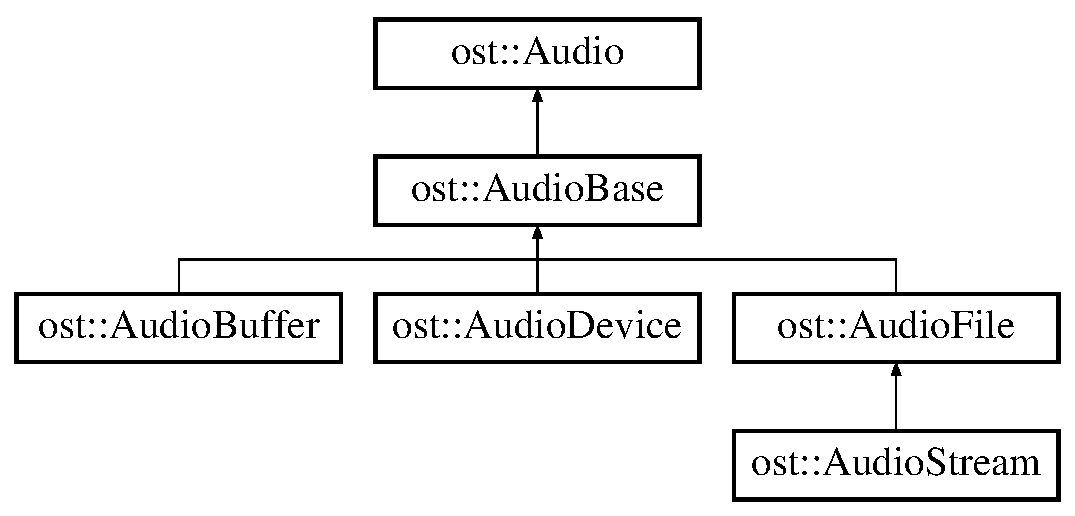
\includegraphics[height=4cm]{classost_1_1_audio_base}
\end{center}
\end{figure}
\subsection*{Public Member Functions}
\begin{DoxyCompactItemize}
\item 
{\bf AudioBase} ()
\begin{DoxyCompactList}\small\item\em Create audio base object with no info. \item\end{DoxyCompactList}\item 
{\bf AudioBase} (Info $\ast${\bf info})
\begin{DoxyCompactList}\small\item\em Create audio base object with audio source description. \item\end{DoxyCompactList}\item 
virtual {\bf $\sim$AudioBase} ()
\begin{DoxyCompactList}\small\item\em Destroy an audio base object. \item\end{DoxyCompactList}\item 
{\bf Encoding} {\bf getEncoding} (void)
\begin{DoxyCompactList}\small\item\em Generic get encoding. \item\end{DoxyCompactList}\item 
unsigned {\bf getSampleRate} (void)
\begin{DoxyCompactList}\small\item\em Generic sample rate. \item\end{DoxyCompactList}\item 
virtual ssize\_\-t {\bf putBuffer} ({\bf Encoded} data, size\_\-t size)=0
\begin{DoxyCompactList}\small\item\em Abstract interface to put raw data. \item\end{DoxyCompactList}\item 
ssize\_\-t {\bf putNative} ({\bf Encoded} data, size\_\-t size)
\begin{DoxyCompactList}\small\item\em Puts raw data and does native to refined endian swapping if needed based on encoding type and local machine endian. \item\end{DoxyCompactList}\item 
virtual ssize\_\-t {\bf getBuffer} ({\bf Encoded} data, size\_\-t size)=0
\begin{DoxyCompactList}\small\item\em Abstract interface to get raw data. \item\end{DoxyCompactList}\item 
ssize\_\-t {\bf getPacket} ({\bf Encoded} data)
\begin{DoxyCompactList}\small\item\em Get's a packet of audio data. \item\end{DoxyCompactList}\item 
ssize\_\-t {\bf getNative} ({\bf Encoded} data, size\_\-t size)
\begin{DoxyCompactList}\small\item\em Get raw data and assure is in native machine endian. \item\end{DoxyCompactList}\end{DoxyCompactItemize}
\subsection*{Protected Attributes}
\begin{DoxyCompactItemize}
\item 
Info {\bf info}
\end{DoxyCompactItemize}


\subsection{Detailed Description}
\doxyref{AudioBase}{p.}{classost_1_1_audio_base} base class for many other audio classes which stream data. common audio stream base. 

\subsection{Constructor \& Destructor Documentation}
\index{ost::AudioBase@{ost::AudioBase}!AudioBase@{AudioBase}}
\index{AudioBase@{AudioBase}!ost::AudioBase@{ost::AudioBase}}
\subsubsection[{AudioBase}]{\setlength{\rightskip}{0pt plus 5cm}ost::AudioBase::AudioBase ()}\label{classost_1_1_audio_base_a78b761e7276b8c6ea542130aa3a6fde6}


Create audio base object with no info. \index{ost::AudioBase@{ost::AudioBase}!AudioBase@{AudioBase}}
\index{AudioBase@{AudioBase}!ost::AudioBase@{ost::AudioBase}}
\subsubsection[{AudioBase}]{\setlength{\rightskip}{0pt plus 5cm}ost::AudioBase::AudioBase (Info $\ast$ {\em info})}\label{classost_1_1_audio_base_a4f33a17bc5d215b5a5c6dac3758971d7}


Create audio base object with audio source description. 
\begin{DoxyParams}{Parameters}
\item[{\em info}]source description. \end{DoxyParams}
\index{ost::AudioBase@{ost::AudioBase}!$\sim$AudioBase@{$\sim$AudioBase}}
\index{$\sim$AudioBase@{$\sim$AudioBase}!ost::AudioBase@{ost::AudioBase}}
\subsubsection[{$\sim$AudioBase}]{\setlength{\rightskip}{0pt plus 5cm}virtual ost::AudioBase::$\sim$AudioBase ()\hspace{0.3cm}{\ttfamily  [virtual]}}\label{classost_1_1_audio_base_a932477ed1dab1f1251a22b3c75f0e745}


Destroy an audio base object. 

\subsection{Member Function Documentation}
\index{ost::AudioBase@{ost::AudioBase}!getBuffer@{getBuffer}}
\index{getBuffer@{getBuffer}!ost::AudioBase@{ost::AudioBase}}
\subsubsection[{getBuffer}]{\setlength{\rightskip}{0pt plus 5cm}virtual ssize\_\-t ost::AudioBase::getBuffer ({\bf Encoded} {\em data}, \/  size\_\-t {\em size})\hspace{0.3cm}{\ttfamily  [pure virtual]}}\label{classost_1_1_audio_base_ac2efc5edeab71de84764796d4353a057}


Abstract interface to get raw data. \begin{DoxyReturn}{Returns}
data received in buffer. 
\end{DoxyReturn}

\begin{DoxyParams}{Parameters}
\item[{\em data}]to get. \item[{\em size}]of data to get. \end{DoxyParams}


Implemented in {\bf ost::AudioBuffer} \doxyref{}{p.}{classost_1_1_audio_buffer_afd4bc8c265125e0809165c50ee2dac57}, {\bf ost::AudioFile} \doxyref{}{p.}{classost_1_1_audio_file_a40e6fcddf43df289fef2f66ccbe84bbd}, {\bf ost::AudioStream} \doxyref{}{p.}{classost_1_1_audio_stream_a32945278bd2fcb2b03c97f15d78f571b}, and {\bf ost::AudioDevice} \doxyref{}{p.}{classost_1_1_audio_device_a93d1081a88acc1cb9da1ab2e98a8c791}.\index{ost::AudioBase@{ost::AudioBase}!getEncoding@{getEncoding}}
\index{getEncoding@{getEncoding}!ost::AudioBase@{ost::AudioBase}}
\subsubsection[{getEncoding}]{\setlength{\rightskip}{0pt plus 5cm}{\bf Encoding} ost::AudioBase::getEncoding (void)\hspace{0.3cm}{\ttfamily  [inline]}}\label{classost_1_1_audio_base_ac419b6c2407894a81147e05f5c5eed9c}


Generic get encoding. \begin{DoxyReturn}{Returns}
audio encoding of this object. 
\end{DoxyReturn}


Reimplemented in {\bf ost::AudioFile} \doxyref{}{p.}{classost_1_1_audio_file_a7b9b5e2d9b8358477874aed0c610ee38}.\index{ost::AudioBase@{ost::AudioBase}!getNative@{getNative}}
\index{getNative@{getNative}!ost::AudioBase@{ost::AudioBase}}
\subsubsection[{getNative}]{\setlength{\rightskip}{0pt plus 5cm}ssize\_\-t ost::AudioBase::getNative ({\bf Encoded} {\em data}, \/  size\_\-t {\em size})}\label{classost_1_1_audio_base_a8333d7f0135dad5eaf515895c08dbfbd}


Get raw data and assure is in native machine endian. \begin{DoxyReturn}{Returns}
data received in buffer. 
\end{DoxyReturn}

\begin{DoxyParams}{Parameters}
\item[{\em data}]to get. \item[{\em size}]of data to get. \end{DoxyParams}
\index{ost::AudioBase@{ost::AudioBase}!getPacket@{getPacket}}
\index{getPacket@{getPacket}!ost::AudioBase@{ost::AudioBase}}
\subsubsection[{getPacket}]{\setlength{\rightskip}{0pt plus 5cm}ssize\_\-t ost::AudioBase::getPacket ({\bf Encoded} {\em data})\hspace{0.3cm}{\ttfamily  [inline]}}\label{classost_1_1_audio_base_a26a26fef0bcc5a158dab9cdf5a0d772e}


Get's a packet of audio data. \begin{DoxyReturn}{Returns}
count of data received. 
\end{DoxyReturn}

\begin{DoxyParams}{Parameters}
\item[{\em data}]to get. \end{DoxyParams}


Reimplemented in {\bf ost::AudioStream} \doxyref{}{p.}{classost_1_1_audio_stream_aab3a8568a6e1b3c9660a6c63b049ccd6}.\index{ost::AudioBase@{ost::AudioBase}!getSampleRate@{getSampleRate}}
\index{getSampleRate@{getSampleRate}!ost::AudioBase@{ost::AudioBase}}
\subsubsection[{getSampleRate}]{\setlength{\rightskip}{0pt plus 5cm}unsigned ost::AudioBase::getSampleRate (void)\hspace{0.3cm}{\ttfamily  [inline]}}\label{classost_1_1_audio_base_a438fa2853fd7683b06a5939c115aaa4c}


Generic sample rate. \begin{DoxyReturn}{Returns}
audio sample rate of this object. 
\end{DoxyReturn}


Reimplemented in {\bf ost::AudioFile} \doxyref{}{p.}{classost_1_1_audio_file_a3d271f6b81b9e9840150490d4725c620}.\index{ost::AudioBase@{ost::AudioBase}!putBuffer@{putBuffer}}
\index{putBuffer@{putBuffer}!ost::AudioBase@{ost::AudioBase}}
\subsubsection[{putBuffer}]{\setlength{\rightskip}{0pt plus 5cm}virtual ssize\_\-t ost::AudioBase::putBuffer ({\bf Encoded} {\em data}, \/  size\_\-t {\em size})\hspace{0.3cm}{\ttfamily  [pure virtual]}}\label{classost_1_1_audio_base_a4f8127866aad2198934215ea55e892a2}


Abstract interface to put raw data. 
\begin{DoxyParams}{Parameters}
\item[{\em data}]to put. \item[{\em size}]of data to put. \end{DoxyParams}
\begin{DoxyReturn}{Returns}
number of bytes actually put. 
\end{DoxyReturn}


Implemented in {\bf ost::AudioBuffer} \doxyref{}{p.}{classost_1_1_audio_buffer_a398d028be8c691e8107073308f4507bc}, {\bf ost::AudioFile} \doxyref{}{p.}{classost_1_1_audio_file_a6d53c942621cae134b021b57064b4004}, and {\bf ost::AudioDevice} \doxyref{}{p.}{classost_1_1_audio_device_af385b8b82740059b92e115082247a613}.\index{ost::AudioBase@{ost::AudioBase}!putNative@{putNative}}
\index{putNative@{putNative}!ost::AudioBase@{ost::AudioBase}}
\subsubsection[{putNative}]{\setlength{\rightskip}{0pt plus 5cm}ssize\_\-t ost::AudioBase::putNative ({\bf Encoded} {\em data}, \/  size\_\-t {\em size})}\label{classost_1_1_audio_base_a4f515f81fd2079b74ab93eee4947d9fb}


Puts raw data and does native to refined endian swapping if needed based on encoding type and local machine endian. 
\begin{DoxyParams}{Parameters}
\item[{\em data}]to put. \item[{\em size}]of data to put. \end{DoxyParams}
\begin{DoxyReturn}{Returns}
number of bytes actually put. 
\end{DoxyReturn}


\subsection{Member Data Documentation}
\index{ost::AudioBase@{ost::AudioBase}!info@{info}}
\index{info@{info}!ost::AudioBase@{ost::AudioBase}}
\subsubsection[{info}]{\setlength{\rightskip}{0pt plus 5cm}Info {\bf ost::AudioBase::info}\hspace{0.3cm}{\ttfamily  [protected]}}\label{classost_1_1_audio_base_aaf541ba0c6e8285e961d551454aa63a1}


The documentation for this class was generated from the following file:\begin{DoxyCompactItemize}
\item 
{\bf audio2.h}\end{DoxyCompactItemize}

\section{ost::AudioBuffer Class Reference}
\label{classost_1_1_audio_buffer}\index{ost::AudioBuffer@{ost::AudioBuffer}}


The \doxyref{AudioBuffer}{p.}{classost_1_1_audio_buffer} class is for mixing one-\/to-\/one soft joins.  


{\ttfamily \#include $<$audio2.h$>$}Inheritance diagram for ost::AudioBuffer::\begin{figure}[H]
\begin{center}
\leavevmode
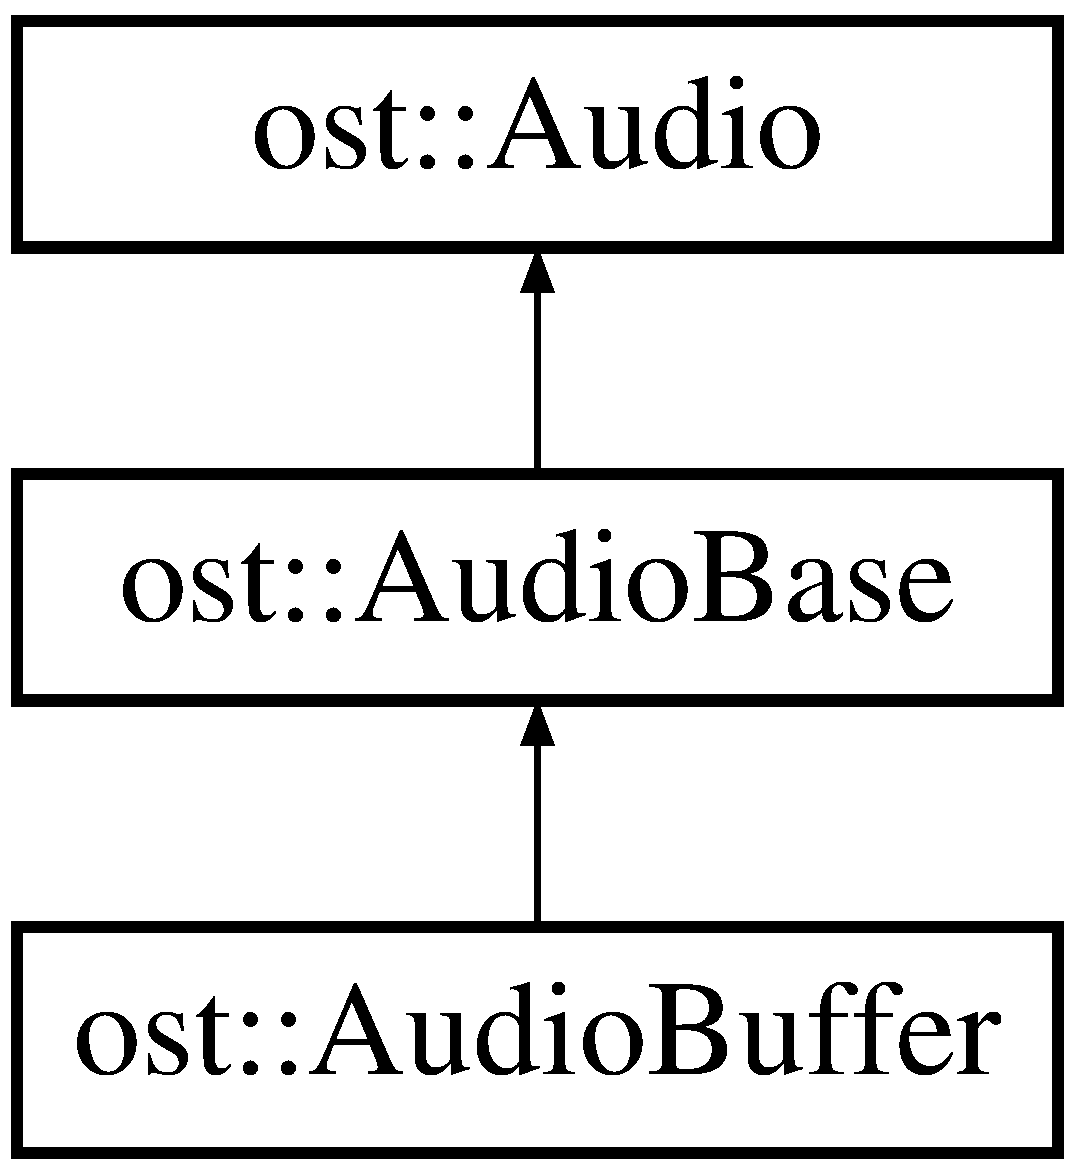
\includegraphics[height=3cm]{classost_1_1_audio_buffer}
\end{center}
\end{figure}
\subsection*{Public Member Functions}
\begin{DoxyCompactItemize}
\item 
{\bf AudioBuffer} ({\bf Info} $\ast${\bf info}, size\_\-t size=4096)
\item 
virtual {\bf $\sim$AudioBuffer} ()
\item 
ssize\_\-t {\bf getBuffer} ({\bf Encoded} data, size\_\-t number)
\begin{DoxyCompactList}\small\item\em save audio data from buffer data. \item\end{DoxyCompactList}\item 
ssize\_\-t {\bf putBuffer} ({\bf Encoded} data, size\_\-t number)
\begin{DoxyCompactList}\small\item\em Put data into the audio buffer. \item\end{DoxyCompactList}\end{DoxyCompactItemize}


\subsection{Detailed Description}
The \doxyref{AudioBuffer}{p.}{classost_1_1_audio_buffer} class is for mixing one-\/to-\/one soft joins. \begin{DoxyAuthor}{Author}
Mark Lipscombe $<${\tt markl@gasupnow.com}$>$ audio buffer mixer class 
\end{DoxyAuthor}


\subsection{Constructor \& Destructor Documentation}
\index{ost::AudioBuffer@{ost::AudioBuffer}!AudioBuffer@{AudioBuffer}}
\index{AudioBuffer@{AudioBuffer}!ost::AudioBuffer@{ost::AudioBuffer}}
\subsubsection[{AudioBuffer}]{\setlength{\rightskip}{0pt plus 5cm}ost::AudioBuffer::AudioBuffer ({\bf Info} $\ast$ {\em info}, \/  size\_\-t {\em size} = {\ttfamily 4096})}\label{classost_1_1_audio_buffer_a39ddb2920d6b421dabca98ac92221996}
\index{ost::AudioBuffer@{ost::AudioBuffer}!$\sim$AudioBuffer@{$\sim$AudioBuffer}}
\index{$\sim$AudioBuffer@{$\sim$AudioBuffer}!ost::AudioBuffer@{ost::AudioBuffer}}
\subsubsection[{$\sim$AudioBuffer}]{\setlength{\rightskip}{0pt plus 5cm}virtual ost::AudioBuffer::$\sim$AudioBuffer ()\hspace{0.3cm}{\ttfamily  [virtual]}}\label{classost_1_1_audio_buffer_a7829566cc5246824dcb670df9ae75233}


\subsection{Member Function Documentation}
\index{ost::AudioBuffer@{ost::AudioBuffer}!getBuffer@{getBuffer}}
\index{getBuffer@{getBuffer}!ost::AudioBuffer@{ost::AudioBuffer}}
\subsubsection[{getBuffer}]{\setlength{\rightskip}{0pt plus 5cm}ssize\_\-t ost::AudioBuffer::getBuffer ({\bf Encoded} {\em data}, \/  size\_\-t {\em number})\hspace{0.3cm}{\ttfamily  [virtual]}}\label{classost_1_1_audio_buffer_afd4bc8c265125e0809165c50ee2dac57}


save audio data from buffer data. \begin{DoxyReturn}{Returns}
number of bytes actually saved. 
\end{DoxyReturn}

\begin{DoxyParams}{Parameters}
\item[{\em data}]save buffer. \item[{\em number}]of bytes to save. \end{DoxyParams}


Implements {\bf ost::AudioBase} \doxyref{}{p.}{classost_1_1_audio_base_ac2efc5edeab71de84764796d4353a057}.\index{ost::AudioBuffer@{ost::AudioBuffer}!putBuffer@{putBuffer}}
\index{putBuffer@{putBuffer}!ost::AudioBuffer@{ost::AudioBuffer}}
\subsubsection[{putBuffer}]{\setlength{\rightskip}{0pt plus 5cm}ssize\_\-t ost::AudioBuffer::putBuffer ({\bf Encoded} {\em data}, \/  size\_\-t {\em number})\hspace{0.3cm}{\ttfamily  [virtual]}}\label{classost_1_1_audio_buffer_a398d028be8c691e8107073308f4507bc}


Put data into the audio buffer. \begin{DoxyReturn}{Returns}
number of bytes actually put. 
\end{DoxyReturn}

\begin{DoxyParams}{Parameters}
\item[{\em data}]of data to load. \item[{\em number}]of bytes to load. \end{DoxyParams}


Implements {\bf ost::AudioBase} \doxyref{}{p.}{classost_1_1_audio_base_a4f8127866aad2198934215ea55e892a2}.

The documentation for this class was generated from the following file:\begin{DoxyCompactItemize}
\item 
{\bf audio2.h}\end{DoxyCompactItemize}

\section{ost::AudioCodec Class Reference}
\label{classost_1_1_audio_codec}\index{ost::AudioCodec@{ost::AudioCodec}}


The codec class is a virtual used for transcoding audio samples between linear frames (or other known format) and an encoded \char`\"{}sample\char`\"{} buffer.  


{\ttfamily \#include $<$audio2.h$>$}Inheritance diagram for ost::AudioCodec::\begin{figure}[H]
\begin{center}
\leavevmode
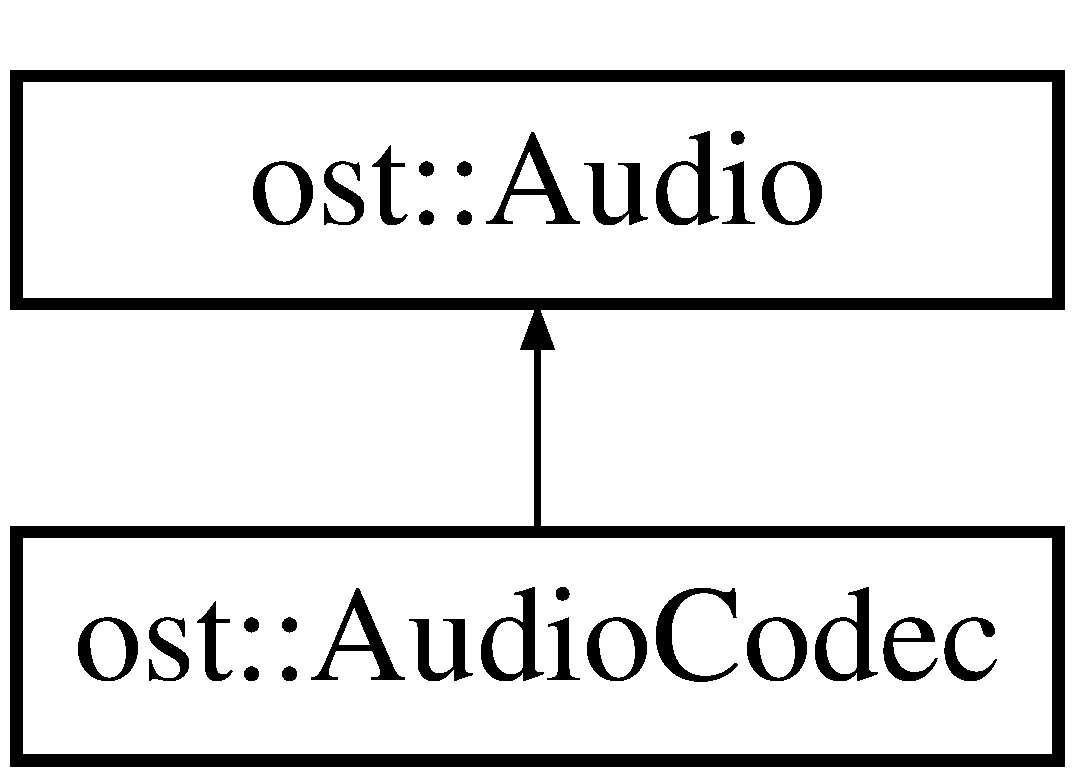
\includegraphics[height=2cm]{classost_1_1_audio_codec}
\end{center}
\end{figure}
\subsection*{Public Member Functions}
\begin{DoxyCompactItemize}
\item 
{\bf AudioCodec} (const char $\ast${\bf name}, {\bf Encoding} {\bf encoding})
\begin{DoxyCompactList}\small\item\em Base for codecs, create a named coded of a specific encoding. \item\end{DoxyCompactList}\item 
virtual {\bf $\sim$AudioCodec} ()
\item 
virtual {\bf Level} {\bf getImpulse} (void $\ast$buffer, unsigned number=0)
\begin{DoxyCompactList}\small\item\em Get the impulse energy level of a frame of X samples in the specified codec format. \item\end{DoxyCompactList}\item 
virtual {\bf Level} {\bf getPeak} (void $\ast$buffer, unsigned number=0)
\begin{DoxyCompactList}\small\item\em Get the peak energy level within the frame of X samples. \item\end{DoxyCompactList}\item 
virtual bool {\bf isSilent} ({\bf Level} threashold, void $\ast$buffer, unsigned number=0)
\begin{DoxyCompactList}\small\item\em Signal if the current audio frame is silent. \item\end{DoxyCompactList}\item 
virtual unsigned {\bf encode} ({\bf Linear} buffer, void $\ast$dest, unsigned number=0)=0
\begin{DoxyCompactList}\small\item\em Encode a linear sample frame into the codec sample buffer. \item\end{DoxyCompactList}\item 
virtual unsigned {\bf encodeBuffered} ({\bf Linear} Buffer, {\bf Encoded} dest, unsigned number)
\begin{DoxyCompactList}\small\item\em Encode linear samples buffered into the coded. \item\end{DoxyCompactList}\item 
virtual unsigned {\bf decode} ({\bf Linear} buffer, void $\ast$source, unsigned number=0)=0
\begin{DoxyCompactList}\small\item\em Decode the sample frame into linear samples. \item\end{DoxyCompactList}\item 
virtual unsigned {\bf decodeBuffered} ({\bf Linear} buffer, {\bf Encoded} source, unsigned len)
\begin{DoxyCompactList}\small\item\em Buffer and decode data into linear samples. \item\end{DoxyCompactList}\item 
virtual unsigned {\bf getEstimated} (void)
\begin{DoxyCompactList}\small\item\em Get estimated data required for buffered operations. \item\end{DoxyCompactList}\item 
virtual unsigned {\bf getRequired} (void)
\begin{DoxyCompactList}\small\item\em get required samples for encoding. \item\end{DoxyCompactList}\item 
virtual unsigned {\bf getPacket} ({\bf Encoded} destination, {\bf Encoded} data, unsigned size)
\begin{DoxyCompactList}\small\item\em Get a packet of data rather than decode. \item\end{DoxyCompactList}\item 
{\bf Info} {\bf getInfo} (void)
\begin{DoxyCompactList}\small\item\em Get an info description for this codec. \item\end{DoxyCompactList}\end{DoxyCompactItemize}
\subsection*{Static Public Member Functions}
\begin{DoxyCompactItemize}
\item 
static void {\bf endCodec} ({\bf AudioCodec} $\ast$codec)
\begin{DoxyCompactList}\small\item\em End use of a requested codec. \item\end{DoxyCompactList}\item 
static {\bf AudioCodec} $\ast$ {\bf getCodec} ({\bf Encoding} {\bf encoding}, const char $\ast$format=NULL, bool loaded=false)
\begin{DoxyCompactList}\small\item\em Get the codec base class for accessing a specific derived codec identified by encoding type and optional spd info. \item\end{DoxyCompactList}\item 
static {\bf AudioCodec} $\ast$ {\bf getCodec} ({\bf Info} \&{\bf info}, bool loaded=false)
\begin{DoxyCompactList}\small\item\em Get the codec base class for accessing a specific derived codec identified by audio source descriptor. \item\end{DoxyCompactList}\item 
static bool {\bf load} (const char $\ast${\bf name})
\begin{DoxyCompactList}\small\item\em Load a named codec set into process memory. \item\end{DoxyCompactList}\item 
static bool {\bf load} ({\bf Encoding} {\bf encoding})
\begin{DoxyCompactList}\small\item\em Find and load a codec file by it's encoding type. \item\end{DoxyCompactList}\end{DoxyCompactItemize}
\subsection*{Protected Member Functions}
\begin{DoxyCompactItemize}
\item 
{\bf AudioCodec} ()
\item 
virtual {\bf AudioCodec} $\ast$ {\bf getByFormat} (const char $\ast$format)
\begin{DoxyCompactList}\small\item\em often used to create a \char`\"{}new\char`\"{} codec of a subtype based on encoding format, default returns the current codec entity. \item\end{DoxyCompactList}\item 
virtual {\bf AudioCodec} $\ast$ {\bf getByInfo} ({\bf Info} \&{\bf info})
\begin{DoxyCompactList}\small\item\em get a codec by audio source info descriptor. \item\end{DoxyCompactList}\end{DoxyCompactItemize}
\subsection*{Protected Attributes}
\begin{DoxyCompactItemize}
\item 
{\bf AudioCodec} $\ast$ {\bf next}
\item 
{\bf Encoding} {\bf encoding}
\item 
const char $\ast$ {\bf name}
\item 
{\bf Info} {\bf info}
\end{DoxyCompactItemize}
\subsection*{Static Protected Attributes}
\begin{DoxyCompactItemize}
\item 
static {\bf AudioCodec} $\ast$ {\bf first}
\end{DoxyCompactItemize}


\subsection{Detailed Description}
The codec class is a virtual used for transcoding audio samples between linear frames (or other known format) and an encoded \char`\"{}sample\char`\"{} buffer. This class is only abstract and describes the core interface for loadable codec modules. This class is normally merged with AudioSample. A derived AudioCodecXXX will typically include a AudioRegisterXXX static class to automatically initialize and register the codec with the codec registry.

\begin{DoxyAuthor}{Author}
David Sugar $<${\tt dyfet@ostel.com}$>$ process codec interface. 
\end{DoxyAuthor}


\subsection{Constructor \& Destructor Documentation}
\index{ost::AudioCodec@{ost::AudioCodec}!AudioCodec@{AudioCodec}}
\index{AudioCodec@{AudioCodec}!ost::AudioCodec@{ost::AudioCodec}}
\subsubsection[{AudioCodec}]{\setlength{\rightskip}{0pt plus 5cm}ost::AudioCodec::AudioCodec ()\hspace{0.3cm}{\ttfamily  [protected]}}\label{classost_1_1_audio_codec_ac2d7cd36a4aff2eec71dad02ac7eb67f}
\index{ost::AudioCodec@{ost::AudioCodec}!AudioCodec@{AudioCodec}}
\index{AudioCodec@{AudioCodec}!ost::AudioCodec@{ost::AudioCodec}}
\subsubsection[{AudioCodec}]{\setlength{\rightskip}{0pt plus 5cm}ost::AudioCodec::AudioCodec (const char $\ast$ {\em name}, \/  {\bf Encoding} {\em encoding})}\label{classost_1_1_audio_codec_ad6b39c6b8e48636490586ca614d48d84}


Base for codecs, create a named coded of a specific encoding. 
\begin{DoxyParams}{Parameters}
\item[{\em name}]of codec. \item[{\em encoding}]type of codec. \end{DoxyParams}
\index{ost::AudioCodec@{ost::AudioCodec}!$\sim$AudioCodec@{$\sim$AudioCodec}}
\index{$\sim$AudioCodec@{$\sim$AudioCodec}!ost::AudioCodec@{ost::AudioCodec}}
\subsubsection[{$\sim$AudioCodec}]{\setlength{\rightskip}{0pt plus 5cm}virtual ost::AudioCodec::$\sim$AudioCodec ()\hspace{0.3cm}{\ttfamily  [inline, virtual]}}\label{classost_1_1_audio_codec_a4149a63324548a0cd1a4c268d41fd6e4}


\subsection{Member Function Documentation}
\index{ost::AudioCodec@{ost::AudioCodec}!decode@{decode}}
\index{decode@{decode}!ost::AudioCodec@{ost::AudioCodec}}
\subsubsection[{decode}]{\setlength{\rightskip}{0pt plus 5cm}virtual unsigned ost::AudioCodec::decode ({\bf Linear} {\em buffer}, \/  void $\ast$ {\em source}, \/  unsigned {\em number} = {\ttfamily 0})\hspace{0.3cm}{\ttfamily  [pure virtual]}}\label{classost_1_1_audio_codec_a907e86027d1511babd9446eca3b19850}


Decode the sample frame into linear samples. \begin{DoxyReturn}{Returns}
number of bytes scanned or returned 
\end{DoxyReturn}

\begin{DoxyParams}{Parameters}
\item[{\em buffer}]sample buffer to save linear samples into. \item[{\em source}]for encoded data. \item[{\em number}]of samples to extract. \end{DoxyParams}
\index{ost::AudioCodec@{ost::AudioCodec}!decodeBuffered@{decodeBuffered}}
\index{decodeBuffered@{decodeBuffered}!ost::AudioCodec@{ost::AudioCodec}}
\subsubsection[{decodeBuffered}]{\setlength{\rightskip}{0pt plus 5cm}virtual unsigned ost::AudioCodec::decodeBuffered ({\bf Linear} {\em buffer}, \/  {\bf Encoded} {\em source}, \/  unsigned {\em len})\hspace{0.3cm}{\ttfamily  [virtual]}}\label{classost_1_1_audio_codec_aa7f2d6b1965cdb86839ef55d9970e98e}


Buffer and decode data into linear samples. This is needed for audio formats that have irregular packet sizes.

\begin{DoxyReturn}{Returns}
number of samples actually decoded. 
\end{DoxyReturn}

\begin{DoxyParams}{Parameters}
\item[{\em destination}]for decoded data. \item[{\em source}]for encoded data. \item[{\em number}]of bytes being sent. \end{DoxyParams}
\index{ost::AudioCodec@{ost::AudioCodec}!encode@{encode}}
\index{encode@{encode}!ost::AudioCodec@{ost::AudioCodec}}
\subsubsection[{encode}]{\setlength{\rightskip}{0pt plus 5cm}virtual unsigned ost::AudioCodec::encode ({\bf Linear} {\em buffer}, \/  void $\ast$ {\em dest}, \/  unsigned {\em number} = {\ttfamily 0})\hspace{0.3cm}{\ttfamily  [pure virtual]}}\label{classost_1_1_audio_codec_ad9238d106a0a42bc63be63a305417fb8}


Encode a linear sample frame into the codec sample buffer. \begin{DoxyReturn}{Returns}
number of bytes written. 
\end{DoxyReturn}

\begin{DoxyParams}{Parameters}
\item[{\em buffer}]linear sample buffer to use. \item[{\em dest}]buffer to store encoded results. \item[{\em number}]of samples. \end{DoxyParams}
\index{ost::AudioCodec@{ost::AudioCodec}!encodeBuffered@{encodeBuffered}}
\index{encodeBuffered@{encodeBuffered}!ost::AudioCodec@{ost::AudioCodec}}
\subsubsection[{encodeBuffered}]{\setlength{\rightskip}{0pt plus 5cm}virtual unsigned ost::AudioCodec::encodeBuffered ({\bf Linear} {\em Buffer}, \/  {\bf Encoded} {\em dest}, \/  unsigned {\em number})\hspace{0.3cm}{\ttfamily  [virtual]}}\label{classost_1_1_audio_codec_ac430e489a59a79e0837500712e5bbed0}


Encode linear samples buffered into the coded. \begin{DoxyReturn}{Returns}
number of bytes written or 0 if incomplete. 
\end{DoxyReturn}

\begin{DoxyParams}{Parameters}
\item[{\em buffer}]linear samples to post. \item[{\em destination}]of encoded audio. \item[{\em number}]of samples being buffered. \end{DoxyParams}
\index{ost::AudioCodec@{ost::AudioCodec}!endCodec@{endCodec}}
\index{endCodec@{endCodec}!ost::AudioCodec@{ost::AudioCodec}}
\subsubsection[{endCodec}]{\setlength{\rightskip}{0pt plus 5cm}static void ost::AudioCodec::endCodec ({\bf AudioCodec} $\ast$ {\em codec})\hspace{0.3cm}{\ttfamily  [static]}}\label{classost_1_1_audio_codec_ad9c810876d4c61205d39e06a9b91e89a}


End use of a requested codec. If constructed then will be deleted.


\begin{DoxyParams}{Parameters}
\item[{\em codec}]pointer to getCodec returned coded pointer. \end{DoxyParams}
\index{ost::AudioCodec@{ost::AudioCodec}!getByFormat@{getByFormat}}
\index{getByFormat@{getByFormat}!ost::AudioCodec@{ost::AudioCodec}}
\subsubsection[{getByFormat}]{\setlength{\rightskip}{0pt plus 5cm}virtual {\bf AudioCodec}$\ast$ ost::AudioCodec::getByFormat (const char $\ast$ {\em format})\hspace{0.3cm}{\ttfamily  [inline, protected, virtual]}}\label{classost_1_1_audio_codec_ab82cde0fc2d640509eca21e4ef30ddee}


often used to create a \char`\"{}new\char`\"{} codec of a subtype based on encoding format, default returns the current codec entity. \begin{DoxyReturn}{Returns}
pointer to an active codec or NULL if not found. 
\end{DoxyReturn}

\begin{DoxyParams}{Parameters}
\item[{\em format}]name from spd. \end{DoxyParams}
\index{ost::AudioCodec@{ost::AudioCodec}!getByInfo@{getByInfo}}
\index{getByInfo@{getByInfo}!ost::AudioCodec@{ost::AudioCodec}}
\subsubsection[{getByInfo}]{\setlength{\rightskip}{0pt plus 5cm}virtual {\bf AudioCodec}$\ast$ ost::AudioCodec::getByInfo ({\bf Info} \& {\em info})\hspace{0.3cm}{\ttfamily  [inline, protected, virtual]}}\label{classost_1_1_audio_codec_ad68f933525fe820797b89aa1c91432af}


get a codec by audio source info descriptor. \begin{DoxyReturn}{Returns}
pointer to an active codec or NULL if not found. 
\end{DoxyReturn}

\begin{DoxyParams}{Parameters}
\item[{\em info}]audio source descriptor. \end{DoxyParams}
\index{ost::AudioCodec@{ost::AudioCodec}!getCodec@{getCodec}}
\index{getCodec@{getCodec}!ost::AudioCodec@{ost::AudioCodec}}
\subsubsection[{getCodec}]{\setlength{\rightskip}{0pt plus 5cm}static {\bf AudioCodec}$\ast$ ost::AudioCodec::getCodec ({\bf Info} \& {\em info}, \/  bool {\em loaded} = {\ttfamily false})\hspace{0.3cm}{\ttfamily  [static]}}\label{classost_1_1_audio_codec_adaf944bce5fd0ef5559ed660a8b405c3}


Get the codec base class for accessing a specific derived codec identified by audio source descriptor. \begin{DoxyReturn}{Returns}
pointer to codec for processing. 
\end{DoxyReturn}

\begin{DoxyParams}{Parameters}
\item[{\em info}]source descriptor for codec being requested. \item[{\em loaded}]true to load codec if not already in memory. \end{DoxyParams}
\index{ost::AudioCodec@{ost::AudioCodec}!getCodec@{getCodec}}
\index{getCodec@{getCodec}!ost::AudioCodec@{ost::AudioCodec}}
\subsubsection[{getCodec}]{\setlength{\rightskip}{0pt plus 5cm}static {\bf AudioCodec}$\ast$ ost::AudioCodec::getCodec ({\bf Encoding} {\em encoding}, \/  const char $\ast$ {\em format} = {\ttfamily NULL}, \/  bool {\em loaded} = {\ttfamily false})\hspace{0.3cm}{\ttfamily  [static]}}\label{classost_1_1_audio_codec_a63e5170162bb09eac8f6d91bb920295f}


Get the codec base class for accessing a specific derived codec identified by encoding type and optional spd info. \begin{DoxyReturn}{Returns}
pointer to codec for processing. 
\end{DoxyReturn}

\begin{DoxyParams}{Parameters}
\item[{\em encoding}]format requested. \item[{\em format}]spd options to pass to codec being created. \item[{\em loaded}]true to load if not already in memory. \end{DoxyParams}
\index{ost::AudioCodec@{ost::AudioCodec}!getEstimated@{getEstimated}}
\index{getEstimated@{getEstimated}!ost::AudioCodec@{ost::AudioCodec}}
\subsubsection[{getEstimated}]{\setlength{\rightskip}{0pt plus 5cm}virtual unsigned ost::AudioCodec::getEstimated (void)\hspace{0.3cm}{\ttfamily  [virtual]}}\label{classost_1_1_audio_codec_a0d02b2719ed4d628f2350aee72e789cc}


Get estimated data required for buffered operations. \begin{DoxyReturn}{Returns}
estimated number of bytes required for decode. 
\end{DoxyReturn}
\index{ost::AudioCodec@{ost::AudioCodec}!getImpulse@{getImpulse}}
\index{getImpulse@{getImpulse}!ost::AudioCodec@{ost::AudioCodec}}
\subsubsection[{getImpulse}]{\setlength{\rightskip}{0pt plus 5cm}virtual {\bf Level} ost::AudioCodec::getImpulse (void $\ast$ {\em buffer}, \/  unsigned {\em number} = {\ttfamily 0})\hspace{0.3cm}{\ttfamily  [virtual]}}\label{classost_1_1_audio_codec_a021a39d174853a4270f3f3775bfd634a}


Get the impulse energy level of a frame of X samples in the specified codec format. \begin{DoxyReturn}{Returns}
average impulse energy of frame (sumnation). 
\end{DoxyReturn}

\begin{DoxyParams}{Parameters}
\item[{\em buffer}]of encoded samples. \item[{\em number}]of encoded samples. \end{DoxyParams}
\index{ost::AudioCodec@{ost::AudioCodec}!getInfo@{getInfo}}
\index{getInfo@{getInfo}!ost::AudioCodec@{ost::AudioCodec}}
\subsubsection[{getInfo}]{\setlength{\rightskip}{0pt plus 5cm}{\bf Info} ost::AudioCodec::getInfo (void)\hspace{0.3cm}{\ttfamily  [inline]}}\label{classost_1_1_audio_codec_a564e2675bdab8ef4c957bde488c983e5}


Get an info description for this codec. \begin{DoxyReturn}{Returns}
info. 
\end{DoxyReturn}
\index{ost::AudioCodec@{ost::AudioCodec}!getPacket@{getPacket}}
\index{getPacket@{getPacket}!ost::AudioCodec@{ost::AudioCodec}}
\subsubsection[{getPacket}]{\setlength{\rightskip}{0pt plus 5cm}virtual unsigned ost::AudioCodec::getPacket ({\bf Encoded} {\em destination}, \/  {\bf Encoded} {\em data}, \/  unsigned {\em size})\hspace{0.3cm}{\ttfamily  [virtual]}}\label{classost_1_1_audio_codec_a760f86f0ace0420992bfa8bc1e8f68cf}


Get a packet of data rather than decode. This is tied with getEstimated.

\begin{DoxyReturn}{Returns}
size of data packet or 0 if not complete. 
\end{DoxyReturn}

\begin{DoxyParams}{Parameters}
\item[{\em destination}]to save. \item[{\em data}]to push into buffer. \item[{\em number}]of bytes to push. \end{DoxyParams}
\index{ost::AudioCodec@{ost::AudioCodec}!getPeak@{getPeak}}
\index{getPeak@{getPeak}!ost::AudioCodec@{ost::AudioCodec}}
\subsubsection[{getPeak}]{\setlength{\rightskip}{0pt plus 5cm}virtual {\bf Level} ost::AudioCodec::getPeak (void $\ast$ {\em buffer}, \/  unsigned {\em number} = {\ttfamily 0})\hspace{0.3cm}{\ttfamily  [virtual]}}\label{classost_1_1_audio_codec_a921946adef4203b24ba21ede710cfeb5}


Get the peak energy level within the frame of X samples. \begin{DoxyReturn}{Returns}
peak energy impulse in frame (largest). 
\end{DoxyReturn}

\begin{DoxyParams}{Parameters}
\item[{\em buffer}]of encoded samples. \item[{\em number}]of encoded samples. \end{DoxyParams}
\index{ost::AudioCodec@{ost::AudioCodec}!getRequired@{getRequired}}
\index{getRequired@{getRequired}!ost::AudioCodec@{ost::AudioCodec}}
\subsubsection[{getRequired}]{\setlength{\rightskip}{0pt plus 5cm}virtual unsigned ost::AudioCodec::getRequired (void)\hspace{0.3cm}{\ttfamily  [virtual]}}\label{classost_1_1_audio_codec_ab5164fbce2e6d1dde35554f039fb2379}


get required samples for encoding. \begin{DoxyReturn}{Returns}
required number of samples for encoder buffer. 
\end{DoxyReturn}
\index{ost::AudioCodec@{ost::AudioCodec}!isSilent@{isSilent}}
\index{isSilent@{isSilent}!ost::AudioCodec@{ost::AudioCodec}}
\subsubsection[{isSilent}]{\setlength{\rightskip}{0pt plus 5cm}virtual bool ost::AudioCodec::isSilent ({\bf Level} {\em threashold}, \/  void $\ast$ {\em buffer}, \/  unsigned {\em number} = {\ttfamily 0})\hspace{0.3cm}{\ttfamily  [virtual]}}\label{classost_1_1_audio_codec_aa444bf042a79428d91958a38973ded8e}


Signal if the current audio frame is silent. This can be deterimed either by an impulse computation, or, in some cases, some codecs may signal and flag silent packets.

\begin{DoxyReturn}{Returns}
true if silent 
\end{DoxyReturn}

\begin{DoxyParams}{Parameters}
\item[{\em threashold}]to use if not signaled. \item[{\em buffer}]of encoded samples. \item[{\em number}]of encoded samples. \end{DoxyParams}
\index{ost::AudioCodec@{ost::AudioCodec}!load@{load}}
\index{load@{load}!ost::AudioCodec@{ost::AudioCodec}}
\subsubsection[{load}]{\setlength{\rightskip}{0pt plus 5cm}static bool ost::AudioCodec::load ({\bf Encoding} {\em encoding})\hspace{0.3cm}{\ttfamily  [static]}}\label{classost_1_1_audio_codec_a15af308cffe36ef275772c9047b3b2b5}


Find and load a codec file by it's encoding type. Converts the type into a codec name and invokes the other loader...

\begin{DoxyReturn}{Returns}
true if successful. 
\end{DoxyReturn}

\begin{DoxyParams}{Parameters}
\item[{\em encoding}]type for file. \end{DoxyParams}
\index{ost::AudioCodec@{ost::AudioCodec}!load@{load}}
\index{load@{load}!ost::AudioCodec@{ost::AudioCodec}}
\subsubsection[{load}]{\setlength{\rightskip}{0pt plus 5cm}static bool ost::AudioCodec::load (const char $\ast$ {\em name})\hspace{0.3cm}{\ttfamily  [static]}}\label{classost_1_1_audio_codec_a7f2483c2267044701fdcca3549f4e8c8}


Load a named codec set into process memory. \begin{DoxyReturn}{Returns}
true if successful. 
\end{DoxyReturn}

\begin{DoxyParams}{Parameters}
\item[{\em name}]of codec set to load. \end{DoxyParams}


\subsection{Member Data Documentation}
\index{ost::AudioCodec@{ost::AudioCodec}!encoding@{encoding}}
\index{encoding@{encoding}!ost::AudioCodec@{ost::AudioCodec}}
\subsubsection[{encoding}]{\setlength{\rightskip}{0pt plus 5cm}{\bf Encoding} {\bf ost::AudioCodec::encoding}\hspace{0.3cm}{\ttfamily  [protected]}}\label{classost_1_1_audio_codec_a7c5e345679761e0b6c9958005af5e173}
\index{ost::AudioCodec@{ost::AudioCodec}!first@{first}}
\index{first@{first}!ost::AudioCodec@{ost::AudioCodec}}
\subsubsection[{first}]{\setlength{\rightskip}{0pt plus 5cm}{\bf AudioCodec}$\ast$ {\bf ost::AudioCodec::first}\hspace{0.3cm}{\ttfamily  [static, protected]}}\label{classost_1_1_audio_codec_a44ca187dbb88f91fc675f08aef30e523}
\index{ost::AudioCodec@{ost::AudioCodec}!info@{info}}
\index{info@{info}!ost::AudioCodec@{ost::AudioCodec}}
\subsubsection[{info}]{\setlength{\rightskip}{0pt plus 5cm}{\bf Info} {\bf ost::AudioCodec::info}\hspace{0.3cm}{\ttfamily  [protected]}}\label{classost_1_1_audio_codec_a4fb14af1f9c82f3b536f1c6ab8b53f69}
\index{ost::AudioCodec@{ost::AudioCodec}!name@{name}}
\index{name@{name}!ost::AudioCodec@{ost::AudioCodec}}
\subsubsection[{name}]{\setlength{\rightskip}{0pt plus 5cm}const char$\ast$ {\bf ost::AudioCodec::name}\hspace{0.3cm}{\ttfamily  [protected]}}\label{classost_1_1_audio_codec_a7eea163ba29813a936ccac616c83bb18}
\index{ost::AudioCodec@{ost::AudioCodec}!next@{next}}
\index{next@{next}!ost::AudioCodec@{ost::AudioCodec}}
\subsubsection[{next}]{\setlength{\rightskip}{0pt plus 5cm}{\bf AudioCodec}$\ast$ {\bf ost::AudioCodec::next}\hspace{0.3cm}{\ttfamily  [protected]}}\label{classost_1_1_audio_codec_acd455c04876aa5c5a42bd8fc9e43f620}


The documentation for this class was generated from the following file:\begin{DoxyCompactItemize}
\item 
{\bf audio2.h}\end{DoxyCompactItemize}

\section{ost::AudioDevice Class Reference}
\label{classost_1_1_audio_device}\index{ost::AudioDevice@{ost::AudioDevice}}


{\ttfamily \#include $<$audio2.h$>$}Inheritance diagram for ost::AudioDevice::\begin{figure}[H]
\begin{center}
\leavevmode
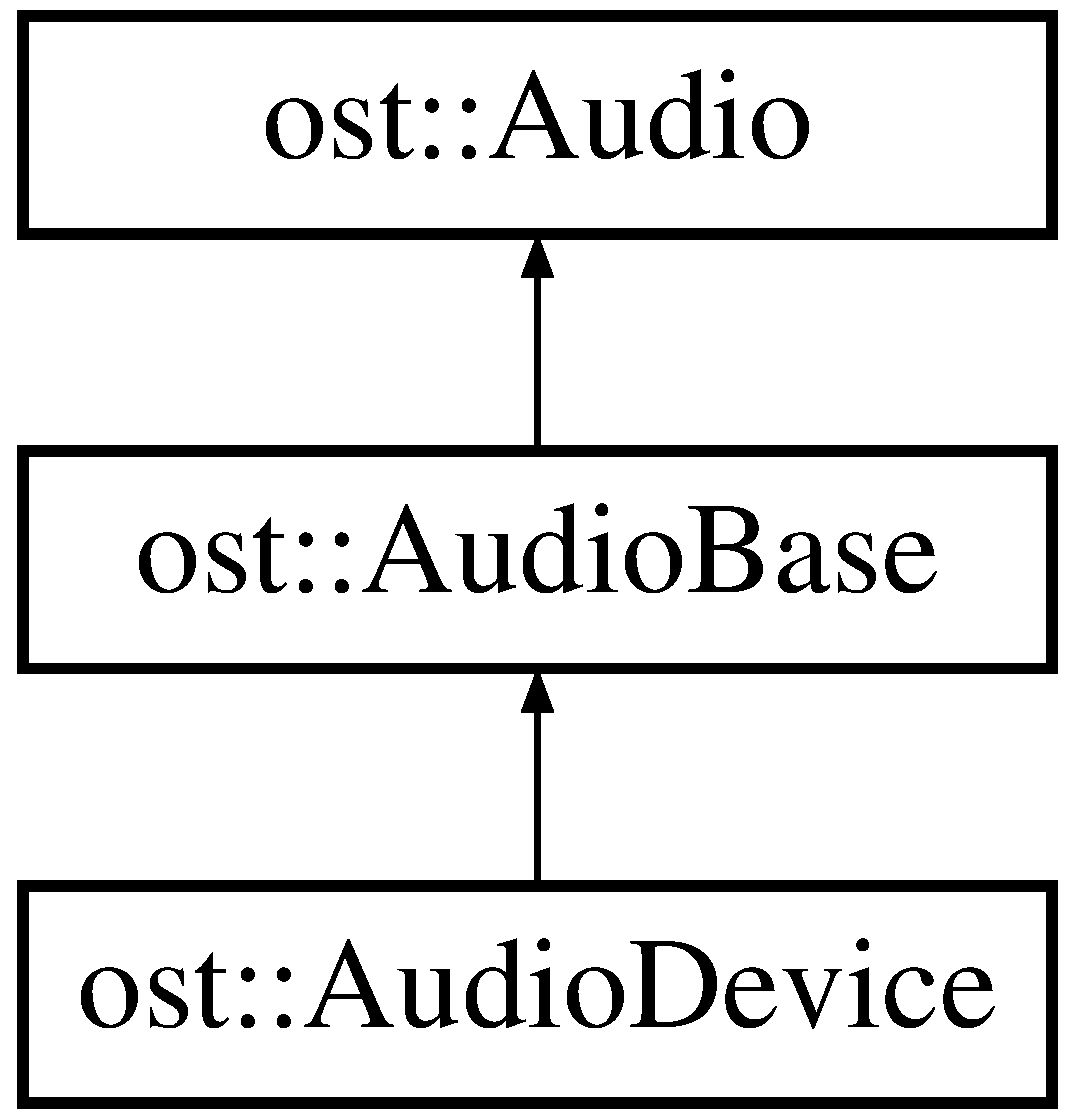
\includegraphics[height=3cm]{classost_1_1_audio_device}
\end{center}
\end{figure}
\subsection*{Public Member Functions}
\begin{DoxyCompactItemize}
\item 
virtual {\bf $\sim$AudioDevice} ()
\item 
virtual unsigned {\bf putSamples} ({\bf Linear} buffer, unsigned count)=0
\begin{DoxyCompactList}\small\item\em Copy linear samples to an audio device through its virtual. \item\end{DoxyCompactList}\item 
virtual unsigned {\bf getSamples} ({\bf Linear} buffer, unsigned count)=0
\begin{DoxyCompactList}\small\item\em Copy linear samples from an audio device through its virtual. \item\end{DoxyCompactList}\item 
virtual ssize\_\-t {\bf putBuffer} ({\bf Encoded} data, size\_\-t count)
\begin{DoxyCompactList}\small\item\em Copy audio encoded in the currently selected encoding for the audio device. \item\end{DoxyCompactList}\item 
virtual ssize\_\-t {\bf getBuffer} ({\bf Encoded} data, size\_\-t count)
\begin{DoxyCompactList}\small\item\em Record audio encoded in the currently selected encoding for the audio device. \item\end{DoxyCompactList}\item 
virtual bool {\bf setEncoded} ({\bf Info} \&{\bf info})
\begin{DoxyCompactList}\small\item\em Use encoding source descriptor to select the audio encoding format the audio device should be using. \item\end{DoxyCompactList}\item 
virtual bool {\bf setAudio} ({\bf Rate} rate=rate8khz, bool stereo=false, {\bf timeout\_\-t} framing=20)=0
\begin{DoxyCompactList}\small\item\em Set properties for audio device. \item\end{DoxyCompactList}\item 
virtual void {\bf sync} (void)
\begin{DoxyCompactList}\small\item\em Synchronize timing for audio device to next audio frame. \item\end{DoxyCompactList}\item 
virtual void {\bf flush} (void)=0
\begin{DoxyCompactList}\small\item\em Flush any pending buffered samples in audio device. \item\end{DoxyCompactList}\item 
unsigned {\bf bufMono} ({\bf Linear} buffer, unsigned count)
\begin{DoxyCompactList}\small\item\em Process linear mono audio and automatically convert to the encoding format the audio device is currently using. \item\end{DoxyCompactList}\item 
unsigned {\bf bufStereo} ({\bf Linear} buffer, unsigned count)
\begin{DoxyCompactList}\small\item\em Process linear stereo audio and automatically convert to the encoding format the audio device is currently using. \item\end{DoxyCompactList}\item 
{\bf Info} $\ast$ {\bf getInfo} (void)
\begin{DoxyCompactList}\small\item\em Get audio device source descriptor in effect for the device. \item\end{DoxyCompactList}\item 
bool {\bf isEnabled} (void)
\begin{DoxyCompactList}\small\item\em Whether device is currently enabled. \item\end{DoxyCompactList}\end{DoxyCompactItemize}
\subsection*{Protected Attributes}
\begin{DoxyCompactItemize}
\item 
bool {\bf enabled}
\end{DoxyCompactItemize}


\subsection{Constructor \& Destructor Documentation}
\index{ost::AudioDevice@{ost::AudioDevice}!$\sim$AudioDevice@{$\sim$AudioDevice}}
\index{$\sim$AudioDevice@{$\sim$AudioDevice}!ost::AudioDevice@{ost::AudioDevice}}
\subsubsection[{$\sim$AudioDevice}]{\setlength{\rightskip}{0pt plus 5cm}virtual ost::AudioDevice::$\sim$AudioDevice ()\hspace{0.3cm}{\ttfamily  [inline, virtual]}}\label{classost_1_1_audio_device_ae7c1477744fdb3821df5b09953bbe9ad}


\subsection{Member Function Documentation}
\index{ost::AudioDevice@{ost::AudioDevice}!bufMono@{bufMono}}
\index{bufMono@{bufMono}!ost::AudioDevice@{ost::AudioDevice}}
\subsubsection[{bufMono}]{\setlength{\rightskip}{0pt plus 5cm}unsigned ost::AudioDevice::bufMono ({\bf Linear} {\em buffer}, \/  unsigned {\em count})}\label{classost_1_1_audio_device_a385560f5f8d4781b387346d30c4ce345}


Process linear mono audio and automatically convert to the encoding format the audio device is currently using. If needed, automatically convert from mono to stereo.

\begin{DoxyReturn}{Returns}
number of samples played. 
\end{DoxyReturn}

\begin{DoxyParams}{Parameters}
\item[{\em buffer}]to linear mono audio data to play. \item[{\em count}]of linear mono audio samples to play. \end{DoxyParams}
\index{ost::AudioDevice@{ost::AudioDevice}!bufStereo@{bufStereo}}
\index{bufStereo@{bufStereo}!ost::AudioDevice@{ost::AudioDevice}}
\subsubsection[{bufStereo}]{\setlength{\rightskip}{0pt plus 5cm}unsigned ost::AudioDevice::bufStereo ({\bf Linear} {\em buffer}, \/  unsigned {\em count})}\label{classost_1_1_audio_device_ae6374d257f5c269a205eec7e1f596f6f}


Process linear stereo audio and automatically convert to the encoding format the audio device is currently using. If needed, automatically convert from stereo to mono.

\begin{DoxyReturn}{Returns}
number of samples played. 
\end{DoxyReturn}

\begin{DoxyParams}{Parameters}
\item[{\em buffer}]to linear stereo audio data to play. \item[{\em count}]of linear stereo audio samples to play. \end{DoxyParams}
\index{ost::AudioDevice@{ost::AudioDevice}!flush@{flush}}
\index{flush@{flush}!ost::AudioDevice@{ost::AudioDevice}}
\subsubsection[{flush}]{\setlength{\rightskip}{0pt plus 5cm}virtual void ost::AudioDevice::flush (void)\hspace{0.3cm}{\ttfamily  [pure virtual]}}\label{classost_1_1_audio_device_afaf42f23668d8eebc1fe367c7b33f9f4}


Flush any pending buffered samples in audio device. \index{ost::AudioDevice@{ost::AudioDevice}!getBuffer@{getBuffer}}
\index{getBuffer@{getBuffer}!ost::AudioDevice@{ost::AudioDevice}}
\subsubsection[{getBuffer}]{\setlength{\rightskip}{0pt plus 5cm}virtual ssize\_\-t ost::AudioDevice::getBuffer ({\bf Encoded} {\em data}, \/  size\_\-t {\em count})\hspace{0.3cm}{\ttfamily  [virtual]}}\label{classost_1_1_audio_device_a93d1081a88acc1cb9da1ab2e98a8c791}


Record audio encoded in the currently selected encoding for the audio device. 
\begin{DoxyParams}{Parameters}
\item[{\em data}]buffer for recording encoded audio. \item[{\em count}]of encoded bytes to record. \end{DoxyParams}
\begin{DoxyReturn}{Returns}
number of encoded bytes recorded. 
\end{DoxyReturn}


Implements {\bf ost::AudioBase} \doxyref{}{p.}{classost_1_1_audio_base_ac2efc5edeab71de84764796d4353a057}.\index{ost::AudioDevice@{ost::AudioDevice}!getInfo@{getInfo}}
\index{getInfo@{getInfo}!ost::AudioDevice@{ost::AudioDevice}}
\subsubsection[{getInfo}]{\setlength{\rightskip}{0pt plus 5cm}{\bf Info}$\ast$ ost::AudioDevice::getInfo (void)\hspace{0.3cm}{\ttfamily  [inline]}}\label{classost_1_1_audio_device_a6aecc79b2e3ac741af3cbba660ade7b9}


Get audio device source descriptor in effect for the device. \begin{DoxyReturn}{Returns}
audio device descriptor. 
\end{DoxyReturn}
\index{ost::AudioDevice@{ost::AudioDevice}!getSamples@{getSamples}}
\index{getSamples@{getSamples}!ost::AudioDevice@{ost::AudioDevice}}
\subsubsection[{getSamples}]{\setlength{\rightskip}{0pt plus 5cm}virtual unsigned ost::AudioDevice::getSamples ({\bf Linear} {\em buffer}, \/  unsigned {\em count})\hspace{0.3cm}{\ttfamily  [pure virtual]}}\label{classost_1_1_audio_device_a9797ed3fdf2fb6488f513e944f96dcfa}


Copy linear samples from an audio device through its virtual. 
\begin{DoxyParams}{Parameters}
\item[{\em buffer}]for recording. \item[{\em count}]of audio samples to record. \end{DoxyParams}
\begin{DoxyReturn}{Returns}
number of audio samples recorded. 
\end{DoxyReturn}
\index{ost::AudioDevice@{ost::AudioDevice}!isEnabled@{isEnabled}}
\index{isEnabled@{isEnabled}!ost::AudioDevice@{ost::AudioDevice}}
\subsubsection[{isEnabled}]{\setlength{\rightskip}{0pt plus 5cm}bool ost::AudioDevice::isEnabled (void)\hspace{0.3cm}{\ttfamily  [inline]}}\label{classost_1_1_audio_device_a2f991c8aef77c2fdf8690e08a192da64}


Whether device is currently enabled. If invalid audio settings are selected, it will be disabled until supported values are supplied.

\begin{DoxyReturn}{Returns}
enable state. 
\end{DoxyReturn}
\begin{DoxySeeAlso}{See also}
\doxyref{setAudio}{p.}{classost_1_1_audio_device_a80c44530fa49b79c8480b0543aadd425} setInfo 
\end{DoxySeeAlso}
\index{ost::AudioDevice@{ost::AudioDevice}!putBuffer@{putBuffer}}
\index{putBuffer@{putBuffer}!ost::AudioDevice@{ost::AudioDevice}}
\subsubsection[{putBuffer}]{\setlength{\rightskip}{0pt plus 5cm}virtual ssize\_\-t ost::AudioDevice::putBuffer ({\bf Encoded} {\em data}, \/  size\_\-t {\em count})\hspace{0.3cm}{\ttfamily  [virtual]}}\label{classost_1_1_audio_device_af385b8b82740059b92e115082247a613}


Copy audio encoded in the currently selected encoding for the audio device. 
\begin{DoxyParams}{Parameters}
\item[{\em data}]pointer to encoded data to play. \item[{\em count}]of encoded bytes to play. \end{DoxyParams}
\begin{DoxyReturn}{Returns}
number of encoded bytes played. 
\end{DoxyReturn}


Implements {\bf ost::AudioBase} \doxyref{}{p.}{classost_1_1_audio_base_a4f8127866aad2198934215ea55e892a2}.\index{ost::AudioDevice@{ost::AudioDevice}!putSamples@{putSamples}}
\index{putSamples@{putSamples}!ost::AudioDevice@{ost::AudioDevice}}
\subsubsection[{putSamples}]{\setlength{\rightskip}{0pt plus 5cm}virtual unsigned ost::AudioDevice::putSamples ({\bf Linear} {\em buffer}, \/  unsigned {\em count})\hspace{0.3cm}{\ttfamily  [pure virtual]}}\label{classost_1_1_audio_device_a71f1ac06b15596a907958d58724d200f}


Copy linear samples to an audio device through its virtual. 
\begin{DoxyParams}{Parameters}
\item[{\em buffer}]to linear audio data to play. \item[{\em count}]of audio samples to play. \end{DoxyParams}
\begin{DoxyReturn}{Returns}
number of audio samples played. 
\end{DoxyReturn}
\index{ost::AudioDevice@{ost::AudioDevice}!setAudio@{setAudio}}
\index{setAudio@{setAudio}!ost::AudioDevice@{ost::AudioDevice}}
\subsubsection[{setAudio}]{\setlength{\rightskip}{0pt plus 5cm}virtual bool ost::AudioDevice::setAudio ({\bf Rate} {\em rate} = {\ttfamily rate8khz}, \/  bool {\em stereo} = {\ttfamily false}, \/  {\bf timeout\_\-t} {\em framing} = {\ttfamily 20})\hspace{0.3cm}{\ttfamily  [pure virtual]}}\label{classost_1_1_audio_device_a80c44530fa49b79c8480b0543aadd425}


Set properties for audio device. 
\begin{DoxyParams}{Parameters}
\item[{\em rate}]of audio samples device should operate at. \item[{\em stereo}]flag. \item[{\em framing}]timer for default i/o framing for device. \end{DoxyParams}
\begin{DoxyReturn}{Returns}
false if settings not supported by device. 
\end{DoxyReturn}
\index{ost::AudioDevice@{ost::AudioDevice}!setEncoded@{setEncoded}}
\index{setEncoded@{setEncoded}!ost::AudioDevice@{ost::AudioDevice}}
\subsubsection[{setEncoded}]{\setlength{\rightskip}{0pt plus 5cm}virtual bool ost::AudioDevice::setEncoded ({\bf Info} \& {\em info})\hspace{0.3cm}{\ttfamily  [inline, virtual]}}\label{classost_1_1_audio_device_acf78ce4886758173a54ce91c0c1668d8}


Use encoding source descriptor to select the audio encoding format the audio device should be using. \begin{DoxyReturn}{Returns}
false if encoding format specified is unsupported by device 
\end{DoxyReturn}

\begin{DoxyParams}{Parameters}
\item[{\em info}]source description for device settings. \end{DoxyParams}
\index{ost::AudioDevice@{ost::AudioDevice}!sync@{sync}}
\index{sync@{sync}!ost::AudioDevice@{ost::AudioDevice}}
\subsubsection[{sync}]{\setlength{\rightskip}{0pt plus 5cm}virtual void ost::AudioDevice::sync (void)\hspace{0.3cm}{\ttfamily  [inline, virtual]}}\label{classost_1_1_audio_device_a61c2bceba12270f2f573a3bd01d1892e}


Synchronize timing for audio device to next audio frame. this is needed for audio devices which do not block i/o to assure one does not push too much data before the device can handle it. 

\subsection{Member Data Documentation}
\index{ost::AudioDevice@{ost::AudioDevice}!enabled@{enabled}}
\index{enabled@{enabled}!ost::AudioDevice@{ost::AudioDevice}}
\subsubsection[{enabled}]{\setlength{\rightskip}{0pt plus 5cm}bool {\bf ost::AudioDevice::enabled}\hspace{0.3cm}{\ttfamily  [protected]}}\label{classost_1_1_audio_device_ac99355626bd3b70a7b4551055279ad2b}


The documentation for this class was generated from the following file:\begin{DoxyCompactItemize}
\item 
{\bf audio2.h}\end{DoxyCompactItemize}

\section{ost::AudioFile Class Reference}
\label{classost_1_1_audio_file}\index{ost::AudioFile@{ost::AudioFile}}


A class used to manipulate audio data.  


{\ttfamily \#include $<$audio2.h$>$}Inheritance diagram for ost::AudioFile::\begin{figure}[H]
\begin{center}
\leavevmode
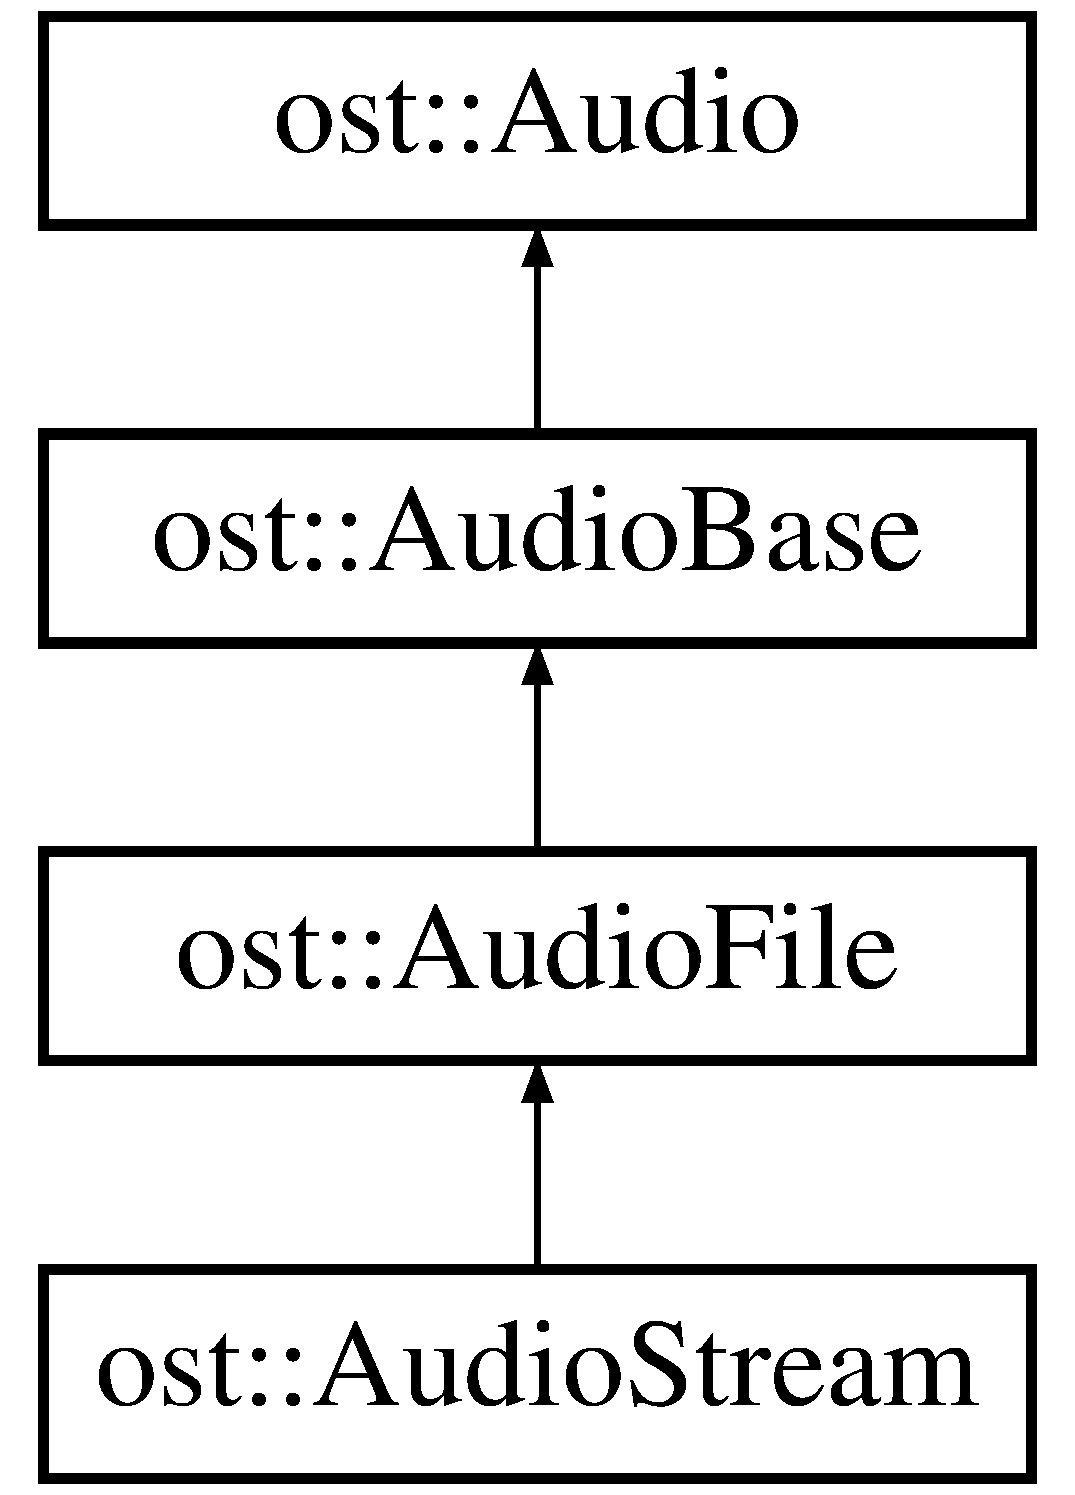
\includegraphics[height=4cm]{classost_1_1_audio_file}
\end{center}
\end{figure}
\subsection*{Public Member Functions}
\begin{DoxyCompactItemize}
\item 
{\bf AudioFile} (const char $\ast$name, unsigned long offset=0)
\begin{DoxyCompactList}\small\item\em Construct and open an existing audio file for read/write. \item\end{DoxyCompactList}\item 
{\bf AudioFile} (const char $\ast$name, {\bf Info} $\ast${\bf info}, unsigned long {\bf minimum}=0)
\begin{DoxyCompactList}\small\item\em Create and open a new audio file for writing. \item\end{DoxyCompactList}\item 
{\bf AudioFile} ()
\begin{DoxyCompactList}\small\item\em Construct an audio file without attaching to the filesystem. \item\end{DoxyCompactList}\item 
virtual {\bf $\sim$AudioFile} ()
\item 
void {\bf open} (const char $\ast$name, {\bf Mode} {\bf mode}=modeWrite, {\bf timeout\_\-t} framing=0)
\begin{DoxyCompactList}\small\item\em Open an audio file and associate it with this object. \item\end{DoxyCompactList}\item 
void {\bf create} (const char $\ast$name, {\bf Info} $\ast${\bf info}, bool exclusive=false, {\bf timeout\_\-t} framing=0)
\begin{DoxyCompactList}\small\item\em Create a new audio file and associate it with this object. \item\end{DoxyCompactList}\item 
time\_\-t {\bf getAge} (void)
\begin{DoxyCompactList}\small\item\em Returns age since last prior access. \item\end{DoxyCompactList}\item 
size\_\-t {\bf getSize} (void)
\begin{DoxyCompactList}\small\item\em Get maximum size of frame buffer for data use. \item\end{DoxyCompactList}\item 
void {\bf close} (void)
\begin{DoxyCompactList}\small\item\em Close an object associated with an open file. \item\end{DoxyCompactList}\item 
void {\bf clear} (void)
\begin{DoxyCompactList}\small\item\em Clear the \doxyref{AudioFile}{p.}{classost_1_1_audio_file} structure. \item\end{DoxyCompactList}\item 
ssize\_\-t {\bf getBuffer} ({\bf Encoded} buffer, size\_\-t len=0)
\begin{DoxyCompactList}\small\item\em Retrieve bytes from the file into a memory buffer. \item\end{DoxyCompactList}\item 
unsigned {\bf getLinear} ({\bf Linear} buffer, unsigned request=0)
\begin{DoxyCompactList}\small\item\em Retrieve and convert content to linear encoded audio data from it's original form. \item\end{DoxyCompactList}\item 
ssize\_\-t {\bf putBuffer} ({\bf Encoded} buffer, size\_\-t len=0)
\begin{DoxyCompactList}\small\item\em Insert bytes into the file from a memory buffer. \item\end{DoxyCompactList}\item 
unsigned {\bf putLinear} ({\bf Linear} buffer, unsigned request=0)
\begin{DoxyCompactList}\small\item\em Convert and store content from linear encoded audio data to the format of the audio file. \item\end{DoxyCompactList}\item 
{\bf Error} {\bf getSamples} (void $\ast$buffer, unsigned samples=0)
\begin{DoxyCompactList}\small\item\em Retrieve samples from the file into a memory buffer. \item\end{DoxyCompactList}\item 
{\bf Error} {\bf putSamples} (void $\ast$buffer, unsigned samples=0)
\begin{DoxyCompactList}\small\item\em Insert samples into the file from a memory buffer. \item\end{DoxyCompactList}\item 
{\bf Error} {\bf skip} (long number)
\begin{DoxyCompactList}\small\item\em Change the file position by skipping a specified number of audio samples of audio data. \item\end{DoxyCompactList}\item 
{\bf Error} {\bf setPosition} (unsigned long samples=$\sim$0l)
\begin{DoxyCompactList}\small\item\em Seek a file position by sample count. \item\end{DoxyCompactList}\item 
{\bf Error} {\bf position} (const char $\ast$timestamp)
\begin{DoxyCompactList}\small\item\em Seek a file position by timestamp. \item\end{DoxyCompactList}\item 
void {\bf getPosition} (char $\ast$timestamp, size\_\-t size)
\begin{DoxyCompactList}\small\item\em Return the timestamp of the current absolute file position. \item\end{DoxyCompactList}\item 
{\bf Error} {\bf setLimit} (unsigned long maximum=0l)
\begin{DoxyCompactList}\small\item\em Set the maximum file position for reading and writing of audio data by samples. \item\end{DoxyCompactList}\item 
{\bf Error} {\bf getInfo} ({\bf Info} $\ast${\bf info})
\begin{DoxyCompactList}\small\item\em Copy the source description of the audio file into the specified object. \item\end{DoxyCompactList}\item 
{\bf Error} {\bf setMinimum} (unsigned long {\bf minimum})
\begin{DoxyCompactList}\small\item\em Set minimum file size for a created file. \item\end{DoxyCompactList}\item 
unsigned long {\bf getAbsolutePosition} (void)
\begin{DoxyCompactList}\small\item\em Get the current file pointer in bytes relative to the start of the file. \item\end{DoxyCompactList}\item 
unsigned long {\bf getPosition} (void)
\begin{DoxyCompactList}\small\item\em Get the current file pointer in samples relative to the start of the sample buffer. \item\end{DoxyCompactList}\item 
virtual bool {\bf isOpen} (void)
\begin{DoxyCompactList}\small\item\em Test if the file is opened. \item\end{DoxyCompactList}\item 
virtual bool {\bf hasPositioning} (void)
\begin{DoxyCompactList}\small\item\em Return true if underlying derived class supports direct access to file positioning. \item\end{DoxyCompactList}\item 
{\bf Encoding} {\bf getEncoding} (void)
\begin{DoxyCompactList}\small\item\em Return audio encoding format for this audio file. \item\end{DoxyCompactList}\item 
{\bf Format} {\bf getFormat} (void)
\begin{DoxyCompactList}\small\item\em Return base file format of containing audio file. \item\end{DoxyCompactList}\item 
unsigned {\bf getSampleRate} (void)
\begin{DoxyCompactList}\small\item\em Get audio encoding sample rate, in samples per second, for this audio file. \item\end{DoxyCompactList}\item 
char $\ast$ {\bf getAnnotation} (void)
\begin{DoxyCompactList}\small\item\em Get annotation extracted from header of containing file. \item\end{DoxyCompactList}\item 
{\bf Error} {\bf getError} (void)
\begin{DoxyCompactList}\small\item\em Get last error code. \item\end{DoxyCompactList}\item 
bool {\bf operator!} (void)
\item 
bool {\bf isSigned} (void)
\begin{DoxyCompactList}\small\item\em Return if the current content is signed or unsigned samples. \item\end{DoxyCompactList}\end{DoxyCompactItemize}
\subsection*{Protected Member Functions}
\begin{DoxyCompactItemize}
\item 
void {\bf initialize} (void)
\item 
void {\bf getWaveFormat} (int size)
\item 
void {\bf mp3info} ({\bf mpeg\_\-audio} $\ast$mp3)
\item 
virtual bool {\bf afCreate} (const char $\ast$path, bool exclusive=false)
\item 
virtual bool {\bf afOpen} (const char $\ast$path, {\bf Mode} m=modeWrite)
\item 
virtual bool {\bf afPeek} (unsigned char $\ast$data, unsigned size)
\item 
{\bf AudioCodec} $\ast$ {\bf getCodec} (void)
\item 
virtual int {\bf afRead} (unsigned char $\ast$data, unsigned size)
\begin{DoxyCompactList}\small\item\em Read a given number of bytes from the file, starting from the current file pointer. \item\end{DoxyCompactList}\item 
virtual int {\bf afWrite} (unsigned char $\ast$data, unsigned size)
\begin{DoxyCompactList}\small\item\em Write a number of bytes into the file at the current file pointer. \item\end{DoxyCompactList}\item 
virtual bool {\bf afSeek} (unsigned long pos)
\begin{DoxyCompactList}\small\item\em Seek to the given position relative to the start of the file and set the file pointer. \item\end{DoxyCompactList}\item 
virtual void {\bf afClose} (void)
\begin{DoxyCompactList}\small\item\em Close the derived file handling system's file handle. \item\end{DoxyCompactList}\item 
virtual char $\ast$ {\bf getContinuation} (void)
\begin{DoxyCompactList}\small\item\em This function is used to splice multiple audio files together into a single stream of continues audio data. \item\end{DoxyCompactList}\item 
const char $\ast$ {\bf getErrorStr} ({\bf Error} err)
\begin{DoxyCompactList}\small\item\em Return a human-\/readable error message given a numeric error code of type \doxyref{Audio::Error}{p.}{classost_1_1_audio_a9b399c8c40f1c9c460490efeb3f86884}. \item\end{DoxyCompactList}\item 
{\bf Error} {\bf setError} ({\bf Error} err)
\item 
unsigned long {\bf getHeader} (void)
\begin{DoxyCompactList}\small\item\em Get number of bytes in the file header. \item\end{DoxyCompactList}\item 
unsigned short {\bf getShort} (unsigned char $\ast$data)
\begin{DoxyCompactList}\small\item\em Convert binary 2 byte data stored in the order specified in the source description into a short variable. \item\end{DoxyCompactList}\item 
void {\bf setShort} (unsigned char $\ast$data, unsigned short value)
\begin{DoxyCompactList}\small\item\em Save a short as two byte binary data stored in the endian order specified in the source description. \item\end{DoxyCompactList}\item 
unsigned long {\bf getLong} (unsigned char $\ast$data)
\begin{DoxyCompactList}\small\item\em Convert binary 4 byte data stored in the order specified in the source description into a long variable. \item\end{DoxyCompactList}\item 
void {\bf setLong} (unsigned char $\ast$data, unsigned long value)
\begin{DoxyCompactList}\small\item\em Save a long as four byte binary data stored in the endian order specified in the source description. \item\end{DoxyCompactList}\end{DoxyCompactItemize}
\subsection*{Protected Attributes}
\begin{DoxyCompactItemize}
\item 
char $\ast$ {\bf pathname}
\item 
{\bf Error} {\bf error}
\item 
unsigned long {\bf header}
\item 
unsigned long {\bf minimum}
\item 
unsigned long {\bf length}
\item 
\begin{tabbing}
xx\=xx\=xx\=xx\=xx\=xx\=xx\=xx\=xx\=\kill
union \{\\
\>int {\bf fd}\\
\>void $\ast$ {\bf handle}\\
\} {\bf file}\\

\end{tabbing}\item 
{\bf Mode} {\bf mode}
\item 
unsigned long {\bf iolimit}
\end{DoxyCompactItemize}


\subsection{Detailed Description}
A class used to manipulate audio data. This class provides file level access to audio data stored in different formats. This class also provides the ability to write audio data into a disk file.

\begin{DoxyAuthor}{Author}
David Sugar $<${\tt dyfet@ostel.com}$>$ audio file access. 
\end{DoxyAuthor}


\subsection{Constructor \& Destructor Documentation}
\index{ost::AudioFile@{ost::AudioFile}!AudioFile@{AudioFile}}
\index{AudioFile@{AudioFile}!ost::AudioFile@{ost::AudioFile}}
\subsubsection[{AudioFile}]{\setlength{\rightskip}{0pt plus 5cm}ost::AudioFile::AudioFile (const char $\ast$ {\em name}, \/  unsigned long {\em offset} = {\ttfamily 0})}\label{classost_1_1_audio_file_ab01d1c7365320d331e854552ecc953a2}


Construct and open an existing audio file for read/write. 
\begin{DoxyParams}{Parameters}
\item[{\em name}]of file to open. \item[{\em offset}]to start access. \end{DoxyParams}
\index{ost::AudioFile@{ost::AudioFile}!AudioFile@{AudioFile}}
\index{AudioFile@{AudioFile}!ost::AudioFile@{ost::AudioFile}}
\subsubsection[{AudioFile}]{\setlength{\rightskip}{0pt plus 5cm}ost::AudioFile::AudioFile (const char $\ast$ {\em name}, \/  {\bf Info} $\ast$ {\em info}, \/  unsigned long {\em minimum} = {\ttfamily 0})}\label{classost_1_1_audio_file_a112301bbb2b12e6a29e25437b1730aec}


Create and open a new audio file for writing. 
\begin{DoxyParams}{Parameters}
\item[{\em name}]of file to create. \item[{\em info}]source description for new file. \item[{\em minimum}]file size to accept at close. \end{DoxyParams}
\index{ost::AudioFile@{ost::AudioFile}!AudioFile@{AudioFile}}
\index{AudioFile@{AudioFile}!ost::AudioFile@{ost::AudioFile}}
\subsubsection[{AudioFile}]{\setlength{\rightskip}{0pt plus 5cm}ost::AudioFile::AudioFile ()\hspace{0.3cm}{\ttfamily  [inline]}}\label{classost_1_1_audio_file_a83e800eddbffcdf45dc4b196a87bd584}


Construct an audio file without attaching to the filesystem. \index{ost::AudioFile@{ost::AudioFile}!$\sim$AudioFile@{$\sim$AudioFile}}
\index{$\sim$AudioFile@{$\sim$AudioFile}!ost::AudioFile@{ost::AudioFile}}
\subsubsection[{$\sim$AudioFile}]{\setlength{\rightskip}{0pt plus 5cm}virtual ost::AudioFile::$\sim$AudioFile ()\hspace{0.3cm}{\ttfamily  [virtual]}}\label{classost_1_1_audio_file_acf8468ccbd7289cce50291e6f6ec0d53}


\subsection{Member Function Documentation}
\index{ost::AudioFile@{ost::AudioFile}!afClose@{afClose}}
\index{afClose@{afClose}!ost::AudioFile@{ost::AudioFile}}
\subsubsection[{afClose}]{\setlength{\rightskip}{0pt plus 5cm}virtual void ost::AudioFile::afClose (void)\hspace{0.3cm}{\ttfamily  [protected, virtual]}}\label{classost_1_1_audio_file_a22b33b82f3be60a5634617bf712bd39e}


Close the derived file handling system's file handle. \index{ost::AudioFile@{ost::AudioFile}!afCreate@{afCreate}}
\index{afCreate@{afCreate}!ost::AudioFile@{ost::AudioFile}}
\subsubsection[{afCreate}]{\setlength{\rightskip}{0pt plus 5cm}virtual bool ost::AudioFile::afCreate (const char $\ast$ {\em path}, \/  bool {\em exclusive} = {\ttfamily false})\hspace{0.3cm}{\ttfamily  [protected, virtual]}}\label{classost_1_1_audio_file_a4a271372f5c71ed212a38bcbd6bc78f1}
\index{ost::AudioFile@{ost::AudioFile}!afOpen@{afOpen}}
\index{afOpen@{afOpen}!ost::AudioFile@{ost::AudioFile}}
\subsubsection[{afOpen}]{\setlength{\rightskip}{0pt plus 5cm}virtual bool ost::AudioFile::afOpen (const char $\ast$ {\em path}, \/  {\bf Mode} {\em m} = {\ttfamily modeWrite})\hspace{0.3cm}{\ttfamily  [protected, virtual]}}\label{classost_1_1_audio_file_aac2bc808f80921302fab043b76e7fd1b}
\index{ost::AudioFile@{ost::AudioFile}!afPeek@{afPeek}}
\index{afPeek@{afPeek}!ost::AudioFile@{ost::AudioFile}}
\subsubsection[{afPeek}]{\setlength{\rightskip}{0pt plus 5cm}virtual bool ost::AudioFile::afPeek (unsigned char $\ast$ {\em data}, \/  unsigned {\em size})\hspace{0.3cm}{\ttfamily  [protected, virtual]}}\label{classost_1_1_audio_file_a8e849ce99910b88c7ce7d6def2b09713}
\index{ost::AudioFile@{ost::AudioFile}!afRead@{afRead}}
\index{afRead@{afRead}!ost::AudioFile@{ost::AudioFile}}
\subsubsection[{afRead}]{\setlength{\rightskip}{0pt plus 5cm}virtual int ost::AudioFile::afRead (unsigned char $\ast$ {\em data}, \/  unsigned {\em size})\hspace{0.3cm}{\ttfamily  [protected, virtual]}}\label{classost_1_1_audio_file_ad9ce6bffdc596b4131a0d2de1b9d3687}


Read a given number of bytes from the file, starting from the current file pointer. May be overridden by derived classes.


\begin{DoxyParams}{Parameters}
\item[{\em data}]A pointer to the buffer to copy the bytes to. \item[{\em size}]The number of bytes to read. \end{DoxyParams}
\begin{DoxyReturn}{Returns}
The number of bytes read, or -\/1 if an error occurs. On UNIX platforms, use strerror(errno) to get the human-\/readable error string or FormatMessage(GetLastError()) on Windows platforms. 
\end{DoxyReturn}
\index{ost::AudioFile@{ost::AudioFile}!afSeek@{afSeek}}
\index{afSeek@{afSeek}!ost::AudioFile@{ost::AudioFile}}
\subsubsection[{afSeek}]{\setlength{\rightskip}{0pt plus 5cm}virtual bool ost::AudioFile::afSeek (unsigned long {\em pos})\hspace{0.3cm}{\ttfamily  [protected, virtual]}}\label{classost_1_1_audio_file_abb103103800873c272940685d7d73bda}


Seek to the given position relative to the start of the file and set the file pointer. This does not use 64-\/bit clean seek functions, so seeking to positions greater than (2$^\wedge$32)-\/1 will result in undefined behavior.


\begin{DoxyParams}{Parameters}
\item[{\em pos}]The position to seek to. \end{DoxyParams}
\begin{DoxyReturn}{Returns}
true if successful, false otherwise. 
\end{DoxyReturn}
\index{ost::AudioFile@{ost::AudioFile}!afWrite@{afWrite}}
\index{afWrite@{afWrite}!ost::AudioFile@{ost::AudioFile}}
\subsubsection[{afWrite}]{\setlength{\rightskip}{0pt plus 5cm}virtual int ost::AudioFile::afWrite (unsigned char $\ast$ {\em data}, \/  unsigned {\em size})\hspace{0.3cm}{\ttfamily  [protected, virtual]}}\label{classost_1_1_audio_file_a79a6020d043bf65659a114420af86c04}


Write a number of bytes into the file at the current file pointer. May be overridden by derived classes.


\begin{DoxyParams}{Parameters}
\item[{\em data}]A pointer to the buffer with the bytes to write. \item[{\em size}]The number of bytes to write from the buffer. \end{DoxyParams}
\begin{DoxyReturn}{Returns}
The number of bytes written, or -\/1 if an error occurs. On UNIX platforms, use strerror(errno) to get the human-\/readable error string or FormatMessage(GetLastError()) on Windows platforms. 
\end{DoxyReturn}
\index{ost::AudioFile@{ost::AudioFile}!clear@{clear}}
\index{clear@{clear}!ost::AudioFile@{ost::AudioFile}}
\subsubsection[{clear}]{\setlength{\rightskip}{0pt plus 5cm}void ost::AudioFile::clear (void)}\label{classost_1_1_audio_file_a9ba09de7cf15f819a798fd10fed10060}


Clear the \doxyref{AudioFile}{p.}{classost_1_1_audio_file} structure. Called by \doxyref{AudioFile::close()}{p.}{classost_1_1_audio_file_aba0e5a66e006c61aef1ddbd018e2e7ed}. Sets all fields to zero and deletes the dynamically allocated memory pointed to by the pathname and info.annotation members. See \doxyref{AudioFile::initialize()}{p.}{classost_1_1_audio_file_a4bf7f795b71403f7f9946c105b5b5c5d} for the dynamic allocation code. \index{ost::AudioFile@{ost::AudioFile}!close@{close}}
\index{close@{close}!ost::AudioFile@{ost::AudioFile}}
\subsubsection[{close}]{\setlength{\rightskip}{0pt plus 5cm}void ost::AudioFile::close (void)}\label{classost_1_1_audio_file_aba0e5a66e006c61aef1ddbd018e2e7ed}


Close an object associated with an open file. This updates the header metadata with the file length if the file length has changed. 

Reimplemented in {\bf ost::AudioStream} \doxyref{}{p.}{classost_1_1_audio_stream_a823bf9a3d64dbae7117b6c29681017d3}.\index{ost::AudioFile@{ost::AudioFile}!create@{create}}
\index{create@{create}!ost::AudioFile@{ost::AudioFile}}
\subsubsection[{create}]{\setlength{\rightskip}{0pt plus 5cm}void ost::AudioFile::create (const char $\ast$ {\em name}, \/  {\bf Info} $\ast$ {\em info}, \/  bool {\em exclusive} = {\ttfamily false}, \/  {\bf timeout\_\-t} {\em framing} = {\ttfamily 0})}\label{classost_1_1_audio_file_af536da5d45926c3f75075c76f12ecb51}


Create a new audio file and associate it with this object. Called implicitly by the three-\/argument version of the constructor.


\begin{DoxyParams}{Parameters}
\item[{\em name}]The name of the file to open. \item[{\em info}]The type of the audio file to be created. \item[{\em exclusive}]create option. \item[{\em framing}]time in milliseconds. \end{DoxyParams}


Reimplemented in {\bf ost::AudioStream} \doxyref{}{p.}{classost_1_1_audio_stream_a58fd6f03aff924fdd330919caf543623}.\index{ost::AudioFile@{ost::AudioFile}!getAbsolutePosition@{getAbsolutePosition}}
\index{getAbsolutePosition@{getAbsolutePosition}!ost::AudioFile@{ost::AudioFile}}
\subsubsection[{getAbsolutePosition}]{\setlength{\rightskip}{0pt plus 5cm}unsigned long ost::AudioFile::getAbsolutePosition (void)}\label{classost_1_1_audio_file_a50401a6a8ab481d4e9a80cc4788c8d6d}


Get the current file pointer in bytes relative to the start of the file. See \doxyref{getPosition()}{p.}{classost_1_1_audio_file_affbf0d290dceff5b9974fd7b4f07eadc} to determine the position relative to the start of the sample buffer.

\begin{DoxyReturn}{Returns}
The current file pointer in bytes relative to the start of the file. Returns 0 if the file is not open, is empty, or an error has occured. 
\end{DoxyReturn}
\index{ost::AudioFile@{ost::AudioFile}!getAge@{getAge}}
\index{getAge@{getAge}!ost::AudioFile@{ost::AudioFile}}
\subsubsection[{getAge}]{\setlength{\rightskip}{0pt plus 5cm}time\_\-t ost::AudioFile::getAge (void)}\label{classost_1_1_audio_file_a5239719e8411bf6ee7f71a9f42ec9643}


Returns age since last prior access. Used for cache computations.

\begin{DoxyReturn}{Returns}
age in seconds. 
\end{DoxyReturn}
\index{ost::AudioFile@{ost::AudioFile}!getAnnotation@{getAnnotation}}
\index{getAnnotation@{getAnnotation}!ost::AudioFile@{ost::AudioFile}}
\subsubsection[{getAnnotation}]{\setlength{\rightskip}{0pt plus 5cm}char$\ast$ ost::AudioFile::getAnnotation (void)\hspace{0.3cm}{\ttfamily  [inline]}}\label{classost_1_1_audio_file_ae5c1671337f9c9c00e677065aaed6b38}


Get annotation extracted from header of containing file. \begin{DoxyReturn}{Returns}
annotation text if any, else NULL. 
\end{DoxyReturn}
\index{ost::AudioFile@{ost::AudioFile}!getBuffer@{getBuffer}}
\index{getBuffer@{getBuffer}!ost::AudioFile@{ost::AudioFile}}
\subsubsection[{getBuffer}]{\setlength{\rightskip}{0pt plus 5cm}ssize\_\-t ost::AudioFile::getBuffer ({\bf Encoded} {\em buffer}, \/  size\_\-t {\em len} = {\ttfamily 0})\hspace{0.3cm}{\ttfamily  [virtual]}}\label{classost_1_1_audio_file_a40e6fcddf43df289fef2f66ccbe84bbd}


Retrieve bytes from the file into a memory buffer. This increments the file pointer so subsequent calls read further bytes. If you want to read a number of samples rather than bytes, use \doxyref{getSamples()}{p.}{classost_1_1_audio_file_a9bb99aa5d59ef9414b8bac9b8086edad}.


\begin{DoxyParams}{Parameters}
\item[{\em buffer}]area to copy the samples to. \item[{\em len}]The number of bytes (not samples) to copy or 0 for frame. \end{DoxyParams}
\begin{DoxyReturn}{Returns}
The number of bytes (not samples) read. Returns -\/1 if no bytes are read and an error occurs. 
\end{DoxyReturn}


Implements {\bf ost::AudioBase} \doxyref{}{p.}{classost_1_1_audio_base_ac2efc5edeab71de84764796d4353a057}.

Reimplemented in {\bf ost::AudioStream} \doxyref{}{p.}{classost_1_1_audio_stream_a32945278bd2fcb2b03c97f15d78f571b}.\index{ost::AudioFile@{ost::AudioFile}!getCodec@{getCodec}}
\index{getCodec@{getCodec}!ost::AudioFile@{ost::AudioFile}}
\subsubsection[{getCodec}]{\setlength{\rightskip}{0pt plus 5cm}{\bf AudioCodec}$\ast$ ost::AudioFile::getCodec (void)\hspace{0.3cm}{\ttfamily  [protected]}}\label{classost_1_1_audio_file_a5a2a7d99d0b81e72b88cea73294de33b}


Reimplemented in {\bf ost::AudioStream} \doxyref{}{p.}{classost_1_1_audio_stream_a47823d4a7bc81c6fd488af7df15ed755}.\index{ost::AudioFile@{ost::AudioFile}!getContinuation@{getContinuation}}
\index{getContinuation@{getContinuation}!ost::AudioFile@{ost::AudioFile}}
\subsubsection[{getContinuation}]{\setlength{\rightskip}{0pt plus 5cm}virtual char$\ast$ ost::AudioFile::getContinuation (void)\hspace{0.3cm}{\ttfamily  [inline, protected, virtual]}}\label{classost_1_1_audio_file_a776d3b9884e4138496ad5a1eedfdbc33}


This function is used to splice multiple audio files together into a single stream of continues audio data. The continuation method returns the next audio file to open.

\begin{DoxyReturn}{Returns}
next file to open or NULL when done. 
\end{DoxyReturn}
\index{ost::AudioFile@{ost::AudioFile}!getEncoding@{getEncoding}}
\index{getEncoding@{getEncoding}!ost::AudioFile@{ost::AudioFile}}
\subsubsection[{getEncoding}]{\setlength{\rightskip}{0pt plus 5cm}{\bf Encoding} ost::AudioFile::getEncoding (void)\hspace{0.3cm}{\ttfamily  [inline]}}\label{classost_1_1_audio_file_a7b9b5e2d9b8358477874aed0c610ee38}


Return audio encoding format for this audio file. \begin{DoxyReturn}{Returns}
audio encoding format. 
\end{DoxyReturn}


Reimplemented from {\bf ost::AudioBase} \doxyref{}{p.}{classost_1_1_audio_base_ac419b6c2407894a81147e05f5c5eed9c}.\index{ost::AudioFile@{ost::AudioFile}!getError@{getError}}
\index{getError@{getError}!ost::AudioFile@{ost::AudioFile}}
\subsubsection[{getError}]{\setlength{\rightskip}{0pt plus 5cm}{\bf Error} ost::AudioFile::getError (void)\hspace{0.3cm}{\ttfamily  [inline]}}\label{classost_1_1_audio_file_aaa17fb3fc0909a04f407c2fad11eeb31}


Get last error code. \begin{DoxyReturn}{Returns}
alst error code. 
\end{DoxyReturn}
\index{ost::AudioFile@{ost::AudioFile}!getErrorStr@{getErrorStr}}
\index{getErrorStr@{getErrorStr}!ost::AudioFile@{ost::AudioFile}}
\subsubsection[{getErrorStr}]{\setlength{\rightskip}{0pt plus 5cm}const char$\ast$ ost::AudioFile::getErrorStr ({\bf Error} {\em err})\hspace{0.3cm}{\ttfamily  [protected]}}\label{classost_1_1_audio_file_ab5c5d566d756ac6c33b40a9555bdcfa5}


Return a human-\/readable error message given a numeric error code of type \doxyref{Audio::Error}{p.}{classost_1_1_audio_a9b399c8c40f1c9c460490efeb3f86884}. 
\begin{DoxyParams}{Parameters}
\item[{\em err}]The numeric error code to translate. \end{DoxyParams}
\begin{DoxyReturn}{Returns}
A pointer to a character string containing the human-\/readable error message. 
\end{DoxyReturn}
\index{ost::AudioFile@{ost::AudioFile}!getFormat@{getFormat}}
\index{getFormat@{getFormat}!ost::AudioFile@{ost::AudioFile}}
\subsubsection[{getFormat}]{\setlength{\rightskip}{0pt plus 5cm}{\bf Format} ost::AudioFile::getFormat (void)\hspace{0.3cm}{\ttfamily  [inline]}}\label{classost_1_1_audio_file_a8c44290b4185963301333e1605ab67d0}


Return base file format of containing audio file. \begin{DoxyReturn}{Returns}
audio file container format. 
\end{DoxyReturn}
\index{ost::AudioFile@{ost::AudioFile}!getHeader@{getHeader}}
\index{getHeader@{getHeader}!ost::AudioFile@{ost::AudioFile}}
\subsubsection[{getHeader}]{\setlength{\rightskip}{0pt plus 5cm}unsigned long ost::AudioFile::getHeader (void)\hspace{0.3cm}{\ttfamily  [inline, protected]}}\label{classost_1_1_audio_file_a0332615031318a94f93272f59295f5e3}


Get number of bytes in the file header. Data packets will begin after this header.

\begin{DoxyReturn}{Returns}
number of bytes in file header. 
\end{DoxyReturn}
\index{ost::AudioFile@{ost::AudioFile}!getInfo@{getInfo}}
\index{getInfo@{getInfo}!ost::AudioFile@{ost::AudioFile}}
\subsubsection[{getInfo}]{\setlength{\rightskip}{0pt plus 5cm}{\bf Error} ost::AudioFile::getInfo ({\bf Info} $\ast$ {\em info})}\label{classost_1_1_audio_file_a2c684cf4a4cb6b6171d056ad3bc61c45}


Copy the source description of the audio file into the specified object. 
\begin{DoxyParams}{Parameters}
\item[{\em info}]pointer to object to copy source description into. \end{DoxyParams}
\begin{DoxyReturn}{Returns}
errSucess. 
\end{DoxyReturn}
\index{ost::AudioFile@{ost::AudioFile}!getLinear@{getLinear}}
\index{getLinear@{getLinear}!ost::AudioFile@{ost::AudioFile}}
\subsubsection[{getLinear}]{\setlength{\rightskip}{0pt plus 5cm}unsigned ost::AudioFile::getLinear ({\bf Linear} {\em buffer}, \/  unsigned {\em request} = {\ttfamily 0})}\label{classost_1_1_audio_file_a77ddf4ca468cab1e60afd6240a134288}


Retrieve and convert content to linear encoded audio data from it's original form. 
\begin{DoxyParams}{Parameters}
\item[{\em buffer}]to copy linear data into. \item[{\em request}]number of linear samples to extract or 0 for frame. \end{DoxyParams}
\begin{DoxyReturn}{Returns}
number of samples retrieved, 0 if no codec or eof. 
\end{DoxyReturn}
\index{ost::AudioFile@{ost::AudioFile}!getLong@{getLong}}
\index{getLong@{getLong}!ost::AudioFile@{ost::AudioFile}}
\subsubsection[{getLong}]{\setlength{\rightskip}{0pt plus 5cm}unsigned long ost::AudioFile::getLong (unsigned char $\ast$ {\em data})\hspace{0.3cm}{\ttfamily  [protected]}}\label{classost_1_1_audio_file_ace1ea2d5fd87a2b8be6e359f65de33b3}


Convert binary 4 byte data stored in the order specified in the source description into a long variable. This is often used to manipulate header data.

\begin{DoxyReturn}{Returns}
long value. 
\end{DoxyReturn}

\begin{DoxyParams}{Parameters}
\item[{\em data}]binary 4 byte data pointer. \end{DoxyParams}
\index{ost::AudioFile@{ost::AudioFile}!getPosition@{getPosition}}
\index{getPosition@{getPosition}!ost::AudioFile@{ost::AudioFile}}
\subsubsection[{getPosition}]{\setlength{\rightskip}{0pt plus 5cm}unsigned long ost::AudioFile::getPosition (void)}\label{classost_1_1_audio_file_affbf0d290dceff5b9974fd7b4f07eadc}


Get the current file pointer in samples relative to the start of the sample buffer. Note that you must multiply this result by the result of a call to toBytes(info.encoding, 1) in order to determine the offset in bytes.

\begin{DoxyReturn}{Returns}
the current file pointer in samples relative to the start of the sample buffer. Returns 0 if the file is not open, is empty, or an error has occured. 
\end{DoxyReturn}
\index{ost::AudioFile@{ost::AudioFile}!getPosition@{getPosition}}
\index{getPosition@{getPosition}!ost::AudioFile@{ost::AudioFile}}
\subsubsection[{getPosition}]{\setlength{\rightskip}{0pt plus 5cm}void ost::AudioFile::getPosition (char $\ast$ {\em timestamp}, \/  size\_\-t {\em size})}\label{classost_1_1_audio_file_a5a993307ec0c18483dd455f79d0bcfd4}


Return the timestamp of the current absolute file position. 
\begin{DoxyParams}{Parameters}
\item[{\em timestamp}]to save ascii position into. \item[{\em size}]of timestamp buffer. \end{DoxyParams}
\index{ost::AudioFile@{ost::AudioFile}!getSampleRate@{getSampleRate}}
\index{getSampleRate@{getSampleRate}!ost::AudioFile@{ost::AudioFile}}
\subsubsection[{getSampleRate}]{\setlength{\rightskip}{0pt plus 5cm}unsigned ost::AudioFile::getSampleRate (void)\hspace{0.3cm}{\ttfamily  [inline]}}\label{classost_1_1_audio_file_a3d271f6b81b9e9840150490d4725c620}


Get audio encoding sample rate, in samples per second, for this audio file. \begin{DoxyReturn}{Returns}
sample rate. 
\end{DoxyReturn}


Reimplemented from {\bf ost::AudioBase} \doxyref{}{p.}{classost_1_1_audio_base_a438fa2853fd7683b06a5939c115aaa4c}.\index{ost::AudioFile@{ost::AudioFile}!getSamples@{getSamples}}
\index{getSamples@{getSamples}!ost::AudioFile@{ost::AudioFile}}
\subsubsection[{getSamples}]{\setlength{\rightskip}{0pt plus 5cm}{\bf Error} ost::AudioFile::getSamples (void $\ast$ {\em buffer}, \/  unsigned {\em samples} = {\ttfamily 0})}\label{classost_1_1_audio_file_a9bb99aa5d59ef9414b8bac9b8086edad}


Retrieve samples from the file into a memory buffer. This increments the file pointer so subsequent calls read further samples. If a limit has been set using \doxyref{setLimit()}{p.}{classost_1_1_audio_file_aefc09014ae763a526aff04c818147476}, the number of samples read will be truncated to the limit position. If you want to read a certain number of bytes rather than a certain number of samples, use \doxyref{getBuffer()}{p.}{classost_1_1_audio_file_a40e6fcddf43df289fef2f66ccbe84bbd}.


\begin{DoxyParams}{Parameters}
\item[{\em buffer}]pointer to copy the samples to. \item[{\em samples}]The number of samples to read or 0 for frame. \end{DoxyParams}
\begin{DoxyReturn}{Returns}
errSuccess if successful, !errSuccess if error. Use \doxyref{getErrorStr()}{p.}{classost_1_1_audio_file_ab5c5d566d756ac6c33b40a9555bdcfa5} to retrieve the human-\/readable error string. 
\end{DoxyReturn}
\index{ost::AudioFile@{ost::AudioFile}!getShort@{getShort}}
\index{getShort@{getShort}!ost::AudioFile@{ost::AudioFile}}
\subsubsection[{getShort}]{\setlength{\rightskip}{0pt plus 5cm}unsigned short ost::AudioFile::getShort (unsigned char $\ast$ {\em data})\hspace{0.3cm}{\ttfamily  [protected]}}\label{classost_1_1_audio_file_a948b62678f94efba102add295c7398bd}


Convert binary 2 byte data stored in the order specified in the source description into a short variable. This is often used to manipulate header data.

\begin{DoxyReturn}{Returns}
short value. 
\end{DoxyReturn}

\begin{DoxyParams}{Parameters}
\item[{\em data}]binary 2 byte data pointer. \end{DoxyParams}
\index{ost::AudioFile@{ost::AudioFile}!getSize@{getSize}}
\index{getSize@{getSize}!ost::AudioFile@{ost::AudioFile}}
\subsubsection[{getSize}]{\setlength{\rightskip}{0pt plus 5cm}size\_\-t ost::AudioFile::getSize (void)\hspace{0.3cm}{\ttfamily  [inline]}}\label{classost_1_1_audio_file_ab7d003202eac30515f2a7f87b6186b36}


Get maximum size of frame buffer for data use. \begin{DoxyReturn}{Returns}
max frame size in bytes. 
\end{DoxyReturn}
\index{ost::AudioFile@{ost::AudioFile}!getWaveFormat@{getWaveFormat}}
\index{getWaveFormat@{getWaveFormat}!ost::AudioFile@{ost::AudioFile}}
\subsubsection[{getWaveFormat}]{\setlength{\rightskip}{0pt plus 5cm}void ost::AudioFile::getWaveFormat (int {\em size})\hspace{0.3cm}{\ttfamily  [protected]}}\label{classost_1_1_audio_file_a681306f00673b11777bf8330eb4e533b}
\index{ost::AudioFile@{ost::AudioFile}!hasPositioning@{hasPositioning}}
\index{hasPositioning@{hasPositioning}!ost::AudioFile@{ost::AudioFile}}
\subsubsection[{hasPositioning}]{\setlength{\rightskip}{0pt plus 5cm}virtual bool ost::AudioFile::hasPositioning (void)\hspace{0.3cm}{\ttfamily  [inline, virtual]}}\label{classost_1_1_audio_file_ae536bde9ea42d58957880b26e35e19c3}


Return true if underlying derived class supports direct access to file positioning. Derived classes based on URL's or fifo devices may not have this ability.

\begin{DoxyReturn}{Returns}
true if file positioning is supported. 
\end{DoxyReturn}
\index{ost::AudioFile@{ost::AudioFile}!initialize@{initialize}}
\index{initialize@{initialize}!ost::AudioFile@{ost::AudioFile}}
\subsubsection[{initialize}]{\setlength{\rightskip}{0pt plus 5cm}void ost::AudioFile::initialize (void)\hspace{0.3cm}{\ttfamily  [protected]}}\label{classost_1_1_audio_file_a4bf7f795b71403f7f9946c105b5b5c5d}
\index{ost::AudioFile@{ost::AudioFile}!isOpen@{isOpen}}
\index{isOpen@{isOpen}!ost::AudioFile@{ost::AudioFile}}
\subsubsection[{isOpen}]{\setlength{\rightskip}{0pt plus 5cm}virtual bool ost::AudioFile::isOpen (void)\hspace{0.3cm}{\ttfamily  [virtual]}}\label{classost_1_1_audio_file_a20643f6badb06c1993773f4341ef91e6}


Test if the file is opened. \begin{DoxyReturn}{Returns}
true if a file is open. 
\end{DoxyReturn}
\index{ost::AudioFile@{ost::AudioFile}!isSigned@{isSigned}}
\index{isSigned@{isSigned}!ost::AudioFile@{ost::AudioFile}}
\subsubsection[{isSigned}]{\setlength{\rightskip}{0pt plus 5cm}bool ost::AudioFile::isSigned (void)}\label{classost_1_1_audio_file_a8ed546acdfe452bb642364d486036f9f}


Return if the current content is signed or unsigned samples. \begin{DoxyReturn}{Returns}
true if signed. 
\end{DoxyReturn}
\index{ost::AudioFile@{ost::AudioFile}!mp3info@{mp3info}}
\index{mp3info@{mp3info}!ost::AudioFile@{ost::AudioFile}}
\subsubsection[{mp3info}]{\setlength{\rightskip}{0pt plus 5cm}void ost::AudioFile::mp3info ({\bf mpeg\_\-audio} $\ast$ {\em mp3})\hspace{0.3cm}{\ttfamily  [protected]}}\label{classost_1_1_audio_file_a672f424a774eadfc8b5bf5c62903dc00}
\index{ost::AudioFile@{ost::AudioFile}!open@{open}}
\index{open@{open}!ost::AudioFile@{ost::AudioFile}}
\subsubsection[{open}]{\setlength{\rightskip}{0pt plus 5cm}void ost::AudioFile::open (const char $\ast$ {\em name}, \/  {\bf Mode} {\em mode} = {\ttfamily modeWrite}, \/  {\bf timeout\_\-t} {\em framing} = {\ttfamily 0})}\label{classost_1_1_audio_file_a6aa46c6af42e7155be4f92d1b7e0109b}


Open an audio file and associate it with this object. Called implicitly by the two-\/argument version of the constructor.


\begin{DoxyParams}{Parameters}
\item[{\em name}]of the file to open. Don't forget to double your backslashes for DOS-\/style pathnames. \item[{\em mode}]to open file under. \item[{\em framing}]time in milliseconds. \end{DoxyParams}


Reimplemented in {\bf ost::AudioStream} \doxyref{}{p.}{classost_1_1_audio_stream_a2dba2a15630314e4eb6a134ca82b5a60}.\index{ost::AudioFile@{ost::AudioFile}!operator!@{operator!}}
\index{operator!@{operator!}!ost::AudioFile@{ost::AudioFile}}
\subsubsection[{operator!}]{\setlength{\rightskip}{0pt plus 5cm}bool ost::AudioFile::operator! (void)\hspace{0.3cm}{\ttfamily  [inline]}}\label{classost_1_1_audio_file_ab17b3dbcc1893d572efe92bfc0f15390}
\index{ost::AudioFile@{ost::AudioFile}!position@{position}}
\index{position@{position}!ost::AudioFile@{ost::AudioFile}}
\subsubsection[{position}]{\setlength{\rightskip}{0pt plus 5cm}{\bf Error} ost::AudioFile::position (const char $\ast$ {\em timestamp})}\label{classost_1_1_audio_file_a46e8267b131d44140c3c0a559b03d29e}


Seek a file position by timestamp. The actual position will be rounded by framing.

\begin{DoxyReturn}{Returns}
errSuccess if successful. 
\end{DoxyReturn}

\begin{DoxyParams}{Parameters}
\item[{\em timestamp}]position to seek. \end{DoxyParams}
\index{ost::AudioFile@{ost::AudioFile}!putBuffer@{putBuffer}}
\index{putBuffer@{putBuffer}!ost::AudioFile@{ost::AudioFile}}
\subsubsection[{putBuffer}]{\setlength{\rightskip}{0pt plus 5cm}ssize\_\-t ost::AudioFile::putBuffer ({\bf Encoded} {\em buffer}, \/  size\_\-t {\em len} = {\ttfamily 0})\hspace{0.3cm}{\ttfamily  [virtual]}}\label{classost_1_1_audio_file_a6d53c942621cae134b021b57064b4004}


Insert bytes into the file from a memory buffer. This increments the file pointer so subsequent calls append further samples. If you want to write a number of samples rather than bytes, use \doxyref{putSamples()}{p.}{classost_1_1_audio_file_a5ce6a635542e569fdbbc8edaf0272a5d}.


\begin{DoxyParams}{Parameters}
\item[{\em buffer}]area to append the samples from. \item[{\em len}]The number of bytes (not samples) to append. \end{DoxyParams}
\begin{DoxyReturn}{Returns}
The number of bytes (not samples) read. Returns -\/1 if an error occurs and no bytes are written. 
\end{DoxyReturn}


Implements {\bf ost::AudioBase} \doxyref{}{p.}{classost_1_1_audio_base_a4f8127866aad2198934215ea55e892a2}.\index{ost::AudioFile@{ost::AudioFile}!putLinear@{putLinear}}
\index{putLinear@{putLinear}!ost::AudioFile@{ost::AudioFile}}
\subsubsection[{putLinear}]{\setlength{\rightskip}{0pt plus 5cm}unsigned ost::AudioFile::putLinear ({\bf Linear} {\em buffer}, \/  unsigned {\em request} = {\ttfamily 0})}\label{classost_1_1_audio_file_ab941daafb0edc6e4d8e8dd24e02e2996}


Convert and store content from linear encoded audio data to the format of the audio file. 
\begin{DoxyParams}{Parameters}
\item[{\em buffer}]to copy linear data from. \item[{\em request}]Number of linear samples to save or 0 for frame. \end{DoxyParams}
\begin{DoxyReturn}{Returns}
number of samples saved, 0 if no codec or eof. 
\end{DoxyReturn}
\index{ost::AudioFile@{ost::AudioFile}!putSamples@{putSamples}}
\index{putSamples@{putSamples}!ost::AudioFile@{ost::AudioFile}}
\subsubsection[{putSamples}]{\setlength{\rightskip}{0pt plus 5cm}{\bf Error} ost::AudioFile::putSamples (void $\ast$ {\em buffer}, \/  unsigned {\em samples} = {\ttfamily 0})}\label{classost_1_1_audio_file_a5ce6a635542e569fdbbc8edaf0272a5d}


Insert samples into the file from a memory buffer. This increments the file pointer so subsequent calls append further samples. If you want to write a certain number of bytes rather than a certain number of samples, use \doxyref{putBuffer()}{p.}{classost_1_1_audio_file_a6d53c942621cae134b021b57064b4004}.


\begin{DoxyParams}{Parameters}
\item[{\em buffer}]pointer to append the samples from. \item[{\em samples}]The number of samples (not bytes) to append. \end{DoxyParams}
\begin{DoxyReturn}{Returns}
errSuccess if successful, !errSuccess if error. Use \doxyref{getErrorStr()}{p.}{classost_1_1_audio_file_ab5c5d566d756ac6c33b40a9555bdcfa5} to retrieve the human-\/readable error string. 
\end{DoxyReturn}
\index{ost::AudioFile@{ost::AudioFile}!setError@{setError}}
\index{setError@{setError}!ost::AudioFile@{ost::AudioFile}}
\subsubsection[{setError}]{\setlength{\rightskip}{0pt plus 5cm}{\bf Error} ost::AudioFile::setError ({\bf Error} {\em err})\hspace{0.3cm}{\ttfamily  [protected]}}\label{classost_1_1_audio_file_af99312145e575f1997fc3dd7fe358b23}
\index{ost::AudioFile@{ost::AudioFile}!setLimit@{setLimit}}
\index{setLimit@{setLimit}!ost::AudioFile@{ost::AudioFile}}
\subsubsection[{setLimit}]{\setlength{\rightskip}{0pt plus 5cm}{\bf Error} ost::AudioFile::setLimit (unsigned long {\em maximum} = {\ttfamily 0l})}\label{classost_1_1_audio_file_aefc09014ae763a526aff04c818147476}


Set the maximum file position for reading and writing of audio data by samples. If 0, then no limit is set.


\begin{DoxyParams}{Parameters}
\item[{\em maximum}]file i/o access size sample position. \end{DoxyParams}
\begin{DoxyReturn}{Returns}
errSuccess if successful. 
\end{DoxyReturn}
\index{ost::AudioFile@{ost::AudioFile}!setLong@{setLong}}
\index{setLong@{setLong}!ost::AudioFile@{ost::AudioFile}}
\subsubsection[{setLong}]{\setlength{\rightskip}{0pt plus 5cm}void ost::AudioFile::setLong (unsigned char $\ast$ {\em data}, \/  unsigned long {\em value})\hspace{0.3cm}{\ttfamily  [protected]}}\label{classost_1_1_audio_file_a328422764d2f68036d922767cf5b9e69}


Save a long as four byte binary data stored in the endian order specified in the source description. This is often used to manipulate header data.


\begin{DoxyParams}{Parameters}
\item[{\em data}]binary 4 byte data pointer. \item[{\em value}]to convert. \end{DoxyParams}
\index{ost::AudioFile@{ost::AudioFile}!setMinimum@{setMinimum}}
\index{setMinimum@{setMinimum}!ost::AudioFile@{ost::AudioFile}}
\subsubsection[{setMinimum}]{\setlength{\rightskip}{0pt plus 5cm}{\bf Error} ost::AudioFile::setMinimum (unsigned long {\em minimum})}\label{classost_1_1_audio_file_aaf4e8c6db995e308d69a21d158cdea58}


Set minimum file size for a created file. If the file is closed with fewer samples than this, it will also be deleted.


\begin{DoxyParams}{Parameters}
\item[{\em minimum}]number of samples for new file. \end{DoxyParams}
\begin{DoxyReturn}{Returns}
errSuccess if successful. 
\end{DoxyReturn}
\index{ost::AudioFile@{ost::AudioFile}!setPosition@{setPosition}}
\index{setPosition@{setPosition}!ost::AudioFile@{ost::AudioFile}}
\subsubsection[{setPosition}]{\setlength{\rightskip}{0pt plus 5cm}{\bf Error} ost::AudioFile::setPosition (unsigned long {\em samples} = {\ttfamily $\sim$0l})}\label{classost_1_1_audio_file_a231e5107dd68988de78c38c8792a6af6}


Seek a file position by sample count. If no position specified, then seeks to end of file.

\begin{DoxyReturn}{Returns}
errSuccess or error condition on failure. 
\end{DoxyReturn}

\begin{DoxyParams}{Parameters}
\item[{\em samples}]position to seek in file. \end{DoxyParams}
\index{ost::AudioFile@{ost::AudioFile}!setShort@{setShort}}
\index{setShort@{setShort}!ost::AudioFile@{ost::AudioFile}}
\subsubsection[{setShort}]{\setlength{\rightskip}{0pt plus 5cm}void ost::AudioFile::setShort (unsigned char $\ast$ {\em data}, \/  unsigned short {\em value})\hspace{0.3cm}{\ttfamily  [protected]}}\label{classost_1_1_audio_file_ad52aa34c45c18c949549e3f7a71c3412}


Save a short as two byte binary data stored in the endian order specified in the source description. This is often used to manipulate header data.


\begin{DoxyParams}{Parameters}
\item[{\em data}]binary 2 byte data pointer. \item[{\em value}]to convert. \end{DoxyParams}
\index{ost::AudioFile@{ost::AudioFile}!skip@{skip}}
\index{skip@{skip}!ost::AudioFile@{ost::AudioFile}}
\subsubsection[{skip}]{\setlength{\rightskip}{0pt plus 5cm}{\bf Error} ost::AudioFile::skip (long {\em number})}\label{classost_1_1_audio_file_ac8b03c353b059994588581765460e1de}


Change the file position by skipping a specified number of audio samples of audio data. \begin{DoxyReturn}{Returns}
errSuccess or error condition on failure. 
\end{DoxyReturn}

\begin{DoxyParams}{Parameters}
\item[{\em number}]of samples to skip. \end{DoxyParams}


\subsection{Member Data Documentation}
\index{ost::AudioFile@{ost::AudioFile}!error@{error}}
\index{error@{error}!ost::AudioFile@{ost::AudioFile}}
\subsubsection[{error}]{\setlength{\rightskip}{0pt plus 5cm}{\bf Error} {\bf ost::AudioFile::error}\hspace{0.3cm}{\ttfamily  [protected]}}\label{classost_1_1_audio_file_a77c0be5d7e5d485647dc4be6804bf9e0}
\index{ost::AudioFile@{ost::AudioFile}!fd@{fd}}
\index{fd@{fd}!ost::AudioFile@{ost::AudioFile}}
\subsubsection[{fd}]{\setlength{\rightskip}{0pt plus 5cm}int {\bf ost::AudioFile::fd}}\label{classost_1_1_audio_file_aebecf3ec38c4c0bac4ec9d6e73f8f45a}
\index{ost::AudioFile@{ost::AudioFile}!file@{file}}
\index{file@{file}!ost::AudioFile@{ost::AudioFile}}
\subsubsection[{file}]{\setlength{\rightskip}{0pt plus 5cm}union \{ ... \}   {\bf ost::AudioFile::file}\hspace{0.3cm}{\ttfamily  [protected]}}\label{classost_1_1_audio_file_a6345e33f09bdee73f70cf7bd36034908}
\index{ost::AudioFile@{ost::AudioFile}!handle@{handle}}
\index{handle@{handle}!ost::AudioFile@{ost::AudioFile}}
\subsubsection[{handle}]{\setlength{\rightskip}{0pt plus 5cm}void$\ast$ {\bf ost::AudioFile::handle}}\label{classost_1_1_audio_file_a609c920702b304e2f9fd8834aa92c789}
\index{ost::AudioFile@{ost::AudioFile}!header@{header}}
\index{header@{header}!ost::AudioFile@{ost::AudioFile}}
\subsubsection[{header}]{\setlength{\rightskip}{0pt plus 5cm}unsigned long {\bf ost::AudioFile::header}\hspace{0.3cm}{\ttfamily  [protected]}}\label{classost_1_1_audio_file_a3e41041fca381f436c3dca571e82a10e}
\index{ost::AudioFile@{ost::AudioFile}!iolimit@{iolimit}}
\index{iolimit@{iolimit}!ost::AudioFile@{ost::AudioFile}}
\subsubsection[{iolimit}]{\setlength{\rightskip}{0pt plus 5cm}unsigned long {\bf ost::AudioFile::iolimit}\hspace{0.3cm}{\ttfamily  [protected]}}\label{classost_1_1_audio_file_aec017418b5c61090fd8f45d5b29de0cf}
\index{ost::AudioFile@{ost::AudioFile}!length@{length}}
\index{length@{length}!ost::AudioFile@{ost::AudioFile}}
\subsubsection[{length}]{\setlength{\rightskip}{0pt plus 5cm}unsigned long {\bf ost::AudioFile::length}\hspace{0.3cm}{\ttfamily  [protected]}}\label{classost_1_1_audio_file_a60bcd432e3ee53b06284b9dcbb9568dc}
\index{ost::AudioFile@{ost::AudioFile}!minimum@{minimum}}
\index{minimum@{minimum}!ost::AudioFile@{ost::AudioFile}}
\subsubsection[{minimum}]{\setlength{\rightskip}{0pt plus 5cm}unsigned long {\bf ost::AudioFile::minimum}\hspace{0.3cm}{\ttfamily  [protected]}}\label{classost_1_1_audio_file_a95e71e5d7bc03fa97a8ccb21c89f5c98}
\index{ost::AudioFile@{ost::AudioFile}!mode@{mode}}
\index{mode@{mode}!ost::AudioFile@{ost::AudioFile}}
\subsubsection[{mode}]{\setlength{\rightskip}{0pt plus 5cm}{\bf Mode} {\bf ost::AudioFile::mode}\hspace{0.3cm}{\ttfamily  [protected]}}\label{classost_1_1_audio_file_a8bda31d8252da3502844381bf6173f45}
\index{ost::AudioFile@{ost::AudioFile}!pathname@{pathname}}
\index{pathname@{pathname}!ost::AudioFile@{ost::AudioFile}}
\subsubsection[{pathname}]{\setlength{\rightskip}{0pt plus 5cm}char$\ast$ {\bf ost::AudioFile::pathname}\hspace{0.3cm}{\ttfamily  [protected]}}\label{classost_1_1_audio_file_a64e4bc2f136643948f96614f4d9a427c}


The documentation for this class was generated from the following file:\begin{DoxyCompactItemize}
\item 
{\bf audio2.h}\end{DoxyCompactItemize}

\section{ost::AudioResample Class Reference}
\label{classost_1_1_audio_resample}\index{ost::AudioResample@{ost::AudioResample}}


The \doxyref{AudioResample}{p.}{classost_1_1_audio_resample} class is used to manage linear intropolation buffering for rate conversions.  


{\ttfamily \#include $<$audio2.h$>$}Inheritance diagram for ost::AudioResample::\begin{figure}[H]
\begin{center}
\leavevmode
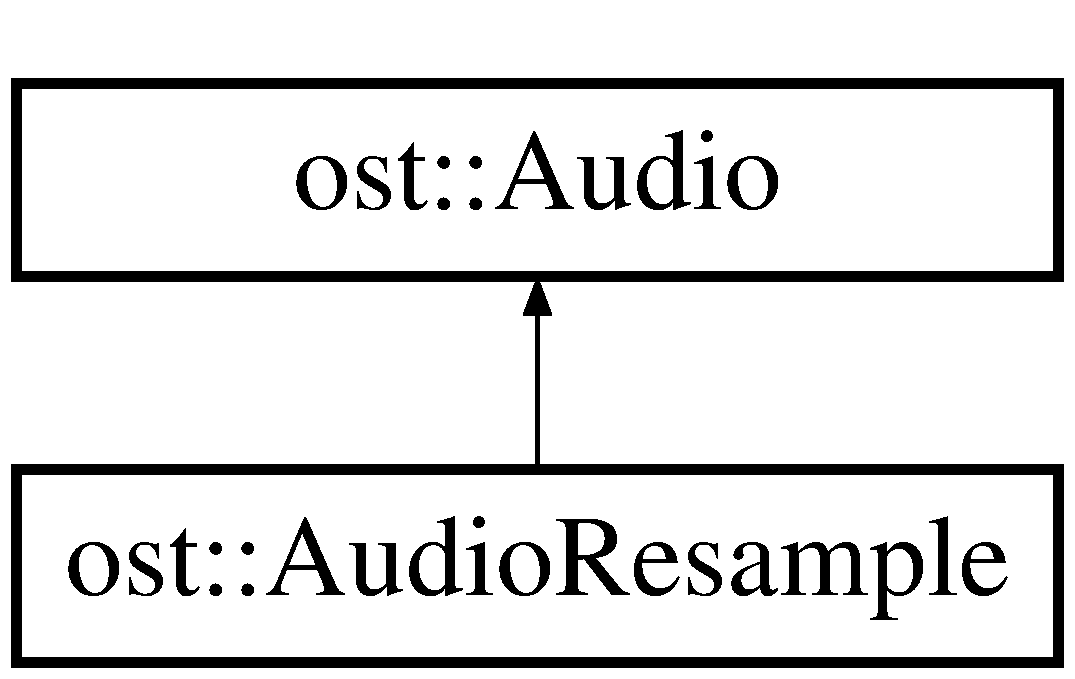
\includegraphics[height=2cm]{classost_1_1_audio_resample}
\end{center}
\end{figure}
\subsection*{Public Member Functions}
\begin{DoxyCompactItemize}
\item 
{\bf AudioResample} ({\bf Rate} mul, {\bf Rate} div)
\item 
{\bf $\sim$AudioResample} ()
\item 
size\_\-t {\bf process} ({\bf Linear} from, {\bf Linear} to, size\_\-t count)
\item 
size\_\-t {\bf estimate} (size\_\-t count)
\end{DoxyCompactItemize}
\subsection*{Protected Attributes}
\begin{DoxyCompactItemize}
\item 
unsigned {\bf mfact}
\item 
unsigned {\bf dfact}
\item 
unsigned {\bf max}
\item 
unsigned {\bf gpos}
\item 
unsigned {\bf ppos}
\item 
{\bf Sample} {\bf last}
\item 
{\bf Linear} {\bf buffer}
\end{DoxyCompactItemize}


\subsection{Detailed Description}
The \doxyref{AudioResample}{p.}{classost_1_1_audio_resample} class is used to manage linear intropolation buffering for rate conversions. \begin{DoxyAuthor}{Author}
David Sugar $<${\tt dyfet@ostel.com}$>$ linear intropolation and rate conversion. 
\end{DoxyAuthor}


\subsection{Constructor \& Destructor Documentation}
\index{ost::AudioResample@{ost::AudioResample}!AudioResample@{AudioResample}}
\index{AudioResample@{AudioResample}!ost::AudioResample@{ost::AudioResample}}
\subsubsection[{AudioResample}]{\setlength{\rightskip}{0pt plus 5cm}ost::AudioResample::AudioResample ({\bf Rate} {\em mul}, \/  {\bf Rate} {\em div})}\label{classost_1_1_audio_resample_a408740221daffc47f7a651b63c8b5c73}
\index{ost::AudioResample@{ost::AudioResample}!$\sim$AudioResample@{$\sim$AudioResample}}
\index{$\sim$AudioResample@{$\sim$AudioResample}!ost::AudioResample@{ost::AudioResample}}
\subsubsection[{$\sim$AudioResample}]{\setlength{\rightskip}{0pt plus 5cm}ost::AudioResample::$\sim$AudioResample ()}\label{classost_1_1_audio_resample_a9e64615c7cf798286195e0ac3071fdc1}


\subsection{Member Function Documentation}
\index{ost::AudioResample@{ost::AudioResample}!estimate@{estimate}}
\index{estimate@{estimate}!ost::AudioResample@{ost::AudioResample}}
\subsubsection[{estimate}]{\setlength{\rightskip}{0pt plus 5cm}size\_\-t ost::AudioResample::estimate (size\_\-t {\em count})}\label{classost_1_1_audio_resample_a27baa7b1cfec1cf55eaa5038208f9c28}
\index{ost::AudioResample@{ost::AudioResample}!process@{process}}
\index{process@{process}!ost::AudioResample@{ost::AudioResample}}
\subsubsection[{process}]{\setlength{\rightskip}{0pt plus 5cm}size\_\-t ost::AudioResample::process ({\bf Linear} {\em from}, \/  {\bf Linear} {\em to}, \/  size\_\-t {\em count})}\label{classost_1_1_audio_resample_af0bdd5ac2f0850324d048ecf86d02cc1}


\subsection{Member Data Documentation}
\index{ost::AudioResample@{ost::AudioResample}!buffer@{buffer}}
\index{buffer@{buffer}!ost::AudioResample@{ost::AudioResample}}
\subsubsection[{buffer}]{\setlength{\rightskip}{0pt plus 5cm}{\bf Linear} {\bf ost::AudioResample::buffer}\hspace{0.3cm}{\ttfamily  [protected]}}\label{classost_1_1_audio_resample_aa0c196fe38dc3512b3a8667082878e3f}
\index{ost::AudioResample@{ost::AudioResample}!dfact@{dfact}}
\index{dfact@{dfact}!ost::AudioResample@{ost::AudioResample}}
\subsubsection[{dfact}]{\setlength{\rightskip}{0pt plus 5cm}unsigned {\bf ost::AudioResample::dfact}\hspace{0.3cm}{\ttfamily  [protected]}}\label{classost_1_1_audio_resample_a8baae81f9d216302031b0934b8f2c0e4}
\index{ost::AudioResample@{ost::AudioResample}!gpos@{gpos}}
\index{gpos@{gpos}!ost::AudioResample@{ost::AudioResample}}
\subsubsection[{gpos}]{\setlength{\rightskip}{0pt plus 5cm}unsigned {\bf ost::AudioResample::gpos}\hspace{0.3cm}{\ttfamily  [protected]}}\label{classost_1_1_audio_resample_a03c347a6d21f77f94c7703030c983b67}
\index{ost::AudioResample@{ost::AudioResample}!last@{last}}
\index{last@{last}!ost::AudioResample@{ost::AudioResample}}
\subsubsection[{last}]{\setlength{\rightskip}{0pt plus 5cm}{\bf Sample} {\bf ost::AudioResample::last}\hspace{0.3cm}{\ttfamily  [protected]}}\label{classost_1_1_audio_resample_a239a00ff4ef4eca85ecb134804e6e9b2}
\index{ost::AudioResample@{ost::AudioResample}!max@{max}}
\index{max@{max}!ost::AudioResample@{ost::AudioResample}}
\subsubsection[{max}]{\setlength{\rightskip}{0pt plus 5cm}unsigned {\bf ost::AudioResample::max}\hspace{0.3cm}{\ttfamily  [protected]}}\label{classost_1_1_audio_resample_a96c78af7fc79e221815873acae145b72}
\index{ost::AudioResample@{ost::AudioResample}!mfact@{mfact}}
\index{mfact@{mfact}!ost::AudioResample@{ost::AudioResample}}
\subsubsection[{mfact}]{\setlength{\rightskip}{0pt plus 5cm}unsigned {\bf ost::AudioResample::mfact}\hspace{0.3cm}{\ttfamily  [protected]}}\label{classost_1_1_audio_resample_a986ef6a994491b684ee5664b373698bf}
\index{ost::AudioResample@{ost::AudioResample}!ppos@{ppos}}
\index{ppos@{ppos}!ost::AudioResample@{ost::AudioResample}}
\subsubsection[{ppos}]{\setlength{\rightskip}{0pt plus 5cm}unsigned {\bf ost::AudioResample::ppos}\hspace{0.3cm}{\ttfamily  [protected]}}\label{classost_1_1_audio_resample_a1ebaf6e154b47bb2f28266d256c699da}


The documentation for this class was generated from the following file:\begin{DoxyCompactItemize}
\item 
{\bf audio2.h}\end{DoxyCompactItemize}

\section{ost::AudioStream Class Reference}
\label{classost_1_1_audio_stream}\index{ost::AudioStream@{ost::AudioStream}}


\doxyref{AudioStream}{p.}{classost_1_1_audio_stream} accesses \doxyref{AudioFile}{p.}{classost_1_1_audio_file} base class content as fixed frames of streaming linear samples.  


{\ttfamily \#include $<$audio2.h$>$}Inheritance diagram for ost::AudioStream::\begin{figure}[H]
\begin{center}
\leavevmode
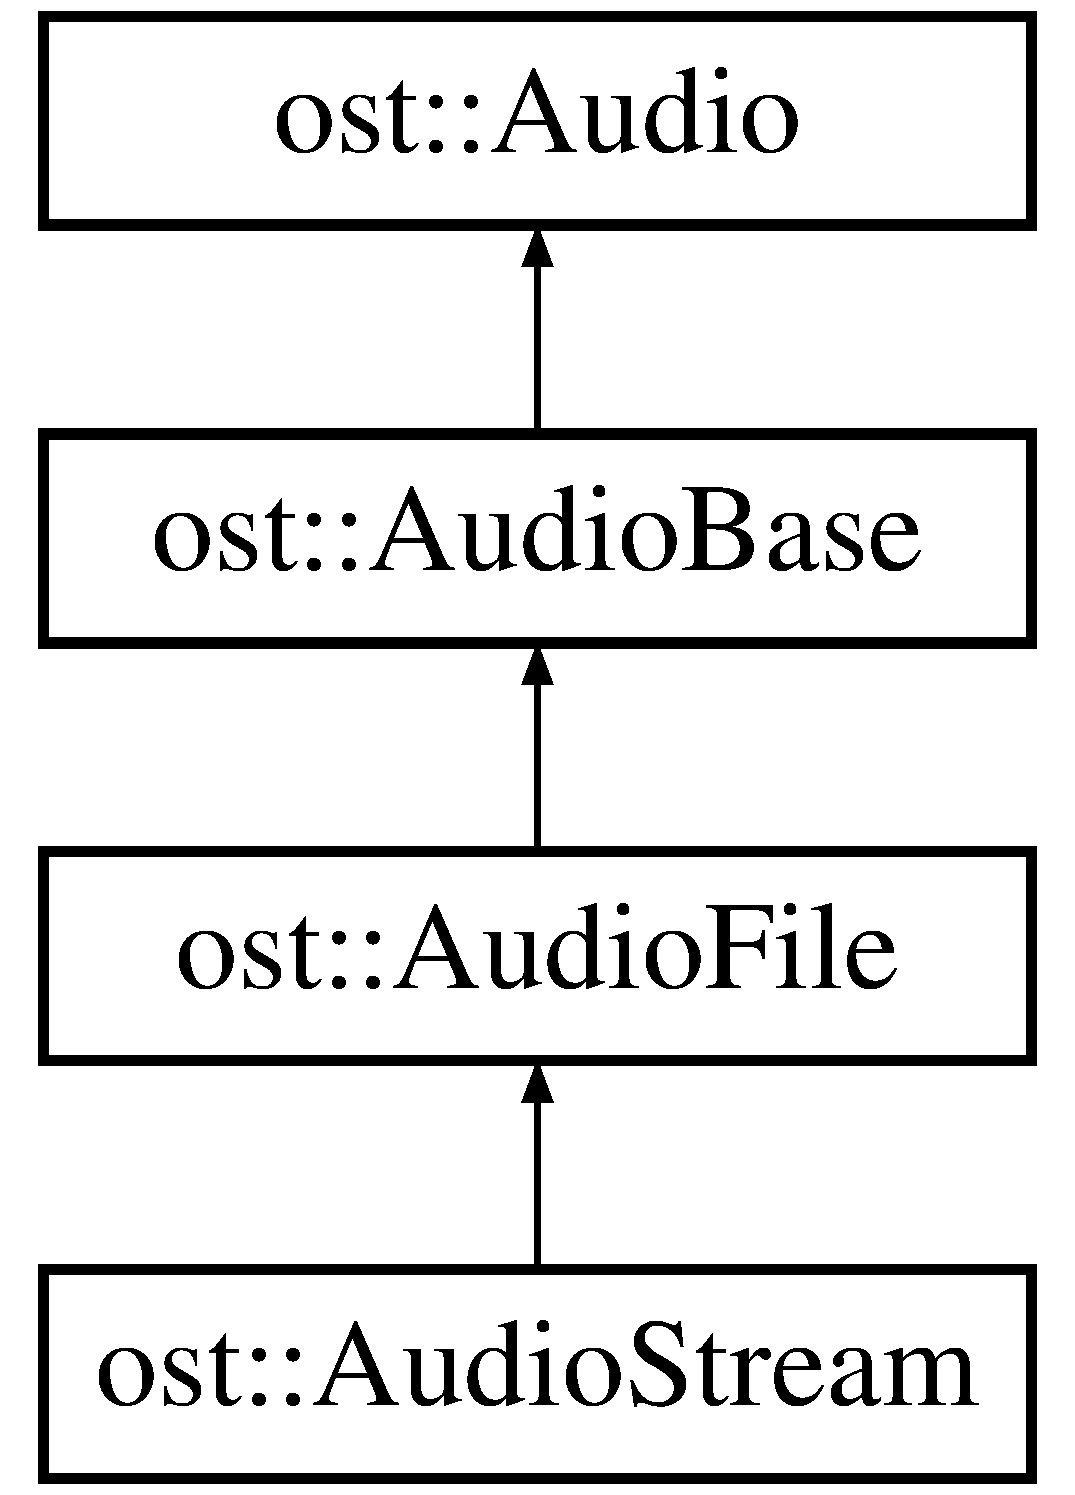
\includegraphics[height=4cm]{classost_1_1_audio_stream}
\end{center}
\end{figure}
\subsection*{Public Member Functions}
\begin{DoxyCompactItemize}
\item 
{\bf AudioStream} ()
\begin{DoxyCompactList}\small\item\em Create a new audiostream object. \item\end{DoxyCompactList}\item 
{\bf AudioStream} (const char $\ast$name, {\bf Mode} {\bf mode}=modeRead, {\bf timeout\_\-t} framing=0)
\begin{DoxyCompactList}\small\item\em Create an audio stream object and open an existing audio file. \item\end{DoxyCompactList}\item 
{\bf AudioStream} (const char $\ast$name, {\bf Info} $\ast${\bf info}, bool exclusive=false, {\bf timeout\_\-t} framing=0)
\begin{DoxyCompactList}\small\item\em Create an audio stream object and a new audio file. \item\end{DoxyCompactList}\item 
virtual {\bf $\sim$AudioStream} ()
\item 
ssize\_\-t {\bf getBuffer} ({\bf Encoded} data, size\_\-t count)
\begin{DoxyCompactList}\small\item\em Virtual for packet i/o intercept. \item\end{DoxyCompactList}\item 
void {\bf open} (const char $\ast$name, {\bf Mode} {\bf mode}=modeRead, {\bf timeout\_\-t} framing=0)
\begin{DoxyCompactList}\small\item\em Open existing audio file for streaming. \item\end{DoxyCompactList}\item 
void {\bf create} (const char $\ast$name, {\bf Info} $\ast${\bf info}, bool exclusive=false, {\bf timeout\_\-t} framing=0)
\begin{DoxyCompactList}\small\item\em Create a new audio file for streaming. \item\end{DoxyCompactList}\item 
void {\bf close} (void)
\begin{DoxyCompactList}\small\item\em Close the currently open audio file for streaming. \item\end{DoxyCompactList}\item 
void {\bf flush} (void)
\begin{DoxyCompactList}\small\item\em flush any unsaved buffered data to disk. \item\end{DoxyCompactList}\item 
bool {\bf isStreamable} (void)
\begin{DoxyCompactList}\small\item\em Check if the audio file may be streamed. \item\end{DoxyCompactList}\item 
unsigned {\bf getCount} (void)
\begin{DoxyCompactList}\small\item\em Get the number of samples expected in a frame. \item\end{DoxyCompactList}\item 
unsigned {\bf getEncoded} ({\bf AudioCodec} $\ast${\bf codec}, {\bf Encoded} address, unsigned frames=1)
\begin{DoxyCompactList}\small\item\em Stream audio data from the file and convert into an alternate encoding based on the codec supplied. \item\end{DoxyCompactList}\item 
unsigned {\bf putEncoded} ({\bf AudioCodec} $\ast${\bf codec}, {\bf Encoded} address, unsigned frames=1)
\begin{DoxyCompactList}\small\item\em Stream audio data in an alternate codec into the currently opened file. \item\end{DoxyCompactList}\item 
unsigned {\bf getEncoded} ({\bf Encoded} address, unsigned frames=1)
\begin{DoxyCompactList}\small\item\em Get data from the streamed file in it's native encoding. \item\end{DoxyCompactList}\item 
unsigned {\bf putEncoded} ({\bf Encoded} address, unsigned frames=1)
\begin{DoxyCompactList}\small\item\em Put data encoded in the native format of the stream file. \item\end{DoxyCompactList}\item 
ssize\_\-t {\bf getPacket} ({\bf Encoded} data)
\begin{DoxyCompactList}\small\item\em Get a packet of data from the file. \item\end{DoxyCompactList}\item 
unsigned {\bf getMono} ({\bf Linear} buffer, unsigned frames=1)
\begin{DoxyCompactList}\small\item\em Get and automatically convert audio file data into mono linear audio samples. \item\end{DoxyCompactList}\item 
unsigned {\bf getStereo} ({\bf Linear} buffer, unsigned frames=1)
\begin{DoxyCompactList}\small\item\em Get and automatically convert audio file data into stereo (two channel) linear audio samples. \item\end{DoxyCompactList}\item 
unsigned {\bf putMono} ({\bf Linear} buffer, unsigned frames=1)
\begin{DoxyCompactList}\small\item\em Automatically convert and put mono linear audio data into the audio file. \item\end{DoxyCompactList}\item 
unsigned {\bf putStereo} ({\bf Linear} buffer, unsigned frames=1)
\begin{DoxyCompactList}\small\item\em Automatically convert and put stereo linear audio data into the audio file. \item\end{DoxyCompactList}\item 
unsigned {\bf bufMono} ({\bf Linear} buffer, unsigned count)
\begin{DoxyCompactList}\small\item\em Automatically convert and put arbitrary linear mono data into the audio file. \item\end{DoxyCompactList}\item 
unsigned {\bf bufStereo} ({\bf Linear} buffer, unsigned count)
\begin{DoxyCompactList}\small\item\em Automatically convert and put arbitrary linear stereo data into the audio file. \item\end{DoxyCompactList}\item 
{\bf AudioCodec} $\ast$ {\bf getCodec} (void)
\begin{DoxyCompactList}\small\item\em Return the codec being used if there is one. \item\end{DoxyCompactList}\end{DoxyCompactItemize}
\subsection*{Protected Member Functions}
\begin{DoxyCompactItemize}
\item 
unsigned {\bf bufAudio} ({\bf Linear} samples, unsigned count, unsigned size)
\end{DoxyCompactItemize}
\subsection*{Protected Attributes}
\begin{DoxyCompactItemize}
\item 
{\bf AudioCodec} $\ast$ {\bf codec}
\item 
{\bf Encoded} {\bf framebuf}
\item 
bool {\bf streamable}
\item 
{\bf Linear} {\bf bufferFrame}
\item 
unsigned {\bf bufferPosition}
\item 
unsigned {\bf bufferChannels}
\item 
{\bf Linear} {\bf encBuffer}
\item 
{\bf Linear} {\bf decBuffer}
\item 
unsigned {\bf encSize}
\item 
unsigned {\bf decSize}
\end{DoxyCompactItemize}


\subsection{Detailed Description}
\doxyref{AudioStream}{p.}{classost_1_1_audio_stream} accesses \doxyref{AudioFile}{p.}{classost_1_1_audio_file} base class content as fixed frames of streaming linear samples. If a codec must be assigned to perform conversion to/from linear data, \doxyref{AudioStream}{p.}{classost_1_1_audio_stream} will handle conversion automatically. \doxyref{AudioStream}{p.}{classost_1_1_audio_stream} will also convert between mono and stereo audio content. \doxyref{AudioStream}{p.}{classost_1_1_audio_stream} uses linear samples in the native machine endian format and perform endian byte swapping as needed.

\begin{DoxyAuthor}{Author}
David Sugar $<${\tt dyfet@ostel.com}$>$ \doxyref{Audio}{p.}{classost_1_1_audio} Streaming with Linear Conversion 
\end{DoxyAuthor}


\subsection{Constructor \& Destructor Documentation}
\index{ost::AudioStream@{ost::AudioStream}!AudioStream@{AudioStream}}
\index{AudioStream@{AudioStream}!ost::AudioStream@{ost::AudioStream}}
\subsubsection[{AudioStream}]{\setlength{\rightskip}{0pt plus 5cm}ost::AudioStream::AudioStream ()}\label{classost_1_1_audio_stream_ae7c476840e97627aec743f0224aad1fe}


Create a new audiostream object. \index{ost::AudioStream@{ost::AudioStream}!AudioStream@{AudioStream}}
\index{AudioStream@{AudioStream}!ost::AudioStream@{ost::AudioStream}}
\subsubsection[{AudioStream}]{\setlength{\rightskip}{0pt plus 5cm}ost::AudioStream::AudioStream (const char $\ast$ {\em name}, \/  {\bf Mode} {\em mode} = {\ttfamily modeRead}, \/  {\bf timeout\_\-t} {\em framing} = {\ttfamily 0})}\label{classost_1_1_audio_stream_ab67af760e72849a25898e18e2edf8fea}


Create an audio stream object and open an existing audio file. 
\begin{DoxyParams}{Parameters}
\item[{\em name}]of file to open. \item[{\em mode}]of file access. \item[{\em framing}]time in milliseconds. \end{DoxyParams}
\index{ost::AudioStream@{ost::AudioStream}!AudioStream@{AudioStream}}
\index{AudioStream@{AudioStream}!ost::AudioStream@{ost::AudioStream}}
\subsubsection[{AudioStream}]{\setlength{\rightskip}{0pt plus 5cm}ost::AudioStream::AudioStream (const char $\ast$ {\em name}, \/  {\bf Info} $\ast$ {\em info}, \/  bool {\em exclusive} = {\ttfamily false}, \/  {\bf timeout\_\-t} {\em framing} = {\ttfamily 0})}\label{classost_1_1_audio_stream_a3ca0f83adf5bd721a86fa26710c6e338}


Create an audio stream object and a new audio file. 
\begin{DoxyParams}{Parameters}
\item[{\em name}]of file to open. \item[{\em info}]source description for properties of new file. \item[{\em exclusive}]access if true. \item[{\em framing}]time in milliseconds. \end{DoxyParams}
\index{ost::AudioStream@{ost::AudioStream}!$\sim$AudioStream@{$\sim$AudioStream}}
\index{$\sim$AudioStream@{$\sim$AudioStream}!ost::AudioStream@{ost::AudioStream}}
\subsubsection[{$\sim$AudioStream}]{\setlength{\rightskip}{0pt plus 5cm}virtual ost::AudioStream::$\sim$AudioStream ()\hspace{0.3cm}{\ttfamily  [virtual]}}\label{classost_1_1_audio_stream_a2224c65e284690dd924af3f1f2f24630}


\subsection{Member Function Documentation}
\index{ost::AudioStream@{ost::AudioStream}!bufAudio@{bufAudio}}
\index{bufAudio@{bufAudio}!ost::AudioStream@{ost::AudioStream}}
\subsubsection[{bufAudio}]{\setlength{\rightskip}{0pt plus 5cm}unsigned ost::AudioStream::bufAudio ({\bf Linear} {\em samples}, \/  unsigned {\em count}, \/  unsigned {\em size})\hspace{0.3cm}{\ttfamily  [protected]}}\label{classost_1_1_audio_stream_adab79077d903b00da35240fdeaeadf16}
\index{ost::AudioStream@{ost::AudioStream}!bufMono@{bufMono}}
\index{bufMono@{bufMono}!ost::AudioStream@{ost::AudioStream}}
\subsubsection[{bufMono}]{\setlength{\rightskip}{0pt plus 5cm}unsigned ost::AudioStream::bufMono ({\bf Linear} {\em buffer}, \/  unsigned {\em count})}\label{classost_1_1_audio_stream_aa4c33abc46eedf00c9a061130185bffe}


Automatically convert and put arbitrary linear mono data into the audio file. Convert to stereo and buffer incomplete frames as needed by the streaming file.


\begin{DoxyParams}{Parameters}
\item[{\em buffer}]to save linear audio from. \item[{\em count}]of linear audio to write. \end{DoxyParams}
\begin{DoxyReturn}{Returns}
number of linear audio samples written to file. 
\end{DoxyReturn}
\index{ost::AudioStream@{ost::AudioStream}!bufStereo@{bufStereo}}
\index{bufStereo@{bufStereo}!ost::AudioStream@{ost::AudioStream}}
\subsubsection[{bufStereo}]{\setlength{\rightskip}{0pt plus 5cm}unsigned ost::AudioStream::bufStereo ({\bf Linear} {\em buffer}, \/  unsigned {\em count})}\label{classost_1_1_audio_stream_afd95f7a2df57101f7773920528c61abb}


Automatically convert and put arbitrary linear stereo data into the audio file. Convert to mono and buffer incomplete frames as needed by the streaming file.


\begin{DoxyParams}{Parameters}
\item[{\em buffer}]to save linear audio from. \item[{\em count}]of linear audio to write. \end{DoxyParams}
\begin{DoxyReturn}{Returns}
number of linear audio samples written to file. 
\end{DoxyReturn}
\index{ost::AudioStream@{ost::AudioStream}!close@{close}}
\index{close@{close}!ost::AudioStream@{ost::AudioStream}}
\subsubsection[{close}]{\setlength{\rightskip}{0pt plus 5cm}void ost::AudioStream::close (void)}\label{classost_1_1_audio_stream_a823bf9a3d64dbae7117b6c29681017d3}


Close the currently open audio file for streaming. 

Reimplemented from {\bf ost::AudioFile} \doxyref{}{p.}{classost_1_1_audio_file_aba0e5a66e006c61aef1ddbd018e2e7ed}.\index{ost::AudioStream@{ost::AudioStream}!create@{create}}
\index{create@{create}!ost::AudioStream@{ost::AudioStream}}
\subsubsection[{create}]{\setlength{\rightskip}{0pt plus 5cm}void ost::AudioStream::create (const char $\ast$ {\em name}, \/  {\bf Info} $\ast$ {\em info}, \/  bool {\em exclusive} = {\ttfamily false}, \/  {\bf timeout\_\-t} {\em framing} = {\ttfamily 0})}\label{classost_1_1_audio_stream_a58fd6f03aff924fdd330919caf543623}


Create a new audio file for streaming. 
\begin{DoxyParams}{Parameters}
\item[{\em name}]of file to create. \item[{\em info}]source description for file properties. \item[{\em exclusive}]true for exclusive access. \item[{\em framing}]timing in milliseconds. \end{DoxyParams}


Reimplemented from {\bf ost::AudioFile} \doxyref{}{p.}{classost_1_1_audio_file_af536da5d45926c3f75075c76f12ecb51}.\index{ost::AudioStream@{ost::AudioStream}!flush@{flush}}
\index{flush@{flush}!ost::AudioStream@{ost::AudioStream}}
\subsubsection[{flush}]{\setlength{\rightskip}{0pt plus 5cm}void ost::AudioStream::flush (void)}\label{classost_1_1_audio_stream_a0c1c16d1db4e4a9d6d6a06eb0fa98f71}


flush any unsaved buffered data to disk. \index{ost::AudioStream@{ost::AudioStream}!getBuffer@{getBuffer}}
\index{getBuffer@{getBuffer}!ost::AudioStream@{ost::AudioStream}}
\subsubsection[{getBuffer}]{\setlength{\rightskip}{0pt plus 5cm}ssize\_\-t ost::AudioStream::getBuffer ({\bf Encoded} {\em data}, \/  size\_\-t {\em count})\hspace{0.3cm}{\ttfamily  [virtual]}}\label{classost_1_1_audio_stream_a32945278bd2fcb2b03c97f15d78f571b}


Virtual for packet i/o intercept. \begin{DoxyReturn}{Returns}
bytes read. 
\end{DoxyReturn}

\begin{DoxyParams}{Parameters}
\item[{\em data}]encoding buffer. \item[{\em count}]requested. \end{DoxyParams}


Reimplemented from {\bf ost::AudioFile} \doxyref{}{p.}{classost_1_1_audio_file_a40e6fcddf43df289fef2f66ccbe84bbd}.\index{ost::AudioStream@{ost::AudioStream}!getCodec@{getCodec}}
\index{getCodec@{getCodec}!ost::AudioStream@{ost::AudioStream}}
\subsubsection[{getCodec}]{\setlength{\rightskip}{0pt plus 5cm}{\bf AudioCodec}$\ast$ ost::AudioStream::getCodec (void)\hspace{0.3cm}{\ttfamily  [inline]}}\label{classost_1_1_audio_stream_a47823d4a7bc81c6fd488af7df15ed755}


Return the codec being used if there is one. \begin{DoxyReturn}{Returns}
codec used. 
\end{DoxyReturn}


Reimplemented from {\bf ost::AudioFile} \doxyref{}{p.}{classost_1_1_audio_file_a5a2a7d99d0b81e72b88cea73294de33b}.\index{ost::AudioStream@{ost::AudioStream}!getCount@{getCount}}
\index{getCount@{getCount}!ost::AudioStream@{ost::AudioStream}}
\subsubsection[{getCount}]{\setlength{\rightskip}{0pt plus 5cm}unsigned ost::AudioStream::getCount (void)}\label{classost_1_1_audio_stream_a3aa469beded2aed7ce2e6931171db597}


Get the number of samples expected in a frame. \index{ost::AudioStream@{ost::AudioStream}!getEncoded@{getEncoded}}
\index{getEncoded@{getEncoded}!ost::AudioStream@{ost::AudioStream}}
\subsubsection[{getEncoded}]{\setlength{\rightskip}{0pt plus 5cm}unsigned ost::AudioStream::getEncoded ({\bf Encoded} {\em address}, \/  unsigned {\em frames} = {\ttfamily 1})}\label{classost_1_1_audio_stream_a2da57851f76ca5a358638d46d6e6887e}


Get data from the streamed file in it's native encoding. 
\begin{DoxyParams}{Parameters}
\item[{\em address}]to save encoded audio. \item[{\em frames}]of audio to load. \end{DoxyParams}
\begin{DoxyReturn}{Returns}
number of frames read. 
\end{DoxyReturn}
\index{ost::AudioStream@{ost::AudioStream}!getEncoded@{getEncoded}}
\index{getEncoded@{getEncoded}!ost::AudioStream@{ost::AudioStream}}
\subsubsection[{getEncoded}]{\setlength{\rightskip}{0pt plus 5cm}unsigned ost::AudioStream::getEncoded ({\bf AudioCodec} $\ast$ {\em codec}, \/  {\bf Encoded} {\em address}, \/  unsigned {\em frames} = {\ttfamily 1})}\label{classost_1_1_audio_stream_a98d814ef2eb3e646f22f3ef36fa47f34}


Stream audio data from the file and convert into an alternate encoding based on the codec supplied. 
\begin{DoxyParams}{Parameters}
\item[{\em codec}]to apply before saving. \item[{\em address}]of data to save. \item[{\em frames}]to stream by the codec. \end{DoxyParams}
\begin{DoxyReturn}{Returns}
number of frames processed. 
\end{DoxyReturn}
\index{ost::AudioStream@{ost::AudioStream}!getMono@{getMono}}
\index{getMono@{getMono}!ost::AudioStream@{ost::AudioStream}}
\subsubsection[{getMono}]{\setlength{\rightskip}{0pt plus 5cm}unsigned ost::AudioStream::getMono ({\bf Linear} {\em buffer}, \/  unsigned {\em frames} = {\ttfamily 1})}\label{classost_1_1_audio_stream_a6d17c9a029b0ac28148eb9107acff751}


Get and automatically convert audio file data into mono linear audio samples. 
\begin{DoxyParams}{Parameters}
\item[{\em buffer}]to save linear audio into. \item[{\em frames}]of audio to read. \end{DoxyParams}
\begin{DoxyReturn}{Returns}
number of frames read from file. 
\end{DoxyReturn}
\index{ost::AudioStream@{ost::AudioStream}!getPacket@{getPacket}}
\index{getPacket@{getPacket}!ost::AudioStream@{ost::AudioStream}}
\subsubsection[{getPacket}]{\setlength{\rightskip}{0pt plus 5cm}ssize\_\-t ost::AudioStream::getPacket ({\bf Encoded} {\em data})}\label{classost_1_1_audio_stream_aab3a8568a6e1b3c9660a6c63b049ccd6}


Get a packet of data from the file. This uses the codec to determine what a true packet boundry is.


\begin{DoxyParams}{Parameters}
\item[{\em buffer}]to save encoded data. \end{DoxyParams}
\begin{DoxyReturn}{Returns}
number of bytes read as packet. 
\end{DoxyReturn}


Reimplemented from {\bf ost::AudioBase} \doxyref{}{p.}{classost_1_1_audio_base_a26a26fef0bcc5a158dab9cdf5a0d772e}.\index{ost::AudioStream@{ost::AudioStream}!getStereo@{getStereo}}
\index{getStereo@{getStereo}!ost::AudioStream@{ost::AudioStream}}
\subsubsection[{getStereo}]{\setlength{\rightskip}{0pt plus 5cm}unsigned ost::AudioStream::getStereo ({\bf Linear} {\em buffer}, \/  unsigned {\em frames} = {\ttfamily 1})}\label{classost_1_1_audio_stream_a287e2a936022552de4f8bc7731df3bba}


Get and automatically convert audio file data into stereo (two channel) linear audio samples. 
\begin{DoxyParams}{Parameters}
\item[{\em buffer}]to save linear audio into. \item[{\em frames}]of audio to read. \end{DoxyParams}
\begin{DoxyReturn}{Returns}
number of frames read from file. 
\end{DoxyReturn}
\index{ost::AudioStream@{ost::AudioStream}!isStreamable@{isStreamable}}
\index{isStreamable@{isStreamable}!ost::AudioStream@{ost::AudioStream}}
\subsubsection[{isStreamable}]{\setlength{\rightskip}{0pt plus 5cm}bool ost::AudioStream::isStreamable (void)}\label{classost_1_1_audio_stream_aaf520ef6e2e3da00c0d0cfc4eee781ea}


Check if the audio file may be streamed. Files can be streamed if a codec is available or if they are linear.

\begin{DoxyReturn}{Returns}
true if streamable. 
\end{DoxyReturn}
\index{ost::AudioStream@{ost::AudioStream}!open@{open}}
\index{open@{open}!ost::AudioStream@{ost::AudioStream}}
\subsubsection[{open}]{\setlength{\rightskip}{0pt plus 5cm}void ost::AudioStream::open (const char $\ast$ {\em name}, \/  {\bf Mode} {\em mode} = {\ttfamily modeRead}, \/  {\bf timeout\_\-t} {\em framing} = {\ttfamily 0})}\label{classost_1_1_audio_stream_a2dba2a15630314e4eb6a134ca82b5a60}


Open existing audio file for streaming. 
\begin{DoxyParams}{Parameters}
\item[{\em name}]of file to open. \item[{\em mode}]to use file. \item[{\em framing}]timer in milliseconds. \end{DoxyParams}


Reimplemented from {\bf ost::AudioFile} \doxyref{}{p.}{classost_1_1_audio_file_a6aa46c6af42e7155be4f92d1b7e0109b}.\index{ost::AudioStream@{ost::AudioStream}!putEncoded@{putEncoded}}
\index{putEncoded@{putEncoded}!ost::AudioStream@{ost::AudioStream}}
\subsubsection[{putEncoded}]{\setlength{\rightskip}{0pt plus 5cm}unsigned ost::AudioStream::putEncoded ({\bf Encoded} {\em address}, \/  unsigned {\em frames} = {\ttfamily 1})}\label{classost_1_1_audio_stream_a4b6bd9cfec637f8717956a307a29c3cc}


Put data encoded in the native format of the stream file. 
\begin{DoxyParams}{Parameters}
\item[{\em address}]to load encoded audio. \item[{\em frames}]of audio to save. \end{DoxyParams}
\begin{DoxyReturn}{Returns}
number of frames written. 
\end{DoxyReturn}
\index{ost::AudioStream@{ost::AudioStream}!putEncoded@{putEncoded}}
\index{putEncoded@{putEncoded}!ost::AudioStream@{ost::AudioStream}}
\subsubsection[{putEncoded}]{\setlength{\rightskip}{0pt plus 5cm}unsigned ost::AudioStream::putEncoded ({\bf AudioCodec} $\ast$ {\em codec}, \/  {\bf Encoded} {\em address}, \/  unsigned {\em frames} = {\ttfamily 1})}\label{classost_1_1_audio_stream_a80bdb4f5e1b1f21206305592745b4556}


Stream audio data in an alternate codec into the currently opened file. 
\begin{DoxyParams}{Parameters}
\item[{\em codec}]to convert incoming data from. \item[{\em address}]of data to convert and stream. \item[{\em frames}]of audio to stream. \end{DoxyParams}
\begin{DoxyReturn}{Returns}
number of frames processed. 
\end{DoxyReturn}
\index{ost::AudioStream@{ost::AudioStream}!putMono@{putMono}}
\index{putMono@{putMono}!ost::AudioStream@{ost::AudioStream}}
\subsubsection[{putMono}]{\setlength{\rightskip}{0pt plus 5cm}unsigned ost::AudioStream::putMono ({\bf Linear} {\em buffer}, \/  unsigned {\em frames} = {\ttfamily 1})}\label{classost_1_1_audio_stream_a1dc042d6cdea238dd371d447103dca3a}


Automatically convert and put mono linear audio data into the audio file. Convert to stereo as needed by file format.


\begin{DoxyParams}{Parameters}
\item[{\em buffer}]to save linear audio from. \item[{\em frames}]of audio to write. \end{DoxyParams}
\begin{DoxyReturn}{Returns}
number of frames written to file. 
\end{DoxyReturn}
\index{ost::AudioStream@{ost::AudioStream}!putStereo@{putStereo}}
\index{putStereo@{putStereo}!ost::AudioStream@{ost::AudioStream}}
\subsubsection[{putStereo}]{\setlength{\rightskip}{0pt plus 5cm}unsigned ost::AudioStream::putStereo ({\bf Linear} {\em buffer}, \/  unsigned {\em frames} = {\ttfamily 1})}\label{classost_1_1_audio_stream_a5f9d1dbc5dce59b1307546931718f561}


Automatically convert and put stereo linear audio data into the audio file. Convert to mono as needed by file format.


\begin{DoxyParams}{Parameters}
\item[{\em buffer}]to save linear audio from. \item[{\em frames}]of audio to write. \end{DoxyParams}
\begin{DoxyReturn}{Returns}
number of frames written to file. 
\end{DoxyReturn}


\subsection{Member Data Documentation}
\index{ost::AudioStream@{ost::AudioStream}!bufferChannels@{bufferChannels}}
\index{bufferChannels@{bufferChannels}!ost::AudioStream@{ost::AudioStream}}
\subsubsection[{bufferChannels}]{\setlength{\rightskip}{0pt plus 5cm}unsigned {\bf ost::AudioStream::bufferChannels}\hspace{0.3cm}{\ttfamily  [protected]}}\label{classost_1_1_audio_stream_a523ae30758d099f93c2d4036fcb25fdf}
\index{ost::AudioStream@{ost::AudioStream}!bufferFrame@{bufferFrame}}
\index{bufferFrame@{bufferFrame}!ost::AudioStream@{ost::AudioStream}}
\subsubsection[{bufferFrame}]{\setlength{\rightskip}{0pt plus 5cm}{\bf Linear} {\bf ost::AudioStream::bufferFrame}\hspace{0.3cm}{\ttfamily  [protected]}}\label{classost_1_1_audio_stream_a0735cc187829f8cb3f4b44df94db5ed2}
\index{ost::AudioStream@{ost::AudioStream}!bufferPosition@{bufferPosition}}
\index{bufferPosition@{bufferPosition}!ost::AudioStream@{ost::AudioStream}}
\subsubsection[{bufferPosition}]{\setlength{\rightskip}{0pt plus 5cm}unsigned {\bf ost::AudioStream::bufferPosition}\hspace{0.3cm}{\ttfamily  [protected]}}\label{classost_1_1_audio_stream_ac43e4053dba97120a826df030025e767}
\index{ost::AudioStream@{ost::AudioStream}!codec@{codec}}
\index{codec@{codec}!ost::AudioStream@{ost::AudioStream}}
\subsubsection[{codec}]{\setlength{\rightskip}{0pt plus 5cm}{\bf AudioCodec}$\ast$ {\bf ost::AudioStream::codec}\hspace{0.3cm}{\ttfamily  [protected]}}\label{classost_1_1_audio_stream_a36d87f56ca6a25e8e477cf98c559c5a6}
\index{ost::AudioStream@{ost::AudioStream}!decBuffer@{decBuffer}}
\index{decBuffer@{decBuffer}!ost::AudioStream@{ost::AudioStream}}
\subsubsection[{decBuffer}]{\setlength{\rightskip}{0pt plus 5cm}{\bf Linear} {\bf ost::AudioStream::decBuffer}\hspace{0.3cm}{\ttfamily  [protected]}}\label{classost_1_1_audio_stream_aabc88921668e15b9eb20baa6906b4fdf}
\index{ost::AudioStream@{ost::AudioStream}!decSize@{decSize}}
\index{decSize@{decSize}!ost::AudioStream@{ost::AudioStream}}
\subsubsection[{decSize}]{\setlength{\rightskip}{0pt plus 5cm}unsigned {\bf ost::AudioStream::decSize}\hspace{0.3cm}{\ttfamily  [protected]}}\label{classost_1_1_audio_stream_a587b93ce80081042f0d49bc93b8afd1e}
\index{ost::AudioStream@{ost::AudioStream}!encBuffer@{encBuffer}}
\index{encBuffer@{encBuffer}!ost::AudioStream@{ost::AudioStream}}
\subsubsection[{encBuffer}]{\setlength{\rightskip}{0pt plus 5cm}{\bf Linear} {\bf ost::AudioStream::encBuffer}\hspace{0.3cm}{\ttfamily  [protected]}}\label{classost_1_1_audio_stream_aa602b11f03414d79135c93fde44c3e01}
\index{ost::AudioStream@{ost::AudioStream}!encSize@{encSize}}
\index{encSize@{encSize}!ost::AudioStream@{ost::AudioStream}}
\subsubsection[{encSize}]{\setlength{\rightskip}{0pt plus 5cm}unsigned {\bf ost::AudioStream::encSize}\hspace{0.3cm}{\ttfamily  [protected]}}\label{classost_1_1_audio_stream_a2efa96f577a5c2cfd9013b2dec4c17b1}
\index{ost::AudioStream@{ost::AudioStream}!framebuf@{framebuf}}
\index{framebuf@{framebuf}!ost::AudioStream@{ost::AudioStream}}
\subsubsection[{framebuf}]{\setlength{\rightskip}{0pt plus 5cm}{\bf Encoded} {\bf ost::AudioStream::framebuf}\hspace{0.3cm}{\ttfamily  [protected]}}\label{classost_1_1_audio_stream_afddcd59bb4f012dc5bb7d565750a1e5d}
\index{ost::AudioStream@{ost::AudioStream}!streamable@{streamable}}
\index{streamable@{streamable}!ost::AudioStream@{ost::AudioStream}}
\subsubsection[{streamable}]{\setlength{\rightskip}{0pt plus 5cm}bool {\bf ost::AudioStream::streamable}\hspace{0.3cm}{\ttfamily  [protected]}}\label{classost_1_1_audio_stream_a2457cfcde22eed8ee32152dd60039bd3}


The documentation for this class was generated from the following file:\begin{DoxyCompactItemize}
\item 
{\bf audio2.h}\end{DoxyCompactItemize}

\section{ost::AudioTone Class Reference}
\label{classost_1_1_audio_tone}\index{ost::AudioTone@{ost::AudioTone}}


The \doxyref{AudioTone}{p.}{classost_1_1_audio_tone} class is used to create a frame of audio encoded single or dualtones.  


{\ttfamily \#include $<$audio2.h$>$}Inheritance diagram for ost::AudioTone::\begin{figure}[H]
\begin{center}
\leavevmode
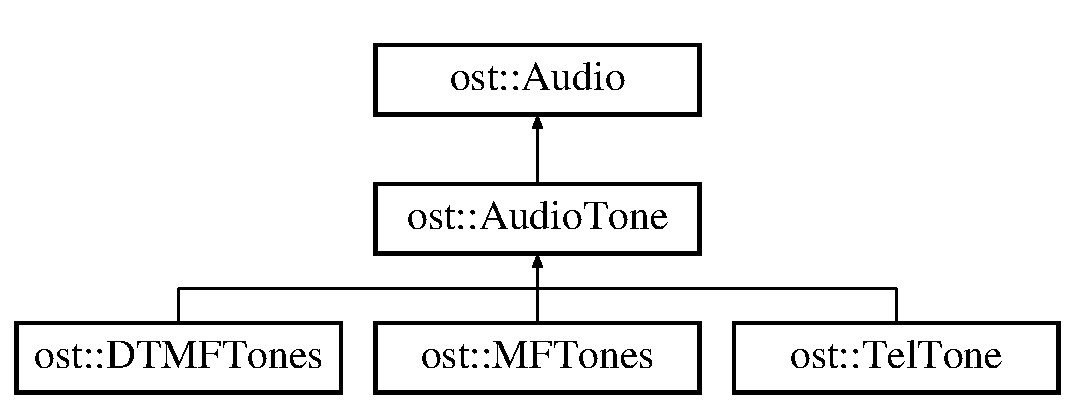
\includegraphics[height=3cm]{classost_1_1_audio_tone}
\end{center}
\end{figure}
\subsection*{Public Member Functions}
\begin{DoxyCompactItemize}
\item 
{\bf Rate} {\bf getRate} (void)
\begin{DoxyCompactList}\small\item\em Get the sample encoding rate being used for the tone generator. \item\end{DoxyCompactList}\item 
size\_\-t {\bf getSamples} (void)
\begin{DoxyCompactList}\small\item\em Get the frame size for the number of audio samples generated. \item\end{DoxyCompactList}\item 
bool {\bf isSilent} (void)
\begin{DoxyCompactList}\small\item\em Test if the tone generator is currently set to silence. \item\end{DoxyCompactList}\item 
virtual {\bf Linear} {\bf getFrame} (void)
\begin{DoxyCompactList}\small\item\em Iterate the tone frame, and extract linear samples in native frame. \item\end{DoxyCompactList}\item 
unsigned {\bf getFrames} ({\bf Linear} buffer, unsigned number)
\begin{DoxyCompactList}\small\item\em This is used to copy one or more pages of framed audio quickly to an external buffer. \item\end{DoxyCompactList}\item 
virtual bool {\bf isComplete} (void)
\begin{DoxyCompactList}\small\item\em See if at end of tone. \item\end{DoxyCompactList}\item 
{\bf AudioTone} ({\bf timeout\_\-t} duration=20, {\bf Rate} {\bf rate}=rate8khz)
\begin{DoxyCompactList}\small\item\em Construct a silent tone generator of specific frame size. \item\end{DoxyCompactList}\item 
{\bf AudioTone} (unsigned f1, unsigned f2, {\bf Level} l1, {\bf Level} l2, {\bf timeout\_\-t} duration=20, {\bf Rate} sample=rate8khz)
\begin{DoxyCompactList}\small\item\em Construct a dual tone frame generator. \item\end{DoxyCompactList}\item 
{\bf AudioTone} (unsigned freq, {\bf Level} level, {\bf timeout\_\-t} duration=20, {\bf Rate} sample=rate8khz)
\begin{DoxyCompactList}\small\item\em Construct a single tone frame generator. \item\end{DoxyCompactList}\item 
virtual {\bf $\sim$AudioTone} ()
\end{DoxyCompactItemize}
\subsection*{Protected Member Functions}
\begin{DoxyCompactItemize}
\item 
void {\bf silence} (void)
\begin{DoxyCompactList}\small\item\em Set the frame to silent. \item\end{DoxyCompactList}\item 
void {\bf reset} (void)
\begin{DoxyCompactList}\small\item\em Reset the tone generator completely. \item\end{DoxyCompactList}\item 
void {\bf cleanup} (void)
\begin{DoxyCompactList}\small\item\em Cleanup for virtual destructors to use. \item\end{DoxyCompactList}\item 
void {\bf single} (unsigned freq, {\bf Level} level)
\begin{DoxyCompactList}\small\item\em Set frame to generate single tone. \item\end{DoxyCompactList}\item 
void {\bf dual} (unsigned f1, unsigned f2, {\bf Level} l1, {\bf Level} l2)
\begin{DoxyCompactList}\small\item\em Set frame to generate dual tone. \item\end{DoxyCompactList}\end{DoxyCompactItemize}
\subsection*{Protected Attributes}
\begin{DoxyCompactItemize}
\item 
{\bf Rate} {\bf rate}
\item 
unsigned {\bf samples}
\item 
{\bf Linear} {\bf frame}
\item 
double {\bf df1}
\item 
double {\bf df2}
\item 
double {\bf p1}
\item 
double {\bf p2}
\item 
{\bf Level} {\bf m1}
\item 
{\bf Level} {\bf m2}
\item 
bool {\bf silencer}
\end{DoxyCompactItemize}


\subsection{Detailed Description}
The \doxyref{AudioTone}{p.}{classost_1_1_audio_tone} class is used to create a frame of audio encoded single or dualtones. The frame will be iterated for each request, so a continual tone can be extracted by frame.

\begin{DoxyAuthor}{Author}
David Sugar $<${\tt dyfet@ostel.com}$>$ audio tone generator class. 
\end{DoxyAuthor}


\subsection{Constructor \& Destructor Documentation}
\index{ost::AudioTone@{ost::AudioTone}!AudioTone@{AudioTone}}
\index{AudioTone@{AudioTone}!ost::AudioTone@{ost::AudioTone}}
\subsubsection[{AudioTone}]{\setlength{\rightskip}{0pt plus 5cm}ost::AudioTone::AudioTone ({\bf timeout\_\-t} {\em duration} = {\ttfamily 20}, \/  {\bf Rate} {\em rate} = {\ttfamily rate8khz})}\label{classost_1_1_audio_tone_a4d980cf63efbf17402bb59ab48abd664}


Construct a silent tone generator of specific frame size. 
\begin{DoxyParams}{Parameters}
\item[{\em duration}]of frame in milliseconds. \item[{\em rate}]of samples. \end{DoxyParams}
\index{ost::AudioTone@{ost::AudioTone}!AudioTone@{AudioTone}}
\index{AudioTone@{AudioTone}!ost::AudioTone@{ost::AudioTone}}
\subsubsection[{AudioTone}]{\setlength{\rightskip}{0pt plus 5cm}ost::AudioTone::AudioTone (unsigned {\em f1}, \/  unsigned {\em f2}, \/  {\bf Level} {\em l1}, \/  {\bf Level} {\em l2}, \/  {\bf timeout\_\-t} {\em duration} = {\ttfamily 20}, \/  {\bf Rate} {\em sample} = {\ttfamily rate8khz})}\label{classost_1_1_audio_tone_a03dbad78bb2b33f5c088e07e2dbf3efc}


Construct a dual tone frame generator. 
\begin{DoxyParams}{Parameters}
\item[{\em f1}]frequency of tone 1. \item[{\em f2}]frequency of tone 2. \item[{\em l1}]level of tone 1. \item[{\em l2}]level of tone 2. \item[{\em duration}]of frame in milliseconds. \item[{\em sample}]rate being generated. \end{DoxyParams}
\index{ost::AudioTone@{ost::AudioTone}!AudioTone@{AudioTone}}
\index{AudioTone@{AudioTone}!ost::AudioTone@{ost::AudioTone}}
\subsubsection[{AudioTone}]{\setlength{\rightskip}{0pt plus 5cm}ost::AudioTone::AudioTone (unsigned {\em freq}, \/  {\bf Level} {\em level}, \/  {\bf timeout\_\-t} {\em duration} = {\ttfamily 20}, \/  {\bf Rate} {\em sample} = {\ttfamily rate8khz})}\label{classost_1_1_audio_tone_af4b226bb2ad9932f0594b235fc4c8d24}


Construct a single tone frame generator. 
\begin{DoxyParams}{Parameters}
\item[{\em freq}]of tone. \item[{\em level}]of tone. \item[{\em duration}]of frame in milliseconds. \item[{\em sample}]rate being generated. \end{DoxyParams}
\index{ost::AudioTone@{ost::AudioTone}!$\sim$AudioTone@{$\sim$AudioTone}}
\index{$\sim$AudioTone@{$\sim$AudioTone}!ost::AudioTone@{ost::AudioTone}}
\subsubsection[{$\sim$AudioTone}]{\setlength{\rightskip}{0pt plus 5cm}virtual ost::AudioTone::$\sim$AudioTone ()\hspace{0.3cm}{\ttfamily  [virtual]}}\label{classost_1_1_audio_tone_a361595a6ad1dd7a07b5f1f31d8d90598}


\subsection{Member Function Documentation}
\index{ost::AudioTone@{ost::AudioTone}!cleanup@{cleanup}}
\index{cleanup@{cleanup}!ost::AudioTone@{ost::AudioTone}}
\subsubsection[{cleanup}]{\setlength{\rightskip}{0pt plus 5cm}void ost::AudioTone::cleanup (void)\hspace{0.3cm}{\ttfamily  [protected]}}\label{classost_1_1_audio_tone_ac7fe13d4b7090fcf5d0cf3860f408a1d}


Cleanup for virtual destructors to use. \index{ost::AudioTone@{ost::AudioTone}!dual@{dual}}
\index{dual@{dual}!ost::AudioTone@{ost::AudioTone}}
\subsubsection[{dual}]{\setlength{\rightskip}{0pt plus 5cm}void ost::AudioTone::dual (unsigned {\em f1}, \/  unsigned {\em f2}, \/  {\bf Level} {\em l1}, \/  {\bf Level} {\em l2})\hspace{0.3cm}{\ttfamily  [protected]}}\label{classost_1_1_audio_tone_a7ce3c90e4a79bab48575fea350893633}


Set frame to generate dual tone. ..


\begin{DoxyParams}{Parameters}
\item[{\em f1}]frequency of tone 1 \item[{\em f2}]frequency of tone 2 \item[{\em l1}]level of tone 1 \item[{\em l2}]level of tone 2 \end{DoxyParams}
\index{ost::AudioTone@{ost::AudioTone}!getFrame@{getFrame}}
\index{getFrame@{getFrame}!ost::AudioTone@{ost::AudioTone}}
\subsubsection[{getFrame}]{\setlength{\rightskip}{0pt plus 5cm}virtual {\bf Linear} ost::AudioTone::getFrame (void)\hspace{0.3cm}{\ttfamily  [virtual]}}\label{classost_1_1_audio_tone_a943d31930ce0f1318f42d6dc825200cb}


Iterate the tone frame, and extract linear samples in native frame. If endian flag passed, then convert for standard endian representation (byte swap) if needed.

\begin{DoxyReturn}{Returns}
pointer to samples. 
\end{DoxyReturn}


Reimplemented in {\bf ost::TelTone} \doxyref{}{p.}{classost_1_1_tel_tone_a9fb42cc64137389c3033b58505a5a6d9}, {\bf ost::DTMFTones} \doxyref{}{p.}{classost_1_1_d_t_m_f_tones_ac59d2ebb1f5feb0aa7871a02109f3b26}, and {\bf ost::MFTones} \doxyref{}{p.}{classost_1_1_m_f_tones_a1e3cb8bbbbe783bc7f4f40a2162ad713}.\index{ost::AudioTone@{ost::AudioTone}!getFrames@{getFrames}}
\index{getFrames@{getFrames}!ost::AudioTone@{ost::AudioTone}}
\subsubsection[{getFrames}]{\setlength{\rightskip}{0pt plus 5cm}unsigned ost::AudioTone::getFrames ({\bf Linear} {\em buffer}, \/  unsigned {\em number})}\label{classost_1_1_audio_tone_a0fb3b5759015fa3d844c64a371a4ff0b}


This is used to copy one or more pages of framed audio quickly to an external buffer. \begin{DoxyReturn}{Returns}
number of frames copied. 
\end{DoxyReturn}

\begin{DoxyParams}{Parameters}
\item[{\em buffer}]to copy into. \item[{\em number}]of frames requested. \end{DoxyParams}
\index{ost::AudioTone@{ost::AudioTone}!getRate@{getRate}}
\index{getRate@{getRate}!ost::AudioTone@{ost::AudioTone}}
\subsubsection[{getRate}]{\setlength{\rightskip}{0pt plus 5cm}{\bf Rate} ost::AudioTone::getRate (void)\hspace{0.3cm}{\ttfamily  [inline]}}\label{classost_1_1_audio_tone_a02cb488e70d91e794f68f13b00454b57}


Get the sample encoding rate being used for the tone generator. \begin{DoxyReturn}{Returns}
sample rate in samples per second. 
\end{DoxyReturn}
\index{ost::AudioTone@{ost::AudioTone}!getSamples@{getSamples}}
\index{getSamples@{getSamples}!ost::AudioTone@{ost::AudioTone}}
\subsubsection[{getSamples}]{\setlength{\rightskip}{0pt plus 5cm}size\_\-t ost::AudioTone::getSamples (void)\hspace{0.3cm}{\ttfamily  [inline]}}\label{classost_1_1_audio_tone_a5712e33902728fc7620f6399ea4e83a7}


Get the frame size for the number of audio samples generated. \begin{DoxyReturn}{Returns}
number of samples processed in frame. 
\end{DoxyReturn}
\index{ost::AudioTone@{ost::AudioTone}!isComplete@{isComplete}}
\index{isComplete@{isComplete}!ost::AudioTone@{ost::AudioTone}}
\subsubsection[{isComplete}]{\setlength{\rightskip}{0pt plus 5cm}virtual bool ost::AudioTone::isComplete (void)\hspace{0.3cm}{\ttfamily  [virtual]}}\label{classost_1_1_audio_tone_afd2f4d74c504ff9f1638ac0097f7df8d}


See if at end of tone. This is used for non-\/continues audio tones, or to detect \char`\"{}break\char`\"{} events.

\begin{DoxyReturn}{Returns}
true if end of data. 
\end{DoxyReturn}


Reimplemented in {\bf ost::TelTone} \doxyref{}{p.}{classost_1_1_tel_tone_ac9a38161400d6a843d4b38a819ae48e9}, {\bf ost::DTMFTones} \doxyref{}{p.}{classost_1_1_d_t_m_f_tones_a274d70b6b87294764bc50e47f1a8f250}, and {\bf ost::MFTones} \doxyref{}{p.}{classost_1_1_m_f_tones_a1a889d81dba1bdbc01d55c25d0b348b1}.\index{ost::AudioTone@{ost::AudioTone}!isSilent@{isSilent}}
\index{isSilent@{isSilent}!ost::AudioTone@{ost::AudioTone}}
\subsubsection[{isSilent}]{\setlength{\rightskip}{0pt plus 5cm}bool ost::AudioTone::isSilent (void)}\label{classost_1_1_audio_tone_a21e969c7ed50d2b7dfa6a40510dcdb39}


Test if the tone generator is currently set to silence. \begin{DoxyReturn}{Returns}
true if generator set for silence. 
\end{DoxyReturn}
\index{ost::AudioTone@{ost::AudioTone}!reset@{reset}}
\index{reset@{reset}!ost::AudioTone@{ost::AudioTone}}
\subsubsection[{reset}]{\setlength{\rightskip}{0pt plus 5cm}void ost::AudioTone::reset (void)\hspace{0.3cm}{\ttfamily  [protected]}}\label{classost_1_1_audio_tone_ac0e2a678a95c456a03b4f70da3122ca7}


Reset the tone generator completely. Produces silence., \index{ost::AudioTone@{ost::AudioTone}!silence@{silence}}
\index{silence@{silence}!ost::AudioTone@{ost::AudioTone}}
\subsubsection[{silence}]{\setlength{\rightskip}{0pt plus 5cm}void ost::AudioTone::silence (void)\hspace{0.3cm}{\ttfamily  [protected]}}\label{classost_1_1_audio_tone_ad91228a7da5391669f9411aa41077fd5}


Set the frame to silent. \index{ost::AudioTone@{ost::AudioTone}!single@{single}}
\index{single@{single}!ost::AudioTone@{ost::AudioTone}}
\subsubsection[{single}]{\setlength{\rightskip}{0pt plus 5cm}void ost::AudioTone::single (unsigned {\em freq}, \/  {\bf Level} {\em level})\hspace{0.3cm}{\ttfamily  [protected]}}\label{classost_1_1_audio_tone_a6d69251fd23c384ee10442d7896180f4}


Set frame to generate single tone. ..


\begin{DoxyParams}{Parameters}
\item[{\em freq}]of tone. \item[{\em level}]of tone. \end{DoxyParams}


\subsection{Member Data Documentation}
\index{ost::AudioTone@{ost::AudioTone}!df1@{df1}}
\index{df1@{df1}!ost::AudioTone@{ost::AudioTone}}
\subsubsection[{df1}]{\setlength{\rightskip}{0pt plus 5cm}double {\bf ost::AudioTone::df1}\hspace{0.3cm}{\ttfamily  [protected]}}\label{classost_1_1_audio_tone_aab0abcb02f857739af67253b7f646ba1}
\index{ost::AudioTone@{ost::AudioTone}!df2@{df2}}
\index{df2@{df2}!ost::AudioTone@{ost::AudioTone}}
\subsubsection[{df2}]{\setlength{\rightskip}{0pt plus 5cm}double {\bf ost::AudioTone::df2}\hspace{0.3cm}{\ttfamily  [protected]}}\label{classost_1_1_audio_tone_a5aad2d80a709a910c45fc539689219fe}
\index{ost::AudioTone@{ost::AudioTone}!frame@{frame}}
\index{frame@{frame}!ost::AudioTone@{ost::AudioTone}}
\subsubsection[{frame}]{\setlength{\rightskip}{0pt plus 5cm}{\bf Linear} {\bf ost::AudioTone::frame}\hspace{0.3cm}{\ttfamily  [protected]}}\label{classost_1_1_audio_tone_a6f29b9172a04d07df9d5891c8f4781f2}
\index{ost::AudioTone@{ost::AudioTone}!m1@{m1}}
\index{m1@{m1}!ost::AudioTone@{ost::AudioTone}}
\subsubsection[{m1}]{\setlength{\rightskip}{0pt plus 5cm}{\bf Level} {\bf ost::AudioTone::m1}\hspace{0.3cm}{\ttfamily  [protected]}}\label{classost_1_1_audio_tone_a983027261f30a998a568e77f36efabf2}
\index{ost::AudioTone@{ost::AudioTone}!m2@{m2}}
\index{m2@{m2}!ost::AudioTone@{ost::AudioTone}}
\subsubsection[{m2}]{\setlength{\rightskip}{0pt plus 5cm}{\bf Level} {\bf ost::AudioTone::m2}\hspace{0.3cm}{\ttfamily  [protected]}}\label{classost_1_1_audio_tone_a842886fa90ae476835ba13e735e4994d}
\index{ost::AudioTone@{ost::AudioTone}!p1@{p1}}
\index{p1@{p1}!ost::AudioTone@{ost::AudioTone}}
\subsubsection[{p1}]{\setlength{\rightskip}{0pt plus 5cm}double {\bf ost::AudioTone::p1}\hspace{0.3cm}{\ttfamily  [protected]}}\label{classost_1_1_audio_tone_ae222f8c1640d91dbea1e8779f0f281a5}
\index{ost::AudioTone@{ost::AudioTone}!p2@{p2}}
\index{p2@{p2}!ost::AudioTone@{ost::AudioTone}}
\subsubsection[{p2}]{\setlength{\rightskip}{0pt plus 5cm}double {\bf ost::AudioTone::p2}\hspace{0.3cm}{\ttfamily  [protected]}}\label{classost_1_1_audio_tone_a9b8a98236af30daae504296cb65e4733}
\index{ost::AudioTone@{ost::AudioTone}!rate@{rate}}
\index{rate@{rate}!ost::AudioTone@{ost::AudioTone}}
\subsubsection[{rate}]{\setlength{\rightskip}{0pt plus 5cm}{\bf Rate} {\bf ost::AudioTone::rate}\hspace{0.3cm}{\ttfamily  [protected]}}\label{classost_1_1_audio_tone_a038e23d76167a86650d0cbf10667ed98}
\index{ost::AudioTone@{ost::AudioTone}!samples@{samples}}
\index{samples@{samples}!ost::AudioTone@{ost::AudioTone}}
\subsubsection[{samples}]{\setlength{\rightskip}{0pt plus 5cm}unsigned {\bf ost::AudioTone::samples}\hspace{0.3cm}{\ttfamily  [protected]}}\label{classost_1_1_audio_tone_aed7a46d4e3948ba036d7598f4061c12f}
\index{ost::AudioTone@{ost::AudioTone}!silencer@{silencer}}
\index{silencer@{silencer}!ost::AudioTone@{ost::AudioTone}}
\subsubsection[{silencer}]{\setlength{\rightskip}{0pt plus 5cm}bool {\bf ost::AudioTone::silencer}\hspace{0.3cm}{\ttfamily  [protected]}}\label{classost_1_1_audio_tone_a2a60ea3ec50114a86e21b3aa273f6b2f}


The documentation for this class was generated from the following file:\begin{DoxyCompactItemize}
\item 
{\bf audio2.h}\end{DoxyCompactItemize}

\section{ost::Audio::dtmf\_\-detect\_\-state\_\-t Struct Reference}
\label{structost_1_1_audio_1_1dtmf__detect__state__t}\index{ost::Audio::dtmf\_\-detect\_\-state\_\-t@{ost::Audio::dtmf\_\-detect\_\-state\_\-t}}


{\ttfamily \#include $<$audio2.h$>$}\subsection*{Public Attributes}
\begin{DoxyCompactItemize}
\item 
int {\bf hit1}
\item 
int {\bf hit2}
\item 
int {\bf hit3}
\item 
int {\bf hit4}
\item 
int {\bf mhit}
\item 
{\bf goertzel\_\-state\_\-t} {\bf row\_\-out} [4]
\item 
{\bf goertzel\_\-state\_\-t} {\bf col\_\-out} [4]
\item 
{\bf goertzel\_\-state\_\-t} {\bf row\_\-out2nd} [4]
\item 
{\bf goertzel\_\-state\_\-t} {\bf col\_\-out2nd} [4]
\item 
{\bf goertzel\_\-state\_\-t} {\bf fax\_\-tone}
\item 
{\bf goertzel\_\-state\_\-t} {\bf fax\_\-tone2nd}
\item 
float {\bf energy}
\item 
int {\bf current\_\-sample}
\item 
char {\bf digits} [129]
\item 
int {\bf current\_\-digits}
\item 
int {\bf detected\_\-digits}
\item 
int {\bf lost\_\-digits}
\item 
int {\bf digit\_\-hits} [16]
\item 
int {\bf fax\_\-hits}
\end{DoxyCompactItemize}


\subsection{Member Data Documentation}
\index{ost::Audio::dtmf\_\-detect\_\-state\_\-t@{ost::Audio::dtmf\_\-detect\_\-state\_\-t}!col\_\-out@{col\_\-out}}
\index{col\_\-out@{col\_\-out}!ost::Audio::dtmf_detect_state_t@{ost::Audio::dtmf\_\-detect\_\-state\_\-t}}
\subsubsection[{col\_\-out}]{\setlength{\rightskip}{0pt plus 5cm}{\bf goertzel\_\-state\_\-t} {\bf ost::Audio::dtmf\_\-detect\_\-state\_\-t::col\_\-out}[4]}\label{structost_1_1_audio_1_1dtmf__detect__state__t_a6d350dab0121421a1a41289da38fb152}
\index{ost::Audio::dtmf\_\-detect\_\-state\_\-t@{ost::Audio::dtmf\_\-detect\_\-state\_\-t}!col\_\-out2nd@{col\_\-out2nd}}
\index{col\_\-out2nd@{col\_\-out2nd}!ost::Audio::dtmf_detect_state_t@{ost::Audio::dtmf\_\-detect\_\-state\_\-t}}
\subsubsection[{col\_\-out2nd}]{\setlength{\rightskip}{0pt plus 5cm}{\bf goertzel\_\-state\_\-t} {\bf ost::Audio::dtmf\_\-detect\_\-state\_\-t::col\_\-out2nd}[4]}\label{structost_1_1_audio_1_1dtmf__detect__state__t_a68e9727e7c756e0fd41ba793fa8d1737}
\index{ost::Audio::dtmf\_\-detect\_\-state\_\-t@{ost::Audio::dtmf\_\-detect\_\-state\_\-t}!current\_\-digits@{current\_\-digits}}
\index{current\_\-digits@{current\_\-digits}!ost::Audio::dtmf_detect_state_t@{ost::Audio::dtmf\_\-detect\_\-state\_\-t}}
\subsubsection[{current\_\-digits}]{\setlength{\rightskip}{0pt plus 5cm}int {\bf ost::Audio::dtmf\_\-detect\_\-state\_\-t::current\_\-digits}}\label{structost_1_1_audio_1_1dtmf__detect__state__t_a16befda79cb712b33db882afd8230aae}
\index{ost::Audio::dtmf\_\-detect\_\-state\_\-t@{ost::Audio::dtmf\_\-detect\_\-state\_\-t}!current\_\-sample@{current\_\-sample}}
\index{current\_\-sample@{current\_\-sample}!ost::Audio::dtmf_detect_state_t@{ost::Audio::dtmf\_\-detect\_\-state\_\-t}}
\subsubsection[{current\_\-sample}]{\setlength{\rightskip}{0pt plus 5cm}int {\bf ost::Audio::dtmf\_\-detect\_\-state\_\-t::current\_\-sample}}\label{structost_1_1_audio_1_1dtmf__detect__state__t_a9b1fa0adfa42e6440b06ec741f3cba9e}
\index{ost::Audio::dtmf\_\-detect\_\-state\_\-t@{ost::Audio::dtmf\_\-detect\_\-state\_\-t}!detected\_\-digits@{detected\_\-digits}}
\index{detected\_\-digits@{detected\_\-digits}!ost::Audio::dtmf_detect_state_t@{ost::Audio::dtmf\_\-detect\_\-state\_\-t}}
\subsubsection[{detected\_\-digits}]{\setlength{\rightskip}{0pt plus 5cm}int {\bf ost::Audio::dtmf\_\-detect\_\-state\_\-t::detected\_\-digits}}\label{structost_1_1_audio_1_1dtmf__detect__state__t_a6bb6ee1319b8b09a1d7bb2c57b66876c}
\index{ost::Audio::dtmf\_\-detect\_\-state\_\-t@{ost::Audio::dtmf\_\-detect\_\-state\_\-t}!digit\_\-hits@{digit\_\-hits}}
\index{digit\_\-hits@{digit\_\-hits}!ost::Audio::dtmf_detect_state_t@{ost::Audio::dtmf\_\-detect\_\-state\_\-t}}
\subsubsection[{digit\_\-hits}]{\setlength{\rightskip}{0pt plus 5cm}int {\bf ost::Audio::dtmf\_\-detect\_\-state\_\-t::digit\_\-hits}[16]}\label{structost_1_1_audio_1_1dtmf__detect__state__t_a2d8ec7cd817782d307fa4f434728d9a8}
\index{ost::Audio::dtmf\_\-detect\_\-state\_\-t@{ost::Audio::dtmf\_\-detect\_\-state\_\-t}!digits@{digits}}
\index{digits@{digits}!ost::Audio::dtmf_detect_state_t@{ost::Audio::dtmf\_\-detect\_\-state\_\-t}}
\subsubsection[{digits}]{\setlength{\rightskip}{0pt plus 5cm}char {\bf ost::Audio::dtmf\_\-detect\_\-state\_\-t::digits}[129]}\label{structost_1_1_audio_1_1dtmf__detect__state__t_a4732440ba856b4ddd9d022130012fe25}
\index{ost::Audio::dtmf\_\-detect\_\-state\_\-t@{ost::Audio::dtmf\_\-detect\_\-state\_\-t}!energy@{energy}}
\index{energy@{energy}!ost::Audio::dtmf_detect_state_t@{ost::Audio::dtmf\_\-detect\_\-state\_\-t}}
\subsubsection[{energy}]{\setlength{\rightskip}{0pt plus 5cm}float {\bf ost::Audio::dtmf\_\-detect\_\-state\_\-t::energy}}\label{structost_1_1_audio_1_1dtmf__detect__state__t_a0e633637c0bef5ed0bf9317a8130de5e}
\index{ost::Audio::dtmf\_\-detect\_\-state\_\-t@{ost::Audio::dtmf\_\-detect\_\-state\_\-t}!fax\_\-hits@{fax\_\-hits}}
\index{fax\_\-hits@{fax\_\-hits}!ost::Audio::dtmf_detect_state_t@{ost::Audio::dtmf\_\-detect\_\-state\_\-t}}
\subsubsection[{fax\_\-hits}]{\setlength{\rightskip}{0pt plus 5cm}int {\bf ost::Audio::dtmf\_\-detect\_\-state\_\-t::fax\_\-hits}}\label{structost_1_1_audio_1_1dtmf__detect__state__t_a40b54bf1509eff39857697e5cfb0b104}
\index{ost::Audio::dtmf\_\-detect\_\-state\_\-t@{ost::Audio::dtmf\_\-detect\_\-state\_\-t}!fax\_\-tone@{fax\_\-tone}}
\index{fax\_\-tone@{fax\_\-tone}!ost::Audio::dtmf_detect_state_t@{ost::Audio::dtmf\_\-detect\_\-state\_\-t}}
\subsubsection[{fax\_\-tone}]{\setlength{\rightskip}{0pt plus 5cm}{\bf goertzel\_\-state\_\-t} {\bf ost::Audio::dtmf\_\-detect\_\-state\_\-t::fax\_\-tone}}\label{structost_1_1_audio_1_1dtmf__detect__state__t_a2f33d8a3dc1b99843ac70f748acae368}
\index{ost::Audio::dtmf\_\-detect\_\-state\_\-t@{ost::Audio::dtmf\_\-detect\_\-state\_\-t}!fax\_\-tone2nd@{fax\_\-tone2nd}}
\index{fax\_\-tone2nd@{fax\_\-tone2nd}!ost::Audio::dtmf_detect_state_t@{ost::Audio::dtmf\_\-detect\_\-state\_\-t}}
\subsubsection[{fax\_\-tone2nd}]{\setlength{\rightskip}{0pt plus 5cm}{\bf goertzel\_\-state\_\-t} {\bf ost::Audio::dtmf\_\-detect\_\-state\_\-t::fax\_\-tone2nd}}\label{structost_1_1_audio_1_1dtmf__detect__state__t_a1acad11091747d13725f6bb71b63fe19}
\index{ost::Audio::dtmf\_\-detect\_\-state\_\-t@{ost::Audio::dtmf\_\-detect\_\-state\_\-t}!hit1@{hit1}}
\index{hit1@{hit1}!ost::Audio::dtmf_detect_state_t@{ost::Audio::dtmf\_\-detect\_\-state\_\-t}}
\subsubsection[{hit1}]{\setlength{\rightskip}{0pt plus 5cm}int {\bf ost::Audio::dtmf\_\-detect\_\-state\_\-t::hit1}}\label{structost_1_1_audio_1_1dtmf__detect__state__t_a0bfa319ff9ff428ce075d23e780b7058}
\index{ost::Audio::dtmf\_\-detect\_\-state\_\-t@{ost::Audio::dtmf\_\-detect\_\-state\_\-t}!hit2@{hit2}}
\index{hit2@{hit2}!ost::Audio::dtmf_detect_state_t@{ost::Audio::dtmf\_\-detect\_\-state\_\-t}}
\subsubsection[{hit2}]{\setlength{\rightskip}{0pt plus 5cm}int {\bf ost::Audio::dtmf\_\-detect\_\-state\_\-t::hit2}}\label{structost_1_1_audio_1_1dtmf__detect__state__t_a678194ac32a49d37c56d36916f5516ca}
\index{ost::Audio::dtmf\_\-detect\_\-state\_\-t@{ost::Audio::dtmf\_\-detect\_\-state\_\-t}!hit3@{hit3}}
\index{hit3@{hit3}!ost::Audio::dtmf_detect_state_t@{ost::Audio::dtmf\_\-detect\_\-state\_\-t}}
\subsubsection[{hit3}]{\setlength{\rightskip}{0pt plus 5cm}int {\bf ost::Audio::dtmf\_\-detect\_\-state\_\-t::hit3}}\label{structost_1_1_audio_1_1dtmf__detect__state__t_ab530845f05591781bdd2ecfc69e3b4fd}
\index{ost::Audio::dtmf\_\-detect\_\-state\_\-t@{ost::Audio::dtmf\_\-detect\_\-state\_\-t}!hit4@{hit4}}
\index{hit4@{hit4}!ost::Audio::dtmf_detect_state_t@{ost::Audio::dtmf\_\-detect\_\-state\_\-t}}
\subsubsection[{hit4}]{\setlength{\rightskip}{0pt plus 5cm}int {\bf ost::Audio::dtmf\_\-detect\_\-state\_\-t::hit4}}\label{structost_1_1_audio_1_1dtmf__detect__state__t_aba05fcde1082fdd2d9ee45c9d7a0b8d8}
\index{ost::Audio::dtmf\_\-detect\_\-state\_\-t@{ost::Audio::dtmf\_\-detect\_\-state\_\-t}!lost\_\-digits@{lost\_\-digits}}
\index{lost\_\-digits@{lost\_\-digits}!ost::Audio::dtmf_detect_state_t@{ost::Audio::dtmf\_\-detect\_\-state\_\-t}}
\subsubsection[{lost\_\-digits}]{\setlength{\rightskip}{0pt plus 5cm}int {\bf ost::Audio::dtmf\_\-detect\_\-state\_\-t::lost\_\-digits}}\label{structost_1_1_audio_1_1dtmf__detect__state__t_a27b6231325ef5b3a5efe01412b133227}
\index{ost::Audio::dtmf\_\-detect\_\-state\_\-t@{ost::Audio::dtmf\_\-detect\_\-state\_\-t}!mhit@{mhit}}
\index{mhit@{mhit}!ost::Audio::dtmf_detect_state_t@{ost::Audio::dtmf\_\-detect\_\-state\_\-t}}
\subsubsection[{mhit}]{\setlength{\rightskip}{0pt plus 5cm}int {\bf ost::Audio::dtmf\_\-detect\_\-state\_\-t::mhit}}\label{structost_1_1_audio_1_1dtmf__detect__state__t_a9d735037f661669d18cef627c197b67e}
\index{ost::Audio::dtmf\_\-detect\_\-state\_\-t@{ost::Audio::dtmf\_\-detect\_\-state\_\-t}!row\_\-out@{row\_\-out}}
\index{row\_\-out@{row\_\-out}!ost::Audio::dtmf_detect_state_t@{ost::Audio::dtmf\_\-detect\_\-state\_\-t}}
\subsubsection[{row\_\-out}]{\setlength{\rightskip}{0pt plus 5cm}{\bf goertzel\_\-state\_\-t} {\bf ost::Audio::dtmf\_\-detect\_\-state\_\-t::row\_\-out}[4]}\label{structost_1_1_audio_1_1dtmf__detect__state__t_af21afb8422b17c34e0702783e4ca9362}
\index{ost::Audio::dtmf\_\-detect\_\-state\_\-t@{ost::Audio::dtmf\_\-detect\_\-state\_\-t}!row\_\-out2nd@{row\_\-out2nd}}
\index{row\_\-out2nd@{row\_\-out2nd}!ost::Audio::dtmf_detect_state_t@{ost::Audio::dtmf\_\-detect\_\-state\_\-t}}
\subsubsection[{row\_\-out2nd}]{\setlength{\rightskip}{0pt plus 5cm}{\bf goertzel\_\-state\_\-t} {\bf ost::Audio::dtmf\_\-detect\_\-state\_\-t::row\_\-out2nd}[4]}\label{structost_1_1_audio_1_1dtmf__detect__state__t_a4f28bae9e4849c109353f1baa7ed4e43}


The documentation for this struct was generated from the following file:\begin{DoxyCompactItemize}
\item 
{\bf audio2.h}\end{DoxyCompactItemize}

\section{ost::DTMFDetect Class Reference}
\label{classost_1_1_d_t_m_f_detect}\index{ost::DTMFDetect@{ost::DTMFDetect}}


\doxyref{DTMFDetect}{p.}{classost_1_1_d_t_m_f_detect} is used for detecting DTMF tones in a stream of audio.  


{\ttfamily \#include $<$audio2.h$>$}Inheritance diagram for ost::DTMFDetect::\begin{figure}[H]
\begin{center}
\leavevmode
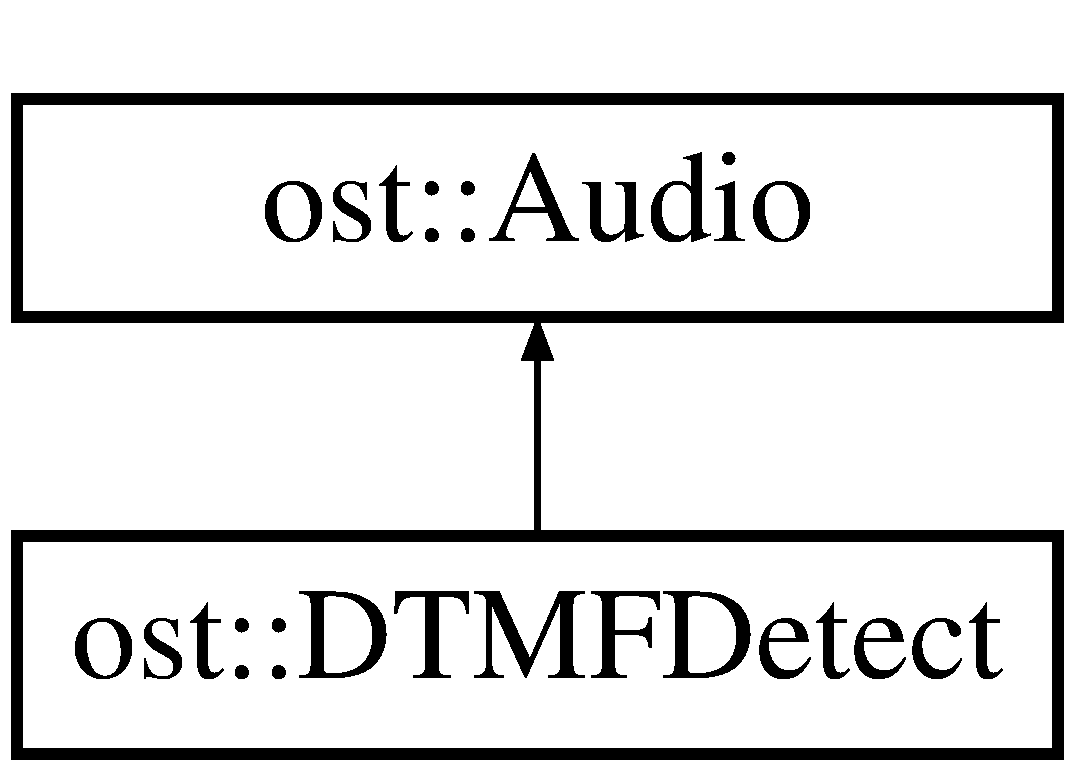
\includegraphics[height=2cm]{classost_1_1_d_t_m_f_detect}
\end{center}
\end{figure}
\subsection*{Public Member Functions}
\begin{DoxyCompactItemize}
\item 
{\bf DTMFDetect} ()
\item 
{\bf $\sim$DTMFDetect} ()
\item 
int {\bf putSamples} ({\bf Linear} buffer, int count)
\begin{DoxyCompactList}\small\item\em This routine is used to push linear audio data into the dtmf tone detection analysizer. \item\end{DoxyCompactList}\item 
int {\bf getResult} (char $\ast$data, int size)
\begin{DoxyCompactList}\small\item\em Copy detected dtmf results into a data buffer. \item\end{DoxyCompactList}\end{DoxyCompactItemize}
\subsection*{Protected Member Functions}
\begin{DoxyCompactItemize}
\item 
void {\bf goertzelInit} ({\bf goertzel\_\-state\_\-t} $\ast$s, tone\_\-detection\_\-descriptor\_\-t $\ast$t)
\item 
void {\bf goertzelUpdate} ({\bf goertzel\_\-state\_\-t} $\ast$s, {\bf Sample} x[$\,$], int samples)
\item 
float {\bf goertzelResult} ({\bf goertzel\_\-state\_\-t} $\ast$s)
\end{DoxyCompactItemize}


\subsection{Detailed Description}
\doxyref{DTMFDetect}{p.}{classost_1_1_d_t_m_f_detect} is used for detecting DTMF tones in a stream of audio. It currently only supports 8000Hz input. 

\subsection{Constructor \& Destructor Documentation}
\index{ost::DTMFDetect@{ost::DTMFDetect}!DTMFDetect@{DTMFDetect}}
\index{DTMFDetect@{DTMFDetect}!ost::DTMFDetect@{ost::DTMFDetect}}
\subsubsection[{DTMFDetect}]{\setlength{\rightskip}{0pt plus 5cm}ost::DTMFDetect::DTMFDetect ()}\label{classost_1_1_d_t_m_f_detect_a9761101bcc763ac4d33c992097482d46}
\index{ost::DTMFDetect@{ost::DTMFDetect}!$\sim$DTMFDetect@{$\sim$DTMFDetect}}
\index{$\sim$DTMFDetect@{$\sim$DTMFDetect}!ost::DTMFDetect@{ost::DTMFDetect}}
\subsubsection[{$\sim$DTMFDetect}]{\setlength{\rightskip}{0pt plus 5cm}ost::DTMFDetect::$\sim$DTMFDetect ()}\label{classost_1_1_d_t_m_f_detect_a1f526ff1431080305aa0ac89601188f2}


\subsection{Member Function Documentation}
\index{ost::DTMFDetect@{ost::DTMFDetect}!getResult@{getResult}}
\index{getResult@{getResult}!ost::DTMFDetect@{ost::DTMFDetect}}
\subsubsection[{getResult}]{\setlength{\rightskip}{0pt plus 5cm}int ost::DTMFDetect::getResult (char $\ast$ {\em data}, \/  int {\em size})}\label{classost_1_1_d_t_m_f_detect_ae33af9f9b942d007b9303810a58be868}


Copy detected dtmf results into a data buffer. 
\begin{DoxyParams}{Parameters}
\item[{\em data}]buffer to copy into. \item[{\em size}]of data buffer to copy into. \end{DoxyParams}
\index{ost::DTMFDetect@{ost::DTMFDetect}!goertzelInit@{goertzelInit}}
\index{goertzelInit@{goertzelInit}!ost::DTMFDetect@{ost::DTMFDetect}}
\subsubsection[{goertzelInit}]{\setlength{\rightskip}{0pt plus 5cm}void ost::DTMFDetect::goertzelInit ({\bf goertzel\_\-state\_\-t} $\ast$ {\em s}, \/  tone\_\-detection\_\-descriptor\_\-t $\ast$ {\em t})\hspace{0.3cm}{\ttfamily  [protected]}}\label{classost_1_1_d_t_m_f_detect_a7613c6d1296fbc51263d6f7e9c50774d}
\index{ost::DTMFDetect@{ost::DTMFDetect}!goertzelResult@{goertzelResult}}
\index{goertzelResult@{goertzelResult}!ost::DTMFDetect@{ost::DTMFDetect}}
\subsubsection[{goertzelResult}]{\setlength{\rightskip}{0pt plus 5cm}float ost::DTMFDetect::goertzelResult ({\bf goertzel\_\-state\_\-t} $\ast$ {\em s})\hspace{0.3cm}{\ttfamily  [protected]}}\label{classost_1_1_d_t_m_f_detect_a225100c6ad08d7f6dcdf9b179bd84bff}
\index{ost::DTMFDetect@{ost::DTMFDetect}!goertzelUpdate@{goertzelUpdate}}
\index{goertzelUpdate@{goertzelUpdate}!ost::DTMFDetect@{ost::DTMFDetect}}
\subsubsection[{goertzelUpdate}]{\setlength{\rightskip}{0pt plus 5cm}void ost::DTMFDetect::goertzelUpdate ({\bf goertzel\_\-state\_\-t} $\ast$ {\em s}, \/  {\bf Sample} {\em x}[$\,$], \/  int {\em samples})\hspace{0.3cm}{\ttfamily  [protected]}}\label{classost_1_1_d_t_m_f_detect_ad6fb18bc0360d281917f8377d88c6871}
\index{ost::DTMFDetect@{ost::DTMFDetect}!putSamples@{putSamples}}
\index{putSamples@{putSamples}!ost::DTMFDetect@{ost::DTMFDetect}}
\subsubsection[{putSamples}]{\setlength{\rightskip}{0pt plus 5cm}int ost::DTMFDetect::putSamples ({\bf Linear} {\em buffer}, \/  int {\em count})}\label{classost_1_1_d_t_m_f_detect_af12fa2c868462ff78e5326a620d98f7a}


This routine is used to push linear audio data into the dtmf tone detection analysizer. It may be called multiple times and results fetched later.


\begin{DoxyParams}{Parameters}
\item[{\em buffer}]of audio data in native machine endian to analysize. \item[{\em count}]of samples to analysize from buffer. \end{DoxyParams}


The documentation for this class was generated from the following file:\begin{DoxyCompactItemize}
\item 
{\bf audio2.h}\end{DoxyCompactItemize}

\section{ost::DTMFTones Class Reference}
\label{classost_1_1_d_t_m_f_tones}\index{ost::DTMFTones@{ost::DTMFTones}}


\doxyref{DTMFTones}{p.}{classost_1_1_d_t_m_f_tones} is used to generate a series of dtmf audio data from a \char`\"{}telephone\char`\"{} number passed as an ASCII string.  


{\ttfamily \#include $<$audio2.h$>$}Inheritance diagram for ost::DTMFTones::\begin{figure}[H]
\begin{center}
\leavevmode
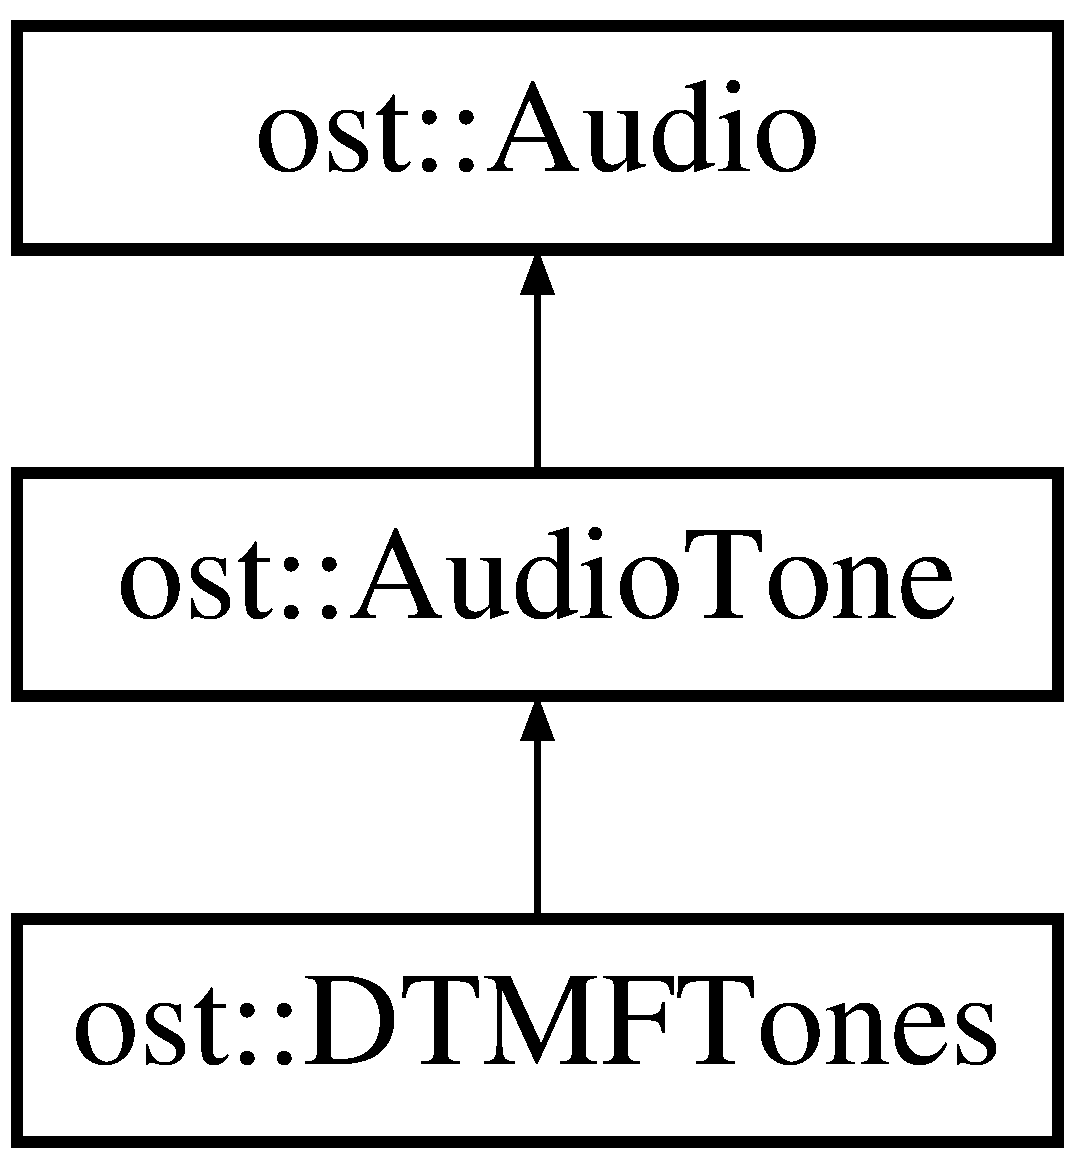
\includegraphics[height=3cm]{classost_1_1_d_t_m_f_tones}
\end{center}
\end{figure}
\subsection*{Public Member Functions}
\begin{DoxyCompactItemize}
\item 
{\bf DTMFTones} (const char $\ast${\bf digits}, {\bf Level} {\bf level}, {\bf timeout\_\-t} duration=20, {\bf timeout\_\-t} interdigit=60)
\begin{DoxyCompactList}\small\item\em Generate a dtmf dialer for a specified dialing string. \item\end{DoxyCompactList}\item 
{\bf $\sim$DTMFTones} ()
\item 
{\bf Linear} {\bf getFrame} (void)
\item 
bool {\bf isComplete} (void)
\end{DoxyCompactItemize}
\subsection*{Protected Attributes}
\begin{DoxyCompactItemize}
\item 
unsigned {\bf remaining}
\item 
unsigned {\bf dtmfframes}
\item 
{\bf timeout\_\-t} {\bf frametime}
\item 
const char $\ast$ {\bf digits}
\item 
{\bf Level} {\bf level}
\item 
bool {\bf complete}
\end{DoxyCompactItemize}


\subsection{Detailed Description}
\doxyref{DTMFTones}{p.}{classost_1_1_d_t_m_f_tones} is used to generate a series of dtmf audio data from a \char`\"{}telephone\char`\"{} number passed as an ASCII string. Each time \doxyref{getFrame()}{p.}{classost_1_1_d_t_m_f_tones_ac59d2ebb1f5feb0aa7871a02109f3b26} is called, the next audio frame of dtmf audio will be created and pulled.

\begin{DoxyAuthor}{Author}
David Sugar $<${\tt dyfet@ostel.com}$>$ Generate DTMF audio 
\end{DoxyAuthor}


\subsection{Constructor \& Destructor Documentation}
\index{ost::DTMFTones@{ost::DTMFTones}!DTMFTones@{DTMFTones}}
\index{DTMFTones@{DTMFTones}!ost::DTMFTones@{ost::DTMFTones}}
\subsubsection[{DTMFTones}]{\setlength{\rightskip}{0pt plus 5cm}ost::DTMFTones::DTMFTones (const char $\ast$ {\em digits}, \/  {\bf Level} {\em level}, \/  {\bf timeout\_\-t} {\em duration} = {\ttfamily 20}, \/  {\bf timeout\_\-t} {\em interdigit} = {\ttfamily 60})}\label{classost_1_1_d_t_m_f_tones_a62570e25d94b2e82f5b384d29107d096}


Generate a dtmf dialer for a specified dialing string. 
\begin{DoxyParams}{Parameters}
\item[{\em digits}]to generate tone dialing for. \item[{\em level}]for dtmf. \item[{\em duration}]timing for generated audio. \item[{\em interdigit}]timing, should be multiple of frame. \end{DoxyParams}
\index{ost::DTMFTones@{ost::DTMFTones}!$\sim$DTMFTones@{$\sim$DTMFTones}}
\index{$\sim$DTMFTones@{$\sim$DTMFTones}!ost::DTMFTones@{ost::DTMFTones}}
\subsubsection[{$\sim$DTMFTones}]{\setlength{\rightskip}{0pt plus 5cm}ost::DTMFTones::$\sim$DTMFTones ()}\label{classost_1_1_d_t_m_f_tones_a8893c69b31f96c7d9aef3daaaf9ca4a9}


\subsection{Member Function Documentation}
\index{ost::DTMFTones@{ost::DTMFTones}!getFrame@{getFrame}}
\index{getFrame@{getFrame}!ost::DTMFTones@{ost::DTMFTones}}
\subsubsection[{getFrame}]{\setlength{\rightskip}{0pt plus 5cm}{\bf Linear} ost::DTMFTones::getFrame (void)\hspace{0.3cm}{\ttfamily  [virtual]}}\label{classost_1_1_d_t_m_f_tones_ac59d2ebb1f5feb0aa7871a02109f3b26}


Reimplemented from {\bf ost::AudioTone} \doxyref{}{p.}{classost_1_1_audio_tone_a943d31930ce0f1318f42d6dc825200cb}.\index{ost::DTMFTones@{ost::DTMFTones}!isComplete@{isComplete}}
\index{isComplete@{isComplete}!ost::DTMFTones@{ost::DTMFTones}}
\subsubsection[{isComplete}]{\setlength{\rightskip}{0pt plus 5cm}bool ost::DTMFTones::isComplete (void)\hspace{0.3cm}{\ttfamily  [virtual]}}\label{classost_1_1_d_t_m_f_tones_a274d70b6b87294764bc50e47f1a8f250}


Reimplemented from {\bf ost::AudioTone} \doxyref{}{p.}{classost_1_1_audio_tone_afd2f4d74c504ff9f1638ac0097f7df8d}.

\subsection{Member Data Documentation}
\index{ost::DTMFTones@{ost::DTMFTones}!complete@{complete}}
\index{complete@{complete}!ost::DTMFTones@{ost::DTMFTones}}
\subsubsection[{complete}]{\setlength{\rightskip}{0pt plus 5cm}bool {\bf ost::DTMFTones::complete}\hspace{0.3cm}{\ttfamily  [protected]}}\label{classost_1_1_d_t_m_f_tones_ad259f2e7159aeda0abc99b1c9e701a74}
\index{ost::DTMFTones@{ost::DTMFTones}!digits@{digits}}
\index{digits@{digits}!ost::DTMFTones@{ost::DTMFTones}}
\subsubsection[{digits}]{\setlength{\rightskip}{0pt plus 5cm}const char$\ast$ {\bf ost::DTMFTones::digits}\hspace{0.3cm}{\ttfamily  [protected]}}\label{classost_1_1_d_t_m_f_tones_a67627cb21e5ff3e615c21e786bd03b8c}
\index{ost::DTMFTones@{ost::DTMFTones}!dtmfframes@{dtmfframes}}
\index{dtmfframes@{dtmfframes}!ost::DTMFTones@{ost::DTMFTones}}
\subsubsection[{dtmfframes}]{\setlength{\rightskip}{0pt plus 5cm}unsigned {\bf ost::DTMFTones::dtmfframes}\hspace{0.3cm}{\ttfamily  [protected]}}\label{classost_1_1_d_t_m_f_tones_ae39e6e3fa09c9b39cee81b7a3123fb10}
\index{ost::DTMFTones@{ost::DTMFTones}!frametime@{frametime}}
\index{frametime@{frametime}!ost::DTMFTones@{ost::DTMFTones}}
\subsubsection[{frametime}]{\setlength{\rightskip}{0pt plus 5cm}{\bf timeout\_\-t} {\bf ost::DTMFTones::frametime}\hspace{0.3cm}{\ttfamily  [protected]}}\label{classost_1_1_d_t_m_f_tones_ab7b645b27130a20d1dd45097f4e1c210}
\index{ost::DTMFTones@{ost::DTMFTones}!level@{level}}
\index{level@{level}!ost::DTMFTones@{ost::DTMFTones}}
\subsubsection[{level}]{\setlength{\rightskip}{0pt plus 5cm}{\bf Level} {\bf ost::DTMFTones::level}\hspace{0.3cm}{\ttfamily  [protected]}}\label{classost_1_1_d_t_m_f_tones_a3b8d23f074e6b74928911a2ffa9546bf}
\index{ost::DTMFTones@{ost::DTMFTones}!remaining@{remaining}}
\index{remaining@{remaining}!ost::DTMFTones@{ost::DTMFTones}}
\subsubsection[{remaining}]{\setlength{\rightskip}{0pt plus 5cm}unsigned {\bf ost::DTMFTones::remaining}\hspace{0.3cm}{\ttfamily  [protected]}}\label{classost_1_1_d_t_m_f_tones_a5177da80d954edb7e140c8cf07a05e75}


The documentation for this class was generated from the following file:\begin{DoxyCompactItemize}
\item 
{\bf audio2.h}\end{DoxyCompactItemize}

\section{ost::Audio::goertzel\_\-state\_\-t Struct Reference}
\label{structost_1_1_audio_1_1goertzel__state__t}\index{ost::Audio::goertzel\_\-state\_\-t@{ost::Audio::goertzel\_\-state\_\-t}}


{\ttfamily \#include $<$audio2.h$>$}\subsection*{Public Attributes}
\begin{DoxyCompactItemize}
\item 
float {\bf v2}
\item 
float {\bf v3}
\item 
float {\bf fac}
\end{DoxyCompactItemize}


\subsection{Member Data Documentation}
\index{ost::Audio::goertzel\_\-state\_\-t@{ost::Audio::goertzel\_\-state\_\-t}!fac@{fac}}
\index{fac@{fac}!ost::Audio::goertzel_state_t@{ost::Audio::goertzel\_\-state\_\-t}}
\subsubsection[{fac}]{\setlength{\rightskip}{0pt plus 5cm}float {\bf ost::Audio::goertzel\_\-state\_\-t::fac}}\label{structost_1_1_audio_1_1goertzel__state__t_a1630fc16b30ad926fb0ea8d1b63716a5}
\index{ost::Audio::goertzel\_\-state\_\-t@{ost::Audio::goertzel\_\-state\_\-t}!v2@{v2}}
\index{v2@{v2}!ost::Audio::goertzel_state_t@{ost::Audio::goertzel\_\-state\_\-t}}
\subsubsection[{v2}]{\setlength{\rightskip}{0pt plus 5cm}float {\bf ost::Audio::goertzel\_\-state\_\-t::v2}}\label{structost_1_1_audio_1_1goertzel__state__t_a1a7405840dfec270e33a47cabcdff91f}
\index{ost::Audio::goertzel\_\-state\_\-t@{ost::Audio::goertzel\_\-state\_\-t}!v3@{v3}}
\index{v3@{v3}!ost::Audio::goertzel_state_t@{ost::Audio::goertzel\_\-state\_\-t}}
\subsubsection[{v3}]{\setlength{\rightskip}{0pt plus 5cm}float {\bf ost::Audio::goertzel\_\-state\_\-t::v3}}\label{structost_1_1_audio_1_1goertzel__state__t_ab100a79a96a5baeeb2792adf9e5401b0}


The documentation for this struct was generated from the following file:\begin{DoxyCompactItemize}
\item 
{\bf audio2.h}\end{DoxyCompactItemize}

\section{ost::Audio::Info Class Reference}
\label{classost_1_1_audio_1_1_info}\index{ost::Audio::Info@{ost::Audio::Info}}


\doxyref{Audio}{p.}{classost_1_1_audio} source description.  


{\ttfamily \#include $<$audio2.h$>$}\subsection*{Public Member Functions}
\begin{DoxyCompactItemize}
\item 
{\bf Info} ()
\item 
void {\bf clear} (void)
\item 
void {\bf set} (void)
\item 
void {\bf setFraming} ({\bf timeout\_\-t} frame)
\item 
void {\bf setRate} ({\bf Rate} {\bf rate})
\end{DoxyCompactItemize}
\subsection*{Public Attributes}
\begin{DoxyCompactItemize}
\item 
{\bf Format} {\bf format}
\item 
{\bf Encoding} {\bf encoding}
\item 
unsigned long {\bf rate}
\item 
unsigned long {\bf bitrate}
\item 
unsigned {\bf order}
\item 
unsigned {\bf framesize}
\item 
unsigned {\bf framecount}
\item 
unsigned {\bf headersize}
\item 
unsigned {\bf padding}
\item 
{\bf timeout\_\-t} {\bf framing}
\item 
char $\ast$ {\bf annotation}
\end{DoxyCompactItemize}


\subsection{Detailed Description}
\doxyref{Audio}{p.}{classost_1_1_audio} source description. 

\subsection{Constructor \& Destructor Documentation}
\index{ost::Audio::Info@{ost::Audio::Info}!Info@{Info}}
\index{Info@{Info}!ost::Audio::Info@{ost::Audio::Info}}
\subsubsection[{Info}]{\setlength{\rightskip}{0pt plus 5cm}ost::Audio::Info::Info ()}\label{classost_1_1_audio_1_1_info_a08bd364745a62238514c6591a950a9ab}


\subsection{Member Function Documentation}
\index{ost::Audio::Info@{ost::Audio::Info}!clear@{clear}}
\index{clear@{clear}!ost::Audio::Info@{ost::Audio::Info}}
\subsubsection[{clear}]{\setlength{\rightskip}{0pt plus 5cm}void ost::Audio::Info::clear (void)}\label{classost_1_1_audio_1_1_info_af68c40e779091f736c8782e35ac611a6}
\index{ost::Audio::Info@{ost::Audio::Info}!set@{set}}
\index{set@{set}!ost::Audio::Info@{ost::Audio::Info}}
\subsubsection[{set}]{\setlength{\rightskip}{0pt plus 5cm}void ost::Audio::Info::set (void)}\label{classost_1_1_audio_1_1_info_a4630246844b6994828766d8a30a906d2}
\index{ost::Audio::Info@{ost::Audio::Info}!setFraming@{setFraming}}
\index{setFraming@{setFraming}!ost::Audio::Info@{ost::Audio::Info}}
\subsubsection[{setFraming}]{\setlength{\rightskip}{0pt plus 5cm}void ost::Audio::Info::setFraming ({\bf timeout\_\-t} {\em frame})}\label{classost_1_1_audio_1_1_info_aeda8145d804ae0c950ab43fb929a10ea}
\index{ost::Audio::Info@{ost::Audio::Info}!setRate@{setRate}}
\index{setRate@{setRate}!ost::Audio::Info@{ost::Audio::Info}}
\subsubsection[{setRate}]{\setlength{\rightskip}{0pt plus 5cm}void ost::Audio::Info::setRate ({\bf Rate} {\em rate})}\label{classost_1_1_audio_1_1_info_ad760deec6ae467c9daadcd452547835c}


\subsection{Member Data Documentation}
\index{ost::Audio::Info@{ost::Audio::Info}!annotation@{annotation}}
\index{annotation@{annotation}!ost::Audio::Info@{ost::Audio::Info}}
\subsubsection[{annotation}]{\setlength{\rightskip}{0pt plus 5cm}char$\ast$ {\bf ost::Audio::Info::annotation}}\label{classost_1_1_audio_1_1_info_a84f470ef63154d5b8c040e850a89dcb4}
\index{ost::Audio::Info@{ost::Audio::Info}!bitrate@{bitrate}}
\index{bitrate@{bitrate}!ost::Audio::Info@{ost::Audio::Info}}
\subsubsection[{bitrate}]{\setlength{\rightskip}{0pt plus 5cm}unsigned long {\bf ost::Audio::Info::bitrate}}\label{classost_1_1_audio_1_1_info_a7f3155677b7414ec2b00138a9252b980}
\index{ost::Audio::Info@{ost::Audio::Info}!encoding@{encoding}}
\index{encoding@{encoding}!ost::Audio::Info@{ost::Audio::Info}}
\subsubsection[{encoding}]{\setlength{\rightskip}{0pt plus 5cm}{\bf Encoding} {\bf ost::Audio::Info::encoding}}\label{classost_1_1_audio_1_1_info_a247ab7f4d83b8b160c3d6e61fbc534d7}
\index{ost::Audio::Info@{ost::Audio::Info}!format@{format}}
\index{format@{format}!ost::Audio::Info@{ost::Audio::Info}}
\subsubsection[{format}]{\setlength{\rightskip}{0pt plus 5cm}{\bf Format} {\bf ost::Audio::Info::format}}\label{classost_1_1_audio_1_1_info_ad6a3424809c431bed4dcbe008d6e7fe4}
\index{ost::Audio::Info@{ost::Audio::Info}!framecount@{framecount}}
\index{framecount@{framecount}!ost::Audio::Info@{ost::Audio::Info}}
\subsubsection[{framecount}]{\setlength{\rightskip}{0pt plus 5cm}unsigned {\bf ost::Audio::Info::framecount}}\label{classost_1_1_audio_1_1_info_ad9a8665590be0f4ea174fb87ed591f48}
\index{ost::Audio::Info@{ost::Audio::Info}!framesize@{framesize}}
\index{framesize@{framesize}!ost::Audio::Info@{ost::Audio::Info}}
\subsubsection[{framesize}]{\setlength{\rightskip}{0pt plus 5cm}unsigned {\bf ost::Audio::Info::framesize}}\label{classost_1_1_audio_1_1_info_a6f88389b27d7d57c42a6fe22b924f809}
\index{ost::Audio::Info@{ost::Audio::Info}!framing@{framing}}
\index{framing@{framing}!ost::Audio::Info@{ost::Audio::Info}}
\subsubsection[{framing}]{\setlength{\rightskip}{0pt plus 5cm}{\bf timeout\_\-t} {\bf ost::Audio::Info::framing}}\label{classost_1_1_audio_1_1_info_a562f918a4f1d73d605a2eb49eb6c4786}
\index{ost::Audio::Info@{ost::Audio::Info}!headersize@{headersize}}
\index{headersize@{headersize}!ost::Audio::Info@{ost::Audio::Info}}
\subsubsection[{headersize}]{\setlength{\rightskip}{0pt plus 5cm}unsigned {\bf ost::Audio::Info::headersize}}\label{classost_1_1_audio_1_1_info_a8fa6cac96df3c014db58370e5e46d530}
\index{ost::Audio::Info@{ost::Audio::Info}!order@{order}}
\index{order@{order}!ost::Audio::Info@{ost::Audio::Info}}
\subsubsection[{order}]{\setlength{\rightskip}{0pt plus 5cm}unsigned {\bf ost::Audio::Info::order}}\label{classost_1_1_audio_1_1_info_a48a648aaef83abb6fd65fc59dcf40467}
\index{ost::Audio::Info@{ost::Audio::Info}!padding@{padding}}
\index{padding@{padding}!ost::Audio::Info@{ost::Audio::Info}}
\subsubsection[{padding}]{\setlength{\rightskip}{0pt plus 5cm}unsigned {\bf ost::Audio::Info::padding}}\label{classost_1_1_audio_1_1_info_a62bc343ffa9bef02d98af2168976615a}
\index{ost::Audio::Info@{ost::Audio::Info}!rate@{rate}}
\index{rate@{rate}!ost::Audio::Info@{ost::Audio::Info}}
\subsubsection[{rate}]{\setlength{\rightskip}{0pt plus 5cm}unsigned long {\bf ost::Audio::Info::rate}}\label{classost_1_1_audio_1_1_info_aa2da9a01f49ef6c0d191580ab7235ceb}


The documentation for this class was generated from the following file:\begin{DoxyCompactItemize}
\item 
{\bf audio2.h}\end{DoxyCompactItemize}

\section{ost::MFTones Class Reference}
\label{classost_1_1_m_f_tones}\index{ost::MFTones@{ost::MFTones}}


\doxyref{MFTones}{p.}{classost_1_1_m_f_tones} is used to generate a series of mf audio data from a \char`\"{}telephone\char`\"{} number passed as an ASCII string.  


{\ttfamily \#include $<$audio2.h$>$}Inheritance diagram for ost::MFTones::\begin{figure}[H]
\begin{center}
\leavevmode
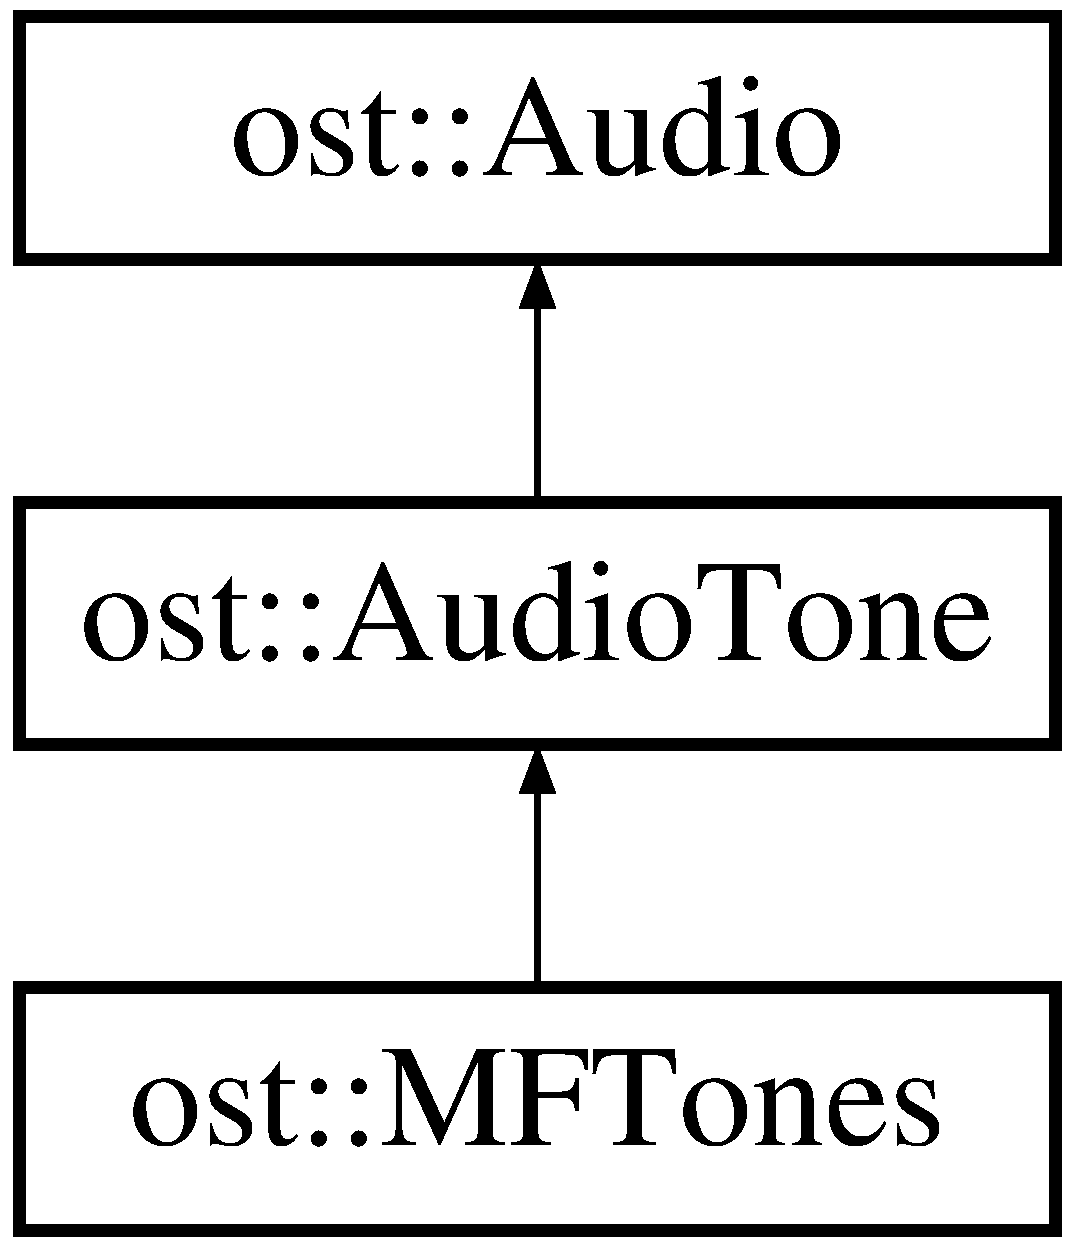
\includegraphics[height=3cm]{classost_1_1_m_f_tones}
\end{center}
\end{figure}
\subsection*{Public Member Functions}
\begin{DoxyCompactItemize}
\item 
{\bf MFTones} (const char $\ast${\bf digits}, {\bf Level} {\bf level}, {\bf timeout\_\-t} duration=20, {\bf timeout\_\-t} interdigit=60)
\begin{DoxyCompactList}\small\item\em Generate a mf dialer for a specified dialing string. \item\end{DoxyCompactList}\item 
{\bf $\sim$MFTones} ()
\item 
{\bf Linear} {\bf getFrame} (void)
\item 
bool {\bf isComplete} (void)
\end{DoxyCompactItemize}
\subsection*{Protected Attributes}
\begin{DoxyCompactItemize}
\item 
unsigned {\bf remaining}
\item 
unsigned {\bf mfframes}
\item 
{\bf timeout\_\-t} {\bf frametime}
\item 
const char $\ast$ {\bf digits}
\item 
{\bf Level} {\bf level}
\item 
bool {\bf complete}
\item 
bool {\bf kflag}
\end{DoxyCompactItemize}


\subsection{Detailed Description}
\doxyref{MFTones}{p.}{classost_1_1_m_f_tones} is used to generate a series of mf audio data from a \char`\"{}telephone\char`\"{} number passed as an ASCII string. Each time \doxyref{getFrame()}{p.}{classost_1_1_m_f_tones_a1e3cb8bbbbe783bc7f4f40a2162ad713} is called, the next audio frame of dtmf audio will be created and pulled.

\begin{DoxyAuthor}{Author}
David Sugar $<${\tt dyfet@ostel.com}$>$ Generate MF audio 
\end{DoxyAuthor}


\subsection{Constructor \& Destructor Documentation}
\index{ost::MFTones@{ost::MFTones}!MFTones@{MFTones}}
\index{MFTones@{MFTones}!ost::MFTones@{ost::MFTones}}
\subsubsection[{MFTones}]{\setlength{\rightskip}{0pt plus 5cm}ost::MFTones::MFTones (const char $\ast$ {\em digits}, \/  {\bf Level} {\em level}, \/  {\bf timeout\_\-t} {\em duration} = {\ttfamily 20}, \/  {\bf timeout\_\-t} {\em interdigit} = {\ttfamily 60})}\label{classost_1_1_m_f_tones_ae9d48c4d9de53b7e1b861548c8c07b38}


Generate a mf dialer for a specified dialing string. 
\begin{DoxyParams}{Parameters}
\item[{\em digits}]to generate tone dialing for. \item[{\em level}]for mf. \item[{\em duration}]timing for generated audio. \item[{\em interdigit}]timing, should be multiple of frame. \end{DoxyParams}
\index{ost::MFTones@{ost::MFTones}!$\sim$MFTones@{$\sim$MFTones}}
\index{$\sim$MFTones@{$\sim$MFTones}!ost::MFTones@{ost::MFTones}}
\subsubsection[{$\sim$MFTones}]{\setlength{\rightskip}{0pt plus 5cm}ost::MFTones::$\sim$MFTones ()}\label{classost_1_1_m_f_tones_a43b51accde7cd36306565325a44895bc}


\subsection{Member Function Documentation}
\index{ost::MFTones@{ost::MFTones}!getFrame@{getFrame}}
\index{getFrame@{getFrame}!ost::MFTones@{ost::MFTones}}
\subsubsection[{getFrame}]{\setlength{\rightskip}{0pt plus 5cm}{\bf Linear} ost::MFTones::getFrame (void)\hspace{0.3cm}{\ttfamily  [virtual]}}\label{classost_1_1_m_f_tones_a1e3cb8bbbbe783bc7f4f40a2162ad713}


Reimplemented from {\bf ost::AudioTone} \doxyref{}{p.}{classost_1_1_audio_tone_a943d31930ce0f1318f42d6dc825200cb}.\index{ost::MFTones@{ost::MFTones}!isComplete@{isComplete}}
\index{isComplete@{isComplete}!ost::MFTones@{ost::MFTones}}
\subsubsection[{isComplete}]{\setlength{\rightskip}{0pt plus 5cm}bool ost::MFTones::isComplete (void)\hspace{0.3cm}{\ttfamily  [virtual]}}\label{classost_1_1_m_f_tones_a1a889d81dba1bdbc01d55c25d0b348b1}


Reimplemented from {\bf ost::AudioTone} \doxyref{}{p.}{classost_1_1_audio_tone_afd2f4d74c504ff9f1638ac0097f7df8d}.

\subsection{Member Data Documentation}
\index{ost::MFTones@{ost::MFTones}!complete@{complete}}
\index{complete@{complete}!ost::MFTones@{ost::MFTones}}
\subsubsection[{complete}]{\setlength{\rightskip}{0pt plus 5cm}bool {\bf ost::MFTones::complete}\hspace{0.3cm}{\ttfamily  [protected]}}\label{classost_1_1_m_f_tones_a454e89ef50ff60437542c3aa9eb6dd32}
\index{ost::MFTones@{ost::MFTones}!digits@{digits}}
\index{digits@{digits}!ost::MFTones@{ost::MFTones}}
\subsubsection[{digits}]{\setlength{\rightskip}{0pt plus 5cm}const char$\ast$ {\bf ost::MFTones::digits}\hspace{0.3cm}{\ttfamily  [protected]}}\label{classost_1_1_m_f_tones_a7040ba98563c1c07b1b259db2c70f7b6}
\index{ost::MFTones@{ost::MFTones}!frametime@{frametime}}
\index{frametime@{frametime}!ost::MFTones@{ost::MFTones}}
\subsubsection[{frametime}]{\setlength{\rightskip}{0pt plus 5cm}{\bf timeout\_\-t} {\bf ost::MFTones::frametime}\hspace{0.3cm}{\ttfamily  [protected]}}\label{classost_1_1_m_f_tones_a1ab0b75fcd4a6c2b6307293f418536cc}
\index{ost::MFTones@{ost::MFTones}!kflag@{kflag}}
\index{kflag@{kflag}!ost::MFTones@{ost::MFTones}}
\subsubsection[{kflag}]{\setlength{\rightskip}{0pt plus 5cm}bool {\bf ost::MFTones::kflag}\hspace{0.3cm}{\ttfamily  [protected]}}\label{classost_1_1_m_f_tones_aa7f10829db96089ad0078a07b55621c6}
\index{ost::MFTones@{ost::MFTones}!level@{level}}
\index{level@{level}!ost::MFTones@{ost::MFTones}}
\subsubsection[{level}]{\setlength{\rightskip}{0pt plus 5cm}{\bf Level} {\bf ost::MFTones::level}\hspace{0.3cm}{\ttfamily  [protected]}}\label{classost_1_1_m_f_tones_aa2dbf77e15507a7b7c14d3b66d7c991e}
\index{ost::MFTones@{ost::MFTones}!mfframes@{mfframes}}
\index{mfframes@{mfframes}!ost::MFTones@{ost::MFTones}}
\subsubsection[{mfframes}]{\setlength{\rightskip}{0pt plus 5cm}unsigned {\bf ost::MFTones::mfframes}\hspace{0.3cm}{\ttfamily  [protected]}}\label{classost_1_1_m_f_tones_abc6f3c983a816cf8a69b25ed90eb65cc}
\index{ost::MFTones@{ost::MFTones}!remaining@{remaining}}
\index{remaining@{remaining}!ost::MFTones@{ost::MFTones}}
\subsubsection[{remaining}]{\setlength{\rightskip}{0pt plus 5cm}unsigned {\bf ost::MFTones::remaining}\hspace{0.3cm}{\ttfamily  [protected]}}\label{classost_1_1_m_f_tones_a9057503a5760fb278c0a461d9b786043}


The documentation for this class was generated from the following file:\begin{DoxyCompactItemize}
\item 
{\bf audio2.h}\end{DoxyCompactItemize}

\section{ost::Audio::mpeg\_\-audio Struct Reference}
\label{structost_1_1_audio_1_1mpeg__audio}\index{ost::Audio::mpeg\_\-audio@{ost::Audio::mpeg\_\-audio}}


{\ttfamily \#include $<$audio2.h$>$}\subsection*{Public Attributes}
\begin{DoxyCompactItemize}
\item 
unsigned char {\bf mp\_\-sync1}: 8
\item 
unsigned char {\bf mp\_\-crc}: 1
\item 
unsigned char {\bf mp\_\-layer}: 2
\item 
unsigned char {\bf mp\_\-ver}: 2
\item 
unsigned char {\bf mp\_\-sync2}: 3
\item 
unsigned char {\bf mp\_\-priv}: 1
\item 
unsigned char {\bf mp\_\-pad}: 1
\item 
unsigned char {\bf mp\_\-srate}: 2
\item 
unsigned char {\bf mp\_\-brate}: 4
\item 
unsigned char {\bf mp\_\-emp}: 2
\item 
unsigned char {\bf mp\_\-original}: 1
\item 
unsigned char {\bf mp\_\-copyright}: 1
\item 
unsigned char {\bf mp\_\-extend}: 2
\item 
unsigned char {\bf mp\_\-channels}: 2
\end{DoxyCompactItemize}


\subsection{Member Data Documentation}
\index{ost::Audio::mpeg\_\-audio@{ost::Audio::mpeg\_\-audio}!mp\_\-brate@{mp\_\-brate}}
\index{mp\_\-brate@{mp\_\-brate}!ost::Audio::mpeg_audio@{ost::Audio::mpeg\_\-audio}}
\subsubsection[{mp\_\-brate}]{\setlength{\rightskip}{0pt plus 5cm}unsigned char {\bf ost::Audio::mpeg\_\-audio::mp\_\-brate}}\label{structost_1_1_audio_1_1mpeg__audio_ab9679401bb55fbaa2121ab3f81d4a7ea}
\index{ost::Audio::mpeg\_\-audio@{ost::Audio::mpeg\_\-audio}!mp\_\-channels@{mp\_\-channels}}
\index{mp\_\-channels@{mp\_\-channels}!ost::Audio::mpeg_audio@{ost::Audio::mpeg\_\-audio}}
\subsubsection[{mp\_\-channels}]{\setlength{\rightskip}{0pt plus 5cm}unsigned char {\bf ost::Audio::mpeg\_\-audio::mp\_\-channels}}\label{structost_1_1_audio_1_1mpeg__audio_a1eb170358a872fd480c55a28ce5c5f4e}
\index{ost::Audio::mpeg\_\-audio@{ost::Audio::mpeg\_\-audio}!mp\_\-copyright@{mp\_\-copyright}}
\index{mp\_\-copyright@{mp\_\-copyright}!ost::Audio::mpeg_audio@{ost::Audio::mpeg\_\-audio}}
\subsubsection[{mp\_\-copyright}]{\setlength{\rightskip}{0pt plus 5cm}unsigned char {\bf ost::Audio::mpeg\_\-audio::mp\_\-copyright}}\label{structost_1_1_audio_1_1mpeg__audio_acb81e5190c07f6d22575b4f1a17cdead}
\index{ost::Audio::mpeg\_\-audio@{ost::Audio::mpeg\_\-audio}!mp\_\-crc@{mp\_\-crc}}
\index{mp\_\-crc@{mp\_\-crc}!ost::Audio::mpeg_audio@{ost::Audio::mpeg\_\-audio}}
\subsubsection[{mp\_\-crc}]{\setlength{\rightskip}{0pt plus 5cm}unsigned char {\bf ost::Audio::mpeg\_\-audio::mp\_\-crc}}\label{structost_1_1_audio_1_1mpeg__audio_a8b3a4d39a2cf71c8ed19f58c734bb028}
\index{ost::Audio::mpeg\_\-audio@{ost::Audio::mpeg\_\-audio}!mp\_\-emp@{mp\_\-emp}}
\index{mp\_\-emp@{mp\_\-emp}!ost::Audio::mpeg_audio@{ost::Audio::mpeg\_\-audio}}
\subsubsection[{mp\_\-emp}]{\setlength{\rightskip}{0pt plus 5cm}unsigned char {\bf ost::Audio::mpeg\_\-audio::mp\_\-emp}}\label{structost_1_1_audio_1_1mpeg__audio_a392dcd9969ac7cb5593d5ace9d4ba409}
\index{ost::Audio::mpeg\_\-audio@{ost::Audio::mpeg\_\-audio}!mp\_\-extend@{mp\_\-extend}}
\index{mp\_\-extend@{mp\_\-extend}!ost::Audio::mpeg_audio@{ost::Audio::mpeg\_\-audio}}
\subsubsection[{mp\_\-extend}]{\setlength{\rightskip}{0pt plus 5cm}unsigned char {\bf ost::Audio::mpeg\_\-audio::mp\_\-extend}}\label{structost_1_1_audio_1_1mpeg__audio_a1421a91dc9134069505db80b6a16774b}
\index{ost::Audio::mpeg\_\-audio@{ost::Audio::mpeg\_\-audio}!mp\_\-layer@{mp\_\-layer}}
\index{mp\_\-layer@{mp\_\-layer}!ost::Audio::mpeg_audio@{ost::Audio::mpeg\_\-audio}}
\subsubsection[{mp\_\-layer}]{\setlength{\rightskip}{0pt plus 5cm}unsigned char {\bf ost::Audio::mpeg\_\-audio::mp\_\-layer}}\label{structost_1_1_audio_1_1mpeg__audio_a2cddde96a4560692692a273faa5fca9b}
\index{ost::Audio::mpeg\_\-audio@{ost::Audio::mpeg\_\-audio}!mp\_\-original@{mp\_\-original}}
\index{mp\_\-original@{mp\_\-original}!ost::Audio::mpeg_audio@{ost::Audio::mpeg\_\-audio}}
\subsubsection[{mp\_\-original}]{\setlength{\rightskip}{0pt plus 5cm}unsigned char {\bf ost::Audio::mpeg\_\-audio::mp\_\-original}}\label{structost_1_1_audio_1_1mpeg__audio_a9c0e0afae7ade43bdcf638fbbfe3064f}
\index{ost::Audio::mpeg\_\-audio@{ost::Audio::mpeg\_\-audio}!mp\_\-pad@{mp\_\-pad}}
\index{mp\_\-pad@{mp\_\-pad}!ost::Audio::mpeg_audio@{ost::Audio::mpeg\_\-audio}}
\subsubsection[{mp\_\-pad}]{\setlength{\rightskip}{0pt plus 5cm}unsigned char {\bf ost::Audio::mpeg\_\-audio::mp\_\-pad}}\label{structost_1_1_audio_1_1mpeg__audio_adb85e53fff084c4cf8d9e80d6c57f2a3}
\index{ost::Audio::mpeg\_\-audio@{ost::Audio::mpeg\_\-audio}!mp\_\-priv@{mp\_\-priv}}
\index{mp\_\-priv@{mp\_\-priv}!ost::Audio::mpeg_audio@{ost::Audio::mpeg\_\-audio}}
\subsubsection[{mp\_\-priv}]{\setlength{\rightskip}{0pt plus 5cm}unsigned char {\bf ost::Audio::mpeg\_\-audio::mp\_\-priv}}\label{structost_1_1_audio_1_1mpeg__audio_a056edee325af640d28b9ec1761a8d1ff}
\index{ost::Audio::mpeg\_\-audio@{ost::Audio::mpeg\_\-audio}!mp\_\-srate@{mp\_\-srate}}
\index{mp\_\-srate@{mp\_\-srate}!ost::Audio::mpeg_audio@{ost::Audio::mpeg\_\-audio}}
\subsubsection[{mp\_\-srate}]{\setlength{\rightskip}{0pt plus 5cm}unsigned char {\bf ost::Audio::mpeg\_\-audio::mp\_\-srate}}\label{structost_1_1_audio_1_1mpeg__audio_a45345a1a20d3e274bd02c3079e7a04c1}
\index{ost::Audio::mpeg\_\-audio@{ost::Audio::mpeg\_\-audio}!mp\_\-sync1@{mp\_\-sync1}}
\index{mp\_\-sync1@{mp\_\-sync1}!ost::Audio::mpeg_audio@{ost::Audio::mpeg\_\-audio}}
\subsubsection[{mp\_\-sync1}]{\setlength{\rightskip}{0pt plus 5cm}unsigned char {\bf ost::Audio::mpeg\_\-audio::mp\_\-sync1}}\label{structost_1_1_audio_1_1mpeg__audio_a0616c2cf1ca66cc7d4e6e723cd1a1a8c}
\index{ost::Audio::mpeg\_\-audio@{ost::Audio::mpeg\_\-audio}!mp\_\-sync2@{mp\_\-sync2}}
\index{mp\_\-sync2@{mp\_\-sync2}!ost::Audio::mpeg_audio@{ost::Audio::mpeg\_\-audio}}
\subsubsection[{mp\_\-sync2}]{\setlength{\rightskip}{0pt plus 5cm}unsigned char {\bf ost::Audio::mpeg\_\-audio::mp\_\-sync2}}\label{structost_1_1_audio_1_1mpeg__audio_a912522e501564727926bda6fa1751bb4}
\index{ost::Audio::mpeg\_\-audio@{ost::Audio::mpeg\_\-audio}!mp\_\-ver@{mp\_\-ver}}
\index{mp\_\-ver@{mp\_\-ver}!ost::Audio::mpeg_audio@{ost::Audio::mpeg\_\-audio}}
\subsubsection[{mp\_\-ver}]{\setlength{\rightskip}{0pt plus 5cm}unsigned char {\bf ost::Audio::mpeg\_\-audio::mp\_\-ver}}\label{structost_1_1_audio_1_1mpeg__audio_a33787fdb19fef66e02011746cb6a258a}


The documentation for this struct was generated from the following file:\begin{DoxyCompactItemize}
\item 
{\bf audio2.h}\end{DoxyCompactItemize}

\section{ost::Audio::mpeg\_\-tagv1 Struct Reference}
\label{structost_1_1_audio_1_1mpeg__tagv1}\index{ost::Audio::mpeg\_\-tagv1@{ost::Audio::mpeg\_\-tagv1}}


{\ttfamily \#include $<$audio2.h$>$}\subsection*{Public Attributes}
\begin{DoxyCompactItemize}
\item 
char {\bf tag\_\-id} [3]
\item 
char {\bf tag\_\-title} [30]
\item 
char {\bf tag\_\-artist} [30]
\item 
char {\bf tag\_\-album} [30]
\item 
char {\bf tag\_\-year} [4]
\item 
char {\bf tag\_\-note} [30]
\item 
unsigned char {\bf genre}
\end{DoxyCompactItemize}


\subsection{Member Data Documentation}
\index{ost::Audio::mpeg\_\-tagv1@{ost::Audio::mpeg\_\-tagv1}!genre@{genre}}
\index{genre@{genre}!ost::Audio::mpeg_tagv1@{ost::Audio::mpeg\_\-tagv1}}
\subsubsection[{genre}]{\setlength{\rightskip}{0pt plus 5cm}unsigned char {\bf ost::Audio::mpeg\_\-tagv1::genre}}\label{structost_1_1_audio_1_1mpeg__tagv1_a0e19702524085e531f8cf9d8e227598c}
\index{ost::Audio::mpeg\_\-tagv1@{ost::Audio::mpeg\_\-tagv1}!tag\_\-album@{tag\_\-album}}
\index{tag\_\-album@{tag\_\-album}!ost::Audio::mpeg_tagv1@{ost::Audio::mpeg\_\-tagv1}}
\subsubsection[{tag\_\-album}]{\setlength{\rightskip}{0pt plus 5cm}char {\bf ost::Audio::mpeg\_\-tagv1::tag\_\-album}[30]}\label{structost_1_1_audio_1_1mpeg__tagv1_a3d2dc3ef39cd5cf32ed00c88719a5b08}
\index{ost::Audio::mpeg\_\-tagv1@{ost::Audio::mpeg\_\-tagv1}!tag\_\-artist@{tag\_\-artist}}
\index{tag\_\-artist@{tag\_\-artist}!ost::Audio::mpeg_tagv1@{ost::Audio::mpeg\_\-tagv1}}
\subsubsection[{tag\_\-artist}]{\setlength{\rightskip}{0pt plus 5cm}char {\bf ost::Audio::mpeg\_\-tagv1::tag\_\-artist}[30]}\label{structost_1_1_audio_1_1mpeg__tagv1_aaec2a7c165378db68d95840e63640e4c}
\index{ost::Audio::mpeg\_\-tagv1@{ost::Audio::mpeg\_\-tagv1}!tag\_\-id@{tag\_\-id}}
\index{tag\_\-id@{tag\_\-id}!ost::Audio::mpeg_tagv1@{ost::Audio::mpeg\_\-tagv1}}
\subsubsection[{tag\_\-id}]{\setlength{\rightskip}{0pt plus 5cm}char {\bf ost::Audio::mpeg\_\-tagv1::tag\_\-id}[3]}\label{structost_1_1_audio_1_1mpeg__tagv1_ae9fe8188284d7aa1307570dac5e46475}
\index{ost::Audio::mpeg\_\-tagv1@{ost::Audio::mpeg\_\-tagv1}!tag\_\-note@{tag\_\-note}}
\index{tag\_\-note@{tag\_\-note}!ost::Audio::mpeg_tagv1@{ost::Audio::mpeg\_\-tagv1}}
\subsubsection[{tag\_\-note}]{\setlength{\rightskip}{0pt plus 5cm}char {\bf ost::Audio::mpeg\_\-tagv1::tag\_\-note}[30]}\label{structost_1_1_audio_1_1mpeg__tagv1_ad5f2e78c6836abb8231b35dd709c4bba}
\index{ost::Audio::mpeg\_\-tagv1@{ost::Audio::mpeg\_\-tagv1}!tag\_\-title@{tag\_\-title}}
\index{tag\_\-title@{tag\_\-title}!ost::Audio::mpeg_tagv1@{ost::Audio::mpeg\_\-tagv1}}
\subsubsection[{tag\_\-title}]{\setlength{\rightskip}{0pt plus 5cm}char {\bf ost::Audio::mpeg\_\-tagv1::tag\_\-title}[30]}\label{structost_1_1_audio_1_1mpeg__tagv1_adfa7e43219245b81587495f2b8b13c4c}
\index{ost::Audio::mpeg\_\-tagv1@{ost::Audio::mpeg\_\-tagv1}!tag\_\-year@{tag\_\-year}}
\index{tag\_\-year@{tag\_\-year}!ost::Audio::mpeg_tagv1@{ost::Audio::mpeg\_\-tagv1}}
\subsubsection[{tag\_\-year}]{\setlength{\rightskip}{0pt plus 5cm}char {\bf ost::Audio::mpeg\_\-tagv1::tag\_\-year}[4]}\label{structost_1_1_audio_1_1mpeg__tagv1_a8fa333a7e97cf9b4e4750b47fc86f6d7}


The documentation for this struct was generated from the following file:\begin{DoxyCompactItemize}
\item 
{\bf audio2.h}\end{DoxyCompactItemize}

\section{ost::TelTone Class Reference}
\label{classost_1_1_tel_tone}\index{ost::TelTone@{ost::TelTone}}


An object that is used to sequence and extract telephony tones based on a telephony tone descriptor retrieved from the parsed international telephony tone database.  


{\ttfamily \#include $<$audio2.h$>$}Inheritance diagram for ost::TelTone::\begin{figure}[H]
\begin{center}
\leavevmode
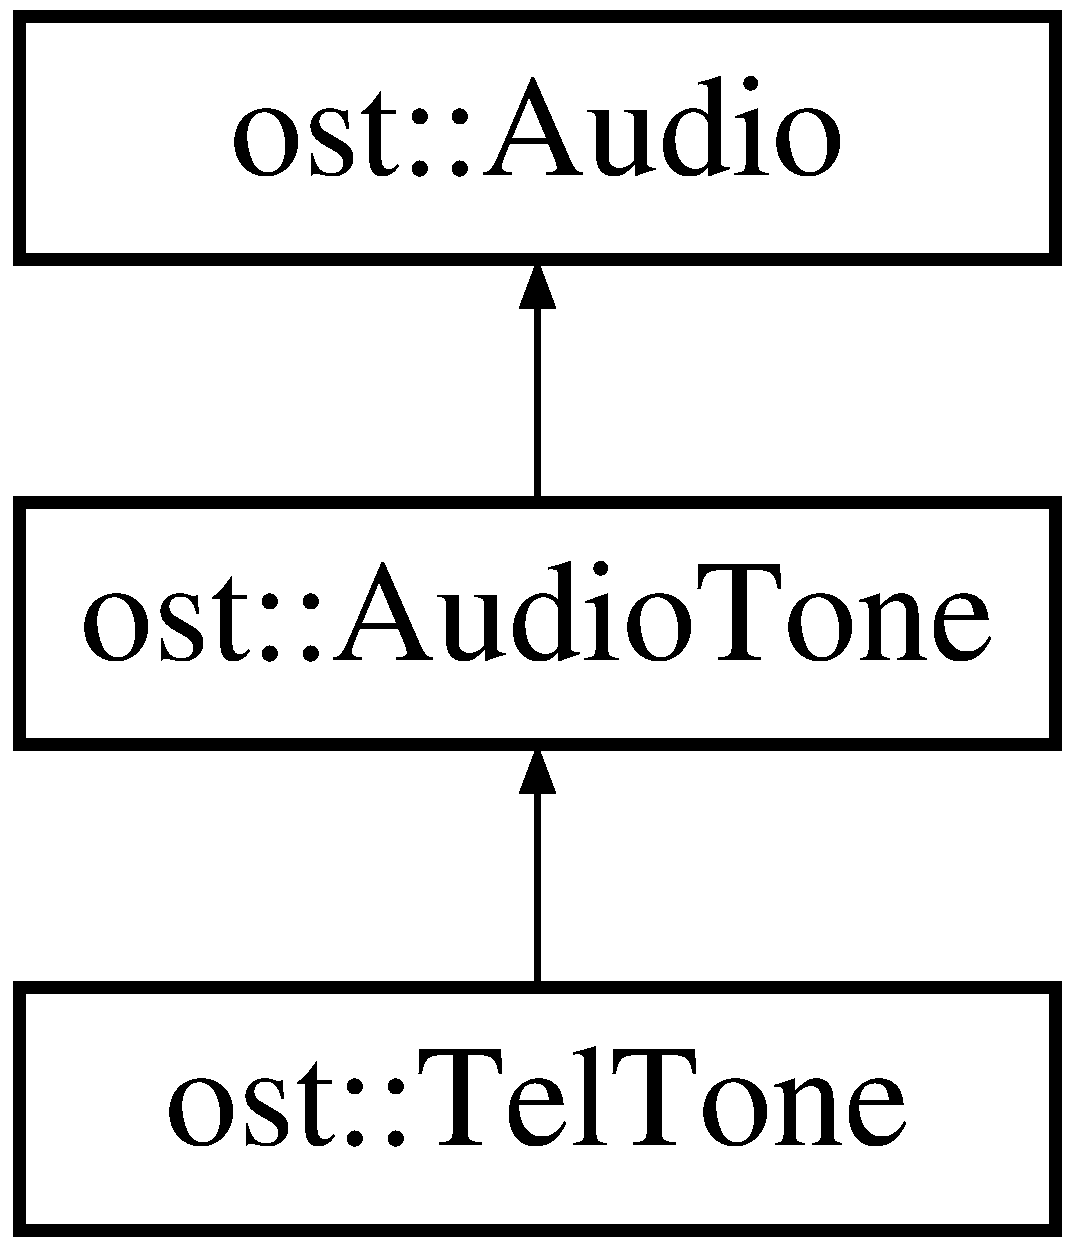
\includegraphics[height=3cm]{classost_1_1_tel_tone}
\end{center}
\end{figure}
\subsection*{Classes}
\begin{DoxyCompactItemize}
\item 
struct {\bf \_\-tonedef}
\item 
struct {\bf \_\-tonekey}
\end{DoxyCompactItemize}
\subsection*{Public Types}
\begin{DoxyCompactItemize}
\item 
typedef struct {\bf ost::TelTone::\_\-tonedef} {\bf tonedef\_\-t}
\item 
typedef struct {\bf ost::TelTone::\_\-tonekey} {\bf tonekey\_\-t}
\end{DoxyCompactItemize}
\subsection*{Public Member Functions}
\begin{DoxyCompactItemize}
\item 
{\bf TelTone} ({\bf tonekey\_\-t} $\ast$key, {\bf Level} {\bf level}, {\bf timeout\_\-t} {\bf frame}=20)
\begin{DoxyCompactList}\small\item\em Create a tone sequencing object for a specific telephony tone key id. \item\end{DoxyCompactList}\item 
{\bf $\sim$TelTone} ()
\item 
{\bf Linear} {\bf getFrame} (void)
\begin{DoxyCompactList}\small\item\em Generate and retrieve one frame of linear audio data for the telephony tone sequence being created. \item\end{DoxyCompactList}\item 
bool {\bf isComplete} (void)
\begin{DoxyCompactList}\small\item\em Check if all audio frames for this tone has been created. \item\end{DoxyCompactList}\end{DoxyCompactItemize}
\subsection*{Static Public Member Functions}
\begin{DoxyCompactItemize}
\item 
static bool {\bf load} (const char $\ast$pathname, const char $\ast$locale=NULL)
\begin{DoxyCompactList}\small\item\em Load a teltones database file into memory. \item\end{DoxyCompactList}\item 
static {\bf tonekey\_\-t} $\ast$ {\bf find} (const char $\ast${\bf tone}, const char $\ast$locale=NULL)
\begin{DoxyCompactList}\small\item\em find an entry in the teltones database. \item\end{DoxyCompactList}\end{DoxyCompactItemize}
\subsection*{Protected Attributes}
\begin{DoxyCompactItemize}
\item 
{\bf tonekey\_\-t} $\ast$ {\bf tone}
\item 
{\bf tonedef\_\-t} $\ast$ {\bf def}
\item 
unsigned {\bf remaining}
\item 
unsigned {\bf silent}
\item 
unsigned {\bf count}
\item 
{\bf timeout\_\-t} {\bf framing}
\item 
{\bf Level} {\bf level}
\item 
bool {\bf complete}
\end{DoxyCompactItemize}


\subsection{Detailed Description}
An object that is used to sequence and extract telephony tones based on a telephony tone descriptor retrieved from the parsed international telephony tone database. \begin{DoxyAuthor}{Author}
David Sugar $<${\tt dyfet@ostel.com}$>$ telephony tone sequencing object. 
\end{DoxyAuthor}


\subsection{Member Typedef Documentation}
\index{ost::TelTone@{ost::TelTone}!tonedef\_\-t@{tonedef\_\-t}}
\index{tonedef\_\-t@{tonedef\_\-t}!ost::TelTone@{ost::TelTone}}
\subsubsection[{tonedef\_\-t}]{\setlength{\rightskip}{0pt plus 5cm}typedef struct {\bf ost::TelTone::\_\-tonedef}  {\bf ost::TelTone::tonedef\_\-t}}\label{classost_1_1_tel_tone_a68db377979005fe801d50f07f0e03be5}
\index{ost::TelTone@{ost::TelTone}!tonekey\_\-t@{tonekey\_\-t}}
\index{tonekey\_\-t@{tonekey\_\-t}!ost::TelTone@{ost::TelTone}}
\subsubsection[{tonekey\_\-t}]{\setlength{\rightskip}{0pt plus 5cm}typedef struct {\bf ost::TelTone::\_\-tonekey}  {\bf ost::TelTone::tonekey\_\-t}}\label{classost_1_1_tel_tone_af77f6282aa08dc65e4db2834bfeac473}


\subsection{Constructor \& Destructor Documentation}
\index{ost::TelTone@{ost::TelTone}!TelTone@{TelTone}}
\index{TelTone@{TelTone}!ost::TelTone@{ost::TelTone}}
\subsubsection[{TelTone}]{\setlength{\rightskip}{0pt plus 5cm}ost::TelTone::TelTone ({\bf tonekey\_\-t} $\ast$ {\em key}, \/  {\bf Level} {\em level}, \/  {\bf timeout\_\-t} {\em frame} = {\ttfamily 20})}\label{classost_1_1_tel_tone_a9a8adaa958dfa572f6d6f5c8e1d3b072}


Create a tone sequencing object for a specific telephony tone key id. 
\begin{DoxyParams}{Parameters}
\item[{\em key}]for telephony tone. \item[{\em level}]for generated tones. \item[{\em frame}]timing to use in processing. \end{DoxyParams}
\index{ost::TelTone@{ost::TelTone}!$\sim$TelTone@{$\sim$TelTone}}
\index{$\sim$TelTone@{$\sim$TelTone}!ost::TelTone@{ost::TelTone}}
\subsubsection[{$\sim$TelTone}]{\setlength{\rightskip}{0pt plus 5cm}ost::TelTone::$\sim$TelTone ()}\label{classost_1_1_tel_tone_a1ebc07f54bafd5b7d901b8bdbf201bab}


\subsection{Member Function Documentation}
\index{ost::TelTone@{ost::TelTone}!find@{find}}
\index{find@{find}!ost::TelTone@{ost::TelTone}}
\subsubsection[{find}]{\setlength{\rightskip}{0pt plus 5cm}static {\bf tonekey\_\-t}$\ast$ ost::TelTone::find (const char $\ast$ {\em tone}, \/  const char $\ast$ {\em locale} = {\ttfamily NULL})\hspace{0.3cm}{\ttfamily  [static]}}\label{classost_1_1_tel_tone_a20f6472d7864f980c2d6040ef5a38cc1}


find an entry in the teltones database. \begin{DoxyReturn}{Returns}
key of tone list if found, else NULL 
\end{DoxyReturn}

\begin{DoxyParams}{Parameters}
\item[{\em tone}]name \item[{\em locale}]to optionally search under \end{DoxyParams}
\index{ost::TelTone@{ost::TelTone}!getFrame@{getFrame}}
\index{getFrame@{getFrame}!ost::TelTone@{ost::TelTone}}
\subsubsection[{getFrame}]{\setlength{\rightskip}{0pt plus 5cm}{\bf Linear} ost::TelTone::getFrame (void)\hspace{0.3cm}{\ttfamily  [virtual]}}\label{classost_1_1_tel_tone_a9fb42cc64137389c3033b58505a5a6d9}


Generate and retrieve one frame of linear audio data for the telephony tone sequence being created. \begin{DoxyReturn}{Returns}
pointer to samples generated. 
\end{DoxyReturn}


Reimplemented from {\bf ost::AudioTone} \doxyref{}{p.}{classost_1_1_audio_tone_a943d31930ce0f1318f42d6dc825200cb}.\index{ost::TelTone@{ost::TelTone}!isComplete@{isComplete}}
\index{isComplete@{isComplete}!ost::TelTone@{ost::TelTone}}
\subsubsection[{isComplete}]{\setlength{\rightskip}{0pt plus 5cm}bool ost::TelTone::isComplete (void)\hspace{0.3cm}{\ttfamily  [virtual]}}\label{classost_1_1_tel_tone_ac9a38161400d6a843d4b38a819ae48e9}


Check if all audio frames for this tone has been created. Some telephony tones, such as dialtone, may be infinite...

\begin{DoxyReturn}{Returns}
true if audio is complete. 
\end{DoxyReturn}


Reimplemented from {\bf ost::AudioTone} \doxyref{}{p.}{classost_1_1_audio_tone_afd2f4d74c504ff9f1638ac0097f7df8d}.\index{ost::TelTone@{ost::TelTone}!load@{load}}
\index{load@{load}!ost::TelTone@{ost::TelTone}}
\subsubsection[{load}]{\setlength{\rightskip}{0pt plus 5cm}static bool ost::TelTone::load (const char $\ast$ {\em pathname}, \/  const char $\ast$ {\em locale} = {\ttfamily NULL})\hspace{0.3cm}{\ttfamily  [static]}}\label{classost_1_1_tel_tone_accdcf48f72d04bc79dc6ee2bfad38b35}


Load a teltones database file into memory. \begin{DoxyReturn}{Returns}
true if successful 
\end{DoxyReturn}

\begin{DoxyParams}{Parameters}
\item[{\em pathname}]of file to load. \item[{\em locale}]to optionally load. \end{DoxyParams}


\subsection{Member Data Documentation}
\index{ost::TelTone@{ost::TelTone}!complete@{complete}}
\index{complete@{complete}!ost::TelTone@{ost::TelTone}}
\subsubsection[{complete}]{\setlength{\rightskip}{0pt plus 5cm}bool {\bf ost::TelTone::complete}\hspace{0.3cm}{\ttfamily  [protected]}}\label{classost_1_1_tel_tone_ab7bf2c032d956281a1ff8dd92eae2acd}
\index{ost::TelTone@{ost::TelTone}!count@{count}}
\index{count@{count}!ost::TelTone@{ost::TelTone}}
\subsubsection[{count}]{\setlength{\rightskip}{0pt plus 5cm}unsigned {\bf ost::TelTone::count}\hspace{0.3cm}{\ttfamily  [protected]}}\label{classost_1_1_tel_tone_ad83573418d7d66ee12ab7742a3427856}
\index{ost::TelTone@{ost::TelTone}!def@{def}}
\index{def@{def}!ost::TelTone@{ost::TelTone}}
\subsubsection[{def}]{\setlength{\rightskip}{0pt plus 5cm}{\bf tonedef\_\-t}$\ast$ {\bf ost::TelTone::def}\hspace{0.3cm}{\ttfamily  [protected]}}\label{classost_1_1_tel_tone_aa83d1aff24fd6bc422275f7f3e638b73}
\index{ost::TelTone@{ost::TelTone}!framing@{framing}}
\index{framing@{framing}!ost::TelTone@{ost::TelTone}}
\subsubsection[{framing}]{\setlength{\rightskip}{0pt plus 5cm}{\bf timeout\_\-t} {\bf ost::TelTone::framing}\hspace{0.3cm}{\ttfamily  [protected]}}\label{classost_1_1_tel_tone_a8b133fbb4fbffc680fccd894405acca0}
\index{ost::TelTone@{ost::TelTone}!level@{level}}
\index{level@{level}!ost::TelTone@{ost::TelTone}}
\subsubsection[{level}]{\setlength{\rightskip}{0pt plus 5cm}{\bf Level} {\bf ost::TelTone::level}\hspace{0.3cm}{\ttfamily  [protected]}}\label{classost_1_1_tel_tone_ac64942aa5d5993948cb89115f2a0e203}
\index{ost::TelTone@{ost::TelTone}!remaining@{remaining}}
\index{remaining@{remaining}!ost::TelTone@{ost::TelTone}}
\subsubsection[{remaining}]{\setlength{\rightskip}{0pt plus 5cm}unsigned {\bf ost::TelTone::remaining}\hspace{0.3cm}{\ttfamily  [protected]}}\label{classost_1_1_tel_tone_a063fcabcb8f53fda15619e590e3f5376}
\index{ost::TelTone@{ost::TelTone}!silent@{silent}}
\index{silent@{silent}!ost::TelTone@{ost::TelTone}}
\subsubsection[{silent}]{\setlength{\rightskip}{0pt plus 5cm}unsigned {\bf ost::TelTone::silent}\hspace{0.3cm}{\ttfamily  [protected]}}\label{classost_1_1_tel_tone_a8992b8689dfc06bbeefce252c018aa7d}
\index{ost::TelTone@{ost::TelTone}!tone@{tone}}
\index{tone@{tone}!ost::TelTone@{ost::TelTone}}
\subsubsection[{tone}]{\setlength{\rightskip}{0pt plus 5cm}{\bf tonekey\_\-t}$\ast$ {\bf ost::TelTone::tone}\hspace{0.3cm}{\ttfamily  [protected]}}\label{classost_1_1_tel_tone_a91d5a785d8f665505d03eac002f246df}


The documentation for this class was generated from the following file:\begin{DoxyCompactItemize}
\item 
{\bf audio2.h}\end{DoxyCompactItemize}

\section{ost::Audio::tone\_\-detection\_\-descriptor\_\-t Struct Reference}
\label{structost_1_1_audio_1_1tone__detection__descriptor__t}\index{ost::Audio::tone\_\-detection\_\-descriptor\_\-t@{ost::Audio::tone\_\-detection\_\-descriptor\_\-t}}


{\ttfamily \#include $<$audio2.h$>$}\subsection*{Public Attributes}
\begin{DoxyCompactItemize}
\item 
float {\bf fac}
\end{DoxyCompactItemize}


\subsection{Member Data Documentation}
\index{ost::Audio::tone\_\-detection\_\-descriptor\_\-t@{ost::Audio::tone\_\-detection\_\-descriptor\_\-t}!fac@{fac}}
\index{fac@{fac}!ost::Audio::tone_detection_descriptor_t@{ost::Audio::tone\_\-detection\_\-descriptor\_\-t}}
\subsubsection[{fac}]{\setlength{\rightskip}{0pt plus 5cm}float {\bf ost::Audio::tone\_\-detection\_\-descriptor\_\-t::fac}}\label{structost_1_1_audio_1_1tone__detection__descriptor__t_a3624c9fe09774dc046df3f268325735e}


The documentation for this struct was generated from the following file:\begin{DoxyCompactItemize}
\item 
{\bf audio2.h}\end{DoxyCompactItemize}

\chapter{File Documentation}
\section{audio2.h File Reference}
\label{audio2_8h}\index{audio2.h@{audio2.h}}


Framework for portable audio processing and file handling classes.  
{\ttfamily \#include $<$cstddef$>$}\par
{\ttfamily \#include $<$cstdlib$>$}\par
{\ttfamily \#include $<$sys/types.h$>$}\par
{\ttfamily \#include $<$netinet/in.h$>$}\par
{\ttfamily \#include $<$ctime$>$}\par
\subsection*{Classes}
\begin{DoxyCompactItemize}
\item 
class {\bf ost::Audio}
\begin{DoxyCompactList}\small\item\em Generic audio class to hold master data types and various useful class encapsulated friend functions as per GNU Common C++ 2 coding standard. \item\end{DoxyCompactList}\item 
struct {\bf ost::Audio::goertzel\_\-state\_\-t}
\item 
struct {\bf ost::Audio::dtmf\_\-detect\_\-state\_\-t}
\item 
struct {\bf ost::Audio::tone\_\-detection\_\-descriptor\_\-t}
\item 
struct {\bf ost::Audio::mpeg\_\-audio}
\item 
struct {\bf ost::Audio::mpeg\_\-tagv1}
\item 
class {\bf ost::Audio::Info}
\begin{DoxyCompactList}\small\item\em \doxyref{Audio}{p.}{classost_1_1_audio} source description. \item\end{DoxyCompactList}\item 
class {\bf ost::AudioResample}
\begin{DoxyCompactList}\small\item\em The \doxyref{AudioResample}{p.}{classost_1_1_audio_resample} class is used to manage linear intropolation buffering for rate conversions. \item\end{DoxyCompactList}\item 
class {\bf ost::AudioTone}
\begin{DoxyCompactList}\small\item\em The \doxyref{AudioTone}{p.}{classost_1_1_audio_tone} class is used to create a frame of audio encoded single or dualtones. \item\end{DoxyCompactList}\item 
class {\bf ost::AudioBase}
\begin{DoxyCompactList}\small\item\em \doxyref{AudioBase}{p.}{classost_1_1_audio_base} base class for many other audio classes which stream data. \item\end{DoxyCompactList}\item 
class {\bf ost::AudioBuffer}
\begin{DoxyCompactList}\small\item\em The \doxyref{AudioBuffer}{p.}{classost_1_1_audio_buffer} class is for mixing one-\/to-\/one soft joins. \item\end{DoxyCompactList}\item 
class {\bf ost::AudioFile}
\begin{DoxyCompactList}\small\item\em A class used to manipulate audio data. \item\end{DoxyCompactList}\item 
class {\bf ost::AudioStream}
\begin{DoxyCompactList}\small\item\em \doxyref{AudioStream}{p.}{classost_1_1_audio_stream} accesses \doxyref{AudioFile}{p.}{classost_1_1_audio_file} base class content as fixed frames of streaming linear samples. \item\end{DoxyCompactList}\item 
class {\bf ost::AudioCodec}
\begin{DoxyCompactList}\small\item\em The codec class is a virtual used for transcoding audio samples between linear frames (or other known format) and an encoded \char`\"{}sample\char`\"{} buffer. \item\end{DoxyCompactList}\item 
class {\bf ost::AudioDevice}
\item 
class {\bf ost::TelTone}
\begin{DoxyCompactList}\small\item\em An object that is used to sequence and extract telephony tones based on a telephony tone descriptor retrieved from the parsed international telephony tone database. \item\end{DoxyCompactList}\item 
struct {\bf ost::TelTone::\_\-tonedef}
\item 
struct {\bf ost::TelTone::\_\-tonekey}
\item 
class {\bf ost::DTMFTones}
\begin{DoxyCompactList}\small\item\em \doxyref{DTMFTones}{p.}{classost_1_1_d_t_m_f_tones} is used to generate a series of dtmf audio data from a \char`\"{}telephone\char`\"{} number passed as an ASCII string. \item\end{DoxyCompactList}\item 
class {\bf ost::MFTones}
\begin{DoxyCompactList}\small\item\em \doxyref{MFTones}{p.}{classost_1_1_m_f_tones} is used to generate a series of mf audio data from a \char`\"{}telephone\char`\"{} number passed as an ASCII string. \item\end{DoxyCompactList}\item 
class {\bf ost::DTMFDetect}
\begin{DoxyCompactList}\small\item\em \doxyref{DTMFDetect}{p.}{classost_1_1_d_t_m_f_detect} is used for detecting DTMF tones in a stream of audio. \item\end{DoxyCompactList}\end{DoxyCompactItemize}
\subsection*{Namespaces}
\begin{DoxyCompactItemize}
\item 
namespace {\bf ost}
\end{DoxyCompactItemize}
\subsection*{Defines}
\begin{DoxyCompactItemize}
\item 
\#define {\bf CCXX\_\-PACKED}
\item 
\#define {\bf AUDIO\_\-SIGNED\_\-LINEAR\_\-RAW}~1
\item 
\#define {\bf AUDIO\_\-LINEAR\_\-CONVERSION}~1
\item 
\#define {\bf AUDIO\_\-CODEC\_\-MODULES}~1
\item 
\#define {\bf AUDIO\_\-LINEAR\_\-FRAMING}~1
\item 
\#define {\bf AUDIO\_\-NATIVE\_\-METHODS}~1
\item 
\#define {\bf AUDIO\_\-RATE\_\-RESAMPLER}~1
\end{DoxyCompactItemize}
\subsection*{Variables}
\begin{DoxyCompactItemize}
\item 
class \_\-\_\-EXPORT {\bf ost::AudioCodec}
\item 
class \_\-\_\-EXPORT {\bf ost::AudioDevice}
\end{DoxyCompactItemize}


\subsection{Detailed Description}
Framework for portable audio processing and file handling classes. 

\subsection{Define Documentation}
\index{audio2.h@{audio2.h}!AUDIO\_\-CODEC\_\-MODULES@{AUDIO\_\-CODEC\_\-MODULES}}
\index{AUDIO\_\-CODEC\_\-MODULES@{AUDIO\_\-CODEC\_\-MODULES}!audio2.h@{audio2.h}}
\subsubsection[{AUDIO\_\-CODEC\_\-MODULES}]{\setlength{\rightskip}{0pt plus 5cm}\#define AUDIO\_\-CODEC\_\-MODULES~1}\label{audio2_8h_a028536012084a42b4510c90eb28be738}
\index{audio2.h@{audio2.h}!AUDIO\_\-LINEAR\_\-CONVERSION@{AUDIO\_\-LINEAR\_\-CONVERSION}}
\index{AUDIO\_\-LINEAR\_\-CONVERSION@{AUDIO\_\-LINEAR\_\-CONVERSION}!audio2.h@{audio2.h}}
\subsubsection[{AUDIO\_\-LINEAR\_\-CONVERSION}]{\setlength{\rightskip}{0pt plus 5cm}\#define AUDIO\_\-LINEAR\_\-CONVERSION~1}\label{audio2_8h_a84606f4a23e81410b0e32e486822f846}
\index{audio2.h@{audio2.h}!AUDIO\_\-LINEAR\_\-FRAMING@{AUDIO\_\-LINEAR\_\-FRAMING}}
\index{AUDIO\_\-LINEAR\_\-FRAMING@{AUDIO\_\-LINEAR\_\-FRAMING}!audio2.h@{audio2.h}}
\subsubsection[{AUDIO\_\-LINEAR\_\-FRAMING}]{\setlength{\rightskip}{0pt plus 5cm}\#define AUDIO\_\-LINEAR\_\-FRAMING~1}\label{audio2_8h_a24e608854dc0dd9bcbc44a4a4dcdf676}
\index{audio2.h@{audio2.h}!AUDIO\_\-NATIVE\_\-METHODS@{AUDIO\_\-NATIVE\_\-METHODS}}
\index{AUDIO\_\-NATIVE\_\-METHODS@{AUDIO\_\-NATIVE\_\-METHODS}!audio2.h@{audio2.h}}
\subsubsection[{AUDIO\_\-NATIVE\_\-METHODS}]{\setlength{\rightskip}{0pt plus 5cm}\#define AUDIO\_\-NATIVE\_\-METHODS~1}\label{audio2_8h_ac9fbed88006882c27fe7d228291c8c7c}
\index{audio2.h@{audio2.h}!AUDIO\_\-RATE\_\-RESAMPLER@{AUDIO\_\-RATE\_\-RESAMPLER}}
\index{AUDIO\_\-RATE\_\-RESAMPLER@{AUDIO\_\-RATE\_\-RESAMPLER}!audio2.h@{audio2.h}}
\subsubsection[{AUDIO\_\-RATE\_\-RESAMPLER}]{\setlength{\rightskip}{0pt plus 5cm}\#define AUDIO\_\-RATE\_\-RESAMPLER~1}\label{audio2_8h_abe8f760f29265ae92d19dc703e031f67}
\index{audio2.h@{audio2.h}!AUDIO\_\-SIGNED\_\-LINEAR\_\-RAW@{AUDIO\_\-SIGNED\_\-LINEAR\_\-RAW}}
\index{AUDIO\_\-SIGNED\_\-LINEAR\_\-RAW@{AUDIO\_\-SIGNED\_\-LINEAR\_\-RAW}!audio2.h@{audio2.h}}
\subsubsection[{AUDIO\_\-SIGNED\_\-LINEAR\_\-RAW}]{\setlength{\rightskip}{0pt plus 5cm}\#define AUDIO\_\-SIGNED\_\-LINEAR\_\-RAW~1}\label{audio2_8h_a1cba749dac4075b565ef27f32000af1c}
\index{audio2.h@{audio2.h}!CCXX\_\-PACKED@{CCXX\_\-PACKED}}
\index{CCXX\_\-PACKED@{CCXX\_\-PACKED}!audio2.h@{audio2.h}}
\subsubsection[{CCXX\_\-PACKED}]{\setlength{\rightskip}{0pt plus 5cm}\#define CCXX\_\-PACKED}\label{audio2_8h_a2d5d6a19f6c727b9e318292caa8b7f4d}

\printindex
\end{document}
